%Version 3.1 December 2024
% See section 11 of the User Manual for version history
%
%%%%%%%%%%%%%%%%%%%%%%%%%%%%%%%%%%%%%%%%%%%%%%%%%%%%%%%%%%%%%%%%%%%%%%
%%                                                                 %%
%% Please do not use \input{...} to include other tex files.       %%
%% Submit your LaTeX manuscript as one .tex document.              %%
%%                                                                 %%
%% All additional figures and files should be attached             %%
%% separately and not embedded in the \TeX\ document itself.       %%
%%                                                                 %%
%%%%%%%%%%%%%%%%%%%%%%%%%%%%%%%%%%%%%%%%%%%%%%%%%%%%%%%%%%%%%%%%%%%%%

%%\documentclass[referee,sn-basic]{sn-jnl}% referee option is meant for double line spacing

%%=======================================================%%
%% to print line numbers in the margin use lineno option %%
%%=======================================================%%

%%\documentclass[lineno,pdflatex,sn-basic]{sn-jnl}% Basic Springer Nature Reference Style/Chemistry Reference Style

%%=========================================================================================%%
%% the documentclass is set to pdflatex as default. You can delete it if not appropriate.  %%
%%=========================================================================================%%

%%\documentclass[sn-basic]{sn-jnl}% Basic Springer Nature Reference Style/Chemistry Reference Style

%%Note: the following reference styles support Namedate and Numbered referencing. By default the style follows the most common style. To switch between the options you can add or remove �Numbered� in the optional parenthesis. 
%%The option is available for: sn-basic.bst, sn-chicago.bst%  
 
%%\documentclass[pdflatex,sn-nature]{sn-jnl}% Style for submissions to Nature Portfolio journals
%%\documentclass[pdflatex,sn-basic]{sn-jnl}% Basic Springer Nature Reference Style/Chemistry Reference Style
\documentclass[pdflatex,sn-mathphys-num]{sn-jnl}% Math and Physical Sciences Numbered Reference Style
%%\documentclass[pdflatex,sn-mathphys-ay]{sn-jnl}% Math and Physical Sciences Author Year Reference Style
%%\documentclass[pdflatex,sn-aps]{sn-jnl}% American Physical Society (APS) Reference Style
%%\documentclass[pdflatex,sn-vancouver-num]{sn-jnl}% Vancouver Numbered Reference Style
%%\documentclass[pdflatex,sn-vancouver-ay]{sn-jnl}% Vancouver Author Year Reference Style
%%\documentclass[pdflatex,sn-apa]{sn-jnl}% APA Reference Style
%%\documentclass[pdflatex,sn-chicago]{sn-jnl}% Chicago-based Humanities Reference Style

%%%% Standard Packages
%%<additional latex packages if required can be included here>

\usepackage{graphicx}%
\usepackage{multirow}%
% \usepackage{amsmath,amssymb,amsfonts}%
\usepackage{amssymb,amsfonts}%
\usepackage{amsthm}%
\usepackage{mathrsfs}%
\usepackage[title]{appendix}%
\usepackage{xcolor}%
\usepackage{textcomp}%
\usepackage{manyfoot}%
\usepackage{booktabs}%
\usepackage{algorithm}%
\usepackage{algorithmicx}%
\usepackage{algpseudocode}%
\usepackage{listings}%

%%%% EXTRA %%%%%
\usepackage{mathtools} % also loads\usepackage{amsmath}
\usepackage{amssymb}	% Extra maths symbols
\usepackage{siunitx}
\usepackage{float}
\usepackage{physics}
%\usepackage[version=4]{mhchem}
\usepackage{bm} %new
\usepackage{booktabs}
\usepackage{xcolor}
\usepackage{derivative} % for \pdv

% Tikz
\usepackage{tikz}
\usetikzlibrary{positioning}
\usepackage{listofitems} % for \readlist to create arrays
\usetikzlibrary{arrows.meta} % for arrow size
\usepackage{tikz-3dplot} % for 3D plotting and Euler angle handling
\usepackage{subcaption} % provides the subfigure / subtable environments
% \usepackage{natbib,twoopt}

% Macros
\newcommand{\degr}{\ensuremath{^\circ}}
\newcommand{\arcmin}{\ensuremath{^{\prime}}}
\newcommand{\sun}{\odot}
\newcommand{\earth}{\oplus}
\newcommand{\micron}{\ensuremath{\mu\mathrm{m}}}

% Journal name macros 
\def\aap{A\&A}
\def\aaps{A\&AS}
\def\aapr{A\&ARv}
\def\actaa{Acta Astron.}
\def\aj{AJ}
\def\ao{Appl. Opt.}
\def\apj{ApJ}
\def\apjl{ApJL}
\def\apjs{ApJS}
\def\araa{ARA\&A}
\def\baas{BAAS}
\def\icarus{Icarus}
\def\jgr{J. Geophys. Res.}
\def\mnras{MNRAS}
\def\nat{Nature}
\def\nphysa{Nucl. Phys. A}
\def\planss{Planet. Space Sci.}
\def\pra{Phys. Rev. A}
\def\prb{Phys. Rev. B}
\def\prc{Phys. Rev. C}
\def\prd{Phys. Rev. D}
\def\pre{Phys. Rev. E}
\def\prl{Phys. Rev. Lett.}
\def\pasj{PASJ}
\def\pasp{PASP}
\def\solphys{Sol. Phys.}
\def\ssr{Space Sci. Rev.}
\def\grl{Geophys. Res. Lett.}


%%%%%=============================================================================%%%%
%%%%  Remarks: This template is provided to aid authors with the preparation
%%%%  of original research articles intended for submission to journals published 
%%%%  by Springer Nature. The guidance has been prepared in partnership with 
%%%%  production teams to conform to Springer Nature technical requirements. 
%%%%  Editorial and presentation requirements differ among journal portfolios and 
%%%%  research disciplines. You may find sections in this template are irrelevant 
%%%%  to your work and are empowered to omit any such section if allowed by the 
%%%%  journal you intend to submit to. The submission guidelines and policies 
%%%%  of the journal take precedence. A detailed User Manual is available in the 
%%%%  template package for technical guidance.
%%%%%=============================================================================%%%%

%% as per the requirement new theorem styles can be included as shown below
\theoremstyle{thmstyleone}%
\newtheorem{theorem}{Theorem}%  meant for continuous numbers
%%\newtheorem{theorem}{Theorem}[section]% meant for sectionwise numbers
%% optional argument [theorem] produces theorem numbering sequence instead of independent numbers for Proposition
\newtheorem{proposition}[theorem]{Proposition}% 
%%\newtheorem{proposition}{Proposition}% to get separate numbers for theorem and proposition etc.

\theoremstyle{thmstyletwo}%
\newtheorem{example}{Example}%
\newtheorem{remark}{Remark}%

\theoremstyle{thmstylethree}%
\newtheorem{definition}{Definition}%

% Macros
\def\ce#1{\ensuremath{#1}}
\let\unit\si

\DeclareMathOperator{\atantwo}{atan2}


\renewcommand{\vec}[1]{\boldsymbol{#1}}

\raggedbottom
%%\unnumbered% uncomment this for unnumbered level heads

\begin{document}

\title[A Geodesic Formulation for the Rotational Dynamics]{A Geodesic Formulation for the Rotational Dynamics of Tidally Deformable Bodies: Application to Laser Altimetry}

%%=============================================================%%
%% GivenName	-> \fnm{Joergen W.}
%% Particle	-> \spfx{van der} -> surname prefix
%% FamilyName	-> \sur{Ploeg}
%% Suffix	-> \sfx{IV}
%% \author*[1,2]{\fnm{Joergen W.} \spfx{van der} \sur{Ploeg} 
%%  \sfx{IV}}\email{iauthor@gmail.com}
%%=============================================================%%

\author[1,2]{\fnm{Stefano} \sur{Casotto}}

\author*[1]{\fnm{Giulio} \sur{Macrì}}\email{giulio.macri@phd.unipd.it}

\affil*[1]{\orgdiv{Dipartimento di Fisica e Astronomia “Galileo Galilei”}, 
\orgname{Università di Padova}, 
\orgaddress{\street{Vicolo dell'Osservatorio 3}, \city{Padova}, \postcode{35122}, \country{Italy}}}

\affil[2]{\orgdiv{Centro di Ateneo di Studi e Attività Spaziali “Giuseppe Colombo” (CISAS)}, 
\orgname{Università di Padova}, 
\orgaddress{\street{Via Venezia 15}, \city{Padova}, \postcode{35131}, \country{Italy}}}

% \affil[3]{\orgdiv{Institute of Space Research}, 
% \orgname{German Aerospace Center (DLR)}, 
% \orgaddress{\street{Rutherfordstraße 2}, \city{Berlin}, \postcode{12489}, \country{Germany}}}

%% TEMPLATE %%%
% \author*[1,2]{\fnm{First} \sur{Author}}\email{iauthor@gmail.com}

% \author[2,3]{\fnm{Second} \sur{Author}}\email{iiauthor@gmail.com}
% \equalcont{These authors contributed equally to this work.}

% \author[1,2]{\fnm{Third} \sur{Author}}\email{iiiauthor@gmail.com}
% \equalcont{These authors contributed equally to this work.}

% \affil*[1]{\orgdiv{Department}, \orgname{Organization}, \orgaddress{\street{Street}, \city{City}, \postcode{100190}, \state{State}, \country{Country}}}

% \affil[2]{\orgdiv{Department}, \orgname{Organization}, \orgaddress{\street{Street}, \city{City}, \postcode{10587}, \state{State}, \country{Country}}}

% \affil[3]{\orgdiv{Department}, \orgname{Organization}, \orgaddress{\street{Street}, \city{City}, \postcode{610101}, \state{State}, \country{Country}}}

%%==================================%%
%% Sample for unstructured abstract %%
%%==================================%%

\abstract{
The precise determination of the rotational state of celestial bodies is a fundamental requirement for constraining their internal structure, particularly for the icy moons of the outer solar system targeted by upcoming missions like Juice and Europa Clipper. While the rotational dynamics of rigid bodies are well-described by the classic Euler-Liouville equations, modeling non-rigid effects—such as tidal deformations and coupling with subsurface fluid layers—often requires complex ad-hoc modifications to the inertia tensor and torque vectors. In this work, we present a rigorous alternative formulation based on Lagrangian mechanics on a Riemannian manifold. By treating the Euler angles as generalized coordinates, we demonstrate that the rotational motion describes a geodesic in the configuration space. Furthermore, we show that when tidal and centrifugal deformations are explicitly modeled, the metric tensor becomes dependent on both the generalized coordinates and their velocities, effectively transitioning the dynamical framework from Riemannian to Finsler geometry. This geometric approach naturally encapsulates the coupling between orbital position, rotation, and deformation without the need for time-dependent forcing terms in the angular momentum equation. We derive the full set of equations of motion and the associated variational equations required for precise state estimation. Finally, we validate the practical utility of this framework through a covariance analysis of a Ganymede-like body. Simulating laser altimetry data, we demonstrate that the principal moments of inertia and libration amplitudes are observable and can be decorrelated with sufficient tracking duration, providing a robust mathematical foundation for future geophysical investigations.
}

% \abstract{The abstract serves both as a general introduction to the topic and as a brief, non-technical summary of the main results and their implications. Authors are advised to check the author instructions for the journal they are submitting to for word limits and if structural elements like subheadings, citations, or equations are permitted.}

%%================================%%
%% Sample for structured abstract %%
%%================================%%

% \abstract{\textbf{Purpose:} The abstract serves both as a general introduction to the topic and as a brief, non-technical summary of the main results and their implications. The abstract must not include subheadings (unless expressly permitted in the journal's Instructions to Authors), equations or citations. As a guide the abstract should not exceed 200 words. Most journals do not set a hard limit however authors are advised to check the author instructions for the journal they are submitting to.
% 
% \textbf{Methods:} The abstract serves both as a general introduction to the topic and as a brief, non-technical summary of the main results and their implications. The abstract must not include subheadings (unless expressly permitted in the journal's Instructions to Authors), equations or citations. As a guide the abstract should not exceed 200 words. Most journals do not set a hard limit however authors are advised to check the author instructions for the journal they are submitting to.
% 
% \textbf{Results:} The abstract serves both as a general introduction to the topic and as a brief, non-technical summary of the main results and their implications. The abstract must not include subheadings (unless expressly permitted in the journal's Instructions to Authors), equations or citations. As a guide the abstract should not exceed 200 words. Most journals do not set a hard limit however authors are advised to check the author instructions for the journal they are submitting to.
% 
% \textbf{Conclusion:} The abstract serves both as a general introduction to the topic and as a brief, non-technical summary of the main results and their implications. The abstract must not include subheadings (unless expressly permitted in the journal's Instructions to Authors), equations or citations. As a guide the abstract should not exceed 200 words. Most journals do not set a hard limit however authors are advised to check the author instructions for the journal they are submitting to.}

% \keywords{keyword1, Keyword2, Keyword3, Keyword4}
\keywords{Rotational dynamics, Ganymede, Laser altimetry, Covariance analysis}

%%\pacs[JEL Classification]{D8, H51}

%%\pacs[MSC Classification]{35A01, 65L10, 65L12, 65L20, 65L70}

\maketitle


% The rotational dynamics of celestial bodies are traditionally modeled using the Euler-Liouville equations for the angular velocities. While effective for rigid bodies, this approach becomes cumbersome when dealing with non-rigid effects such as tidal deformations, internal mass redistribution, or coupling with fluid layers. In these scenarios, the inertia tensor becomes time-dependent and state-dependent, leading to complex additional torque terms in the angular velocity formulation.

% In this work, we propose an alternative formulation based on the Lagrangian mechanics on a Riemannian manifold. By treating the Euler angles as generalized coordinates, the rotational motion describes a geodesic in the configuration space equipped with a specific metric tensor. We show that when tidal deformations are included, the metric tensor becomes dependent on both the coordinates and their velocities, effectively moving the problem into the realm of Finsler geometry.

% This formulation offers distinct advantages: it naturally handles the "breathing" of the metric due to tides without requiring ad-hoc torque corrections, and it facilitates the computation of the state transition matrix required for precise orbit determination and parameter estimation.

% We apply this framework to a covariance analysis of a Ganymede-like body, investigating the observability of the inertia tensor and libration amplitudes using laser altimetry data similar to that expected from the Juice mission.


\section{Introduction}

The exploration of the Galilean satellites has entered a new era with the European Space Agency's Jupiter Icy Moons Explorer (Juice) and NASA's Europa Clipper missions. A primary scientific objective of these missions is to characterize the interior structure of these moons, specifically to confirm the existence and extent of subsurface liquid oceans \citep{2020P&SS..18704902C}. The rotational state of a satellite—specifically its physical librations and obliquity—is intimately coupled to its internal mass distribution and rheology. Consequently, the precise estimation of these rotational parameters is a powerful geodetic tool for probing the deep interior \citep{2010Icar..209..651B, 2011A&A...527A.118R}.

Traditionally, the rotational dynamics of celestial bodies are modeled using the Euler-Liouville equations for the angular velocities. While this approach is robust for rigid bodies, it becomes mathematically cumbersome when dealing with non-rigid effects. For a real planetary body, the inertia tensor is not constant; it varies due to tidal periodicities induced by the central body and the centrifugal deformation caused by the body's own rotation. In the standard Euler formulation, these variations must be treated either as time-dependent modifications to the inertia tensor or as additional fictitious torques on the right-hand side of the equations of motion \citep{2001JGR...10627933W}. This separation can complicate the derivation of the variational equations (the state transition matrix) required for the non-linear least squares estimation of physical parameters.

In this work, we propose an alternative formulation based on Lagrangian mechanics. By treating the Euler angles as generalized coordinates, the rotational motion can be viewed as a geodesic flow on a configuration manifold equipped with a specific metric tensor defined by the mass distribution. This "Geodesic" formulation has been explored for rigid bodies \citep{Broucke1990doi:10.2514/3.20591}, but its extension to deformable bodies remains underutilized in planetary geodesy.

We demonstrate that when tidal and centrifugal deformations are included, the metric tensor of the configuration space becomes dependent not only on the coordinates (orientation) but also on the velocities (spin rate). In the language of differential geometry, this moves the problem from a Riemannian manifold to a Finsler manifold \citep{2006math......2383M}. This geometric perspective offers distinct advantages: it naturally handles the "breathing" of the metric due to tides without ad-hoc corrections, and it provides a unified framework for deriving the partial derivatives needed for orbit determination.

The paper is organized as follows. In Section~\ref{sec:ref_frame}, we define the reference frames and the rigid body metric. In Section~\ref{sec:rot_eq}, we derive the equations of motion in the geodesic form and explicitly extend the metric to account for tidal and centrifugal distortions, introducing the Finsler formulation. In Section~\ref{sec:ocean_rayleigh}, we incorporate the effects of ocean coupling via a Rayleigh dissipation function. Finally, in Section 5, we apply this framework to a covariance analysis of a Ganymede-like body, investigating the observability of the inertia tensor using simulated laser altimetry data similar to that expected from the GALA instrument on Juice.
	
% 	%Our  aim  is that of improving  the  techniques to determine the rotational state, the moments of inertia and other geophysical parameters of Ganymede  in preparation for the JUpiter Icy Moons Explorer (Juice), with a focus on altimetric measurements that will be available thanks to the GAnymede Laser Altimeter (GALA).
	
% 	Among all the solid bodies in the Solar System, Ganymede has the smallest normalized polar moment of inertia, suggesting that the interior of Ganymede is most likely fully differentiated \citep{1996Natur.384..541A}. 
% 	When a subsurface ocean and/or a fluid core exists, the solid layers (shell, mantle and solid core) and the fluid layers (ocean and fluid core) can perform different rotation variations. However, they are coupled with each other through viscous, electromagnetic, pressure and gravitational torques. The viscous torques due to friction forces on the boundaries of the internal ocean and liquid core depend on the small ocean and liquid core viscosity that acts on timescales much larger  than the libration periods. As a result, viscous torques cannot effectively couple solid to liquid layers at the libration periods and we hereafter neglect viscosity in the liquid layers which do not take part in the libration \citep{2010Icar..209..651B}. 
% 	For similar reasons we neglect the electromagnetic torque, although the electromagnetic field generated in the core of Ganymede could be large. The interaction among  the different layers  is then due to the pressure force of the liquid layers on their boundaries, and the gravitational coupling between layers is different from zero only when the layers are not aligned \citep{2010Icar..209..651B}.
% 	Moreover it has been shown that the long period librations are almost insensitive to the interior structure \citep{2011CeMDA.109...85R}. 
	
	
%\section{State of the Art}
	
% 	%Initially we focus on the estimation of the moments of inertia. For simplicity we begin with a rigid body formulation. However it is important to keep in mind that such a formulation may be inadequate to model the librations of Ganymede. 
% 	%Indeed if the long-speculated subsurface global liquid ocean is present underneath the ice crust, then the libration of the icy shell may be fully decoupled from the interior layers. 
	
% 	%The primary objective of this research is to develop innovative estimation techniques to extrapolate information about the rotational and tidal dynamics in order to constrain the internal structure of celestial bodies, specifically focusing on Ganymede, in preparation for the arrival of the Juice spacecraft in the Jovian system in the next decade.
	
	
	
% 	%Using the data from the MESSENGER mission, \cite{Stark2015} demonstrated the effectiveness of coregistering Digital Terrain Models (DTMs) created using the Mercury Dual Imaging System (MDIS) and the altimetric data from the Mercury Laser Altimeter (MLA)
% 	%%onboard MESSENGER,  
% 	%to determine the physical librations of Mercury,  i.e.,  small oscillations  relative to the 
% 	%synchronous
% 	%%mean 
% 	%rotation, that revealed significant details about Mercury’s internal structure.
% 	%
% 	%\cite{2019Geosc...9..320S} showed that accurate measurements of Ganymede's librations could constrain the thickness of an elastic ice shell,  with an accuracy of 24 to 63 km. In the more optimistic range of this error interval, the physical librations would be a valuable constraint on the outer ice shell in combination with the measurement of the tidal Love number $h_2$.
% 	%
	
	
	
	

	
% 	The librations as detected from the coregistration of altimetric profiles are sensitive only to the motion of the outer shell, 
% 	In a body fixed-frame $\mathcal{I}$, the Euler equations for the angular velocities of the outer shell take the form
% 	\begin{equation} \label{eq:euler_solid_moon_williams}
% 		\frac{d(\mathbf{I}_s \vb*{\omega}_s)}{dt} + \vb*{\omega}_s \times(\mathbf{I}_s \vb*{\omega}_s) = \mathbf{K},
% 	\end{equation}
% 	%
% 	where $\mathbf{I}_s$ is the moment of inertia matrix for the outer shell, $\boldsymbol{\omega}_s$ is the shell vector angular velocity, the product $\mathbf{I}_s \boldsymbol{\omega}_s$ is the shell angular momentum vector, and $\mathbf{K}$ is the torque vector. 
% 	The torque vector can be decomposed in the sum of external gravitational  torques $\mathbf{K}_{e}$, that depend on the whole-body degree-2 gravity field coefficients $C_{2m}, S_{2m}$, and internal torques $\mathbf{K}_i$, due to the interaction of the outer shell with the internal layers.
% 	%
% 	The inertia tensor of the shell  varies in time due to the 
% 	tidal distortion by Jupiter,  the Sun, the other Galileian satellites  and spin distortion
% 	\begin{align}
% 		\label{eq:inertia_tidal_spin}
% 		\mathbf{I}_s(t) &= %\mathbf{I}_{s,\mathrm{undistorted}}  + 	\mathbf{I}_{s,\mathrm{tide}}(t)+ \mathbf{I}_{s,\mathrm{spin}}(t)
% 		%\\ &=
% 		\mathbf{\tilde{I}}_{s}  - \displaystyle\sum_i\frac{k_2 m_i R^5}{r_i^5}
% 		\left(  \mathbf{r}_i\mathbf{r}_i- \frac{\mathbb{I}_{3x3}}{3} \right)
% 		\\   &\quad+ \frac{k_2 R^5}{3G}  \left( \vb*{\omega}_s  \vb*{\omega}_s   - \frac{\omega_s^2\mathbb{I}_{3x3}}{3}    	+ \mathrm{diag}(n^2,n^2,-2n^2)   \right),
% 		\notag
% 	\end{align}
% 	%
% 	where $\mathbf{\tilde{I}}_{s} $ is the (constant) undistorted tensor of inertia,
% 	$k_2$ is the Ganymede potential Love number, $R$ the reference radius of Ganymede,  \( \mathbf{r}_i\) is the position vector of the tide raising body $i$ relative to Ganymede, $n$ is the mean motion of Ganymede. The $\mathbf{r}_i i$ and \(\bm{\omega}_s\) terms in equation (\ref{eq:inertia_tidal_spin}) are evaluated at time $t-\tau_s$  to account for the delayed response of the spin and tidal deformation due to dissipation \citep{2001JGR...10627933W}.
% 	%
% 	The Euler equations (\ref{eq:euler_solid_moon_williams}) are expressed  frame $\mathcal{B}$ and are given in the angular velocities variables $\vb*{\omega}_s = (\omega_1,\omega_2,\omega_3)$.
% 	In practice the angular velocities alone are of little use to us, in fact we are more interested in the
% 	In practice we are interested  in the orientation of Ganymede in an inertial frame, described by the Euler angles, i.e., the physical librations. Thus we find it preferable to replace the Euler equations (\ref{eq:euler_solid_moon_williams}) with a set of second order ordinary differential equations (ODEs) for the Euler angles only. The angular velocities are related to the $(3,1,3)$ set of Euler angles $\vb*{\Phi}  = (\phi,\theta,\psi)$ through the following set of first order ODEs
% 	\begin{align}\label{eq:deuler_omega}
% 		\begin{pmatrix}
% 			\dot{\phi} \\
% 			\dot{\theta} \\
% 			\dot{\psi}
% 		\end{pmatrix}
% 		%	= J
% 		%	\begin{pmatrix}
% 			%		\omega_1 \\
% 			%		\omega_2 \\
% 			%		\omega_3
% 			%	\end{pmatrix}
% 		=
% 		%		\begin{pmatrix}
% 			%\sin\psi/ \sin\theta    &          \cos\psi/\sin\theta & 0 \\
% 			%	\cos\psi,                   &      -\sin\psi & 0 \\
% 			%	-\cos\theta\sin\psi/\sin\theta & -\cos\psi\cos\theta/\sin\theta&1 
% 			%\end{pmatrix}
% 			\begin{pmatrix}
% 				\sin\psi/ \sin\theta    &          \cos\psi/\sin\theta & 0 \\
% 				\cos\psi,                   &      -\sin\psi & 0 \\
% 				-\sin\psi/\tan\theta & -\cos\psi/\tan\theta&1 
% 			\end{pmatrix}
% 			\begin{pmatrix}
% 				\omega_1 \\
% 				\omega_2 \\
% 				\omega_3
% 			\end{pmatrix}
% 		\end{align}
% 		Then the equations for the Euler angles only that replace (\ref{eq:euler_solid_moon_williams}) and (\ref{eq:deuler_omega}) be derived from the Lagrangian 
% 		%\section{The geodesic equations in a generic body-fixed reference frame}\label{sec:geodesic_nopa}
% 		%
% 		\begin{equation}\label{eq:lagrangian_t-v}
% 			\mathcal{L} \equiv	\mathcal{T} -\mathcal{V}  = 
% 			\frac{1}{2} \boldsymbol{\omega}_s^T \mathbf{I}_s \boldsymbol{\omega}_s  -\mathcal{V},
% 			%	=  \frac{1}{2} I_{ij} \omega_i \omega_j -\mathcal{V}
% 		\end{equation}
% 		where $\mathcal{T}$ is the rotational kinetic energy, $\mathcal{V}$ is the sum of the external gravitational potential due to Jupiter, the Sun and the other Galileian satellites and the  internal gravitational potential  of Ganymede.%, which also depends on the Euler angles.
% 		To this aim we replace  the angular velocities with their expression in terms of the coordinates $ \vb*{\Phi} = ({\phi}, {\theta}, {\psi} )$ and their time derivatives $ \dot{\vb*{\Phi}} = (\dot{\phi}, \dot{\theta}, \dot{\psi} )$, which can be readily obtained by inverting equation (\ref{eq:deuler_omega}).
% 		Not that the Euler angles will have the role of our generalized coordinates. Now let us identify $q_1 = \phi, \; q_2 = \theta, \; q_3 = \psi$ so that $ \vb*{\Phi} = (q_1, q_2, q_3)$. Then the Lagrangian of equation (\ref{eq:lagrangian_t-v}) can be written in the form
% 		%
% 		\begin{equation}\label{eq_lagrangian_tensor}
% 			\mathcal{L} = \frac{1}{2}	g_{\alpha\beta} \dot{q}^\alpha \dot{q}^\beta
% 			- \mathcal{V},
% 			%\frac{d{q^\alpha}}{dt}\frac{d{q^\beta}}{dt}
% 		\end{equation}
% 		%
% 		where the metric tensor components $g_{ij} = g_{ji}$ are functions of the $q_k, \; k= 1, 2, 3$, of the moments and products of inertia $\tilde{I}_{ij}$ and of their time derivatives 
% 		%$\dot{\tilde{I}}_{ij}$ 
% 		which can be computed from (\ref{eq:inertia_tidal_spin}). % and their derivatives  $\dot{I}_{i,j}$ .
% 		Consider now the Lagrange equations
% 		\begin{equation}
% 			\frac{d}{dt}\left(\frac{\partial \mathcal{L}}{\partial \dot{q}^\alpha}\right) - \frac{\partial \mathcal{L}}{\partial q^\alpha} = 0, \quad \alpha = 1, 2,3,
% 		\end{equation}
% 		proceeding as in  \cite{Broucke19980doi:10.2514/3.20591}, we obtain
% 		\begin{equation}\label{eq_geodesic_potential}
% 			\ddot{q}^\alpha + 
% 			\Gamma^{\alpha}_{\beta\gamma} \dot{q}^\beta \dot{q}^\gamma =
% 			-g^{\alpha\beta} \frac{\partial \mathcal{V}}{\partial q^\beta}, \quad \alpha = 1,2,3.
% 		\end{equation}
% 		where $g^{\alpha\lambda}$ is the inverse metric tensor, i.e., $	g^{\alpha\beta}  g_{\beta\gamma} = \delta_\alpha^\gamma$,
% 		and we have introduced  the Christoffel symbol of the second kind
% 		\begin{equation}
% 			\Gamma^\alpha_{\beta\gamma} = 
% 			g^{\alpha\lambda} \Gamma_{\beta\gamma\lambda} = 
% 			\frac{1}{2} g^{\alpha\lambda}  \left( \pdv{g_{\lambda\beta}}{q^\gamma} + \pdv{g_{\lambda\gamma}}{q^\beta} - \pdv{g_{\beta\gamma}}{q^\lambda} \right).
% 		\end{equation}
% 		Equation (\ref{eq_geodesic_potential}) is the desired set of second order ODEs for the Euler angles.
% 		In order to compute explicit expressions of the 9 components of metric tensor $ g_{\beta\gamma}$ and the 27
% 		Christoffel symbol of the second kind $\Gamma^\alpha_{\beta\gamma}$ given in terms of the Euler angles and undistorted moments of inertia ${I}_{ij}$, we used  the symbolic computational capabilities of Mathematica.
% 		Since only the derivatives with respect to the Euler angles appear on the r.h.s. of equation (\ref{eq_geodesic_potential}), it is clear that the only contribution of the potential $\mathcal{V}$, on the orientation must come from Euler angles dependent terms.
		
% 		It remains to provide an explicit expression for the potential.
% 		We now make the following simplifying assumption:
% 		we assume for the moment that the solid layers in the interior of Ganymede are all aligned and strongly coupled gravitationally so that they rotate synchronously. In this way we can ignore  the internal gravitational potential, but the moments of inertia of the outer shell $\mathbf{I}_s$ now refer to the solid Ganymede.
% 		Thus, we consider only the external gravitational potential.
% 		In general the expression for the mutual potential between two extended bodies is rather cumbersome, (see e.g., \cite{borderies_1978, Tricarico2008CeMDA.100..319T}). Here for simplicity  only the McCullagh potential due to the interaction of  a point mass with the degree-2 field of Ganymede. 
% 		However the interaction between $J_2$ of Jupiter with the degree-2 field of Ganymede may be important (see e.g., \cite{Eckhardt1981M&P....25....3E}) and we plan to include at a later stage.
% 		The McCullagh potential his expressed in terms of the whole-Ganymede moments of inertia  $\mathbf{I}$ (not to be confused with the outer shell/solid  moments $\mathbf{I}_s$)
% 		\begin{equation}\label{potential_1b_approx}
% 			\mathcal{V} = 	G \displaystyle\sum_{i} \frac{m m_i}{r_i} 
% 			+\frac{m_i \text{tr}(\mathbf{I}) }{2r_i^3}
% 			- \frac{
% 				3 {\mathbf{r}}_{i}^T \left( 
% 				m_i \mathbf{R}\mathbf{I} \mathbf{R}^T 
% 				\right) {\mathbf{r}}_{i}}{2 r_i^5},
% 			%	=
% 			%	+\frac{m_i \text{tr}(\mathbf{I}) }{2r_i^3}
% 			%	- \frac{
% 				%		3 {\mathbf{r}}_{i}^T \left( 
% 				%		m_i \mathbf{R}\mathbf{I} \mathbf{R}^T 
% 				%		\right) {\mathbf{r}}_{i}}{2 r_i^5}.
% 		\end{equation}
% 		%\begin{equation}\label{potential_1b_approx}
% 		%\mathcal{V}_2= 	G \displaystyle\sum_{i} 
% 		%\frac{m_i \text{tr}(\mathbf{I}) }{2r_i^3}
% 		%- \frac{
% 			%	3 {\mathbf{r}}_{i}^T \left( 
% 			%	m_i \mathbf{R}\mathbf{I} \mathbf{R}^T 
% 			%	\right) {\mathbf{r}}_{i}}{2 r_i^5},
% 		%\end{equation}
% 		where $\mathbf{R}(\phi,\theta,\psi) = \mathbf{R}_z(\phi) \mathbf{R}_x(\theta) \mathbf{R}_z(\psi)$, is the rotation matrix from the body-fixed $\mathcal{B}$ to inertial frame $\mathcal{I}$.
% 		%Consider now the tidal potential $\Delta\mathcal{V}_2$ in the classical Love formulation it is 
% 		%\begin{equation}
% 		%\Delta\mathcal{V}_2 = k_2 \mathcal{V}_2
% 		%\end{equation}
% 		%Then we write
% 		%
% 		Substituting this expression for the potential in equation (\ref{eq_geodesic_potential}) we obtain 
% 		%\begin{equation}\label{eq_dVdq}
% 		%	\pdv{\mathcal{V}}{q^\beta} = -  \displaystyle\sum_{i=1} \frac{3G \, m_i}{2 r_i^3}      \left(
% 		%	\hat{\mathbf{r}_i}^T  \frac{\partial (\mathbf{R}\mathbf{I} \mathbf{R}^T)}{\partial q^\beta} 
% 		%	\hat{\mathbf{r}_i} \right),  \quad \beta = 1,2,3.
% 		%	%\pdv{\mathcal{V}}{q^\beta} = -3G   \frac{  \hat{\mathbf{r}}_{ij}^T \left( 
% 			%		%		m_j \frac{\partial (\mathbf{R}_i \mathbf{I}_i \mathbf{R}_i^T)}{\partial q^\beta} 
% 			%		%		+ m_i \frac{\partial (\mathbf{R}_j \mathbf{I}_j \mathbf{R}_j^T)}{\partial q^\beta} 
% 			%		%		\right) \hat{\mathbf{r}}_{ij}}{2\| \mathbf{r}_{ij} \|^3}.
% 		%\end{equation}
% 		%Where the partial derivatives of $\mathcal{V}$ with respect to the Euler angles are computed using the expression in equation (\ref{eq_dRIRdq}). Equation (\ref{eq_dVdq}) can now be inserted in the tensor form of the equations of motion  (\ref{eq_geodesic_potential}) for the Euler angles $(q^1, q^2, q^3) = (\phi,\theta,\psi)$, and we obtain
% 		\begin{equation}\label{eq_geodesic_expl}
% 			\ddot{q}^\alpha + 
% 			\Gamma^{\alpha}_{\beta\gamma} \dot{q}^\beta \dot{q}^\gamma =
% 			g^{\alpha\beta}
% 			\left(   \displaystyle\sum_i
% 			\frac{3G \, m_i}{2 r_i^5}  \,
% 			\mathbf{r}_i^T  \frac{\partial (\mathbf{R}\mathbf{I} \mathbf{R}^T)}{\partial q^\beta} 
% 			{\mathbf{r}_i} 
% 			\right), \quad \alpha = 1,2,3.
% 		\end{equation}
% 		Notice that the dependence of the librations on  the whole-body inertia tensor is only apparent, in reality the dependence is only on the degree-2 Stokes coefficients $C_{2m}, S_{2m}$, which are related to the moments of inertia by
% 		\begin{align}
% 			C_{20}  &= \frac{I_{11} + I_{22} - 2 I_{33} }{2mR^2}, \\
% 			C_{22}  &= \frac{I_{22} - I_{11}  }{4mR^2}, \\
% 			C_{21}  &=-  \frac{ I_{13} }{mR^2}, \\
% 			S_{21}  &=-  \frac{ I_{32} }{mR^2}, \\
% 			S_{22}  &=-  \frac{ I_{21} }{2mR^2}. 
% 		\end{align}
		




% \section{Galilean satellites}
% The Galilean satellites, Io, Europa, Ganymede, and Callisto, discovered by Galileo Galilei in 1610, are the four largest moons of Jupiter and among the most geophysically and dynamically intriguing bodies in the Solar System. Their diverse internal structures, subsurface oceans, and complex tidal interactions with Jupiter and each other make them prime targets for ongoing and future exploration. ESA's  Jupiter Icy Moons Explorer (Juice), launched in 2023, and NASA's Europa Clipper, launched in 2024, will provide unprecedented data mainly on Europa and Ganymede in particular, enabling detailed investigations of their orbital dynamics, tidal responses, and gravitational fields. These missions will significantly refine our understanding of the satellites' rotation states and interior structures.

% All four Galilean moons are believed to be in synchronous rotation, with their rotational periods equal to their orbital periods. However, deviation from the synchronous rotation, known as physical librations, arise due to the orbits not being Keplerian. 

% MOVED AWAY IN SEPARATE SECTION:
% It is well known that Io, Europa, and Ganymede are trapped in a 4:2:1 mean motion resonance named after its discoverer Pierre-Simon Laplace \citep{Laplace_TMC_tome4}.
% Later, \citet{persee.fr:bastr_0572-7405_1892_num_9_1_10579} noted that also Ganymede and Callisto are close to a mean-motion commensurability near the 7:3 ratio.
% \citep[][]{, 1973A&A....27...59L}
%, 2007Icar..190..594N}.
% Callisto is also expected to get trapped in the Laplace resonance in the future \citep{2020A&A...639A..40L}.


%_____________________________________________________________
\section{Reference frames}\label{sec:ref_frame}

In this section we describe the relations among the three, right-handed, reference frame that we use to describe the rotation of each of the Galilean satellites.
One of these frames is the International Celestial Reference Frame (ICRF), the other two are specific of each satellite second one is the principal axes frame, attached to the satellite, and the third frame, is dynamically defined by the mean orbital plane of each satellite.
Thus, in total nine reference frames are used throughout this work.

\subsection{International Celestial Reference Frame}
The inertial frame adopted in this work is the third realization of the ICRF \citep{2020A&A...644A.159C},  that is adopted by the International Astronomical Union (IAU). 
Hereafter we will denote the ICRF and its axes as ${\mathcal{I} = 
\{\vec{e}_{1,\mathcal{I}},\vec{e}_{2,\mathcal{I}},\vec{e}_{3,\mathcal{I}}\}}$

\subsection{Principal axes frame}

For each of the Galilean satellites we define the right-handed body-fixed principal axes reference frame
\begin{equation}
{\mathcal{B} = 
\{\vec{e}_{1,\mathcal{B}},\vec{e}_{2,\mathcal{B}},\vec{e}_{3,\mathcal{B}}\}},
\end{equation}
defined so that the axis are aligned with the bodies principal axes of inertia corresponding to the moments ${A < B < C}$, respectively. 
%
Since $\mathcal{B}$ is a principal reference frame for the rigid satellite, the products of inertia are zero and $\vec{I}$ becomes diagonal, that is,
%
\begin{equation}
	\vec{I} = 
	I_{ij} = 
	\begin{pmatrix}
		I_{11} & I_{12} & I_{13} \\
		I_{12} & I_{22} & I_{23} \\
		I_{13} & I_{23} & I_{33}
	\end{pmatrix}
	=
	\begin{pmatrix}
		A & 0 & 0 \\
		0 & B & 0 \\
		0 & 0 & C
	\end{pmatrix}.
\end{equation}
%
Throughout this work we will refer interchangeably to the same moments as ${I_{11} < I_{22} < I_{33}}$ or ${A < B < C}$, respectively.

The axis of minimum inertia ($A$) is the one facing Jupiter and corresponds to the longest one axis of the satellite's triaxial figure. Vice versa, the axis corresponding to the largest moment of inertia $(C)$ is the rotation axis and is pointing up relative the orbital plane. 
It is worth noting, the well known fact stable rotation about the axis of intermediate inertia ($B$) is not possible \citep[see, e.g.,][]{goldstein2002}.


\section{Geodesic Formulation of Rotational Motion}\label{sec:rot_eq}

\subsection{The Rigid Body Metric}
% The orientation of a satellite's body-fixed frame $\mathcal{B}$ relative to an inertial frame $\mathcal{I}$ is described by the 3-1-3 Euler angles ${\vec{q} = (\varphi, \theta, \psi)^\top}$. The angular velocity vector in the body frame, $\vec{\omega}_{\mathcal{B}}$, is related to the Euler angle rates $\dot{\vec{q}}$ by the kinematic matrix $\vec{W}(\theta, \psi)$:
% \begin{equation} \label{eq:kinematic}
% 	\vec{\omega}_{\mathcal{B}} = \vec{W}\dot{\vec{q}}.
% \end{equation}
% The rotational kinetic energy is given by:
% \begin{equation}\label{eq:kinetic_energy}
% 	\mathcal{T}  = \tfrac{1}{2} \vec{\omega}_{\mathcal{B}}^\top \vec{I} \vec{\omega}_{\mathcal{B}} = \tfrac{1}{2} \dot{\vec{q}}^\top \left( \vec{W}^\top \vec{I} \vec{W} \right) \dot{\vec{q}},
% \end{equation}
% where $\vec{I}$ is the inertia tensor. We define the metric tensor of the configuration space as:
% \begin{equation}
%     g_{\alpha\beta} = (\vec{W}^\top \vec{I} \vec{W})_{\alpha\beta}.
% \end{equation}
% The Lagrangian of the system, including an external potential $\mathcal{U}$, is:
% \begin{equation}
% 	\mathcal{L} = \tfrac{1}{2} g_{\alpha\beta} \dot{q}^\alpha \dot{q}^\beta + \mathcal{U}(\vec{q}).
% \end{equation}
% Applying the Euler-Lagrange equations yields the equations of motion in geodesic form:
% \begin{equation}\label{eq:geodesic_rigid}
% 	\ddot{q}^\alpha + \Gamma^{\alpha}_{\beta\gamma} \dot{q}^\beta \dot{q}^\gamma = g^{\alpha\lambda} \frac{\partial \mathcal{U}}{\partial q^\lambda},
% \end{equation}
% where $\Gamma^{\alpha}_{\beta\gamma}$ are the Christoffel symbols of the second kind derived from the metric $g_{\alpha\beta}$.

% \subsection{Rotational equations for the rigid satellite}
In this section we develop the set of differential equations that govern the rotational motion of the Galilean satellites, in the rigid-body approximation. 
We consider a simplified model where the only torque acting on the satellites triaxial figure is due to the gravitational interaction with the point-mass Jupiter.
The influence of other moons, the Sun, and Jupiter's figure is accounted for indirectly through perturbations on the orbits of the Galilean satellites. The orbits of the Galilean satellites used in this work are taken from the latest JPL ephemerides for the Galilean satellites (JUP365). The differences with the most recent IMCCE ephemerides (NOE-5-2021) is of the order of few tens of kilometers \citep{2025Icar..42616344R}.

%, which covers the years from 1600 to 2200, enough to capture one complete precession cycle of Callisto!
%
The Euler equations governing the angular velocities can be written as
\begin{equation}\label{eq:euler_solid_moon_williams}
	\frac{d(\vec{I} \vec{\omega}_{\mathcal{B}})}{dt} + \vec{\omega}_{\mathcal{B}} \times(\vec{I} \vec{\omega}_{\mathcal{B}}) = \vec{k},
\end{equation}
%
where $\vec{I}$ is the moment is the satellite's inertia tensor, $\vec{\omega}_{\mathcal{B}}$ is the instantaneous spin or angular velocity vector,  $\vec{I} \vec{\omega}_{\mathcal{B}}$ is angular momentum vector, and $\vec{k}$ is the torque vector. 

% In general, the torque vector can be decomposed in the sum of external gravitational  torques $\vec{K}_\mathrm{ext}$, that here depend solely on the whole-body degree-2 gravity field coefficients $C_{2m}, S_{2m}$, and internal torques $\vec{K}_\mathrm{int}$, due to the interaction of the outer shell with the internal layers.
%
In general, the satellite's inertia tensor varies over time due to tidal distortions from Jupiter, the Sun, other Galilean moons, and spin effects, we neglect these contributions to the rotational dynamics here.
%
The Euler equations are expressed in the body-fixed frame $\mathcal{B}$ using angular velocity components ${\vec{\omega}_{\mathcal{B}} = (\omega_1, \omega_2, \omega_3)^\top}$. 
The orientation of the satellite's body-fixed frame $\mathcal{B}$ relative to the inertial frame $\mathcal{I}$
is described in terms  of the 3-1-3 Euler angles, ${\vec{\varphi} = (\varphi, \theta, \psi)^\top}$.

Then the rotation that orients the principal axes frame $\mathcal{B}$ in the Laplace frame $\mathcal{I}$ to can be written as
\begin{equation}
	\vec{R}^{\mathcal{I}}_{\mathcal{B}} =
 	\vec{R}_{z}({\psi})
	\vec{R}_{x}(\theta)
	\vec{R}_{z}(\varphi)
	= \vec{R}({\varphi},{\theta},{\psi}),
\end{equation}
%
Similarly, we can define  ${({\varphi^\prime},{\theta^\prime},{\psi^\prime}})$,
the 3-1-3 Euler angles that orient the principal axes relative to the $\mathcal{P}$ frame. 
The relations between the two reference $\mathcal{I}$ and $\mathcal{P}$ frames, and the associated Euler angles is illustrated in Appendix~\ref{appendix:rotm}.
% Then, the rotation that orients the principal axes frame $\mathcal{B}$ in the Laplace frame $\mathcal{P}$ to can be written as
% \begin{equation}
% 	\vec{R}^{\mathcal{P}}_{\mathcal{B}} =
% 	\vec{R}^{\mathcal{P}}_{\mathcal{I}} 
% 	\vec{R}_{\mathcal{B}}^{\mathcal{I}} = 
%  	\vec{R}_{z}({\psi^\prime})
% 	\vec{R}_{x}(\theta^\prime)
% 	\vec{R}_{z}(\varphi^\prime)
% 	= \vec{R}({\varphi^\prime},{\theta^\prime},{\psi^\prime}),
% \end{equation}
The precession angle ${\varphi^\prime}$ is the is longitude of the ascending node of the satellite's equator in the Laplace frame ($\mathcal{P}$), the nutation angle  ${\theta^\prime}$ is the inclination of the satellites' equator to the plane normal to the Laplace pole, and the rotation angle ${\psi^\prime}$ is the angle between the ascending node of the equator and principal axis pointing toward Jupiter ($\vec{e}_{1,\mathcal{B}}$).
% The angles ${({\varphi^\prime},{\theta^\prime},{\psi^\prime}})$ can be interpreted geometrically as the precession, nutation, and rotation angles, in this order.
%
The reader is advised that often in the literature the symbols for first and third Euler angles are reversed \citep[e.g.,][]{1980A&A....82..129B, 1981M&P....25....3E}. Our notation is consistent with that of the IAU Working Group on Cartographic Coordinates and Rotational Elements \citep{2018CeMDA.130...22A}. %also with DE440 Park 2021

The relationship between the Euler angles and the reference frames $\mathcal{B}$ and $\mathcal{I}$ is illustrated in Fig.~\ref{fig:tikz_orbital_euler}.
Clearly, Fig.~\ref{fig:tikz_orbital_euler} illustrates also the relationship between the $\mathcal{B}$ and $\mathcal{I}$ frames if one replaces ${(\varphi^\prime, \theta^\prime, \psi^\prime)}$ with ${(\varphi, \theta, \psi)}$  and $\mathcal{P}$ with $\mathcal{I}$.


The 3-1-3 Euler angles rates $\dot{\vec{\varphi}}$ are related to the angular velocities, via the kinematic equations 
 %= (\dot{\varphi}, \dot{\theta}, \dot{\psi})^\top}$
 \begin{align} \label{eq:deuler_omega}
	\vec{\omega}_{\mathcal{B}} = 
	% \begin{pmatrix}
	% 		\omega_1 \\
	% 		\omega_2 \\
	% 		\omega_3
	% 	\end{pmatrix} =
	\begin{pmatrix}
			\sin\theta \sin\psi  & \cos\psi & 0 \\
			\sin\theta \cos\psi &-\sin\psi & 0 \\
			\cos\theta & 0 &1 
	\end{pmatrix}
	\begin{pmatrix}
		\dot{\varphi} \\
		\dot{\theta} \\
		\dot{\psi}
	\end{pmatrix}
	= \vec{W}\dot{\vec{\varphi}},
\end{align}
%
The equation above clearly defines $\vec{W}(\theta,\psi)$.
Inverting Eq.~(\ref{eq:deuler_omega}) we obtain the set of
first order ordinary differential equations (ODEs)
\begin{equation}\label{eq:deuler_omega_ODE}
	\dot{\vec{\varphi}} = \vec{W}^{-1}\vec{\omega}_{\mathcal{B}}.
\end{equation} 


Notably, the equation above depends explicitly only on two of the three Euler angles.
However, Eqs.~(\ref{eq:euler_solid_moon_williams}) and (\ref{eq:deuler_omega_ODE}) are coupled through the torque $\vec{k}$ acting on the satellite, as this depends on its orientation in space relative to Jupiter.


The rate of change of the rotation angle $\dot{\psi}$ is much larger than the other two, so that the slowly varying spin axis $\vec{\omega}$ is nearly aligned with the axis of corresponding to the largest moment of inertia $\vec{e}_{3,\mathcal{B}}$ at all times. 


Since we are primarily interested in the satellite's orientation in an inertial frame  $\mathcal{I}$, we prefer to replace Eq.~(\ref{eq:euler_solid_moon_williams}) with a set of second-order ODEs for the Euler angles alone. The derivation of the equations of motion presented here follows that \citet{Broucke1990doi:10.2514/3.20591}.
In virtue of Eq.~\eqref{eq:deuler_omega}, the rotational kinetic energy can be written as
\begin{equation}\label{eq:rot_kinetic_energy}
	\mathcal{T}  = 
	\tfrac{1}{2} \vec{\omega}_{\mathcal{B}}^\top \vec{I} \vec{\omega}_{\mathcal{B}} 
	= \tfrac{1}{2} \dot{\vec{\varphi}}^\top\vec{W}^\top \vec{I} \vec{W}\dot{\vec{\varphi}}.
\end{equation}
From Eq.~\eqref{eq:rot_kinetic_energy} it is clear that the kinetic energy is a quadratic form in the Euler angle rates
${(\dot{\varphi},\dot{\theta},\dot{\psi})}$.


% Then the equations for the Euler angles only that replace Eqs.~(\ref{eq:euler_solid_moon_williams}) and (\ref{eq:deuler_omega}) can be derived from the Lagrangian
% %
% \begin{equation}\label{eq:lagrangian_t-v}
% 	\mathcal{L} \equiv	\mathcal{T} +\mathcal{U}  = 
% 	\frac{1}{2} \vec{\omega}_{\mathcal{B}}^\top \vec{I} \vec{\omega}_{\mathcal{B}}  +\mathcal{U},
% 	= \frac{1}{2} \dot{\vec{\varphi}}^\top\vec{W}^\top \vec{I} \vec{W}\dot{\vec{\varphi}} +\mathcal{U},
% %	=  \frac{1}{2} I_{ij} \omega_i \omega_j -\mathcal{U}
% \end{equation}
% %
% where $\mathcal{T}$ is the rotational kinetic energy and $\mathcal{U}$ is the external mutual gravitational potential due to Jupiter and the satellite. 


% The angular velocities with their expression in terms of the coordinates ${ \vec{\Phi} = ({\varphi}, {\theta}, {\psi} ) }$, and their time derivatives ${ \dot{\vec{\Phi}} }$, which can be readily obtained by inverting Eq.~(\ref{eq:deuler_omega}).

Now let us identify ${q^1 = \varphi}$, ${q^2 = \theta}$, and ${q^3 = \psi}$. %so that $ \vec{\Phi} = (q^1, q^2, q^3)^\top$.
Denote by $\mathcal{U}$ the external mutual gravitational potential due to Jupiter and the satellite. 
Then, we can write the Lagrangian  in the form %${\mathcal{L} =\mathcal{T} + \mathcal{U}}$
%
\begin{equation}\label{eq:lagrangian}
	\mathcal{L} =
	\mathcal{T} + \mathcal{U} =
	\tfrac{1}{2}	g_{\alpha\beta} \dot{q}^\alpha \dot{q}^\beta
	+ \mathcal{U},
	 %\frac{d{q^\alpha}}{dt}\frac{d{q^\beta}}{dt} %  \; k= 1, 2, 3$
\end{equation}
%
where we used Einstein summation convention. 
The metric tensor ${g_{\alpha\beta} = g_{\beta\alpha}}$ is symmetric, and its components  are functions of the Euler angles and of the components of the inertia tensor ${I}_{ij}$. The explicit expression of the metric tensor $g_{\alpha\beta}$ is given in Appendix~\ref{appendix:metric_tensor}.

The equations for the Euler angles only that replace Eqs.~(\ref{eq:euler_solid_moon_williams}) and (\ref{eq:deuler_omega}) can be derived from the Lagrange equations
%
\begin{equation}
	\frac{d}{dt}\left(\frac{\partial \mathcal{L}}{\partial \dot{q}^\alpha}\right) - \frac{\partial \mathcal{L}}{\partial q^\alpha} = 0, \quad \alpha = 1, 2,3,
\end{equation}
%
where the Euler angles play the role of the generalized coordinates.
Proceeding as in  \citet{Broucke1990doi:10.2514/3.20591}, we can write
%
\begin{equation}\label{eq_geodesic_potential}
	\ddot{q}^\alpha + 
	\Gamma^{\alpha}_{\beta\gamma} \dot{q}^\beta \dot{q}^\gamma =
	g^{\alpha\beta} \frac{\partial \mathcal{U}}{\partial q^\beta}, \quad \alpha = 1,2,3,
\end{equation}
%
where $g^{\alpha\beta}$ is the inverse metric tensor, that is, ${g^{\alpha\beta}  g_{\beta\gamma} = \delta_\alpha^\gamma}$, with $\delta_\alpha^\gamma$ being the identity tensor,
and we have introduced the Christoffel symbols of the second kind
%
\begin{equation} \label{eq:def_Christoffel_2nd}
	\Gamma^\alpha_{\beta\gamma} = 
	g^{\alpha\lambda} \Gamma_{\beta\gamma\lambda}, %\quad 
	%\Gamma_{\beta\gamma\lambda} = 
	%  g^{\alpha\lambda}  \frac{1}{2} \left( \pdv{g_{\lambda\beta}}{q^\gamma} + \pdv{g_{\lambda\gamma}}{q^\beta} - \pdv{g_{\beta\gamma}}{q^\lambda} \right).
\end{equation}
where the Christoffel symbols of the first kind are defined as
\begin{equation}
	\Gamma_{\beta\gamma\lambda} = 
	 \frac{1}{2} \left( \pdv{g_{\lambda\beta}}{q^\gamma} + \pdv{g_{\lambda\gamma}}{q^\beta} - \pdv{g_{\beta\gamma}}{q^\lambda} \right).
\end{equation}
%
The explicit expressions of the 27 Christoffel symbols of the first kind $\Gamma_{\alpha\beta\gamma}$ in terms of the Euler angles and moments of inertia ${I}_{ij}$ is given in Appendix~\ref{appendix:gamma1stkind}.
Equation (\ref{eq_geodesic_potential}) is the desired set of second order ODEs for the Euler angles.
Since only the derivatives with respect to the Euler angles appear on the right-hand side of Eq.~(\ref{eq_geodesic_potential}), it is clear that the only contribution of the potential $\mathcal{U}$, on the orientation must come from Euler angles dependent terms.
%
It remains to provide an explicit expression for the potential $\mathcal{U}$.
As mentioned earlier, in this work we assume that all internal layers are solid, aligned, and strongly coupled gravitationally, allowing the Galilean satellites to be treated as rigid bodies. Consequently, we neglect internal coupling mechanisms and consider only the effects of the external gravitational potential.
%
However, it must be emphasized that this assumption is likely not representative of the actual interior structure. A subsurface liquid ocean is thought to exist beneath the icy shells of Ganymede and Europa, and possibly also Callisto. Conversely, Io may host a magma ocean, sustained by intense tidal heating due to its proximity to Jupiter.
%
Previous modelling efforts have accounted for the influence of a subsurface ocean on longitudinal librations \citep[e.g.,][]{2010Icar..209..651B, 2011A&A...527A.118R} and obliquity \citep[e.g.,][]{Baland2012_obliquity}. Our present aim is to compare the response of linearized rigid-body models for librations and obliquity of the Galilean satellites with predictions from our triaxial model.
%
Future work should extend the present framework to incorporate the effects of internal liquid layers in the rotational dynamics and Euler angle equations.

In general the expression for the mutual potential between two extended bodies is rather cumbersome, \citep[see e.g.,][]{1978CeMec..18..295B, Tricarico2008CeMDA.100..319T}. Here for simplicity  only the McCullagh potential due to the interaction of  a point mass with the degree-2 field of Ganymede. 
However, the interaction between $J_2$ of Jupiter with the degree-2 field of the satellite may be important \citep[see e.g.,][]{1981M&P....25....3E}. 
The McCullagh potential expressed in terms of the satellite's gravity coefficients of degree-2 can be written 
%
\begin{equation}\label{potential_1b_approx_stokes}
	\mathcal{U} = 	\mathcal{G}
	\left(
	\frac{{m}_{\mathrm{J}} {m}_{\mathrm{s}}}{r} 
	+ {m}_{\mathrm{J}} {m}_{\mathrm{s}} R_\mathrm{s}^2 \frac{
		 \vec{r}^\top \left( 
	\vec{R}^\top \vec{Q} \vec{R}
		\right) \vec{r}}{2 r^5}
	 \right),
\end{equation}
%
where $\mathcal{G}$ is the gravitational constant,  ${m}_{\mathrm{J}}$ and ${m}_{\mathrm{s}}$ are the masses of Jupiter and the satellite, respectively, $R_{\mathrm{s}}$ is the satellite's radius, 
$\vec{r}$ and $r$ are the relative position vector of the satellite with respect to Jupiter expressed in the $\mathcal{I}$ frame, and its magnitude, respectively.   
${\vec{R}(\varphi,\theta,\psi) = \vec{R}_{\mathcal{B}}^{\mathcal{I}}}$
is the rotation matrix from the inertial frame $\mathcal{I}$ to the body-fixed $\mathcal{B}$ frame, as defined in Appendix~\ref{appendix:rotm}. We have also introduced the matrix
%
\begin{equation}
	\vec{Q}  = 
	\begin{pmatrix}
		6C_{22} -C_{20} & 2 S_{22}& C_{21} \\
	2 S_{22}	& -6C_{22} - C_{20} & S_{21}  \\
	C_{21}	&S_{21}  & 2C_{20}
	\end{pmatrix}, 
\end{equation}
%
where the second degree Stokes coefficients $C_{2m}, S_{2m}$, in the rigid body approximation, are related to the moments of inertia by
%
\begin{align}
	\label{eq:inertia2stokes_C20_C22}
	C_{20}  &= \frac{I_{11} + I_{22} - 2 I_{33} }{2{m}_\mathrm{s}R_\mathrm{s}^2}, \quad
	C_{22}  = \frac{I_{22} - I_{11}  }{4{m}_\mathrm{s}R_\mathrm{s}^2}, \\
	\label{eq:inertia2stokes_C21_S21_S22}
	C_{21}  &=-  \frac{ I_{13} }{{m}_{\mathrm{s}}R_\mathrm{s}^2}, \quad
	S_{21}  =-  \frac{ I_{32} }{{m}_{\mathrm{s}}R_\mathrm{s}^2}, \quad
	S_{22}  =-  \frac{ I_{21} }{2{m}_\mathrm{s}R_\mathrm{s}^2}, 
\end{align}
and since we are adopting the principal axes frame, it holds ${C_{21} = S_{21} = S_{22} = 0}$.
% In general it is
% \begin{equation}
% 	\vec{I} = \tfrac{1}{3} \mathrm{tr}(\vec{I}) - \tfrac{1}{3}  {m}_{\mathrm{s}}R_\mathrm{s}^2 \vec{Q}.
% \end{equation}

Substituting this expression for the potential of Eq.~\eqref{potential_1b_approx_stokes} in Eq.~(\ref{eq_geodesic_potential}) we obtain 
%
\begin{equation}\label{eq:geodesic_explicit}
	\ddot{q}^\alpha + 
	\Gamma^{\alpha}_{\beta\gamma} \dot{q}^\beta \dot{q}^\gamma =
	g^{\alpha\beta}
	\left(  
	\frac{\mathcal{G} \, {m}_{\mathrm{J}} {m}_{\mathrm{s}}R_\mathrm{s}^2 }{2 r^5}  \,
	\vec{r}^\top  \frac{\partial (\vec{R}^\top \vec{Q} \vec{R})}{\partial q^\beta} 
	{\vec{r}} 
	\right), %\;  \alpha = 1,2,3,
	% \left(   \displaystyle\sum_i
	% \frac{3G \, M_i}{2 r_i^5}  \,
	% \vec{r}_i^\top  \frac{\partial (\vec{R}\vec{I} \vec{R}^\top)}{\partial q^\beta} 
	% {\vec{r}_i} 
	% \right), \;  \alpha = 1,2,3.
\end{equation}
%
%where the partial derivatives of $\mathcal{U}$ with respect to the Euler angles are computed using the expression in Eq.~(\ref{eq:Christoffel_1st_kind}). 
where the partial derivatives with respect to the Euler angles $q^\alpha$ can be readily computed from the explicit expression of the rotation matrix $\vec{R}$, given in Appendix~\ref{appendix:rotm}.
%




It is well known that the rotational equations for the rigid body and a torque arising from a McCullagh potential, actually depend only on the ratios of the moments of inertia.
Indeed, Eq.~\eqref{eq:geodesic_explicit} is invariant under an arbitrary rescaling of the inertia tensor, that is ${\vec{I} \rightarrow c \vec{I}}$, with $c$ being some positive real number. 
Thus, the rotational equations are often rewritten in terms of the relative moments of inertia differences,
\begin{equation}
\alpha = \frac{C-B}{A}, \quad
\beta = \frac{C-A}{B}, \quad
\gamma = \frac{B-A}{C} %.
= \frac{\alpha\beta}{1-\alpha\beta}.
\end{equation}
Since ${A<B<C}$, these ratios are all positive quantities.
Clearly, only two of these three parameters are independent, and are required to integrate the rotational equations \citep{1965AJ.....70..466E}.
%
In this work however, we choose to keep fixed the moment of inertia differences in the form of the gravity field coefficients of second degree of Eq.~\eqref{eq:inertia2stokes_C20_C22}. 
%
In Table~\ref{tab:galilean_satellites_parameters_ext} we show the estimates of the values of $C_{20}$ and $C_{22}$ for each of the Galilean satellites, as well as the estimate for the value of the normalized polar moment of inertia, that is, ${C/({m}_{\mathrm{s}}R_{\mathrm{s}}^2)}$, obtained assuming hydrostatic equilibrium.
These values are used together with Eq.~\eqref{eq:inertia2stokes_C20_C22} to compute the values of the moments of inertia $A$, $B$, and $C$ used in the numerical integration of Eq.~\eqref{eq:geodesic_explicit}.
%
We denoted by $n$ the mean motion of the satellite, while ${T_{n} = 2\pi / n }$ represents its  mean orbital period.
Throughout the text we will use subscript indices $\mathrm{s}$ from 1 through 4, are used to refer to the Galilean satellites: Io, Europa, Ganymede, and Callisto, in this order. For simplicity, subscripts will often be omitted when doing so omission does not create any ambiguity.


The differential equations are numerically integrated using an adaptive Runge-Kutta method of order 9, with an embedded 8th-order error estimate \citep{Verner2010}. % Runge-Kutta $9(8)$ pair



% Extra for future work


\section{Extension to Tidally Deformable Bodies}




For a real planetary body, the inertia tensor is not constant. It varies due to the tidal potential of the central body (Jupiter) and centrifugal deformation. The varying inertia tensor $\vec{I}_{\mathrm{m}}$ can be modeled as \citep[see, e.g.,][]{1981M&P....25....3E}.:
\begin{equation}
	\vec{I}_{\mathrm{m}} = \vec{I}_{0} 
    - \frac{k_{2} R^5 m_{\mathrm{J}}}{r^5} \left(\vec{r} \otimes \vec{r} - \tfrac{1}{3}r^2 \vec{1}\right)
	+ \frac{k_{2} R^5}{3G} \left(\vec{\omega} \otimes \vec{\omega} - \tfrac{1}{3}\omega^2 \vec{1}\right),
\end{equation}
where $k_2$ is the Love number, $R$ is the satellite radius, and $\vec{r}$ is the position vector relative to the central body. Crucially, the centrifugal term depends on $\vec{\omega}$, and thus on $\dot{\vec{q}}$.

Or in index notation
\begin{align}
	\vec{I}_{\mathrm{m}} &= \vec{I}_{0,\mathrm{m}} - \frac{k_{2,\mathrm{s}}  R_{\mathrm{s}}^5 m_{\mathrm{J}}}{r^5}
	\left(r_i r_j - \tfrac{1}{3}r^2\delta_{ij}\right)
	\\
	& \quad + 
	\frac{k_{2,\mathrm{s}}  R_{\mathrm{s}}^5}{3G}
	\left(\omega_i \omega_j - \tfrac{1}{3}\omega^2\delta_{ij}\right),
\end{align}
where ${\vec{r} = \left(r_1, r_2, r_3\right)}$, ${\vec{\omega}_\mathrm{\mathcal{B}} = \left(\omega_1, \omega_2, \omega_3 \right)}$. Here $k_2$ is the  tidal Love number of degree-two \citep{Love1909, shida1912}.

% Index notation with $i,j$? or $\alpha,\beta$?
% Beware that now the metric tensor, which depends on the component of $\vec{I}_{\mathrm{m}}(t)$ is a function not only of the $q^\alpha$, but also of the $\dot{q}^\alpha$, through the angular velocities. Then the expression for the second order ODEs that arise from the Euler-Lagrange equations is more complicated and involves more terms and can be seen as geodesic in a Finsler space \citep[see, e.g.,][]{2006math......2383M, KOZMA2016157}.
% See \citet{1981M&P....25....3E}.

Consequently, the metric tensor $g_{\alpha\beta}$ becomes a function of both position and velocity: $g_{\alpha\beta}(\vec{q}, \dot{\vec{q}})$. The manifold structure transitions from Riemannian to Finslerian \citep[see, e.g.,][]{2006math......2383M, KOZMA2016157}..




\subsection{Second order differential equations with the Finsler metric}

Consider the Euler-Lagrange equations
\begin{equation}
	\frac{d}{dt}\left(\frac{\partial \mathcal{L}}{\partial \dot{q}^\alpha}\right) - \frac{\partial \mathcal{L}}{\partial q^\alpha}  
+ \frac{\partial \mathcal{F}}{\partial \dot{q}^\alpha}= 0, \quad \alpha = 1, 2,3,
\end{equation}



Here $\mathcal{F}$ is a Rayleigh dissipation term. This term will be explained in the next section.
The Lagrangian is
\begin{equation}\label{eq:lagrangiana}
\mathcal{L}(\vec{q}, \dot{\vec{q}}) =
 \frac{1}{2} g_{\alpha\beta}(\vec{q}, \dot{\vec{q}}) \, \dot{q}^\alpha \dot{q}^\beta + \mathcal{U}(\vec{q}, \dot{\vec{q}}),
\end{equation}
%
where ${g_{\alpha\beta} = (\mathbf{W}^\top \mathbf{I} \mathbf{W})_{\alpha\beta}}$ is symmetric and depends with tidal and spin distortions depends both on $\vec{q}$ and \(\dot{\vec{q}}\).
%
From the Euler-Lagrange equations
\begin{equation}\label{eq:lagrange}
\frac{d}{dt} \frac{\partial \mathcal{L}}{\partial \dot{q}^\alpha} - \frac{\partial \mathcal{L}}{\partial q^\alpha} = 0.
\end{equation}
%
More explicitly we have:
\begin{equation}
\frac{d}{dt} \Big( g_{\alpha\beta} \dot{q}^\beta + \frac{1}{2} \frac{\partial g_{\mu\nu}}{\partial \dot{q}^\alpha} \dot{q}^\mu \dot{q}^\nu + \frac{\partial \mathcal{U}}{\partial \dot{q}^\alpha} \Big) 
- \Big( \frac{1}{2} \frac{\partial g_{\beta\gamma}}{\partial q^\alpha} \dot{q}^\beta \dot{q}^\gamma + \frac{\partial \mathcal{U}}{\partial q^\alpha} \Big) = 0.
\end{equation}



Expanding the terms with the total time derivative:
\begin{align}
\frac{d}{dt} \big(g_{\alpha\beta} \dot{q}^\beta\big) &= g_{\alpha\beta} \ddot{q}^\beta + \frac{\partial g_{\alpha\beta}}{\partial q^\gamma} \dot{q}^\gamma \dot{q}^\beta + \frac{\partial g_{\alpha\beta}}{\partial \dot{q}^\gamma} \ddot{q}^\gamma \dot{q}^\beta, \\
%
\frac{d}{dt} \Big( \frac{1}{2} \frac{\partial g_{\mu\nu}}{\partial \dot{q}^\alpha} \dot{q}^\mu \dot{q}^\nu \Big) &= 
\frac{1}{2} \frac{\partial^2 g_{\mu\nu}}{\partial q^\gamma \partial \dot{q}^\alpha} \dot{q}^\gamma \dot{q}^\mu \dot{q}^\nu 
+ \frac{1}{2} \frac{\partial^2 g_{\mu\nu}}{\partial \dot{q}^\gamma \partial \dot{q}^\alpha} \ddot{q}^\gamma \dot{q}^\mu \dot{q}^\nu
+ \frac{\partial g_{\mu\nu}}{\partial \dot{q}^\alpha} \dot{q}^\mu \ddot{q}^\nu, \\
%
\frac{d}{dt} \frac{\partial \mathcal{U}}{\partial \dot{q}^\alpha} &= 
\frac{\partial^2 \mathcal{U}}{\partial q^\gamma \partial \dot{q}^\alpha} \dot{q}^\gamma
+ \frac{\partial^2 \mathcal{U}}{\partial \dot{q}^\gamma \partial \dot{q}^\alpha} \ddot{q}^\gamma.
\end{align}
%
we can define and effective metric tensor
%
\begin{equation}
\mathcal{G}_{\alpha\beta}(\bm{q},\dot{\bm{q}}) =
g_{\alpha\beta} 
+ \frac{\partial g_{\alpha\gamma}}{\partial \dot{q}^\beta} \dot{q}^\gamma
+ \frac{1}{2} \frac{\partial^2 g_{\mu\nu}}{\partial \dot{q}^\alpha \partial \dot{q}^\beta} \dot{q}^\mu \dot{q}^\nu
+ \frac{\partial g_{\mu\beta}}{\partial \dot{q}^\alpha} \dot{q}^\mu 
+ \frac{\partial^2 \mathcal{U}}{\partial \dot{q}^\alpha \partial \dot{q}^\beta}.
\end{equation}
%
the remaining terms containing terms quadratic and cubic in $\dot{q}$ and the derivatives of the potential with respect to  $\vec{q}$ e $\dot{\vec{q}}$
%
\begin{align}
\tilde{\Gamma}_\alpha(\bm{q},\dot{\bm{q}}) 
&=
\frac{\partial g_{\alpha\beta}}{\partial q^\gamma} \dot{q}^\gamma \dot{q}^\beta
+ \frac{1}{2} \frac{\partial^2 g_{\mu\nu}}{\partial q^\gamma \partial \dot{q}^\alpha} \dot{q}^\gamma \dot{q}^\mu \dot{q}^\nu
- 
\\ &
\frac{1}{2} \frac{\partial g_{\beta\gamma}}{\partial q^\alpha} \dot{q}^\beta \dot{q}^\gamma
+ \frac{\partial \mathcal{U}}{\partial q^\alpha}
+ \frac{\partial^2 \mathcal{U}}{\partial q^\gamma \partial \dot{q}^\alpha} \dot{q}^\gamma.
\end{align}

Lastly the second order ODEs for the $\ddot{\vec{q}}$ can be written as (without the Rayleigh dissipation term)
\begin{equation}\label{eq:euler_finsler}
% \boxed{
\mathcal{G}_{\alpha\beta}(\bm{q}, \dot{\bm{q}}) \, \ddot{q}^\beta
+ \tilde{\Gamma}_\alpha(\bm{q}, \dot{\bm{q}}) = 0, \quad \alpha = 1,2,3.
\end{equation}

% The modified Euler-Lagrange equations result in:
% \begin{equation}\label{eq:finsler_eom}
%     \mathcal{G}_{\alpha\beta}(\vec{q}, \dot{\vec{q}}) \, \ddot{q}^\beta + \tilde{\Gamma}_\alpha(\vec{q}, \dot{\vec{q}}) = 0,
% \end{equation}
% where the effective Finsler metric $\mathcal{G}_{\alpha\beta}$ includes corrections for the velocity-dependence of the inertia:
% \begin{equation}
%     \mathcal{G}_{\alpha\beta} = g_{\alpha\beta} + \frac{1}{2} \frac{\partial^2 g_{\mu\nu}}{\partial \dot{q}^\alpha \partial \dot{q}^\beta} \dot{q}^\mu \dot{q}^\nu + \frac{\partial g_{\alpha\gamma}}{\partial \dot{q}^\beta} \dot{q}^\gamma + \frac{\partial^2 \mathcal{U}}{\partial \dot{q}^\alpha \partial \dot{q}^\beta}.
% \end{equation}
This formulation naturally encapsulates the tidal-rotational coupling without the need for ad-hoc tidal torque terms on the right-hand side of the equations.


\section{Rotational equations with ocean coupling}\label{sec:ocean_rayleigh}

Read also: \cite{2023JGRE..12807648H}.
Consider an ocean layer, its interaction with the icy shell can be modeled by adding a small additional torque in the right-hand side of Eq.~\eqref{eq:euler_solid_moon_williams} of the form \citep{2001JGR...10627933W}
\begin{equation}
	\vec{k}_{\mathrm{o}} = 
	\vec{D} \left(\vec{\omega}_\mathcal{B} - \vec{\omega}_{\mathrm{o}}\right). 
\end{equation}

In the Lagrange equations this additional torque appears through a Rayleigh dissipation term
\begin{align}
\mathcal{F} &= 
\frac{1}{2}  %\| \vec{\omega} - \vec{\omega}_{\mathrm{o}}\|^2. 
 \left(\vec{\omega}_\mathcal{B} - \vec{\omega}_{\mathrm{o}}\right)^{\top} 
 \vec{D}
 \left(\vec{\omega}_\mathcal{B} - \vec{\omega}_{\mathrm{o}}\right)
 \\
 &=
\frac{1}{2}
\left(\vec{W}\dot{\vec{\varphi}} - \vec{\omega}_{\mathrm{o}}\right)^{\top} 
 \vec{D}
 \left(\vec{W}\dot{\vec{\varphi}} - \vec{\omega}_{\mathrm{o}}\right),
\end{align}
where ${\vec{D} = \vec{D}^\top}$ is in general a symmetric dissipation matrix, which can model anisotropic dissipation, or can be taken simply as 
$\vec{D} = d \vec{1}_{3\times 3}$.


The equations for the Euler angles can be derived from the Lagrange equations with Rayleigh dissipation
%
\begin{equation}
	\frac{d}{dt}\left(\frac{\partial \mathcal{L}}{\partial \dot{q}^\alpha}\right) - \frac{\partial \mathcal{L}}{\partial q^\alpha}  
+ \frac{\partial \mathcal{F}}{\partial \dot{q}^\alpha}= 0, \quad \alpha = 1, 2,3,
\end{equation}
%
\begin{align}
	\frac{\partial \mathcal{F}}{\partial \dot{\vec{\varphi}}} = 
	\vec{W}^\top \vec{D} \left(\vec{W}\dot{\vec{\varphi}} - \vec{\omega}_{\mathrm{o}}\right).
\end{align}  

\begin{equation}\label{eq_geodesic_potential_ocean}
	\ddot{q}^\alpha + 
	\Gamma^{\alpha}_{\beta\gamma} \dot{q}^\beta \dot{q}^\gamma =
	g^{\alpha\beta} \left( \frac{\partial \mathcal{U}}{\partial q^\beta} - \frac{\partial \mathcal{F}}{\partial \dot{q}^\beta} \right), \quad \alpha = 1,2,3,
\end{equation}



\section{Covariance Analysis and Observability of the Inertia tensor from Laser Altimetry}\label{chap:estimation}

To assess the practical utility of this formulation, we perform a covariance analysis for the estimation of the inertia tensor parameters using simulated laser altimetry data. 
We assume a scenario similar to the Juice mission orbiting Ganymede.

The observable is the laser altimeter range, modeled as the difference between the spacecraft distance to the center of mass and the topographic height at the footprint location.


\subsection{Ganymede's rotational state from GALA's data}
%Inertia Tensor Estimation from Laser Altimetry Data}


Precise measurements of a planet's rotation
rate from an orbiting platform are far from straightforward, as, for
example, a xed reference against which the rotation can be observed
is not readily available. Knowledge of a spacecraft's orbit and instrument pointing data suffer from errors that make the accurate measurement of small libration effects challenging \citep{Stark2015feasability}.
In particular, the accuracy of planetary laser altimetry is often limited by significantly larger unmodeled orbit, attitude errors and less precise transformation from inertial to planet body-fixed coordinates than in the terrestrial case (\cite{Xiao2021}).
 

In the precedent sections we assumed that observations of the rotational state are available directly in terms of the Euler angles and their derivatives.  This is a rather strong assumption. Considering now in particular the case of Ganymede and the Ganymede Laser Altimeter (GALA) onboard Juice, we will have to rely not on the librational amplitudes themselves but with altimetric data to be coregistered with a topographic model created using the JANUS camera.
The approach of  \cite{Stark2015GeoRL..42.7881S} for the analysis of MESSENGER's data is to coregister the time-dependent spatially distributed network of laser altimeter profiles to the static topography of the stereo models. We compute the coordinates of the laser footprints in an inertial frame, i.e., the International Celestial Reference Frame (ICRF). 
%The ICRF is approximately (to within 0.1 arc sec) the reference frame of the mean Earth equator and equinox of the J2000.0 epoch. 
Coverage by laser profiles at a variety of rotation phases for Mercury allows  to determine all relevant parameters of the rotational model. We may thereby determine parameters that minimize height differences between laser altimeter measurements and the stereo DTMs. 
%At the same time, we determine the static transformation parameters for each of the 165 DTMs, i.e., offsets, rotation angles, and scaling factors. 
We use a nonlinear least squares inversion to solve for the unknown parameters. Our observations are the radial height differences between the two data sets. The functional model \( G_{\mathrm{LA}}( \mathbf{Q},t)  \) is given by

\begin{equation}
G_{\mathrm{LA}}(\mathbf{P},t) = r_{\mathrm{DTM}}(\lambda(\mathbf{P}), \phi(\mathbf{P}))- \|  \mathbf{r}_{\mathrm{LA}}(\mathbf{P})\|,
\end{equation}
%
where $r_{\mathrm{DTM}}(\lambda(\mathbf{P}), \phi(\mathbf{P}))$  is the height of the stereo DTM at the body-fixed latitude \(\phi\) and longitude \(\lambda\) of the laser footprint and $\|  \mathbf{r}_{\mathrm{LA}}(\mathbf{P})\|$  is the height of the corresponding laser footprint. The parameter vector \( \mathbf{P} = (\mathbf{P}_{\mathrm{rot}}, \mathbf{P}_{\mathrm{DTM}}) \) includes the set of rotation parameters and the DTM transformation parameters.
% In particular $\mathbf{P}_{\mathrm{DTM}}$ contains seven parameters: a scaling factor three rotations and a translation vector, while $\mathbf{P}_{\mathrm{rot}}$ contains the three Euler angles that defines the orientation in an inertial frame of the body-fixed frame and the amplitude of the fundamental libration frequency (see \cite{Stark2015feasability}).




\begin{equation}
	 \frac{\partial G_{\mathrm{LA}}^i(\mathbf{P})}{\partial P_j} = \left(\frac{\partial r_{DTM}^i}{\partial \lambda}\right) \frac{\partial \lambda}{\partial P_j} + \left(\frac{\partial r_{DTM}^i}{\partial \phi}\right) \frac{\partial \phi}{\partial P_j} - \frac{\partial |r_{tLA}^i|}{\partial P_j}
\end{equation}

and is recalculated every iteration. By using \(r_{tLA}^i = (x, y, z)\), \(r = |r_{tLA}^i|\), 

\[
\rho = \sqrt{x^2 + y^2}, \quad \lambda = \arcsin(z/r), \quad \text{and}, \quad \phi = \arctan(y, x)
\]

we obtain

\begin{equation}
%	G_{ij} =
		 \frac{\partial G_{\mathrm{LA}}^i(\mathbf{P})}{\partial P_j}   = 
		 \left[
		\left(\frac{\partial r_{DTM}^i}{\partial \lambda}\right) \frac{1}{r^2 \rho}
		 \begin{pmatrix}
			-zx \\
			-zy \\
			\rho^2
		\end{pmatrix}
		+
		\left(\frac{\partial r_{DTM}^i}{\partial \phi}\right) \frac{1}{\rho^2}
		 \begin{pmatrix}
			-y \\
			x \\
			0
		\end{pmatrix}
		- \frac{1}{r} 
		\begin{pmatrix}
			x \\
			y \\
			z
		\end{pmatrix} 
	\right]
		\cdot \frac{\partial r_{tLA}^i}{\partial p_j}
	\end{equation}


In order to compute the sub-pixel DTM heights $r_{DTM}^i$ and
the height gradients $\frac{\partial r_{DTM}^i}{\partial \lambda}$, $\frac{\partial r_{DTM}^i}{\partial \phi}$ an interpolation technique is applied (\cite{Stark2015feasability}).

We still need to write an explicit expression for the partial of the laser ranges $r_{LA}$ with respect to the Euler angles that determine the orientation in space of the reference  body fixed  frame $\mathcal{B}$. 

% \vspace{3mm}
\textbf{Remark}: To be consistent with the formulation of the previous chapter, the Euler angles are part of the state vector $\mathbf{X}$ and not of the vector of parameters vectors $\mathbf{P}$ which contained the moments of inertia instead. It remains to compute an explicit expression of the partial derivatives of the radial heights $r_{LA}$ in terms of the Euler angles that define the orientation of the body fixed (principale axes) Ganymede frame. Also notice that by estimating the initial Euler angles together with the moments of inertia we should be able to retrieve the correct orientation of the principal axes frame for free from a reasonable initial guess.
The formulation above assumes that a reference orbit of Juice is available, such a reference orbit will be made available from the 3GM experiment onboard Juice, see \cite{2020P&SS..18704902C} and the Section \ref{sec:3GM}. Alternatively it may be interesting to combine the range and range rate measurements from the 3GM experiment with the GALA profiles and estimate the relevant parameters (e.g., moments of inertia) simultaneously.

%
%The unknowns in the rotational model include the orientation of the rotational axis with respect to the ICRF, the rotation rate, and the amplitude of the forced libration at an 88 day period. In addition, we introduce two parameters to correct the coordinates of Mercury's center of mass within the planet's equatorial plane, a step needed because of small uncertainties in the ephemeris of Mercury.
%
%For practical reasons the reference epoch for the rotational parameters is set to a midterm point of the MESSENGER orbital mission phase at MJD$55335.5$, or 2 March 2013, $12:00:00$ barycentric dynamical time (TDB), 4809 days after the J2000.0 epoch. The precession of Mercury's spin axis on a $\sim$200,000 year timescale is fixed at \(\dot{\theta} = -0.0048446^{\circ}\)/century for the right ascension and declination of the spin axis, respectively \cite{Margot_2009, Stark_2015b}. Because Mercury is in a Cassini state \cite{Peale_1969}, the spin axis is fixed in the orbit frame of reference and precesses at the same rate as the planetary orbit. The precession of the spin axis is important, as during the three years of MESSENGER observations considered here the spin axis precessed by $1.8$ arc sec. Given the precession rates, the spin axis orientation at the J2000.0 epoch can be calculated for comparison.


% \cite{2019Geosc...9..320S}  tested the performance of the inversion for librational amplitudes from GALA data, we generated synthetic laser altimetry data. 
% %They considered groundtracks from whenever Juice is closer than 1300 km to Ganymede’s surface including dropouts due to downlink times (approximately 8 h/day considering ground station visibility). 
% The considered data includes the elliptical orbit and the polar, circular orbit with 500 km altitude. This final phase, called GCO-500 will be the primary science phase for GALA and will be maintained for 132 days. For the type of measurement investigated here, a good temporal and spatial coverage is needed to sample multiple libration periods on the one hand and to obtain a dense net of groundtracks for a stable geodetic frame on the other hand. 
% %However, since for the latter the main limiting factor is the distance between individual tracks, a high along-track resolution is less important for this specific measurement. 
% GALA's nominal shot frequency is 30 Hz and leads to a ground separation of consecutive footprints of about 50 m in the GCO-500. However, the cross-track distance between neighboring profiles is much higher (in the order of a few km). 
% %To reduce the computational load in this simulation we used only every 10th GALA shot. We expect these results to improve when using the nominal shot frequency.
% For the given trajectory, the spacecraft's position within the ICRF with respect to Ganymede's center of mass is the initial input for the forward model. Each laser observation has a time stamp which is referenced to the spacecraft clock. 
% %To simulate range measurement errors, we used the numerical performance model presented in [36]. GALA is operating with 17 mJ laser and a 25 cm (diameter) telescope. 
% The return pulses are sampled on board with a frequency of 200 MHz and fitted to assess their centroid. This technique allows for a subsample range resolution of 10 cm. 
% The ranging accuracy is in the order of 1 m, slightly dependent on the slope and the local albedo of the surface which influence the signal-to-noise ratio and hence the accuracy of the fit. 
% %For the simulation of spacecraft and pointing errors we also employ a similar strategy to the one used in previous works [13,36]. 
% The orbit error is modeled assuming deviations in along, cross-track, and radial direction on the orbital frequency due to residuals in the orbit determination. Pointing errors reflecting the uncertainties in the transmitter alignment and in the orientation of the spacecraft with respect to nadir are randomized assuming a Gaussian distribution with random azimuth. 
% %The assumed amplitudes are 5 m along-track, 2 m cross-track, and 0.5 m radial [37], and the pointing knowledge error is assumed to be 20 arcseconds. 
% The synthetic measurements are in the ICRF with respect to Ganymede's center of mass and are therefore independent of the assumed rotational state or global topography. While the radial position error and the instrument measurement error directly distort the range measurement, the errors along and cross-track lead to observations being badly positioned and hence affecting the ability to separate between the topography and the rotation state. \cite{Steinbrugge2019}




% In this chapter the Euler equations (\ref{E1}-\ref{E3})  for the angular velocities and the kinematic equations  (\ref{eq:dotphi}-\ref{eq:dotpsi}) relating the angular velocities  (\ref{eq:dotphi}-\ref{eq:dotpsi})and the Euler angles are replaced altogether with the geodesic equations for the Euler angles (\ref{eq_geodesic_potential}).
% The potential $\mathcal{V}$ that appears in the r.h.s. of both the translational and the rotational equations can be given for example by equation (\ref{potential_2N_approx}). 
% A more complete description  requires that the pm-pm interaction is modeled in the Post-Newtonian approximation, see Section \ref{sec:PN} for more details. Moreover the mutual potential that we have modeled so in the MacCullagh approximation may need to be replaced by an higher order expansion either in terms of spherical harmonics (see Section \ref{sec:mutual_potential_she}), taking care of replacing the degree-2 coefficients with their expression in terms of the moments of inertia.
% Alternatively one can use an expression in terms of products of inertia as in \cite{Tricarico2008CeMDA.100..319T}.

% \section{State Vector}

% Let
% $$
% \mathbf{X} =
% [ \mathbf{q}, \dot{\mathbf{q}}, \mathbf{x}, \dot{\mathbf{x}}, \delta\mathbf{I} ]^T
% =
% [\phi,\theta,\psi,
% \dot{\phi},\dot{\theta},\dot{\psi},
% x,y,z,\dot{x},\dot{y},\dot{z},
% \delta I_{11}, \delta I_{22}, \delta I_{33}, \delta I_{12}, \delta I_{13}, \delta I_{23}]^T,
% $$
% be the $n=18$ dimensional state vector of the rotating viscoelastic body.
% The constant (non-dynamical) parameters are
% $$
% \mathbf{P} = [A, B, C, \tau_{\mathrm{relax}}, k_{2}],
% $$
% where $(A,B,C)$ are the undistorted principal moments of inertia defining the reference inertia tensor
% $$
% I^{0}_{11}=A,\qquad I^{0}_{22}=B,\qquad I^{0}_{33}=C,\qquad
% I^{0}_{12}=I^{0}_{13}=I^{0}_{23}=0.
% $$

% The full inertia tensor entering the rotational dynamics is written through the decomposition
% \begin{equation}
% I_{ij}(t) = I^{0}_{ij} + \delta I_{ij}(t),
% \qquad (ij)=(11,22,33,12,13,23),
% \end{equation}
% where the six quantities $\delta I_{ij}(t)$ are the dynamical variables.

% \begin{equation}\label{eom_extended}
% \dot{\mathbf{X}} = \mathbf{F}(\mathbf{X},\mathbf{P},t),
% \qquad
% \mathbf{X}(t_0)=\mathbf{X}_0,
% \end{equation}
% with
% \begin{equation}
% \begin{cases}
% F_k = \dot{q}^\alpha,
% & \alpha=1,2,3,\quad k=\alpha, \\[6pt]
% F_k = -
% {\Gamma}^{\alpha}_{\beta\gamma}\,\dot{q}^{\beta}\dot{q}^{\gamma}
% - g^{\alpha\beta}\,\dfrac{\partial \mathcal{V}}{\partial q^{\beta}},
% & \alpha=1,2,3,\quad k=\alpha+3, \\[8pt]
% F_k = \dot{x}_i,
% & i=1,2,3,\quad k=i+6, \\[6pt]
% F_k = \dfrac{1}{m}\,\dfrac{\partial \mathcal{V}}{\partial x_i},
% & i=1,2,3,\quad k=i+9, \\[10pt]
% F_k =
% -\dfrac{1}{\tau_{\mathrm{relax}}}\,\delta I_{ij}
% +
% \dfrac{1}{\tau_{\mathrm{relax}}}\,\delta I^{\mathrm{el}}_{ij}(t),
% & (ij)=(11,\dots,33),\quad k=13,\dots, 18.
% \end{cases}
% \end{equation}

% The elastic target $\delta I^{\mathrm{el}}_{ij}(t)$ is obtained from the instantaneous elastic quadrupolar deformation
% \begin{equation}
% I^{\mathrm{el}}_{ij}(t)
% =
% C(t)\,\big( 3 n_i n_j - \delta_{ij} \big),
% \qquad
% C(t)=\frac{3}{2}\,k_{2}\,
% \frac{m_{\mathrm{J}} R_{\mathrm{s}}^{5}}{r^{3}},
% \end{equation}
% and the perturbation elastic target is therefore
% \begin{equation}
% \delta I^{\mathrm{el}}_{ij}(t) =
% I^{\mathrm{el}}_{ij}(t) - I^{0}_{ij}.
% \end{equation}

\subsection{State Vector}
	Let $$ \mathbf{X} = [ \mathbf{q}, \dot{\mathbf{q}}, \mathbf{x}, \dot{\mathbf{x}}]^T = [\phi,\theta,\psi,\dot{\phi},\dot{\theta},\dot{\psi},x,y,z,\dot{x},\dot{y},\dot{z}]^T, $$ be the $n = 12$-dimensional state vector of the rotating rigid body in the inertial frame, and let  $\mathbf{P} = [I_1, I_2, I_3] $,
	%, \lambda_2,  \ldots \lambda_5]^T$
	be the  vector of constant parameters describing the force model $ \mathbf{F}(\mathbf{X}, \mathbf{P}, t ) $, in this case the principal moments of inertia. For compactness we will write as usual $(\phi,\theta,\psi)=(q^1,q^2,q^3)$, and $(x,y,z) = (x_1,x_2,x_3)$.
	
	\begin{equation}\label{eom}
		\dot{\mathbf{X} } = \frac{d}{dt}
		\begin{bmatrix}
			\mathbf{q} \\
			\dot{\mathbf{q}}\\
			\mathbf{x}\\
			\dot{\mathbf{x}}
		\end{bmatrix}
		= \mathbf{F}(\mathbf{X}, \mathbf{P}, t ),
		\quad \mathbf{X}(t_0) = \mathbf{X}_0
	\end{equation}
	where $  \mathbf{F}(\mathbf{X}, \mathbf{P}, t ) = (F_1, F_2, \dots, F_{12})$ with
	\begin{equation}
		\begin{cases}
			F_k = \dot{q}^\alpha, &  \alpha = 1,2,3, \quad k = \alpha\\
			F_k = -  
			{\Gamma}^{\alpha}_{\beta\gamma} \dot{q}^\beta \dot{q}^\gamma 
			-{g}^{\alpha\beta} \frac{\partial \mathcal{V}}{\partial q^\beta}, & \alpha = 1,2,3,  \quad k = \alpha +3 \\
			F_k = \dot{x}_i, &i = 1,2,3,  \quad  k = i + 6 \\
			F_k =  \frac{1}{m} \frac{\partial \mathcal{V}}{\partial x_i}, 
			&i = 1,2,3, \quad  k = i + 9,
		\end{cases}
	\end{equation}
	%
	Suppose that  we have available the full dynamical state of our body from an ephemeris, and we treat this ephemeris data as observations (measurements), i.e.,
	$\mathbf{Y}_i = \mathbf{Y}(t_i)$ of therigid body at different discrete time $t_i, \; i = 1, \dots l$. 
	In general the observations  can be modeled by a function $\mathbf{G}(\mathbf{X}, \mathbf{Q}, t )$, depending on the state vector and the vector $\mathbf{Q}$ of constant, non-dynamical parameters. However in this case  $\mathbf{G}$ is just the identity function and there are no parameter $\mathbf Q$, and  it is
	\begin{equation}\label{Y_eq1}
		\mathbf{Y}(t) = \mathbf{X}(t) + \varepsilon(t), %cov??
	\end{equation}
	%
	where $\mathbf{Y}(t)$ is the $p-$dimensional vector of the range observations, $\varepsilon(t)$ is the vector of measurement errors.
	%Note that we require $p<n$ at any time epoch, that is fewer observations than there are state vector components. 
	
	\subsection{State and parameter estimation of dynamical systems: The linearization method}
	If a reasonable reference trajectory is available and if $\mathbf{X}$, the true trajectory, and $\mathbf{X}^*$,
	the reference trajectory, remain sufficiently close throughout the time interval of interest, then the trajectory for the actual motion can be expanded in a Taylor's series about the reference trajectory at each point in time. If this expansion is truncated to eliminate higher order terms, then the deviation in the state from the reference trajectory can be described by a set of linear differential equations with time dependent coefficients. A linear relation between the observation deviation and the state deviation can be obtained by a similar expansion procedure. Then, the nonlinear problem in which the complete state vector is to be estimated can be replaced by a linear orbit determination problem in which the deviation from some reference solution is to be determined.
	We assume that a reference solution $\mathbf{X}^* (t, \mathbf{X}_0 , \mathbf{P}^* )$ of the dynamical equations is known in terms of a set of reference values $\mathbf{P}^*$. for the system parameters.
	%The measurement model is likewise assumed to be known in terms of a set of reference values of the parameters $\mathbf{Q}^*$. 
	The goal here is to use a discrete set of measurements $\mathbf{Y}_i, \; i = 1, ..., l$, to obtain improved values for the initial state $\mathbf{X}_0$ and the parameters
	$\mathbf{P}^*$.% and $\mathbf{Q}^*$.
	
	If we introduce the variations \( \delta \mathbf{X} \), \( \delta \mathbf{Y} \), \( \delta \mathbf{P} \), \( \delta \mathbf{Q} \) of the state vector, the observations, and the parameters so that
	\begin{align}
		\mathbf{X}(t) &= \mathbf{X}^*(t, \mathbf{P}^*) + \delta \mathbf{X}, \\
		\mathbf{Y}_i(t) &= \mathbf{G}(\mathbf{X}^*, \mathbf{Q}^*, t_i) + \delta \mathbf{Y}_i, \\
		\mathbf{P} &= \mathbf{P}^* + \delta \mathbf{P}.
		%, \\
		%\mathbf{Q} &= \mathbf{Q}^* + \delta \mathbf{Q}.
	\end{align}
	A first-order expansion of the force \( \mathbf{F}(\mathbf{X}, \mathbf{P}, t ) \) and measurement model \( \mathbf{G}(\mathbf{X}, \mathbf{Q}, t ) \) yields
	\begin{align}
		\mathbf{F}(\mathbf{X}, \mathbf{P}, t ) &=  \mathbf{F}(\mathbf{X}^*, \mathbf{P}^*, t )
		+ \pdv{ \mathbf{F}}{ \mathbf{X}} \bigg|^* \delta \mathbf{X}(t) 
		+\pdv{ \mathbf{F}}{ \mathbf{P}} \bigg|^* \delta \mathbf{P}(t), \\
		\mathbf{G}(\mathbf{X}, \mathbf{Q}, t_i ) &=  \mathbf{G}(\mathbf{X}^*, \mathbf{Q}^*, t_i )
		+ \pdv{ \mathbf{G}}{ \mathbf{X}} \bigg|^* \delta \mathbf{X}(t_i).
		%+\pdv{ \mathbf{G}}{ \mathbf{Q}} \bigg|^* \delta \mathbf{Q}(t_i).
	\end{align}
	
	Substitution into (\ref{eom}) and (\ref{Y_eq1}) yields the equations of the differential dynamics, or the state deviation vector and the differential measurement, in the form
	\begin{align}\label{ve_1}
		\delta\dot{\mathbf{X}}(t) &= \pdv{\mathbf{F}}{\mathbf{X}}\bigg|^* \delta \mathbf{X}(t) + \pdv{\mathbf{F}}{\mathbf{P}}\bigg|^* \delta \mathbf{P}, \\
		\label{ve_2}
		\delta \mathbf{Y}_i &= \pdv{\mathbf{G}}{\mathbf{X}} \bigg|^*\delta \mathbf{X}(t_i) %+ \pdv{\mathbf{G}}{\mathbf{Q}}\bigg|^* \delta \mathbf{Q} 
		+ \varepsilon_i.
	\end{align}
	%Note that in equation (22.9) \( \pdv{\mathbf{F}}{\mathbf{P}} \) is the total derivative of \( \mathbf{F} \) with respect to the parameter vector \( \mathbf{P} \), since \( \mathbf{F} \) is a function of \( \mathbf{P} \) both directly and through the state \( \mathbf{X}(t, \mathbf{P}) \). It is nevertheless to be computed by considering the dynamical state \( \mathbf{X} \) as constant.
	
	If, for convenience, we write the deviations using small case letters as
	\[
	\mathbf{x} = \delta \mathbf{X},
	\quad \mathbf{y}_i = \delta \mathbf{Y}_i, \quad \mathbf{p} = \delta \mathbf{P} = [\delta I_1, \delta I_2, \delta I_3], 
	%	\quad \mathbf{q} = \delta \mathbf{Q} =
	%	\begin{bmatrix}
		%		\delta \lambda_2 \\
		%		\delta	\lambda_3 \\
		%		\delta	\lambda_4 \\
		%		\delta	\lambda_5 
		%	\end{bmatrix}. 
	\]
	then equations (\ref{ve_1}) and  (\ref{ve_2}) become
	\begin{align}\label{vareq_ext}
		\dot{\mathbf{x}}(t) &= \mathbf{A}(t) \mathbf{x}(t) + \mathbf{B}(t) \mathbf{p},
		\\
		\mathbf{y}_i &= \tilde{\mathbf{H}}_i \mathbf{x}_i 
		%+ \mathbf{K}_i \mathbf{q}
		+ \epsilon_i,
		\quad i = 1, \dots, l
	\end{align}
	
	where
	\[
	\mathbf{A}(t) = \pdv{\mathbf{F}}{\mathbf{X}}\bigg|^*, \quad 
	\mathbf{B}(t) = \pdv{\mathbf{F}}{\mathbf{P}}\bigg|^*, \quad 
	\tilde{\mathbf{H}}_i = \pdv{\mathbf{G}}{\mathbf{X}}\bigg|^*_i.
	% \quad 
	%\mathbf{K}_i = \pdv{\mathbf{G}}{\mathbf{Q}}\bigg|^*_i.
	\]
	
	
	Note that (\ref{vareq_ext}) is the variational equation associated with (\ref{eom}) extended to include the system parameters $\mathbf{P} = (I_1, I_2, I_3)$.
	We now write the explicit expression of the matrices of partial derivatives defined above.
	
	\setcounter{MaxMatrixCols}{12}
	\begin{align}
		\mathbf{A}(t) = 
		\begin{bmatrix}
			\frac{\partial F_1}{\partial \phi} & \frac{\partial F_1}{\partial \theta} & \cdots & \frac{\partial F_1}{\partial \dot{z}} \\
			\frac{\partial F_2}{\partial \phi} & \frac{\partial F_2}{\partial \theta} & \cdots & \frac{\partial F_2}{\partial \dot{z}} \\
			\vdots & \vdots & \ddots & \vdots \\
			\frac{\partial F_{12}}{\partial \phi} & \frac{\partial F_{12}}{\partial \theta} & \cdots & \frac{\partial F_{12}}{\partial \dot{z}}
		\end{bmatrix}
		=
		\begin{bmatrix}
			0 & 0 & 0 & 1 & 0 & 0 & 0 & 0 & 0 & 0 & 0 & 0 \\
			0 & 0 & 0 & 0 & 1 & 0 & 0 & 0 & 0 & 0 & 0 & 0 \\
			0 & 0 & 0 & 0 & 0 & 1 & 0 & 0 & 0 & 0 & 0 & 0 \\
			\frac{\partial F_4}{\partial \phi} & \frac{\partial F_4}{\partial \theta} & \frac{\partial F_4}{\partial \psi} & \frac{\partial F_4}{\partial \dot{\phi}} & \frac{\partial F_4}{\partial \dot{\theta}} & \frac{\partial F_4}{\partial \dot{\psi}} &  \frac{\partial F_{4}}{\partial x} & \frac{\partial F_{4}}{\partial y} & \frac{\partial F_{4}}{\partial z}  & 0 & 0 & 0 \\
			\frac{\partial F_5}{\partial \phi} & \frac{\partial F_5}{\partial \theta} & \frac{\partial F_5}{\partial \psi} & \frac{\partial F_5}{\partial \dot{\phi}} & \frac{\partial F_5}{\partial \dot{\theta}} & \frac{\partial F_5}{\partial \dot{\psi}} &  \frac{\partial F_{5}}{\partial x} & \frac{\partial F_{5}}{\partial y} & \frac{\partial F_{5}}{\partial z}  & 0 & 0 & 0 \\
			\frac{\partial F_6}{\partial \phi} & \frac{\partial F_6}{\partial \theta} & \frac{\partial F_6}{\partial \psi} & \frac{\partial F_6}{\partial \dot{\phi}} & \frac{\partial F_6}{\partial \dot{\theta}} & \frac{\partial F_6}{\partial \dot{\psi}} & \frac{\partial F_{6}}{\partial x} & \frac{\partial F_{6}}{\partial y} & \frac{\partial F_{6}}{\partial z} & 0 & 0 & 0 \\
			0 & 0 & 0 & 0 & 0 & 0 & 0 & 0 & 0 & 1 & 0 & 0 \\
			0 & 0 & 0 & 0 & 0 & 0 & 0 & 0 & 0 & 0 & 1 & 0 \\
			0 & 0 & 0 & 0 & 0 & 0 & 0 & 0 & 0 & 0 & 0 & 1 \\
			\frac{\partial F_{10}}{\partial \phi} & \frac{\partial F_{10}}{\partial \theta} & \frac{\partial F_{10}}{\partial \psi} & 0 & 0 & 0   & \frac{\partial F_{10}}{\partial x} & \frac{\partial F_{10}}{\partial y} & \frac{\partial F_{10}}{\partial z} & 0 & 0 & 0 \\
			\frac{\partial F_{11}}{\partial \phi} & \frac{\partial F_{11}}{\partial \theta} & \frac{\partial F_{11}}{\partial \psi}  & 0 & 0 & 0 &  \frac{\partial F_{11}}{\partial x} & \frac{\partial F_{11}}{\partial y} & \frac{\partial F_{11}}{\partial z} & 0 & 0 & 0 \\
			\frac{\partial F_{12}}{\partial \phi} & \frac{\partial F_{12}}{\partial \theta} & \frac{\partial F_{12}}{\partial \psi}  &0 & 0 & 0 &  \frac{\partial F_{12}}{\partial x} & \frac{\partial F_{12}}{\partial y} & \frac{\partial F_{12}}{\partial z} & 0 & 0 & 0
		\end{bmatrix}
	\end{align}
	
	
	\begin{equation}
		\mathbf{B}(t) = 
		\begin{bmatrix}
			0 & 0 & 0 \\
			0 & 0 & 0 \\
			0 & 0 & 0\\
			\frac{\partial F_4}{\partial I_1} & \frac{\partial F_4}{\partial I_2} & \frac{\partial F_4}{\partial I_3} \\
			\frac{\partial F_5}{\partial I_1} & \frac{\partial F_5}{\partial I_2} & \frac{\partial F_5}{\partial I_3} \\
			\frac{\partial F_6}{\partial I_1} & \frac{\partial F_6}{\partial I_2} & \frac{\partial F_6}{\partial I_3} \\
			0 & 0 & 0 \\
			0 & 0 & 0\\
			0 & 0 & 0\\
			\frac{\partial F_{10}}{\partial I_1} & \frac{\partial F_{10}}{\partial I_2} & \frac{\partial F_{10}}{\partial I_3} \\
			\frac{\partial F_{11}}{\partial I_1} & \frac{\partial F_{11}}{\partial I_2} & \frac{\partial F_{11}}{\partial I_3} \\
			\frac{\partial F_{12}}{\partial I_1} & \frac{\partial F_{12}}{\partial I_2} & \frac{\partial F_{12}}{\partial I_3}
		\end{bmatrix}
	\end{equation}
	
	\begin{align}
		\tilde{\mathbf{H}}_i
		&= \frac{\partial \mathbf{G}}{\partial \mathbf{X}} \bigg|^*_i= \mathbb{I}_{12\times12}
		%	\left[ 1, 1, 1, 1,1,1,1,1,1,1,1,1\right]_i^*
	\end{align}
	
	
	%	\begin{align}
		%		\mathbf{K}_i & = \frac{\partial \mathbf{G}}{\partial \mathbf{Q}} \bigg|^*_i=
		%		\left[
		%		\pdv{\mathbf{G}}{\lambda_2}, \ldots, 
		%		\pdv{\mathbf{G}}{\lambda_5}
		%		\right]_i^* = 
		%		\begin{bmatrix}
			%			\frac{\partial \rho_1}{\partial \lambda_2}& \dots & \frac{\partial \rho_1}{\partial \lambda_5} \\
			%			\vdots &   \vdots & \vdots \\
			%			\frac{\partial \rho_5}{\partial \lambda_2}& \ldots  &\frac{\partial \rho_5}{\partial \lambda_5}
			%		\end{bmatrix}_i^*
		%		= \\ =&
		%		\begin{bmatrix}
			%			0&0&0&0& \\
			%			\frac{\partial \rho_5}{\partial \lambda_2}& 0 & 0 & 0\\
			%			0&  \frac{\partial \rho_5}{\partial \lambda_2}& 0 & 0  \\
			%			0& 0  &\frac{\partial \rho_5}{\partial \lambda_2}& 0 \\
			%			0& 0 & 0  &	\frac{\partial \rho_5}{\partial \lambda_2}
			%		\end{bmatrix}_i^*
		%	\end{align}
	%	
	
	
	
	\vspace{3mm}
	In order to solve for the initial state and the parameters, we need to relate the measurement deviation \( \mathbf{y}_i = \delta \mathbf{Y}_i \) at time \( t_i \) to the state deviation \( \mathbf{x}_0  = \delta \mathbf{X}(t_0)\) at epoch \( t_0 \) and the parameter deviation \( \mathbf{p} = \delta \mathbf{P} \). This can be done by mapping the linear state deviation using the differential relationship
	\[
	\delta \mathbf{X} = \pdv{\mathbf{X}}{\mathbf{X}_0} \delta \mathbf{X}_0 + \pdv{\mathbf{X}}{\mathbf{P}} \delta \mathbf{P}.
	\]
	
	
	We call $\Phi_{\mathbf{xx}}(t, t_0) = \partial\mathbf{X}/\partial\mathbf{X}_0$ the \textit{dynamical} state transition matrix, and $\Phi_{\mathbf{xp}}(t, t_0) = \partial\mathbf{X} /\partial \mathbf{P}$ the \textit{parameter} state transition matrix.
	Then the solution to the variational equation (\ref{vareq_ext}) can be written in terms of the state transition matrix as
	\begin{equation}
		\mathbf{x}(t) = 
		\Phi_{\mathbf{xx}}(t, t_0) \mathbf{x}_0 + 
		\Phi_{\mathbf{xp}}(t, t_0) \mathbf{p}.
	\end{equation}
	Furthermore we can write the measurement equations in terms of the initial state deviation $\mathbf{x}_0$, and the parameter deviations $\mathbf{p}$ and $\mathbf{q}$ as
	\begin{equation}\label{eq:22.23}
		\mathbf{y}_i = 
		\tilde{\mathbf{H}}_i	\Phi_{\mathbf{xx}}(t, t_0) \mathbf{x}_0 + 
		\tilde{\mathbf{H}}_i	\Phi_{\mathbf{xp}}(t, t_0) \mathbf{p} 
		%+ \mathbf{K}_i \mathbf{q} 
		+ \varepsilon_i, \quad i = 1, \dots, l.
	\end{equation}
	That is
	\begin{equation}\label{eq:22.23}
		\mathbf{y}_i = 
		\Phi_{\mathbf{xx}}(t, t_0) \mathbf{x}_0 + 
		\Phi_{\mathbf{xp}}(t, t_0) \mathbf{p} 
		%+ \mathbf{K}_i \mathbf{q} 
		+ \varepsilon_i, \quad i = 1, \dots, l.
	\end{equation}
	
	
	
	The state transition matrix maps deviations in the state vector from one time to another.  The deviations in the state are mapped from $t_0$ to $t$. 
	%Note that we have arbitrarily set t0 = 0. 
	If the dynamical system is linear, the mapping is exact, but in general if  the state equations, such as in this case, are nonlinear,  the state transition matrix is just the linear term in a Taylor series expansion of the state vector at time $t$ about the state vector at a reference time ($t_0$ \cite{tapley_SOD} (pag. 11)).
	
	The linearized observation equations \eqref{eq:22.23} can be written more compactly in matrix form if we define two new matrices:
	\begin{align}
		\mathbf{H}_{i}^{\mathbf{x}} &= \tilde{\mathbf{H}}_i \Phi_{\mathbf{xx}}(t, t_0), \\
		\mathbf{H}_{i}^{\mathbf{p}}  &= \tilde{\mathbf{H}}_i \Phi_{\mathbf{xp}}(t, t_0). %\mathbf{K}_{i}^{\mathbf{q}} .
	\end{align}
	
	Then we can also write:
	\begin{equation}
		\mathbf{y}_i = 
		\begin{bmatrix}
			\mathbf{H}_{i}^{\mathbf{x}}  & 	\mathbf{H}_{i}^{\mathbf{p}} %& \mathbf{K}_i^{\mathbf{q}} 
		\end{bmatrix}
		\begin{bmatrix}
			\mathbf{x}_0 \\ \mathbf{p} %\\ \mathbf{q} 
		\end{bmatrix}
		+ \varepsilon_i, \quad  i = 1, \ldots, l .
	\end{equation}
	
	Or more compactly
	\begin{equation}
		\mathbf{y}_i = 	\mathbf{H}_{i} \tilde{	\mathbf{x}}_0 	+ \varepsilon_i, \quad  i = 1, \ldots,l.
	\end{equation}
	where we defined
	\begin{equation}
		\mathbf{H}_{i} = 
		\begin{bmatrix}
			\mathbf{H}_{i}^{\mathbf{x}}  & 	\mathbf{H}_{i}^{\mathbf{p}}% & \mathbf{K}_i^{\mathbf{q}} 
		\end{bmatrix}, \quad 
		\tilde{	\mathbf{x}}_0 =
		\begin{bmatrix}
			\mathbf{x}_0 \\ \mathbf{p}% \\ \mathbf{q} 
		\end{bmatrix}
		=
		\begin{bmatrix}
			\delta \phi \\
			\delta\theta \\
			\delta \psi \\
			\delta \dot{\phi} \\
			\delta \dot{\theta}\\
			\delta \dot{\psi}\\
			\delta x \\ \delta y \\ \delta z \\ 
			\delta\dot{x} \\ 
			\delta \dot{y} \\
			\delta \dot{z} \\
			\delta I_1 \\ \delta I_2 \\ \delta I_3
		\end{bmatrix}.
	\end{equation}
	
	
	
	\subsection{Computing the State Transition Matrix}
	The computation of the state transition matrix can be carried out by noting that by taking the gradient of the dynamical equations \eqref{eom} with respect to the state at epoch, we find
	\begin{equation}
		\frac{\partial \dot{\mathbf{X}}(t)}{\partial \mathbf{X}_0} = \frac{\partial \mathbf{F}}{\partial \mathbf{X}} \Bigg|^* \frac{\partial \mathbf{X}(t)}{\partial \mathbf{X}_0} . \label{eq:22.28}
	\end{equation}
	the same equation can be written in the form
	\begin{equation}
		\dot{\Phi}_{\mathbf{xx}}(t, t_0) = \mathbf{A}(t) \Phi_{\mathbf{xx}}(t, t_0), \quad \Phi_{\mathbf{xx}}(t_0, t_0) = \mathbf{I}_{n\times n} . \label{eq:22.32}
	\end{equation}
	\begin{align}
		\begin{bmatrix}
			\dot{\Phi}_{11} & \dot{\Phi}_{12} & \cdots & \dot{\Phi}_{1,12} \\
			\dot{\Phi}_{21} & \dot{\Phi}_{22} & \cdots & \dot{\Phi}_{2,12} \\
			\vdots & \vdots & \ddots & \vdots \\
			\dot{\Phi}_{12,1} & \dot{\Phi}_{12,2} & \cdots & \dot{\Phi}_{12,12}
		\end{bmatrix}
		=
		\begin{bmatrix}
			\frac{\partial F_1}{\partial \phi} & \frac{\partial F_1}{\partial \theta} & \cdots & \frac{\partial F_1}{\partial \dot{z}} \\
			\frac{\partial F_2}{\partial \phi} & \frac{\partial F_2}{\partial \theta} & \cdots & \frac{\partial F_2}{\partial \dot{z}} \\
			\vdots & \vdots & \ddots & \vdots \\
			\frac{\partial F_{12}}{\partial \phi} & \frac{\partial F_{12}}{\partial \theta} & \cdots & \frac{\partial F_{12}}{\partial \dot{z}}
		\end{bmatrix}
		\begin{bmatrix}
			{\Phi}_{11} & {\Phi}_{12} & \cdots & {\Phi}_{1,12} \\
			{\Phi}_{21} & {\Phi}_{22} & \cdots & {\Phi}_{2,12} \\
			\vdots & \vdots & \ddots & \vdots \\
			{\Phi}_{12,1} & {\Phi}_{12,2} & \cdots & {\Phi}_{12,12}
		\end{bmatrix}
	\end{align}
	
	Taking the gradient of the dynamical equations \eqref{eom} with respect to the dynamical parameters \( \mathbf{P} \), we obtain
	\begin{equation}
		\frac{\partial \dot{\mathbf{X}}(t)}{\partial \mathbf{P}} = \frac{\partial \mathbf{F}}{\partial \mathbf{X}} \Bigg|^* \frac{\partial \mathbf{X}(t)}{\partial \mathbf{P}} + \frac{\partial \mathbf{F}}{\partial \mathbf{P}} \Bigg|^* . \label{eq:22.33}
	\end{equation}
	The same equation can be written in the form
	\begin{align}
		\dot{\Phi}_{\mathbf{xp}}(t, t_0) = \mathbf{A}(t) \Phi_{\mathbf{xp}}(t, t_0) + \mathbf{B}(t), \quad {\Phi}_{\mathbf{xp}}(t_0, t_0) = \mathbf{0}_{n\times 1} 
	\end{align}
	More explicitly, we have
	
	\begin{align}
		\begin{bmatrix}
			\dot{\Phi}_{ \phi I_1} & \dot{\Phi}_{ \phi I_2} & \dot{\Phi}_{ \phi I_3} \\
			\dot{\Phi}_{\theta I_1} & \dot{\Phi}_{ \theta I_2} & \dot{\Phi}_{ \theta I_3} \\
			\vdots & \vdots & \vdots \\
			\dot{\Phi}_{zI_1} & \dot{\Phi}_{zI_2} & \dot{\Phi}_{zI_3}
		\end{bmatrix}
		=
		\begin{bmatrix}
			\frac{\partial F_1}{\partial \phi} & \frac{\partial F_1}{\partial \theta} & \cdots & \frac{\partial F_1}{\partial \dot{z}} \\
			\frac{\partial F_2}{\partial \phi} & \frac{\partial F_2}{\partial \theta} & \cdots & \frac{\partial F_2}{\partial \dot{z}} \\
			\vdots & \vdots & \ddots & \vdots \\
			\frac{\partial F_{12}}{\partial \phi} & \frac{\partial F_{12}}{\partial \theta} & \cdots & \frac{\partial F_{12}}{\partial \dot{z}}
		\end{bmatrix}
		\begin{bmatrix}
			{\Phi}_{ \phi I_1} & {\Phi}_{ \phi I_2} & {\Phi}_{ \phi I_3} \\
			{\Phi}_{ \theta I_1} & {\Phi}_{ \theta I_2} & {\Phi}_{ \theta I_3} \\
			\vdots & \vdots & \vdots \\
			{\Phi}_{zI_1} & {\Phi}_{zI_2} & {\Phi}_{zI_3}
		\end{bmatrix}
		+ 
		\begin{bmatrix}
			0 & 0 & 0 \\
			0 & 0 & 0 \\
			0 & 0 & 0\\
			\frac{\partial F_4}{\partial I_1} & \frac{\partial F_4}{\partial I_2} & \frac{\partial F_4}{\partial I_3} \\
			\frac{\partial F_5}{\partial I_1} & \frac{\partial F_5}{\partial I_2} & \frac{\partial F_5}{\partial I_3} \\
			\frac{\partial F_6}{\partial I_1} & \frac{\partial F_6}{\partial I_2} & \frac{\partial F_6}{\partial I_3} \\
			0 & 0 & 0 \\
			0 & 0 & 0\\
			0 & 0 & 0\\
			\frac{\partial F_{10}}{\partial I_1} & \frac{\partial F_{10}}{\partial I_2} & \frac{\partial F_{10}}{\partial I_3} \\
			\frac{\partial F_{11}}{\partial I_1} & \frac{\partial F_{11}}{\partial I_2} & \frac{\partial F_{11}}{\partial I_3} \\
			\frac{\partial F_{12}}{\partial I_1} & \frac{\partial F_{12}}{\partial I_2} & \frac{\partial F_{12}}{\partial I_3}
		\end{bmatrix}
		\label{eq:22.36}
	\end{align}
	
	Recall that the principal moments of inertia appear also inside the Christoffel symbols, see the Appendix \ref{A_1}. 
	
	Recall that the differential equations for the STMs  need be  numerically integrated alongside the system's equations of motion.
	
	\subsection{Batch Processor Algorithm}
	
	Assume that we wish to estimate the state deviation vector $\tilde{\mathbf{x}}_0$ at a reference time, $t_0$.
	
	The batch processor  algorithm proceeds through multiple iterations to refine the initial estimates of the satellite state and the ground stations' positions. Each iteration consists of:
	
	\begin{enumerate}
		\item Initializing \( \Lambda = \mathbf{0} \) and \( N = \mathbf{0} \), where \( \Lambda \) is the information matrix and \( N \) is the normal matrix.
		\item Iterating through the unique measurement times $t_i$, solving the differential equations to propagate the state and state transition matrix \( \Phi \) to each of those times.
		\item For each unique time, accumulating the contributions to \( \Lambda \) and \( N \) based on the residual between observed and computed measurements.
		\item Solving the normal equations to find the least squares solution and update the state estimate.
	\end{enumerate}
	
	
	The normal equations that we need to solve to obtain the deviation vector $ \tilde{\mathbf{x}}_0$, 
	are given by:
	
	\begin{equation}
		\Lambda  \tilde{\mathbf{x}}_0 = N,
	\end{equation}
	
	where the matrices \( \Lambda \) and \( N \)  are computed using:
	\begin{align}
		\Lambda &= 	\mathbf{P}_0^{-1} + \displaystyle\sum_{i = 1}^{l} \mathbf{H}_i^T  \mathbf{W}_i \mathbf{H}_i, 
		\\% \quad
		N &= 	\mathbf{P}_0^{-1}\mathbf{\hat{x}}_0 + 
		\displaystyle\sum_{i = 1}^{l} \mathbf{H}_i^T   \mathbf{W}_i \mathbf{y}_i 
		=		\mathbf{P}_0^{-1}\mathbf{\hat{x}}_0 +\displaystyle\sum_{i = 1}^{l} \mathbf{H}_i^T  \mathbf{W}_i (\mathbf{Y}_i - 	\mathbf{X}(t_i) ).
		% ( \mathbf{Y}_i -  \mathbf{G}(	\mathbf{X},  \mathbf{Q}, t_i)).
	\end{align},
	where $\mathbf{W}_i $ is the observation weight matrix, and $	\mathbf{P}_0$ is the error covariance matrix associated to the a priori estimate $\mathbf{\hat{x}}_0$.
	For simplicity we can assume $\mathbf{W}_i  = \mathbb{I}_{12\times 12}$, $\mathbf{\hat{x}}_0 = 0_{12\times1}$, and the diagonal elements of $	\mathbf{P}_0$ should be taken as very small depending on the accuracy of the initial guess, for instance since the position and velocities in the present case are taken directly from the ephemerides we can set the corresponding diagonal terms to e.g. $10^{12}$ in this way they will be kept fixed during the estimation process, correctly tuning $	\mathbf{P}_0$ proves to be quite important for the algorithm to converge.
	
	
	%	\begin{equation}
		%		\Lambda = \Lambda + \mathbf{H}_i^T   \mathbf{H}_i, \quad N = N +  \mathbf{H}_i^T  ( \mathbf{Y}_i -  \mathbf{G}(	\mathbf{X},  \mathbf{Q}, t_i)),
		%	\end{equation}
	
	where that the residual vector
	%$  \mathbf{y}_i  = \mathbf{Y}_i -  \mathbf{G}(	\mathbf{X},  \mathbf{Q}, t_i) $
	$  \mathbf{y}_i  = \mathbf{Y}_i - 	\mathbf{X}(t_i) $
	represents the difference between the observed and computed measurements for the dynamical state at each unique time \( t_i \).
	
	
	
	%	\subsection{State Update}
	
	Finally the state \( \mathbf{X}_0\) is updated as:
	
	\[
	\tilde{\mathbf{X}}_0= \tilde{\mathbf{X}}_0 +  \tilde{\mathbf{x}}_0.
	\]
	where we have defined
	\begin{equation}
		\tilde{\mathbf{X}}_0 = 
		\begin{bmatrix}
			\mathbf{X}_0 \\
			\mathbf{P} %\\
			%	\mathbf{Q}
		\end{bmatrix}
		=
		\begin{bmatrix}
			\phi_0\\
			\theta_0 \\
			\psi_0 \\
			\dot{\phi}_0 \\
			\dot{\theta}_0\\
			\dot{\psi}_0\\
			x_0 \\  y_0 \\  z_0 \\ 
			\dot{x}_0 \\ 
			\dot{y}_0 \\
			\dot{z}_0 \\
			I_1 \\  I_2 \\  I_3
		\end{bmatrix}.
	\end{equation}
	
	
	
	\subsection{Root mean square}
	
	
	%
	%	\begin{align}
		%		J(x) &= (\hat{x} - \bar{x})^T \bar{P}^{-1} + \hat{X}\epsilon^T R^{-1}\hat{\epsilon} \label{eq:22.72} \\
		
		The best estimate of the observation error is given by
		
		
		\begin{align}
			\hat{\varepsilon}_i &= \mathbf{y}_i - \mathbf{H}_i\tilde{\mathbf{x}}_0 \label{eq:22.73}
		\end{align}
		
		The root mean square (rms) of the observation residuals generally is computed and may be used as a measure of convergence; when the rms no longer changes, within some given tolerance, the solution is assumed to have converged. The rms is computed from
		\begin{equation}
			\text{rms} = \sqrt{\frac{\displaystyle\sum_{i=1}^{l} \hat{\varepsilon}_i^T %R^{-1}
					\hat{\varepsilon}_i}{k}} \label{eq:22.74}
		\end{equation}
		where \(\hat{\varepsilon}_i\) is a \(p\)-vector and \(k = l \times p\). Hence, \(k\) is the total number of observations. 
		%The equation \eqref{eq:22.74} is referred to as the  rms.
		% If the rms is computed without including the weighting matrix, \(R^{-1}\), it may be referred to as the unweighted rms or just the rms.
		
		
		
		
		
		
		
% 		\subsection{Initial guess formally the Inertia Tensor}
% 		Before trying to fit directly the ephemerides we test our code in this way.
% 		We first take an initial guess for the inertia tensor of the Moon, to get a rough estimate we can for instance use the second degree Stokes coefficient the spherical harmonic expansion of the Moon gravitational potential, set $I_3$ equal to the polar moment of inertia, and derive $I_1$ and $I_2$ as
% 		\begin{align}
% 			\label{eq:c20_I}
% 			C_{20} &= \frac{1}{2M^* (R^{*2})}(I_{11} + I_{22} - 2 I_{33}) \\
% 			\label{eq:c21_I}
% 			C_{21} &= -\frac{1}{M^* (R^{*2})}I_{13} \\
% 			\label{eq:c22_I}
% 			C_{22} &= -\frac{1}{4M^* (R^{*2})}(I_{22}-I_{11} )\\
% 			\label{eq:s21_I}
% 			S_{21}& = -\frac{1}{4M^* (R^{*2})}I_{23} \\
% 			\label{eq:s22_I}
% 			S_{22} &= -\frac{1}{1M^* (R^{*2})}I_{12} \\
% 		\end{align}
		
% 		Then we determine the principal moments of inertia by diagonalizing the inertia tensor given in the body fixed frame to which the Stokes coefficients refer to, i.e.,
% 		\begin{align}
% 			\vb{I} = \begin{pmatrix}
% 				I_1 & 0 & 0 \\
% 				0 & I_2 & 0 \\
% 				0 & 0 & I_3
% 			\end{pmatrix}
% 			=\mathbf{R}
% 			\begin{pmatrix}
% 				I_{11} & I_{12} & I_{13} \\
% 				I_{12} & I_{22} & I_{23} \\
% 				I_{13} & I_{32} & I_{33}
% 			\end{pmatrix}
% 			\mathbf{R}^T
% 		\end{align}
% 		notice that the (rotation) matrix $\mathbf{R}$ above is the 
% 		transformation matrix that transforms the body fixed reference frame  in which the spherical  harmonics are given to  the principal axis frame (or the other way around? check)
		
% 		The same procedure can be applied to find the principal moments of the Earth if the ellipsoidal Earth is used in the model,
% 		% i.e., we consider the figure-figure terms in the McCullagh potential.
% 		% WRONG there are no figure-figure coupling terms in the McCllagh potential, you need to go to higher order!
		
% 		\vspace{5mm}
% 		Consider equations (\ref{eq:c20_I}-\ref{eq:s22_I}).
% 		They form a system of 5 linear equations in 6 unknowns, or 2 equations in 3 unknowns if we consider a principal axis frame, in which case (\ref{eq:c21_I}, \ref{eq:s21_I}, \ref{eq:s22_I}) are all identically \textit{zero}. This is equivalent to saying that there exist a line in a 3-dimensional (6 if no principal axis are used) space that defines the components of the admissible inertia tensors that generate the corresponding degree-2 Stokes coefficients of the gravitational field.
% 		Assuming that the $C_{20}$ and $C_{22}$ coefficients are known exactly we can use this fact  to constrain the estimation process to only find the $I_{33}$, which effectively parametrizes the inertia tensor.
% 		However as we have seen in principle it is possible to estimate the 3 principal moments of inertia idependently of previous measurements/estimates of the degree-2 coefficients.
		

% %\label{fig:combined

% % \begin{table}[h!]
% % 	\centering
% % 	\caption{Iteration Results experiment A:  uniform rescaling of the inertia tensor}
% % 	\resizebox{\textwidth}{!}{%
% % 	\begin{tabular}{|c|c|c|c|}
% % 		\hline
% % 		\textbf{Quantity} & \textbf{Iteration 0 (guess)} & \textbf{Iteration 1} & \textbf{Iteration 2} \\ \hline
% % 		\textbf{Unweighted RMS} & - & $8.410786 \times 10^{-9}$ & $2.615374 \times 10^{-10}$ \\ \hline
% % 		\textbf{p.m.i.} & [0.008822, 0.008819, 0.008822] & [0.008910, 0.008907, 0.008911] & [0.008911, 0.008908, 0.008912] \\ \hline
% % 		\textbf{True p.m.i.} & [0.008911, 0.008908, 0.008912] & [0.008911, 0.008908, 0.008912] & [0.008911, 0.008908, 0.008912] \\ \hline
% % 		\textbf{Relative Error in Inertia Tensor} & [-0.01, -0.01, -0.01]  & [-0.000116, -0.000116, -0.000116] & [0.000032, 0.000032, 0.000032] \\ \hline
% % 	\end{tabular}
% % }
% % 	\label{tab:iteration_results}
% % \end{table}
	
	
	


% %
% %
% %\chapter{Coregistration}
% %
% %
% %\subsection{Functional model}
%
%\begin{equation}
%	G() = \mathbf{Y}_i + \delta \mathbf{Y}_i = r_{i,\mathrm{DTM} - \|   \mathbf{r}_{i,\mathrm{LA}} \|}
%\end{equation}


		

%_____________________________________________________________
% \section{Cassini states}
% %_____________________________________________________________


%_____________________________________________________________
% 						FIGURE: EULER ANGLES & ORBITAL ELEMENTS
%_____________________________________________________________
\begin{figure*}

	%_____________________________________________________________
	%										% FIGURE EULER ANGLES
	%_____________________________________________________________
	\begin{subfigure}[t]{0.495\textwidth}
	\centering

	\def\radius{3.5}
	\def\Alpha{180 + 32} %28
	\def\Alphashift{\Alpha-180}
	\def\Beta{25}
	\def\Gamma{100}

	\def\L{1}
	\def\Lnp{1}
	\def\radpngL{50}

	\tdplotsetmaincoords{70}{-7} %-2

	\tikzset{% Some styles
		axisint/.style={thin, -},
		axis/.style={thin, fill=black, -latex', shorten >=-10pt},
		dashaxis/.style={thin, fill=black, -latex', shorten >=-10pt, loosely dashed},
		behindline/.style={loosely dashed}
	}

	\begin{tikzpicture}[tdplot_main_coords, scale=\radius]


	\begin{scope}[every path/.style={tdplot_rotated_coords}]

	% Back half of the white circle.
	\tdplotsetrotatedcoords{\Alpha}{0}{0}
	\draw  [fill=white] 
		plot    [domain=90:270, samples=100] (cos \x, sin \x) -- cycle;

	% Dark gray circle
	\tdplotsetrotatedcoords{\Alpha+90}{90}{90}
	\draw [fill=gray!80, thin, domain=0:\Beta] 
		(0,0) -- plot (cos \x, sin \x) -- cycle;

	% The light gray circle
	\tdplotsetrotatedcoords{\Alpha}{\Beta}{\Gamma}
	\draw  [fill=gray!20] 
		plot    [domain=0:360, samples=100] (cos \x, sin \x);


	% The dashed edge of the back half of the white circle
	\begin{scope}
	\tdplotsetrotatedcoords{\Alpha}{\Beta}{\Gamma}
	\path  [clip] 
		plot    [domain=0:360, samples=100] (cos \x, sin \x);

	\tdplotsetrotatedcoords{\Alpha}{0}{0}
	\draw  [behindline] 
		plot    [domain=90:270, samples=100] (cos \x, sin \x);

	\end{scope}

	% The dark gray sector
	\tdplotsetrotatedcoords{\Alpha-90}{-90}{90}
	\draw [fill=gray!80, thin, domain=0:\Beta] 
		(0,0) -- plot (cos \x, sin \x) -- cycle;

	% Dashed light gray circle part 1
	\begin{scope}
	\tdplotsetrotatedcoords{\Alpha}{\Beta}{\Gamma}
	\draw  [behindline] 
		plot    [domain=0:360, samples=100] (cos \x, sin \x);
	\end{scope}

	% THETA (dark gray arc)
	\tdplotsetrotatedcoords{\Alpha+90}{90}{0}
	\tdplotdrawarc[->]{(0,0,0)}{.75}{-90}{-90+\Beta}{anchor=south, xshift=-6pt, yshift=-10pt}{}

	% The front half of the WHITE circle
	\tdplotsetrotatedcoords{\Alpha}{0}{0}  
	\draw  [fill=white] 
		plot [domain=-90:90, samples=100] (cos \x, sin \x) 
		-- cycle;


	% SMALL SPHERE (Ganymede)
		\shade[tdplot_screen_coords, ball color=brown!50] (0,0) circle (2pt);
		% Image overlay clipped in circle
		\begin{scope}[tdplot_screen_coords]
		%\clip (0,0) circle (10pt); % match circle size
		\node at (0,0) {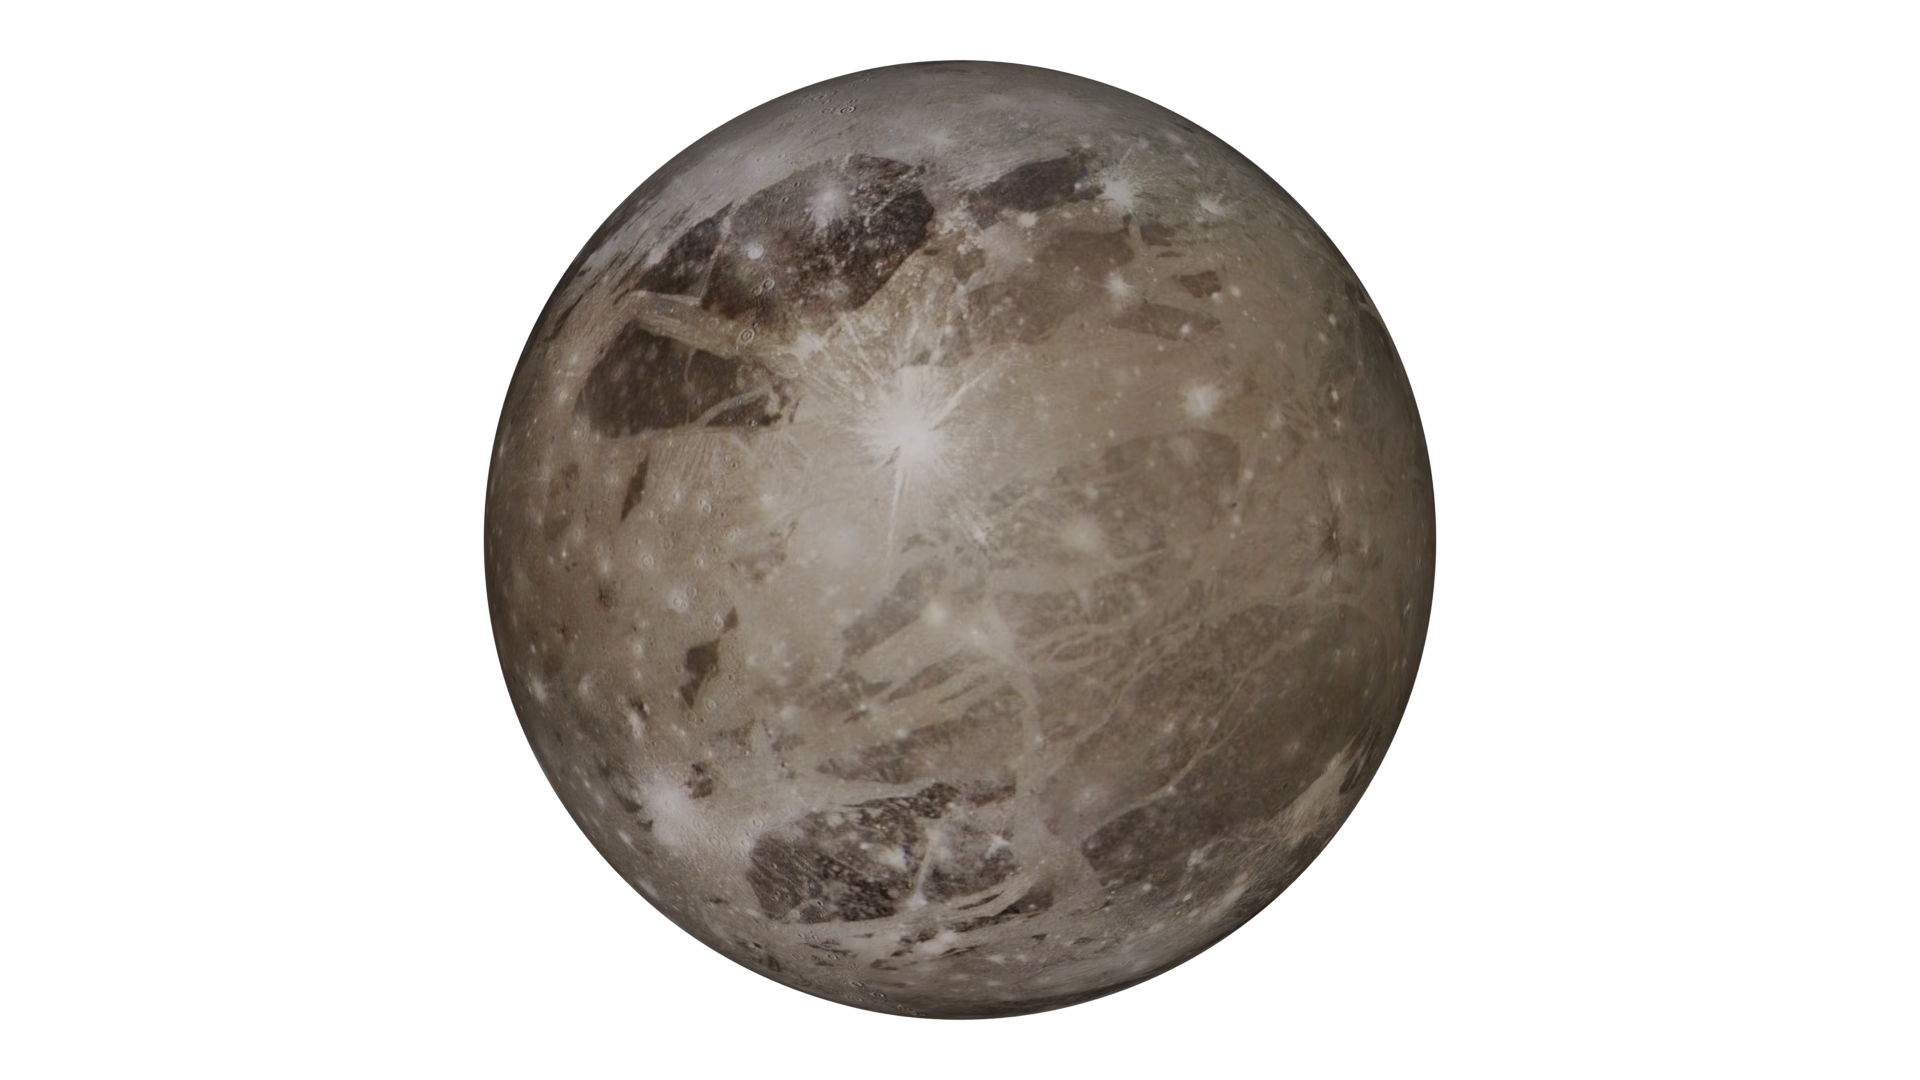
\includegraphics[width=\radpngL pt]{IMAGES/spheres/ganymede.png}};
		\end{scope}

	% The dashed lines in the front half of the white circle
	\begin{scope}
		\tdplotsetrotatedcoords{\Alpha}{0}{0}
		\path  [clip] 
			plot [domain=-90:90, samples=100] (cos \x, sin \x) 
			-- cycle;

		% Dashed light gray circle part 2
		\begin{scope}
		\tdplotsetrotatedcoords{\Alpha}{\Beta}{\Gamma}
		\draw  [behindline] 
			plot    [domain=0:360, samples=100] (cos \x, sin \x);
		\end{scope}

		\tdplotsetrotatedcoords{\Alpha-90}{-90}{90}
		\draw [behindline] (0,0) -- (cos \Beta, sin \Beta );

		\tdplotsetrotatedcoords{\Alpha}{\Beta}{\Gamma}
		\draw [behindline] (0,0,0) -- (1,0,0);

	\end{scope}

		
	% INERTIAL FRAME Axes
	\tdplotsetrotatedcoords{0}{0}{0}
	\draw[axis] (0,0,0) -- (0,-\L,0) node [anchor=north, xshift=0pt, yshift=-7pt]  {$\vec{e}_{1,\mathcal{P}}$};
	\draw[axis] (0,0,0) -- (\L,0,0) node [anchor=west, xshift=12pt, yshift=0pt] {$\vec{e}_{2,\mathcal{P}}$};
	\draw[axis] (0,0,0) -- (0,0,\L) node [anchor=north, xshift=7pt, yshift=+22pt] {$\vec{e}_{3,\mathcal{P}} \equiv \vec{p}$};

	% Laplace pole
	% \draw[axis] (0,0,0) -- (0,0,\Lnp) node [anchor=north, xshift=0pt, yshift=+22pt] {$\vec{p}$};

	% Orthogonal to the Line of NODES
	\tdplotsetrotatedcoords{\Alpha}{0}{0}
	\draw[axisint] (0,0,0) -- (1,0,0);
	\draw[behindline] (0,0,0) -- (-1,0,0); 

	% The BODY FIXED axes (care 1 and to are modified to compensate ZYZ to ZXZ order)
	\tdplotsetrotatedcoords{\Alpha}{\Beta}{\Gamma}
	\draw[axis] (0,0,0) -- (0,\L,0) node [anchor=north, xshift=10pt, yshift=20pt] {$\vec{e}_{1,\mathcal{B}}$};
	\draw[dashaxis] (0,0,0) -- (-\L,0,0) node [anchor=north, xshift=-22pt, yshift=13pt] {$\vec{e}_{2,\mathcal{B}}$};
	% \draw[axis] (0,0,0) -- (0,0,\L) node [anchor=east, xshift=-4pt, yshift=8pt] {$\vec{\omega}\vec{e}_{3,\mathcal{B}}$};
	\draw[axis] (0,0,0) -- (0,0,\L) node [anchor=north, xshift=-13pt, yshift=22pt] {$\vec{\omega} \approx \vec{e}_{3,\mathcal{B}} $};

	% Spin axis
	% \draw[axis] (0,0,0) -- (0,0,\Lnp) node [anchor=north, xshift=-6pt, yshift=20pt] {$\vec{\omega}$};

	
	% PHI
	\tdplotsetrotatedcoords{-90}{0}{0}
	\tdplotdrawarc[->]{(0,0,0)}{0.47}{0}{\Alphashift-1}{anchor=south, xshift=0pt, yshift=-13pt}{$\varphi^\prime$}
	% PSI
	\tdplotsetrotatedcoords{\Alpha}{\Beta}{\Gamma}
	\tdplotdrawarc[->]{(0,0,0)}{0.47}{90-\Gamma}{90}{anchor=south, xshift=7pt, yshift=-14pt}{$\psi^\prime$}
	% THETA (between BF axes)
	\tdplotsetrotatedcoords{\Alpha+90}{90}{0}
	\tdplotdrawarc[->]{(0,0,0)}{0.75}{-180}{-180+\Beta}{anchor=south, xshift=-1pt, yshift=0pt}{$\theta^\prime$}
	% THETA (dark sector)
	\tdplotsetrotatedcoords{\Alpha+90}{90}{0}
	\tdplotdrawarc[->, dashed]{(0,0,0)}{.75}{-90}{-90+\Beta}{anchor=south, xshift=-8pt, yshift=-12pt}{$\theta^\prime$}


	% % SNK vectors
	% \def\Lsnk{1.33*\L}

	% % S: spin
	% \tdplotsetrotatedcoords{\Alpha}{\Beta}{\Gamma}
	% \draw[axis] (0,0,0) -- (0,0,\Lsnk) node [anchor=east, xshift=-3pt, yshift=12pt] {$\vec{\omega}$};
	% % K: Laplace plane vector
	% \def\incl{10}
	% \tdplotsetrotatedcoords{\Alpha}{\Beta+\incl}{\Gamma}
	% \draw[axis] (0,0,0) -- (0,0,\Lsnk) node [anchor=east, xshift=-7pt, yshift=9pt] {$\vec{p}$};
	% % N: Orbit normal
	% \def\eps{5}
	% \tdplotsetrotatedcoords{\Alpha}{\Beta+\eps}{\Gamma}
	% \draw[axis] (0,0,0) -- (0,0,\Lsnk) node [anchor=east, xshift=-5pt, yshift=12pt] {$\vec{n}$};

	% % EPSILON: obliquity arc
	% \tdplotsetrotatedcoords{\Alpha+90}{90}{0}
	% \tdplotdrawarc[->]{(0,0,0)}{0.8}{-180+\Beta}{-180+\Beta + \eps}{anchor=south, xshift=-5pt, yshift=0pt}{$\epsilon$}

	% % I: incl arc
	% \tdplotsetrotatedcoords{\Alpha+90}{90}{0}
	% \tdplotdrawarc[->]{(0,0,0)}{0.88}{-180+\Beta+\eps}{-180+\Beta + \incl}{anchor=south, xshift=-5pt, yshift=-2pt}{$i$}

	% Arrows angles
	% PHI
	%\tdplotsetrotatedcoords{0}{0}{0}
	% \tdplotdrawarc[->, dashed]{(0,0,0)}{0.69}{0}{\Alphashift-1}{anchor=south, xshift=7pt, yshift=-4pt}{$\varphi$}

	% \tdplotsetrotatedcoords{\Alpha+90}{90}{0}
	% \tdplotdrawarc[->]{(0,0,0)}{.75}{-90}{-90+\Beta}{anchor=south, xshift=-6pt, yshift=-10pt}{$\theta$}

	% new theta
	% \tdplotsetrotatedcoords{\Alpha+90}{90}{0}
	% \tdplotdrawarc[->]{(0,0,0)}{0.8}{90}{90+\Beta}{left}{$\theta$}

	% \tdplotsetrotatedcoords{\Alpha}{\Beta}{\Gamma}
	% \tdplotdrawarc[->]{(0,0,0)}{0.8}{-\Gamma}{0}{below}{$\psi$}


	\end{scope}

	\end{tikzpicture}

	
	% \caption{
	% Schematic representation of the relations between the Euler angles, the space-fixed frame ${\mathcal{I}}$ centered on the satellite and the satellite's principal axis frame 
	% ${\mathcal{B}}$.
	% }

	% and the inertially fixed Laplace plane normal $\vec{p}$. %quasi-inertial
	\label{fig:tikz_euler}
	\end{subfigure}
	% <-- important to keep both figure in the same line
	%_____________________________________________________________
	%									FIGURE: ORBITAL ELEMENTS
	%_____________________________________________________________
	\begin{subfigure}[t]{0.495\textwidth}
	\centering

	\def\radius{3.5}
	\def\Alpha{180 + 32} %28
	\def\Alphashift{\Alpha-180}
	\def\Beta{25}
	\def\Gamma{100}

	\def\L{1}
	\def\Lnp{1}

	\def\radpngL{50}
	\def\radpngM{35}

	\tdplotsetmaincoords{70}{-7}

	\tikzset{% Some styles
		axisint/.style={thin, -},
		axis/.style={thin, fill=black, -latex', shorten >=-10pt},
		dashaxis/.style={thin, fill=black, -latex', shorten >=-10pt, loosely dashed},
		behindline/.style={loosely dashed}
	}


	\begin{tikzpicture}[tdplot_main_coords, scale=\radius]

	\begin{scope}[every path/.style={tdplot_rotated_coords}]

	% Back half of the white circle.
	\tdplotsetrotatedcoords{\Alpha}{0}{0}
	\draw  [fill=white] 
		plot    [domain=90:270, samples=100] (cos \x, sin \x) -- cycle;

	% Dark gray circle
	\tdplotsetrotatedcoords{\Alpha+90}{90}{90}
	\draw [fill=gray!80, thin, domain=0:\Beta] 
		(0,0) -- plot (cos \x, sin \x) -- cycle;

	% The light gray circle
	\tdplotsetrotatedcoords{\Alpha}{\Beta}{\Gamma}
	\draw  [fill=gray!20] 
		plot    [domain=0:360, samples=100] (cos \x, sin \x);


	% The dashed edge of the back half of the white circle
	\begin{scope}
	\tdplotsetrotatedcoords{\Alpha}{\Beta}{\Gamma}
	\path  [clip] 
		plot    [domain=0:360, samples=100] (cos \x, sin \x);

	\tdplotsetrotatedcoords{\Alpha}{0}{0}
	\draw  [behindline] 
		plot    [domain=90:270, samples=100] (cos \x, sin \x);

	\end{scope}

	% The dark gray sector
	\tdplotsetrotatedcoords{\Alpha-90}{-90}{90}
	\draw [fill=gray!80, thin, domain=0:\Beta] 
		(0,0) -- plot (cos \x, sin \x) -- cycle;

	% Dashed light gray circle part 1
	\begin{scope}
	\tdplotsetrotatedcoords{\Alpha}{\Beta}{\Gamma}
	\draw  [behindline] 
		plot    [domain=0:360, samples=100] (cos \x, sin \x);
	\end{scope}

	% THETA (dark gray arc)
	\tdplotsetrotatedcoords{\Alpha+90}{90}{0}
	\tdplotdrawarc[->]{(0,0,0)}{.75}{-90}{-90+\Beta}{anchor=south, xshift=-6pt, yshift=-10pt}{}

	% The front half of the WHITE circle
	\tdplotsetrotatedcoords{\Alpha}{0}{0}  
	\draw  [fill=white] 
		plot [domain=-90:90, samples=100] (cos \x, sin \x) 
		-- cycle;


	% Line of NODES
	\draw[axis] (0,0,0) -- (0,\L,0) node [anchor=west, xshift=7pt, yshift=-7pt] {$\vec{N}$};


	% SMALL SPHERE (Jupiter)
	%\shade[tdplot_screen_coords, ball color=brown!50] (0,0) circle (2pt);
	% Image overlay clipped in circle
	\begin{scope}[tdplot_screen_coords]
	%\clip (0,0) circle (10pt); % match circle size
	\node at (0,0) {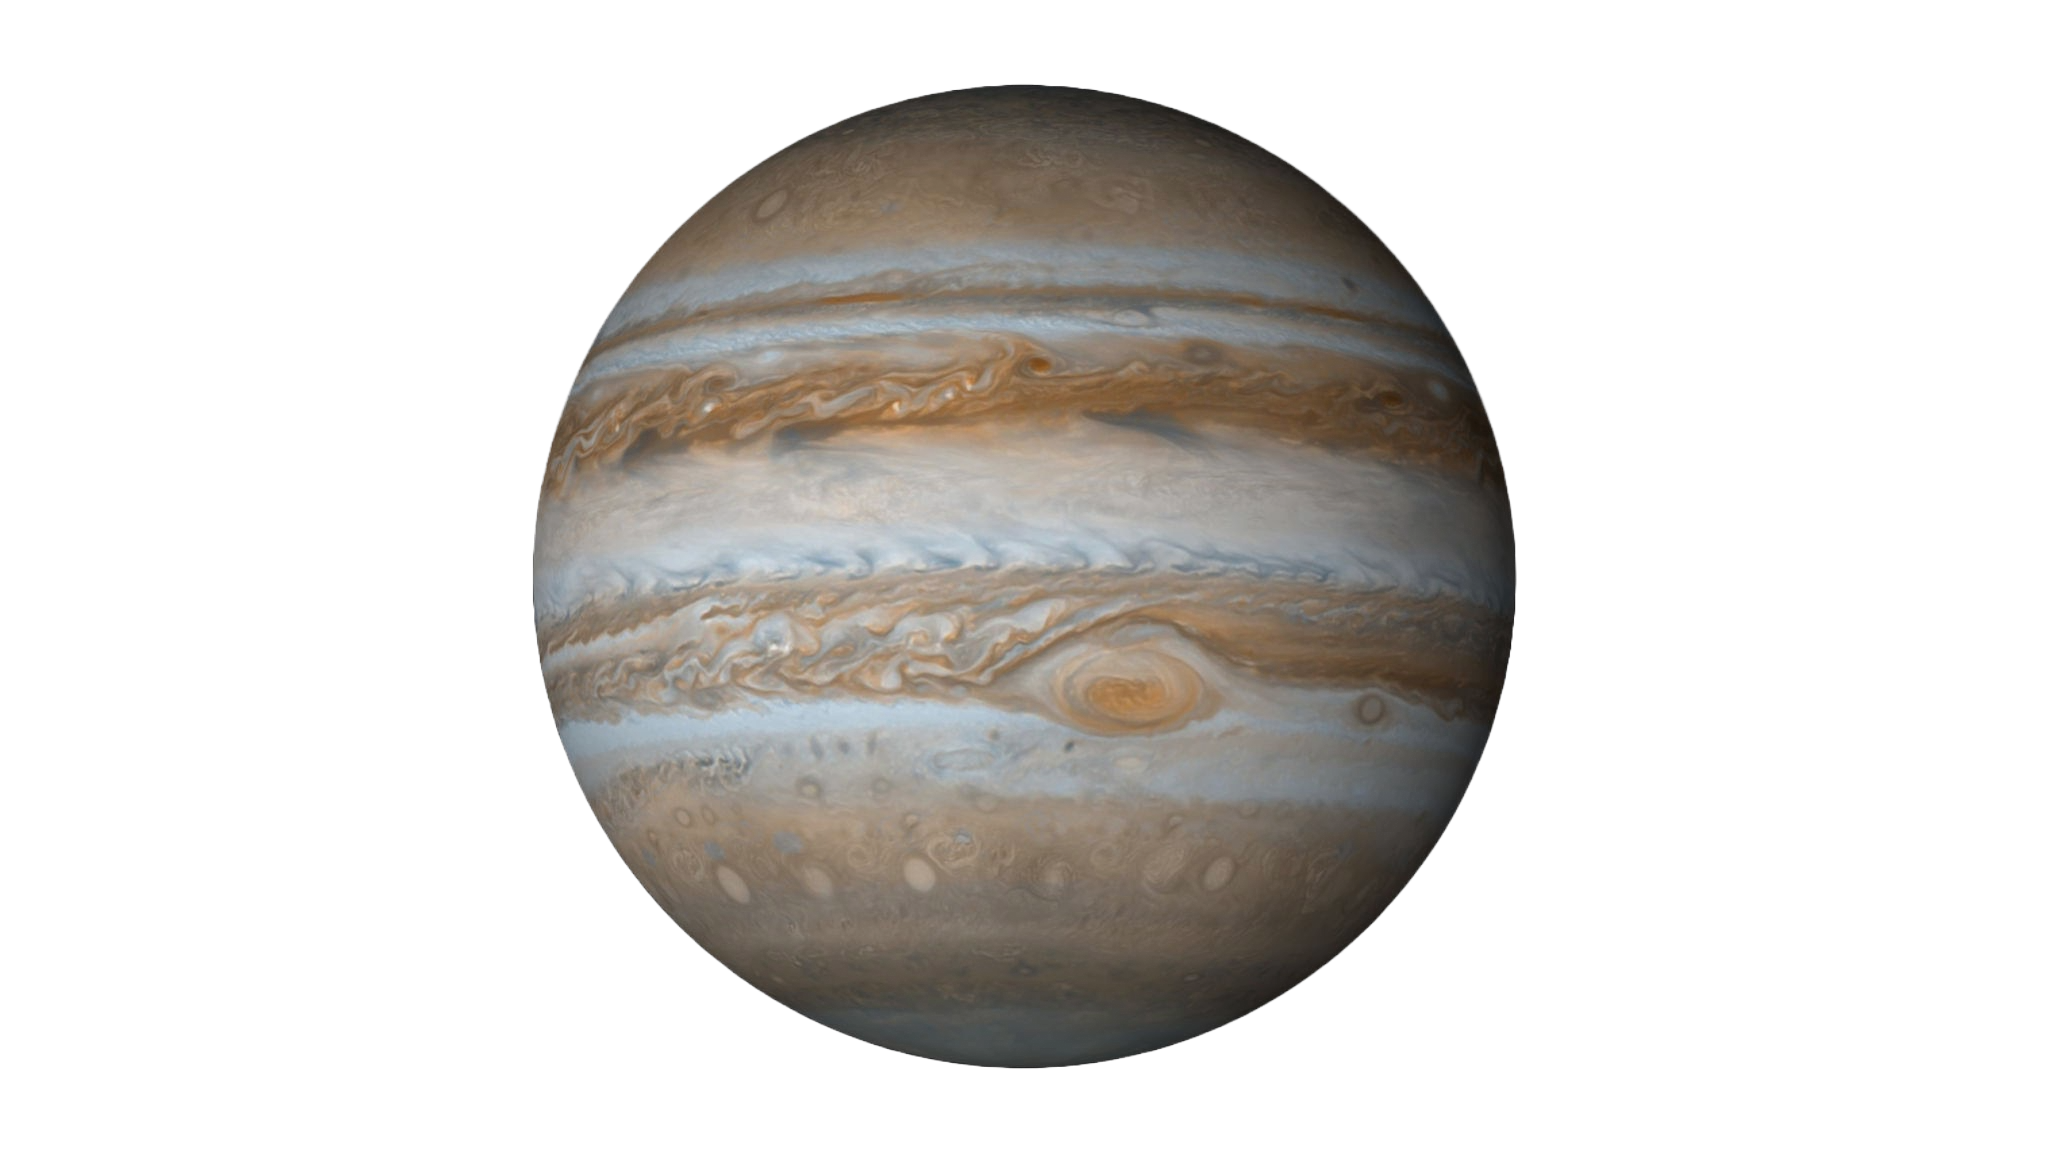
\includegraphics[width=\radpngL pt]{IMAGES/spheres/jupiter.png}};
	\end{scope}

	% The dashed lines in the front half of the white circle
	\begin{scope}
		\tdplotsetrotatedcoords{\Alpha}{0}{0}
		\path  [clip] 
			plot [domain=-90:90, samples=100] (cos \x, sin \x) 
			-- cycle;


		% Dashed light gray circle part 2
		\begin{scope}
		\tdplotsetrotatedcoords{\Alpha}{\Beta}{\Gamma}
		\draw  [behindline] 
			plot    [domain=0:360, samples=100] (cos \x, sin \x);
		\end{scope}


		\tdplotsetrotatedcoords{\Alpha-90}{-90}{90}
		\draw [behindline] (0,0) -- (cos \Beta, sin \Beta );

		\tdplotsetrotatedcoords{\Alpha}{\Beta}{\Gamma}
		\draw [behindline] (0,0,0) -- (1,0,0);

	\end{scope}

		
	% INERTIAL FRAME Axes
	\tdplotsetrotatedcoords{0}{0}{0}
	\draw[axis] (0,0,0) -- (0,-\L,0) node [anchor=north, xshift=0pt, yshift=-7pt]  {$\vec{e}_{1,\mathcal{P}}$};
	\draw[axis] (0,0,0) -- (\L,0,0) node [anchor=west, xshift=12pt, yshift=0pt] {$\vec{e}_{2,\mathcal{P}}$};
	\draw[axis] (0,0,0) -- (0,0,\L) node [anchor=north, xshift=7pt, yshift=+22pt] {$\vec{e}_{3,\mathcal{P}} \equiv \vec{p}$};

	% Laplace pole
	% \draw[axis] (0,0,0) -- (0,0,\Lnp) node [anchor=north, xshift=0pt, yshift=+22pt] {$\vec{p}$};


	% Orthogonal to the Line of NODES
	\tdplotsetrotatedcoords{\Alpha}{0}{0}
	\draw[axisint] (0,0,0) -- (\L,0,0);
	\draw[behindline] (0,0,0) -- (-\L,0,0); 
	% Line of NODES (dashed)
	%\draw[behindline] (0,-\L,0) -- (0,\L,0);

	% The BODY FIXED axes (care 1 and to are modified to compensate ZYZ to ZXZ order)
	\tdplotsetrotatedcoords{\Alpha}{\Beta}{\Gamma}

	% SMALL SPHERE (Ganymede)
	\begin{scope}[tdplot_main_coords]
		% Sphere at (0, \L, 0)
		%\shade[ball color=brown!50] (0,\L,0) circle (2pt);

		% Image texture clipped to circle, at same 3D location
		\begin{scope}
			\path (0,\L,0) coordinate (spherepos);
			\begin{scope}[shift={(spherepos)}]
				%\clip (0,0) circle (10pt); % match circle radius
				\node at (0,0) {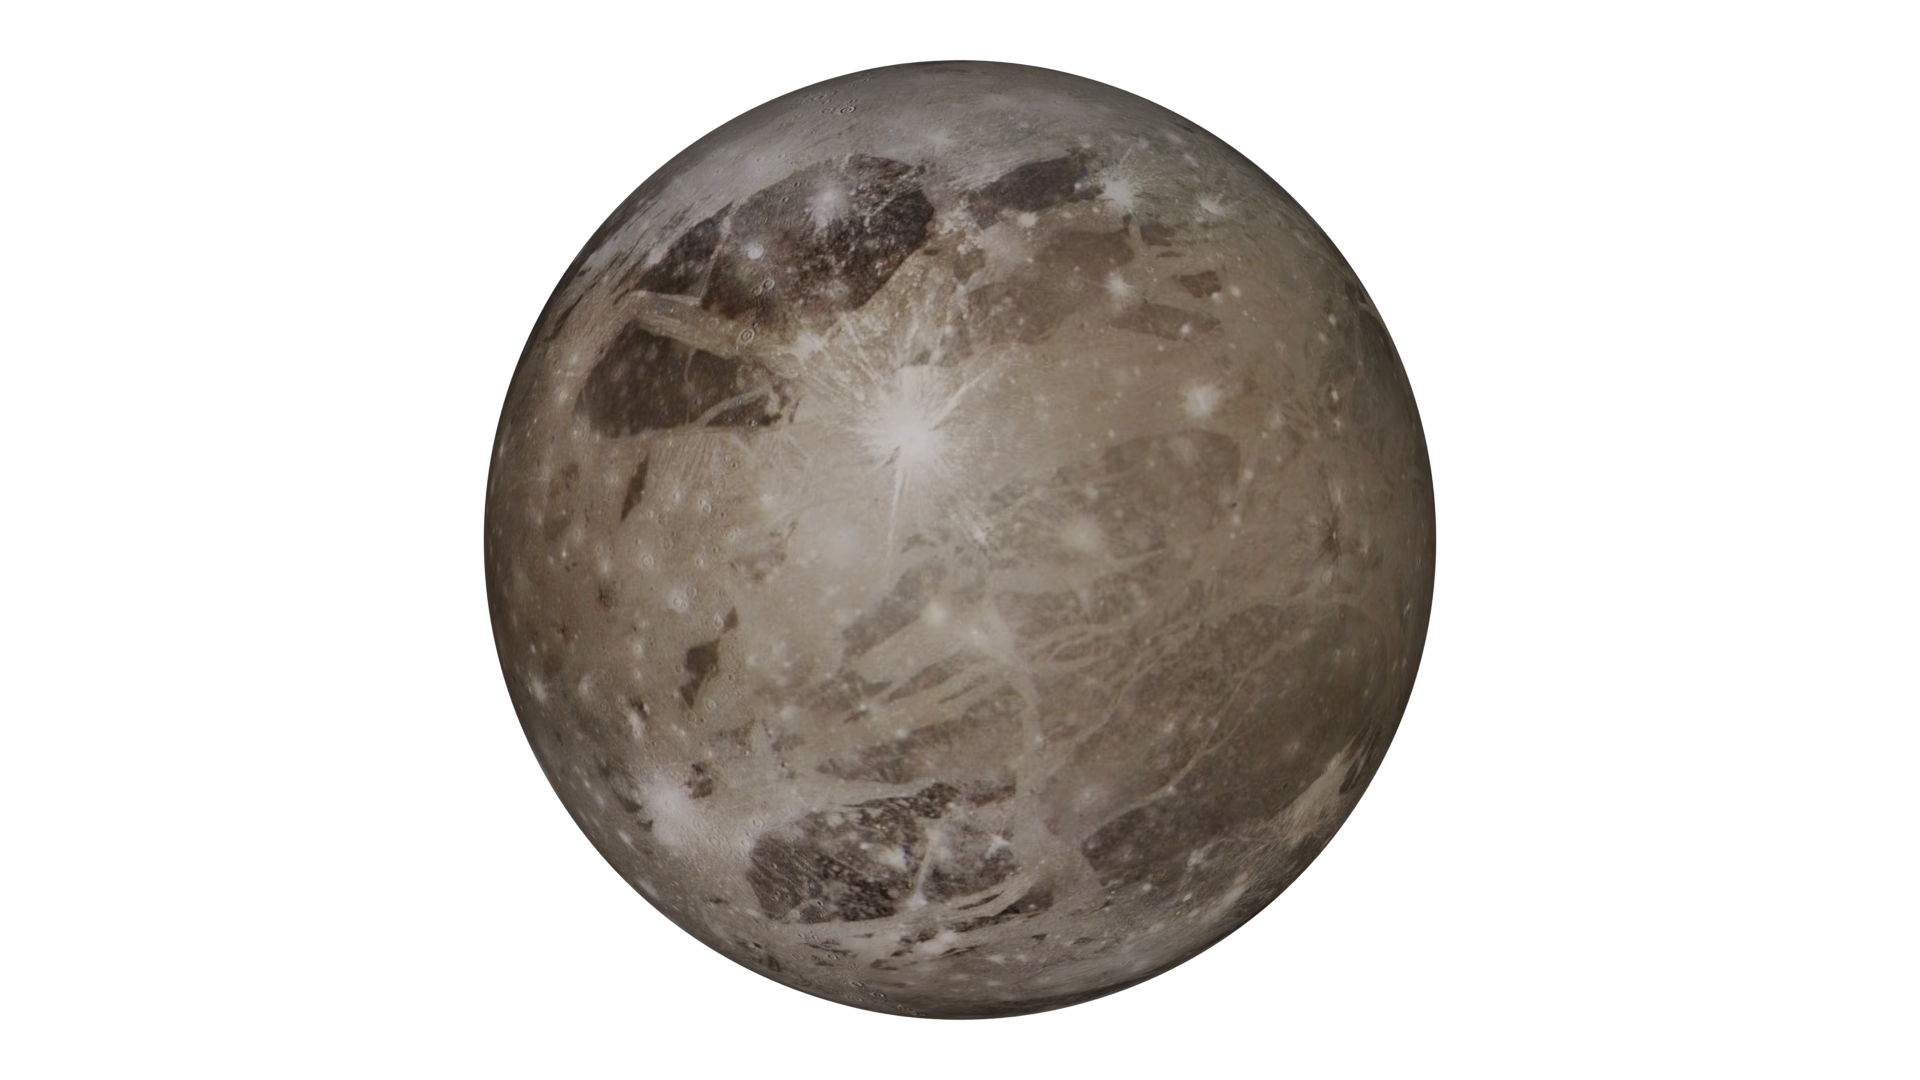
\includegraphics[width=\radpngM pt]{IMAGES/spheres/ganymede.png}};
			\end{scope}
		\end{scope}
		\draw  [dashed] 
		plot    [domain=20:120, samples=100] (cos \x, sin \x);
	\end{scope}

	

	% Principal frame axes 
	\path (0,\L,0) coordinate (spherepos);
	\begin{scope}[tdplot_rotated_coords, shift={(spherepos)}]
	\draw[axis] (0,0,0) -- (0,-.1*\L,0) node [anchor=north, xshift=0pt, yshift=-5pt]  {$\vec{e}_{1,\mathcal{B}}$};
	\draw[axis] (0,0,0) -- (.1*\L,0,0) node [anchor=west, xshift=10pt, yshift=-3pt] {$\vec{e}_{2,\mathcal{B}}$};
	\draw[axis] (0,0,0) -- (0,0,.1*\L) node [anchor=north, xshift=-2pt, yshift=+22pt] {$\vec{e}_{3,\mathcal{B}}$};
	\end{scope}

	% Orbit normal
	\draw[axisint] (0,0,0) -- (0,\L,0) node [anchor=north, xshift=7pt, yshift=22pt] {};
	\draw[behindline] (0,0,0) -- (-\L,0,0) node [anchor=north, xshift=-22pt, yshift=14pt] {};
	\draw[axis] (0,0,0) -- (0,0,\Lnp) node [anchor=north, xshift=-7pt, yshift=22pt] {$\vec{n}$};
	
	% \Omega: longitude of the ascending node
	\tdplotsetrotatedcoords{-90}{0}{0}
	\tdplotdrawarc[->]{(0,0,0)}{0.47}{0}{\Alphashift-1}{anchor=south, xshift=3pt, yshift=-14pt}{$\Omega$}
	% u: argument of latitude
	\tdplotsetrotatedcoords{\Alpha}{\Beta}{\Gamma}
	\tdplotdrawarc[->]{(0,0,0)}{0.47}{90-\Gamma}{90}{anchor=south, xshift=7pt, yshift=-12pt}{$u$}

	% \varpi: longitude of pericenter
	% \tdplotdrawarc[->]{(0,0,0)}{0.32}{90-\Gamma}{\wperi}{anchor=south, xshift=7pt, yshift=-12pt}{$\omega$}

	% i (between BF axes)
	\tdplotsetrotatedcoords{\Alpha+90}{90}{0}
	\tdplotdrawarc[->]{(0,0,0)}{0.75}{-180}{-180+\Beta}{anchor=south, xshift=-1pt, yshift=0pt}{$i$}
	% i (dark sector)
	\tdplotsetrotatedcoords{\Alpha+90}{90}{0}
	\tdplotdrawarc[->, dashed]{(0,0,0)}{.75}{-90}{-90+\Beta}{anchor=south, xshift=-8pt, yshift=-12pt}{$i$}

	\end{scope}


	% % \varpi: argument of pericenter
	% \def\wperi{20}
	% \tdplotsetrotatedcoords{\Alpha}{\Beta}{\Gamma + \wperi}
	% \begin{scope}[tdplot_rotated_coords]
	% 	% peripasis?'
	% 	\draw[axisint] (0,0,0) -- (0,\L,0) node [anchor=north, xshift=7pt, yshift=22pt] {};
	% 	\draw[behindline] (0,0,0) -- (0,-\L,0) node [anchor=north, xshift=7pt, yshift=22pt] {};
	% 	\tdplotdrawarc[->]{(0,0,0)}{0.32}{90-\Gamma - \wperi}{90}{anchor=south, xshift=4pt, yshift=0pt}{$\omega$}
	% \end{scope}

	%     \shade[ball color=brown!50] (0,\L,0) circle (2pt); % sphere at tip of p
	% 	\clip (0,0) circle (10pt); % match circle size
	% 	\node at (0,0) {
\includegraphics[width=25pt]{IMAGES/ganymede.png}};
	% \draw  [dashed] 
	%     plot    [domain=20:120, samples=100] (cos \x, sin \x);
	% \end{scope}

	% \tdplotsetrotatedcoords{\Alpha+90}{90}{0}
	% \tdplotdrawarc[->]{(0,0,0)}{.75}{-90}{-90+\Beta}{anchor=south, xshift=-6pt, yshift=-10pt}{$\theta$}
	% new theta
	% \tdplotsetrotatedcoords{\Alpha+90}{90}{0}
	% \tdplotdrawarc[->]{(0,0,0)}{0.8}{90}{90+\Beta}{left}{$\theta$}
	% \tdplotsetrotatedcoords{\Alpha}{\Beta}{\Gamma}
	% \tdplotdrawarc[->]{(0,0,0)}{0.8}{-\Gamma}{0}{below}{$\psi$}

	% % The BODY FIXED axes (care 1 and to are modified to compensate ZYZ to ZXZ order)
	% \tdplotsetrotatedcoords{\Alpha}{\Beta}{\Gamma}
	% \draw[axis] (0,0,0) -- (0,\L,0) node [anchor=north, xshift=7pt, yshift=22pt] {$\vec{e}_{1,\mathcal{B}}$};
	% \draw[dashaxis] (0,0,0) -- (-\L,0,0) node [anchor=north, xshift=-22pt, yshift=14pt] {$\vec{e}_{2,\mathcal{B}}$};
	% \draw[axis] (0,0,0) -- (0,0,\L) node [anchor=north, xshift=5pt, yshift=20pt] {$\vec{e}_{3,\mathcal{B}}$};

	% % SNK vectors
	% \def\Lsnk{1.33*\L}

	% % S: spin
	% \tdplotsetrotatedcoords{\Alpha}{\Beta}{\Gamma}
	% \draw[axis] (0,0,0) -- (0,0,\Lsnk) node [anchor=east, xshift=-3pt, yshift=12pt] {$\vec{\omega}$};
	% % K: Laplace plane vector
	% \def\incl{10}
	% \tdplotsetrotatedcoords{\Alpha}{\Beta+\incl}{\Gamma}
	% \draw[axis] (0,0,0) -- (0,0,\Lsnk) node [anchor=east, xshift=-7pt, yshift=9pt] {$\vec{p}$};
	% % N: Orbit normal
	% \def\eps{5}
	% \tdplotsetrotatedcoords{\Alpha}{\Beta+\eps}{\Gamma}
	% \draw[axis] (0,0,0) -- (0,0,\Lsnk) node [anchor=east, xshift=-5pt, yshift=12pt] {$\vec{n}$};

	% % EPSILON: obliquity arc
	% \tdplotsetrotatedcoords{\Alpha+90}{90}{0}
	% \tdplotdrawarc[->]{(0,0,0)}{0.8}{-180+\Beta}{-180+\Beta + \eps}{anchor=south, xshift=-5pt, yshift=0pt}{$\epsilon$}

	% % I: incl arc
	% \tdplotsetrotatedcoords{\Alpha+90}{90}{0}
	% \tdplotdrawarc[->]{(0,0,0)}{0.88}{-180+\Beta+\eps}{-180+\Beta + \incl}{anchor=south, xshift=-5pt, yshift=-2pt}{$i$}

	% Arrows angles
	% PHI
	%\tdplotsetrotatedcoords{0}{0}{0}
	% \tdplotdrawarc[->, dashed]{(0,0,0)}{0.45}{0}{\Alphashift-1}{anchor=south, xshift=7pt, yshift=-4pt}{}%{$\Omega$}

	
	

	\end{tikzpicture}

	% \caption{
	% Schematic representation of the orbital elements. The origin of the $\mathcal{P}$ frame here has been translated on Jupiter for illustrative purposes.
	% }

	% and the inertially fixed Laplace plane normal $\vec{p}$. %quasi-inertial
	\label{fig:tikz_orbital}
	\end{subfigure}

\caption{In the left panel we show a schematic representation of the relations between the Euler angles, the space-fixed Laplace frame ${\mathcal{P}}$ and the satellite's principal axis frame 
${\mathcal{B}}$.
On the right, we show a 
schematic representation of the relationship between the orbit, and the orientation of these reference frames. 
%Longitude of the ascending node ($\Omega)$, the argument of latitude ($u$). 
The origin of the $\mathcal{P}$ frame in the right panel has been translated on Jupiter for illustrative purposes.
}
\label{fig:tikz_orbital_euler}
\end{figure*}
%_____________________________________________________________

% %_____________________________________________________________
% % 							FIGURE: Cassini states I and II
% %_____________________________________________________________
% \begin{figure}
% 	\centering
% 	\tdplotsetmaincoords{78}{-160} % 3D view angle: {elevation}{azimuth}
% 	%_____________________________________________________________
% 	% 											CASSINI STATE I
% 	%_____________________________________________________________
% 	\begin{subfigure}[t]{0.24\textwidth}
% 		\centering %\raggedright
		
% 		\begin{tikzpicture}[tdplot_main_coords, scale=4, line cap=round,
% 		axis/.style={thin, fill=black, -latex', shorten >=-7pt},
% 		dashaxis/.style={thin, fill=black, -latex', shorten >=-7pt, dashed},
% 		blackline/.style={thin, fill=black},
% 		dashline/.style={thin, fill=black, dashed}]
% 		% ---- PARAMETERS ----
% 		\def\L{1.0}     % Length of vectors (unit length)
% 		\def\inc{16}    % Inclination angle of n (degrees)
% 		\def\eps{\inc-5}    % Angle between n and s (degrees) < incl
% 		\def\r{0.15}    % Radius of precession circles
% 		\def\azn{45}    % Azimuth angle of n (degrees)
% 		\def\azs{\azn}    % Azimuth angle of s (degrees)

% 		\def\prec{70}
% 		\def\psioffset{70}
% 		\def\radep{2.2*\r}

% 		\def\arrangnzero{148} % angle start of the circle arrow
% 		\def\arrangszero{140} % angle start of the circle arrow
% 		\def\arrangn{352} % angle swiped by the circle arrow
% 		\def\arrangs{355} % angle swiped by the circle arrow

% 		\def\KtoS{\eps+\inc}

% 		\def\radpngS{27}

% 		% ---- COORDINATES ----
% 		\coordinate (O) at (0,0,0); % Origin
% 		\coordinate (K) at (0,0,\L);  % Laplace plane unit vector

% 		% The white circle (LAPLACE PLANE) part 1
% 		\tdplotsetrotatedcoords{\prec}{0}{0}
% 		\begin{scope}[tdplot_rotated_coords]
% 		\draw[fill=white] 
% 			plot [domain=0:360, samples=100] ({\radep * cos(\x)}, {\radep * sin(\x)});
% 		\draw[axis] (0,0,0) -- (\radep,0,0); %node [anchor=west, xshift=-25pt, yshift=0pt] {$\vec{e}_{1,\mathcal{P}}$};
% 		\draw[axis] (0,0,0) -- (0,\radep,0); % node [anchor=north, xshift=20pt, yshift=5pt] {$\vec{e}_{2,\mathcal{P}}$};
% 		\draw[axis] (0,0,0) -- (0,0,\radep); % node [anchor=west, xshift=-25pt, yshift=0pt] {$\vec{e}_{3,\mathcal{P}}$};
% 		\end{scope}


% 		% Orbit normal vector \vec{n} = inclined by \inc from z-axis with azimuth \azn
% 		\coordinate (N) at ({\L*sin(\inc)*cos(\azn)},{\L*sin(\inc)*sin(\azn)},{\L*cos(\inc)});

% 		% Spin vector \vec{\omega} = inclined by \inc+\eps from z-axis with azimuth \azs
% 		\coordinate (S) at ({\L*sin(\inc + \eps)*cos(\azs)},{\L*sin(\inc + \eps)*sin(\azs)},{\L*cos(\inc + \eps)});

% 		% Circle centers at tips of vectors projected to z=\L plane
% 		\coordinate (ON) at (0,0,{\L*cos(\inc)}); 
% 		\coordinate (OS) at (0,0,{\L*cos(\inc + \eps)});   

% 		% Circle radii
% 		\pgfmathsetmacro{\rn}{sqrt((\L*sin(\inc)*cos(\azn))^2 + (\L*sin(\inc)*sin(\azn))^2)}
% 		\pgfmathsetmacro{\rs}{sqrt((\L*sin(\inc + \eps)*cos(\azs))^2 + (\L*sin(\inc + \eps)*sin(\azs))^2)}

% 		% GRAY CIRCLE (EQUATORIAL PLANE)
% 		\tdplotsetrotatedcoords{\azs}{\KtoS}{0}
% 		\begin{scope}[tdplot_rotated_coords]
% 		\draw[fill=gray!20] 
% 			plot [domain=0:360, samples=100] ({\radep * cos(\x)}, {\radep * sin(\x)});

	
% 		% NODE LINE (dashed)
% 		\draw[dashline] (0,0,0) -- (0,-\radep,0);
% 		\draw[dashline] (0,0,0) -- (0,\radep,0);

% 		\end{scope}

% 		% The front half of the WHITE circle
% 		\tdplotsetrotatedcoords{\azs}{0}{0}  
% 		\begin{scope}[tdplot_rotated_coords]
% 		\draw  [fill=white] 
% 			plot [domain=-90:90, samples=100] (\radep * cos \x, \radep * sin \x) 
% 			-- cycle;
% 		\end{scope}

% 		% SMALL SPHERE
% 		\shade[tdplot_screen_coords, ball color=brown!50] (0,0) circle (1.5pt);
% 		% Image overlay clipped in circle
% 		\begin{scope}[tdplot_screen_coords]
% 		%\clip (0,0) circle (1.5pt); % match circle size
% 		\node at (0,0) {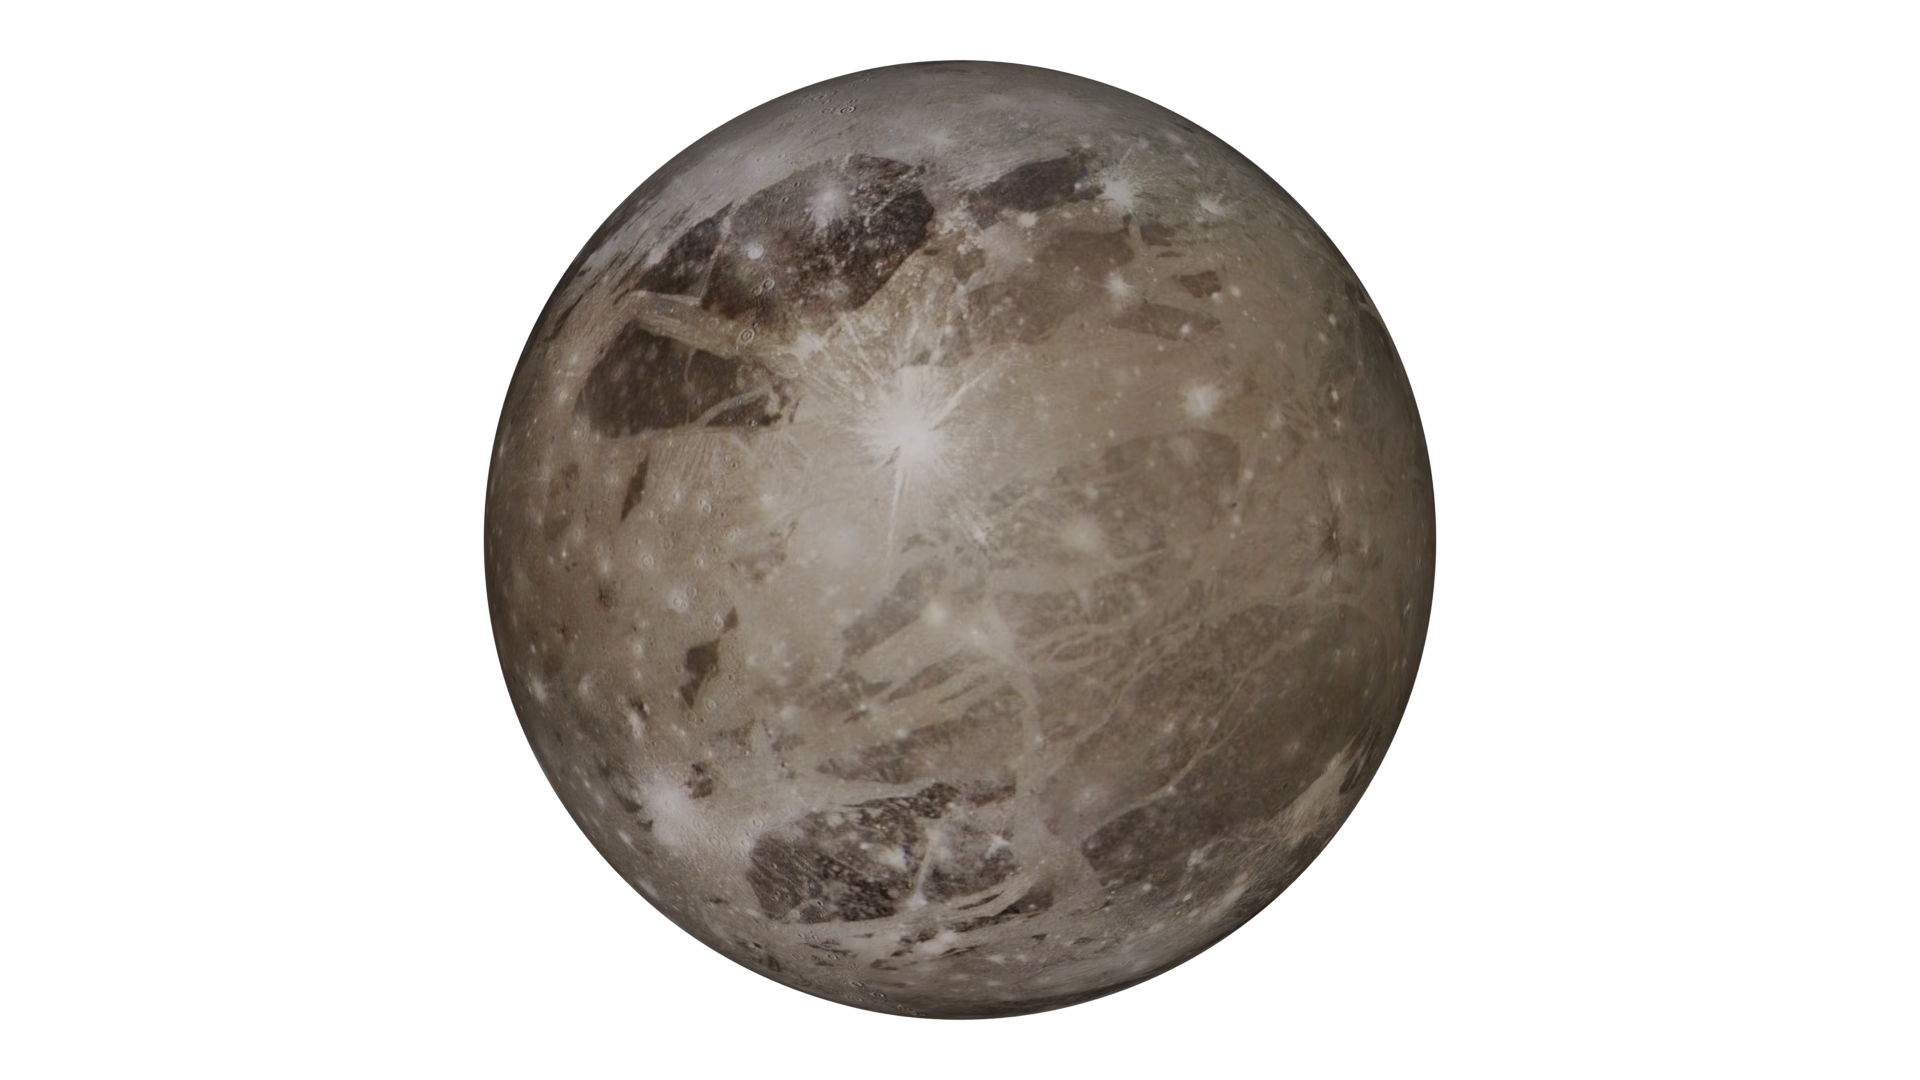
\includegraphics[width=\radpngS pt]{IMAGES/spheres/ganymede.png}};
% 		\end{scope}


% 		\tdplotsetrotatedcoords{\azs}{\KtoS}{\psioffset}
% 		\begin{scope}[tdplot_rotated_coords]
% 		\draw[axis] (0,0,0) -- (\radep,0,0) node [anchor=north, xshift=1pt, yshift=-5pt] {$\vec{e}_{1,\mathcal{B}}$};
% 		\draw[axis] (0,0,0) -- (0,\radep,0) node [anchor=west, xshift=5pt, yshift=5pt] {$\vec{e}_{2,\mathcal{B}}$};
% 		\draw[axis] (0,0,0) -- (0,0,\radep) node [anchor=west, xshift=-25pt, yshift=0pt] {$\vec{e}_{3,\mathcal{B}}$};
% 		\end{scope}

% 		% % The light gray circle (EQUATORIAL PLANE)
% 		% \tdplotsetrotatedcoords{\azs}{\KtoS}{0}
% 		% \def\radep{2*\r}
% 		% \draw  [tdplot_rotated_coords, fill=gray!20] 
%    		%  plot [domain=0:360, samples=100] ({\radep * cos(\x)}, {\radep * sin(\x)});
% 		% % The BODY FIXED axes
% 		% \draw[axis] (0,0,0) -- (\radep,0,0) node [anchor=north, xshift=-20pt, yshift=12pt] {$\vec{e}_{1,\mathcal{B}}$};
% 		% \draw[axis] (0,0,0) -- (0,\radep,0) node [anchor=north, xshift=5pt, yshift=18pt] {$\vec{e}_{2,\mathcal{B}}$};
% 		% \draw[axis] (0,0,0) -- (0,0,\radep) node [anchor=north, xshift=5pt, yshift=20pt] {$\vec{e}_{3,\mathcal{B}}\approx \vec{\omega}$};



% 		% ---- PRECESSION CIRCLES ----
% 		%Circle around tip of \vec{\omega} (filled white with solid line)
% 		\tdplotdrawarc[
% 			tdplot_main_coords,
% 			white,
% 			thin,
% 			fill=white
% 		]{(OS)}{\rs}{0}{360}{}{}
		
% 		% Arrow on s-circle (clockwise)
% 		\tdplotdrawarc[
% 			tdplot_main_coords,
% 			black,
% 			thin,
% 			->
% 		]{(OS)}{\rs}{\arrangszero}{\arrangszero-\arrangs}{anchor=south west, xshift=51pt, yshift=-35pt}{$\dot{\varphi}^\prime$}
% 		% syntax:  {}{}{start angle}{end angle} 
% 		% set start angle > end angle for clockwise arrow 

% 		%Circle around tip of \vec{n} (filled white with solid line)
% 		\tdplotdrawarc[
% 			tdplot_main_coords,
% 			white,
% 			thin,
% 			fill=white
% 		]{(ON)}{\rn}{0}{360}{}{}
		
% 		% Arrow on n-circle (clockwise)
% 		\tdplotdrawarc[
% 			tdplot_main_coords,
% 			black,
% 			thin,
% 			->
% 		]{(ON)}{\rn}{\arrangnzero}{\arrangnzero-\arrangn}{}{}

% 		% DASHED circle precession
% 		%Circle around tip of \vec{\omega} (filled white with solid line)
% 		\tdplotdrawarc[
% 			tdplot_main_coords,
% 			black,
% 			loosely dashed,
% 		]{(OS)}{\rs}{0}{360}{}{}

% 		% ---- VECTORS ----
% 		% Reference axis \vec{p} (aligned with z)
% 		\draw[->, -latex', black, thin] (O) -- (K)
% 			node[above, xshift=0pt, yshift=2pt] {${\vec{p}}$};

% 		% Orbit normal \vec{n}
% 		\draw[->, -latex', black, thin] (O) -- (N)
% 			node[left, xshift=0pt, yshift=-3pt] {${\vec{n}}$};

% 		% Spin axis \vec{\omega}
% 		\draw[->, -latex', black, thin] (O) -- (S)
% 			node[left, xshift=-0.0pt, yshift=-3pt] {${\vec{\omega}}$};

% 		% ---- ANGLE ARCS ----
% 		% INCLINATION: Angle between k and n (\inc) - label changed to \theta
% 		\tdplotsetthetaplanecoords{\azn}
% 		\tdplotdrawarc[
% 			tdplot_rotated_coords,
% 			black,
% 			thin,
% 			->,
% 		]{(O)}{0.50}{0}{\inc}{anchor=south west, xshift=-5pt, yshift=1pt}{$i$} % syntax: {}{height?}{}{}{label}

% 		\tdplotdrawarc[
% 			tdplot_rotated_coords,
% 			black,
% 			thin,
% 			->,
% 		]{(O)}{0.65}{0}{\inc+\eps}{anchor=south west, xshift=-4pt, yshift=1pt}{${\theta^\prime}$} 

% 		% OBLIQUITY: Angle between n and s (\eps)
% 		\tdplotsetrotatedcoords{\azn}{\inc}{0}
% 		\tdplotsetrotatedthetaplanecoords{\azs-\azn}
% 		\tdplotdrawarc[
% 			tdplot_rotated_coords,
% 			black,
% 			thin,
% 			->,
% 		]{(O)}{0.45}{0}{\eps}{anchor=south west, xshift=-8pt, yshift=0pt}{$\epsilon$}

% 	% ---- SPIN ROTATION MARKER ----
% 	% Create a small circle perpendicular to s 
% 	% 2. Set up rotated coordinate system aligned with s vector
% 	\tdplotsetrotatedcoords{\azs}{\KtoS}{0}
% 	% 3. Draw the circle in rotated coordinates (XY plane will be perpendicular to s)
% 	\tdplotdrawarc[
% 			tdplot_rotated_coords,
% 			shift={(0,0,0.75*\L)},
% 			black,
% 			thin,
% 			->
% 		]{(0,0,0)}{0.06}{120}{120+350}{anchor=east}{$\dot{\psi}^\prime$}
% 		%{}{}{ang start}{ang end}{position}{label}

	
% 	% The white circle (Laplace PLANE) part 2: DASHED
% 		\tdplotsetrotatedcoords{\prec}{0}{0}
% 		\begin{scope}[tdplot_rotated_coords]
% 		\draw[loosely dashed] 
% 			plot [domain=0:360, samples=100] ({\radep * cos(\x)}, {\radep * sin(\x)});
% 		\draw[dashaxis] (0,0,0) -- (\radep,0,0) node [anchor=east, xshift=-6pt, yshift=-1pt] {$\vec{e}_{1,\mathcal{P}}$};
% 		\draw[dashaxis] (0,0,0) -- (0,\radep,0) node [anchor=north, xshift=20pt, yshift=5pt] {$\vec{e}_{2,\mathcal{P}}$};
% 		\draw[dashaxis] (0,0,0) -- (0,0,\radep) node [anchor=south, xshift=10pt, yshift=2pt] {$\vec{e}_{3,\mathcal{P}}$};

% 		% \tdplotdrawarc[tdplot_rotated_coords,
% 		% 	black,
% 		% 	thin,
% 		% 	->,
% 		% ]{(O)}{0.2}{0}{\azs+90-\prec}{anchor=north, xshift=-5pt, yshift=1pt}{${\varphi^\prime}$} % syntax: {}{height?}{}{}{label}
% 		\end{scope}
		
% 	\end{tikzpicture}


% 		\caption{Cassini state I}
% 		\label{fig:tikz_cassiniI}
% 	\end{subfigure}
% 	%
% 	%_____________________________________________________________
% 	% 											CASSINI STATE II
% 	%_____________________________________________________________
% 	\begin{subfigure}[t]{0.24\textwidth} %does not change size! just space
% 		\centering %\raggedleft
		
% 		\begin{tikzpicture}[tdplot_main_coords, scale=4, line cap=round,
% 		axis/.style={thin, fill=black, -latex', shorten >=-7pt},
% 		dashaxis/.style={thin, fill=black, -latex', shorten >=-7pt, dashed},
% 		blackline/.style={thin, fill=black},
% 		dashline/.style={thin, fill=black, dashed}]
% 		% ---- PARAMETERS ----
% 		\def\L{1.0}     % Length of vectors (unit length)
% 		\def\inc{27}    % Inclination angle of n (degrees)
% 		\def\eps{40}    % Angle between n and s (degrees) < incl
% 		\def\r{0.15}    % Radius of precession circles
% 		\def\azn{-17}    % Azimuth angle of n (degrees)
% 		\def\azs{\azn+180}    % Azimuth angle of s (degrees)

% 		\def\arrangnzero{140} % angle swiped by the n circle arrow
% 		\def\arrangszero{132} % angle swiped by the s circle arrow
% 		\def\arrangn{355} 	  % angle swiped by the n circle arrow
% 		\def\arrangs{355}	  % angle swiped by the s circle arrow

% 		\def\KtoS{\eps-\inc}

% 		\def\prec{50}
% 		\def\psioffset{40}
% 		\def\radep{2.2*\r}

% 		\def\radpngS{27}

% 		% ---- COORDINATES ----
% 		\coordinate (O) at (0,0,0); % Origin
% 		\coordinate (K) at (0,0,\L);  % Laplace plane unit vector

% 		% The white circle (LAPLACE PLANE) part 1
% 		\tdplotsetrotatedcoords{\prec}{0}{0}
% 		\begin{scope}[tdplot_rotated_coords]
% 		\draw[fill=white] 
% 			plot [domain=0:360, samples=100] ({\radep * cos(\x)}, {\radep * sin(\x)});
% 		\draw[axis] (0,0,0) -- (\radep,0,0); 
% 		\draw[axis] (0,0,0) -- (0,\radep,0); 
% 		\draw[axis] (0,0,0) -- (0,0,\radep); 
% 		\end{scope}



% 		% Orbit normal vector \vec{n} = inclined by \inc from z-axis with azimuth \azn
% 		\coordinate (N) at ({\L*sin(\inc)*cos(\azn)},{\L*sin(\inc)*sin(\azn)},{\L*cos(\inc)});

% 		% Spin vector \vec{\omega} = inclined by \inc+\eps from z-axis with azimuth \azs
% 		\coordinate (S) at ({\L*sin(\KtoS)*cos(\azs)},{\L*sin(\KtoS)*sin(\azs)},{\L*cos(\KtoS)});

% 		% Circle centers at tips of vectors projected to z=\L plane
% 		\coordinate (ON) at (0,0,{\L*cos(\inc)}); 
% 		\coordinate (OS) at (0,0,{\L*cos(\KtoS)});   

% 		% Circle radii
% 		\pgfmathsetmacro{\rn}{sqrt((\L*sin(\inc)*cos(\azn))^2 + (\L*sin(\inc)*sin(\azn))^2)}
% 		\pgfmathsetmacro{\rs}{sqrt((\L*sin(\KtoS)*cos(\azs))^2 + (\L*sin(\KtoS)*sin(\azs))^2)}

% 		% GRAY CIRCLE (EQUATORIAL PLANE)
% 		\tdplotsetrotatedcoords{\azs}{\KtoS}{0}
% 		\begin{scope}[tdplot_rotated_coords]
% 		\draw[fill=gray!20] 
% 		plot [domain=0:360, samples=100] ({\radep * cos(\x)}, {\radep * sin(\x)});

% 		% NODE line
% 		\draw[dashline] (0,0,0) -- (0,-\radep,0);
% 		\draw[dashline] (0,0,0) -- (0,\radep,0);

% 		\end{scope}

% 		% The front half of the WHITE circle
% 		\tdplotsetrotatedcoords{\azs}{0}{0}  
% 		\begin{scope}[tdplot_rotated_coords]
% 		\draw  [fill=white] 
% 			plot [domain=-90:90, samples=100] (\radep * cos \x, \radep * sin \x) 
% 			-- cycle;
% 		\end{scope}

% 		% SMALL SPHERE
% 		\shade[tdplot_screen_coords, ball color=brown!50] (0,0) circle (1.5pt);
% 		% Image overlay clipped in circle
% 		\begin{scope}[tdplot_screen_coords]
% 		%\clip (0,0) circle (1.5pt); % match circle size
% 		\node at (0,0) {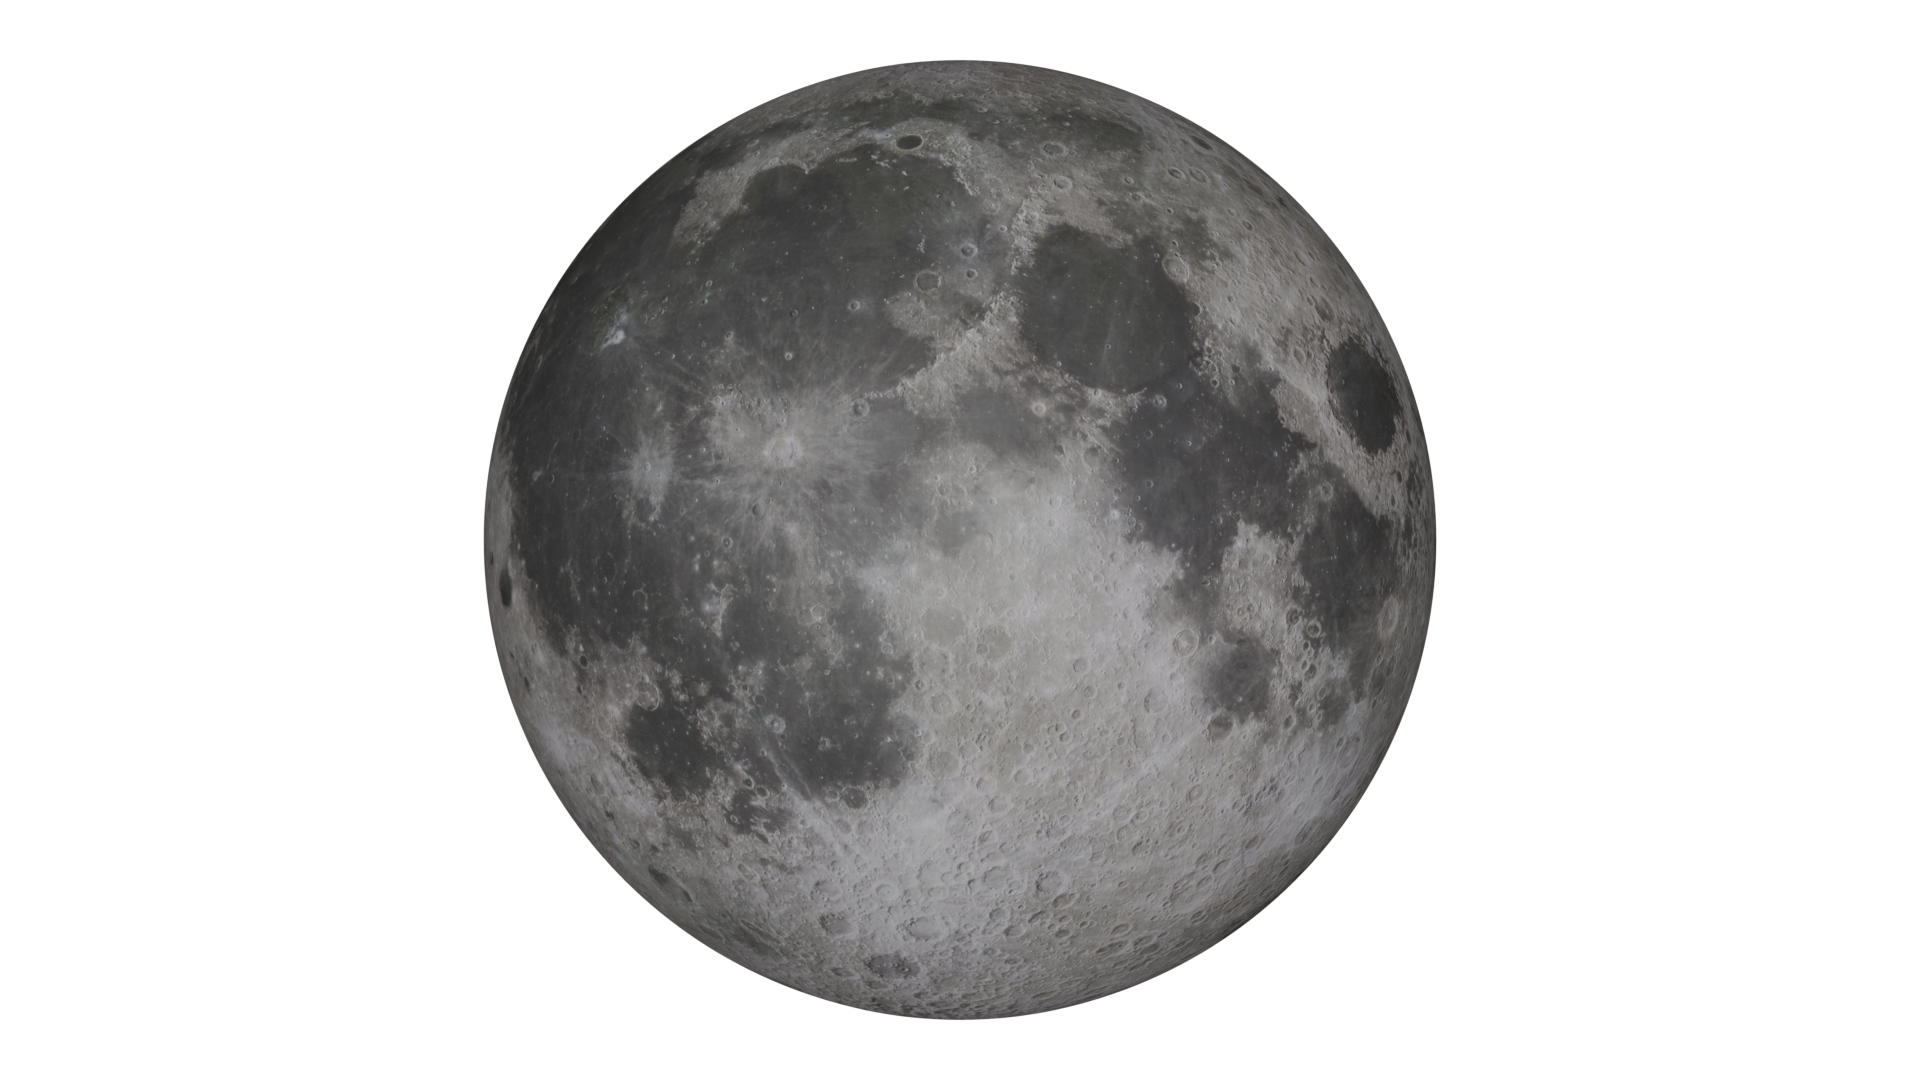
\includegraphics[width=\radpngS pt]{IMAGES/spheres/moon.png}};
% 		\end{scope}


% 		% The light gray circle (EQUATORIAL PLANE)
% 		\tdplotsetrotatedcoords{\azs}{\KtoS}{\psioffset}
% 		\begin{scope}[tdplot_rotated_coords]
		
% 		\draw[axis] (0,0,0) -- (0,-\radep,0) node [anchor=north, xshift=1pt, yshift=-5pt] {$\vec{e}_{1,\mathcal{B}}$};
% 		\draw[axis] (0,0,0) -- (\radep,0,0) node [anchor=north, xshift=18pt, yshift=6pt] {$\vec{e}_{2,\mathcal{B}}$};
% 		\draw[axis] (0,0,0) -- (0,0,\radep) node [anchor=east, xshift=26pt, yshift=3pt] {$\vec{e}_{3,\mathcal{B}}$};
	
% 		\end{scope}


% 		% ---- PRECESSION CIRCLES ----

		
% 		% syntax:  {}{}{start angle}{end angle} 
% 		% set start angle > end angle for clockwise arrow 

% 		% PRECESSION CIRCLE of orbit normal (\vec{n}) (filled white with solid line)
% 		\tdplotdrawarc[
% 			tdplot_main_coords,
% 			white,
% 			thin,
% 			fill=white
% 		]{(OS)}{\rn}{0}{360}{}{}
		
% 		% Arrow on n-circle (clockwise)
% 		\tdplotdrawarc[
% 			tdplot_main_coords,
% 			black,
% 			thin,
% 			->
% 		]{(ON)}{\rn}{\arrangnzero}{\arrangnzero-\arrangn}{}{}


% 		% PRECESSION CIRCLE of spin axis \vec{\omega} (filled white with solid line)
% 		\tdplotdrawarc[
% 			tdplot_main_coords,
% 			white,
% 			thin,
% 			fill=white
% 		]{(OS)}{\rs}{0}{360}{}{}
		
% 		% Arrow on s-circle (clockwise)
% 		\tdplotdrawarc[
% 			tdplot_main_coords,
% 			black,
% 			thin,
% 			->
% 		]{(OS)}{\rs}{\arrangszero}{\arrangszero-\arrangs}{anchor=south west, xshift=43pt, yshift=-37pt}{$\dot{\varphi}^\prime$}

% 		% Dashed circle
% 		% Circle around tip of \vec{\omega} (filled white with solid line)
% 		\tdplotdrawarc[
% 			tdplot_main_coords,
% 			black,
% 			loosely dashed,
% 		]{(ON)}{\rn}{0}{360}{}{}


		

% 		% ---- VECTORS ----
% 		% Reference axis \vec{p} (aligned with z)
% 		\draw[->, -latex', black, thin] (O) -- (K)
% 			node[above, xshift=0pt, yshift=2pt] {${\vec{p}}$};

% 		% Orbit normal \vec{n}
% 		\draw[->, -latex', black, thin] (O) -- (N)
% 			node[above, xshift=-2pt, yshift=0pt] {${\vec{n}}$};

% 		% Spin axis \vec{\omega}
% 		\draw[->, -latex', black, thin] (O) -- (S)
% 			node[right, xshift=-0.0pt, yshift=-3.0pt] {${\vec{\omega}}$};

% 		% ---- ANGLE ARCS ----
% 		% INCLINATION: Angle between k and n (\inc) - label changed to \theta
% 		\tdplotsetthetaplanecoords{\azn}
% 		\tdplotdrawarc[
% 			tdplot_rotated_coords,
% 			black,
% 			thin,
% 			->,
% 		]{(O)}{0.6}{0}{\inc}{anchor=south west, xshift=-5pt, yshift=1pt}{$i$} % syntax: {}{height?}{}{}{label}


% 		\tdplotdrawarc[
% 			tdplot_rotated_coords,
% 			black,
% 			thin,
% 			->,
% 		]{(O)}{0.50}{0}{\inc-\eps}{anchor=south west, xshift=-5pt, yshift=-1pt}{${\theta^\prime}$} 

% 		% OBLIQUITY: Angle between n and s (\eps)
% 		\tdplotsetrotatedcoords{\azn}{\inc}{0}
% 		\tdplotsetrotatedthetaplanecoords{\azs-\azn }
% 		\tdplotdrawarc[
% 			tdplot_rotated_coords,
% 			black,
% 			thin,
% 			->,
% 		]{(O)}{0.25}{0}{\eps}{anchor=south west, xshift=-10pt, yshift=0pt}{$\epsilon$}
		
% 	% ---- SPIN ROTATION MARKER ----
% 	% Create a small circle perpendicular to s 
% 	% 2. Set up rotated coordinate system aligned with s vector
% 	\tdplotsetrotatedcoords{\azs}{\KtoS}{0}
% 	% 3. Draw the circle in rotated coordinates (XY plane will be perpendicular to s)
% 	\tdplotdrawarc[
% 			tdplot_rotated_coords,
% 			shift={(0,0,0.71*\L)},
% 			black,
% 			thin,
% 			->
% 		]{(0,0,0)}{0.06}{0}{350}{anchor=west, xshift=10pt, yshift=-9pt}{$\dot{\psi}^\prime$}
% 		%{}{}{ang start}{ang end}{position}{label}


% 		% The white circle (Laplace PLANE) part 2: DASHED
% 		\tdplotsetrotatedcoords{\prec}{0}{0}
% 		\begin{scope}[tdplot_rotated_coords]
% 		\draw[loosely dashed] 
% 			plot [domain=0:360, samples=100] ({\radep * cos(\x)}, {\radep * sin(\x)});
% 		\draw[dashaxis] (0,0,0) -- (\radep,0,0) node [anchor=west, xshift=-28pt, yshift=0pt] {$\vec{e}_{1,\mathcal{P}}$};
% 		\draw[dashaxis] (0,0,0) -- (0,\radep,0) node [anchor=north, xshift=22pt, yshift=-2pt] {$\vec{e}_{2,\mathcal{P}}$};
% 		\draw[dashaxis] (0,0,0) -- (0,0,\radep) node [anchor=north, xshift=-8pt, yshift=17pt] {$\vec{e}_{3,\mathcal{P}}$};

% 		% \tdplotdrawarc[tdplot_rotated_coords,
% 		% 	black,
% 		% 	thin,
% 		% 	->,
% 		% ]{(O)}{0.2}{0}{(\azs+90-\prec)}{anchor=north, xshift=-5pt, yshift=1pt}{${\varphi^\prime}$} 
% 		% syntax: {}{height?}{}{}{label}

% 		\end{scope}
	

		
% 	\end{tikzpicture}


% 		\caption{Cassini state II}
% 		\label{fig:tikz_cassiniII}
% 	\end{subfigure}

	
% 	\caption{Schematic representation of the relative configuration of the Laplace plane normal $\vec{p}$, orbit normal $\vec{n}$, and spin axis $\vec{\omega}$ in Cassini states I and II. The obliquity $\epsilon$ is the angle between $\vec{n}$ and $\vec{\omega}$. The  circles represent the precession paths. The inclination $i$ is the angle between $\vec{n}$ and $\vec{p}$.
% 	The angles are exaggerated for visualization purposes.} %WIP
% 	\label{fig:tikz_cassini}
% \end{figure}
% %_____________________________________________________________

\subsection{Reference state}
We choose as our time origin the J2000.0 epoch and set ${t_0 = 0}$.
%
After integrating numerically Eq.~(\ref{eq_geodesic_potential}), 
% using ode45/ode89
we perform the least square fit of the solution in terms of the Euler angles and their rates of the form Eq.~\eqref{eq:generic_fit},
where the corresponding frequencies $\nu_j$ will in general include both the forced frequencies and the free inertial frequencies
$\nu_{\mathrm{f},\varphi^\prime}$, $\nu_{\mathrm{f},\theta^\prime}$, $\nu_{\mathrm{f},\psi^\prime}$, $\nu_{\mathrm{f},\mathrm{w}_{+}}$, and $\nu_{\mathrm{f},\mathrm{w}_{-}}$.

% Then, from the fit Eq.~(\ref{eq:generic_fit}) we remove the components corresponding to the free angular frequencies $\nu_{\mathrm{f},{\psi^\prime}}$  and $\nu_{\mathrm{f},{\varphi^\prime}}$. 
% %


%
% as the sum of a quadratic polynomial and a periodic part as 
% \begin{equation} \label{eq:truncated_series}
% 	%s(t) = 
% 	q^{\alpha} = 
% 	a_0 + a_1 t + a_2 t^2 + 
% 	\xi^\alpha,
% 	%\displaystyle\sum_{j = 1}^{k} s_j \sin\left(\nu_{j} t + \phi_j\right),
% 	\quad \alpha = 1,2,3,
% 	%\quad s = \varphi, \theta, \psi, \dot{\varphi}, \dot{\theta}, \dot{\psi}
% \end{equation}
% The periodic parts of the Euler angles is decomposed as
% \begin{align}
% 	\xi^{\alpha} &= \displaystyle\sum_{j = 1}^{k} s_j \sin\left(\nu_{j} t + \phi_j\right), \quad \alpha = 1,2,3,
% 	%\\
% 	% \gamma_{\theta} &= \displaystyle\sum_{j = 1}^{k} \gamma_j \sin\left(\nu_{j} t + \phi_j\right), \\
% 	% \gamma_{\psi} &= \displaystyle\sum_{j = 1}^{k} \gamma_j \sin\left(\nu_{j} t + \phi_j\right), 
% \end{align}
% where $s_j$, $\nu_{j}$, and $\phi_j$ are the amplitudes, angular frequencies and phases, respectively.



%_____________________________________________________________
% FIGURE: SPECTRA OF EULER ANGLES
\begin{figure*}
\centering

\begin{subfigure}[t]{0.495\textwidth}
	\centering
	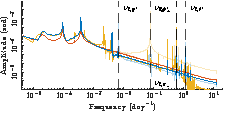
\includegraphics[
	trim=0 0 0 0, clip,
	width=\textwidth]{IMAGES/io_gamma_tile.pdf}
	\caption{Io}
	\label{fig:io_eulerI}
\end{subfigure}
%
\begin{subfigure}[t]{0.495\textwidth}
	\centering
	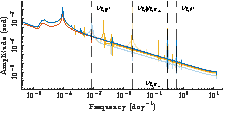
\includegraphics[
	trim=0 0 0 0, clip,
	width=\textwidth]{IMAGES/europa_gamma_tile.pdf}
	\caption{Europa}
	\label{fig:europa_eulerI}
\end{subfigure}

\vspace{.5em} % vertical space

\begin{subfigure}[t]{0.495\textwidth}
	\centering
	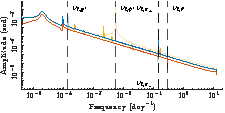
\includegraphics[
	trim=0 0 0 0, clip,
	width=\textwidth]{IMAGES/ganymede_gamma_tile.pdf}
	\caption{Ganymede}
	\label{fig:ganymede_eulerI}
\end{subfigure}
%
\begin{subfigure}[t]{0.495\textwidth}
	\centering
	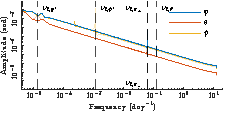
\includegraphics[
	trim=0 0 0 0, clip,
	width=\textwidth]{IMAGES/callisto_gamma_tile.pdf}
	\caption{Callisto}
	\label{fig:callisto_eulerI}
\end{subfigure}

\caption{Frequency spectrum of the periodic part of the Euler angles $(\varphi, \theta, \psi)$. 
In a faint color we show also the spectrum of the solution obtained from the IAU initial conditions, which show very high peaks at the free frequencies shown as dashed lines.}
%The green line corresponds to the least square fit of the libration amplitudes $\gamma_{\psi}$ shown in the corresponding Table.~\ref{tab:lsfit_callisto}. Discrepancies indicate the frequency fitting code needs some improvement!
\label{fig:galilean_eulerI}


\end{figure*}

% %_____________________________________________________________
% \subsection{Differential corrections}\label{se:DC_casotto}
% %_____________________________________________________________

% In order to determine the initial conditions that result in no free librations and precession % nutation
% we employ a differential correction technique. The following derivation closely follows \citet{casotto_lncm}.
% Consider the state vector of the rotating rigid body given by the Euler angles and their rates, that is,
% \begin{equation}
% \vec{x} =
% %\left( \vec{\varphi}, \dot{\vec{\varphi}}\right)^\top =
% (\varphi,\theta,\psi,\dot{\varphi},\dot{\theta},\dot{\psi} )^\top 
% = (q^1,q^2,q^3,\dot{q}^1,\dot{q}^2,\dot{q}^3 )^\top.
% \end{equation} 
% %
% %and let ${\vec{P} = \left( {A}, {B}, {C}\right)}$, be the constant parameter vector composed of the  (undistorted) moments of inertia, 
% %Consider also the function 
% %$ \vec{f}(\vec{x}, t ) $, then
% We recast Eq.~(\ref{eq:geodesic_explicit}) into a set of six first order ODEs, as
% %For compactness, we will write as usual $(\varphi,\theta,\psi)=(q^1,q^2,q^3)$.
% %
% \begin{equation}\label{eq:eom}
% 	\dot{\vec{x} } =
% 	%  \frac{d}{dt} 
% 	% \begin{pmatrix}
% 	% 	\vec{\varphi}\\
% 	% 	\dot{\vec{\varphi}}
% 	% \end{pmatrix} =
% 	\vec{f}(\vec{x}, t ),
% 	\quad \vec{x}(t_0) = \vec{x}_0,
% \end{equation}
% % where $  \vec{f}(\vec{x}, t ) = (F_1, F_2, \dots, F_{6})$ with
% where 
% \begin{align}
% 	\vec{f} &= 
% 	\begin{pmatrix}
% 	\dot{q}^1 \\ \dot{q}^2 \\ \dot{q}^3 \\
% 	-{\Gamma}^{1}_{\beta\gamma} \dot{q}^\beta \dot{q}^\gamma 
% 	+{g}^{1\beta} \frac{\partial \mathcal{U}}{\partial q^\beta}
% 	\\%
% 	-{\Gamma}^{2}_{\beta\gamma} \dot{q}^\beta \dot{q}^\gamma 
% 	+{g}^{2\beta} \frac{\partial \mathcal{U}}{\partial q^\beta}
% 	\\% 
% 	-{\Gamma}^{3}_{\beta\gamma} \dot{q}^\beta \dot{q}^\gamma 
% 	+{g}^{3\beta} \frac{\partial \mathcal{U}}{\partial q^\beta}
% 	\end{pmatrix}.
% 	% -{\Gamma}^{\alpha}_{\beta\gamma} \dot{q}^\beta \dot{q}^\gamma 
% 	% +{g}^{\alpha\beta} \frac{\partial \mathcal{U}}{\partial q^\beta}, & \alpha = 1,2,3,
% \end{align}
% %
% %Suppose that  we have available the full dynamical state of our body from an ephemeris, and we treat this ephemeris data as observations (measurements), i.e., $\vec{y}_i = \vec{y}(t_i)$ of the rigid body at different discrete time $t_i, \; i = 1, \dots l$. 
% % In general the observations can be related to the state vector components via a generic model function $\vec{G}(\vec{x}, t )$.
% % In our case however the synthetic observations, which we denote by  $\vec{y}(t)$, are a time series of the state vector components and the model function is just the identity, that is ${\vec{G}(\vec{x},t) = \vec{x}(t)}$. 
% %Nonetheless, we will keep writing $\vec{G}$ for clarity.
% %Thus we can write
% % depending on the state vector and the vector $\vec{Q}$ of constant, non-dynamical parameters. 
% %and there are no parameter $\vec Q$, and  it is

% Consider also the synthetic observations, which we can write as the sum of the true state and a vector of errors $\vec{\varepsilon}(t)$, that is,
% \begin{equation}\label{eq:y_x_plus_eps}
% 	\vec{y}(t) = 
% 	\vec{x}(t;\vec{x}_0) + \vec{\varepsilon}(t).
% \end{equation}
% In practice,  the synthetic observations corresponding to the Cassini state $\vec{y}(t)$, are obtained by first integrating to rotational equations from the initial guess at the current iteration, which we denote by ${\vec{x}_0^* = \vec{x}_0^{(n-1)}}$, and then subtracting from ${\vec{x}(t;\vec{x}_0^*)}$ the periodic terms corresponding to the free frequency components obtained from the least square fit. This can be written
% %
% \begin{equation}\label{eq:synth_obs}
% 	\vec{y}(t) = 
% 	\vec{x}(t;\vec{x}_0^*) -
% 	\begin{bmatrix}
% 		\sum_j s_{\mathrm{f},j}^{1} \sin\left(\nu_{\mathrm{f},j}^{} t + \phi_{\mathrm{f},j}^{1}\right)
% 		\\
% 		\sum_j s_{\mathrm{f},j}^{2} \sin\left(\nu_{\mathrm{f},j}^{} t + \phi_{\mathrm{f},j}^{2}\right)
% 		\\
% 		\vdots
% 		\\
% 		\sum_j \nu_{\mathrm{f},j}^{} s_{\mathrm{f},j}^{3} \cos\left(\nu_{\mathrm{f},j}^{} t + \phi_{\mathrm{f},j}^{3} \right)
% 	\end{bmatrix},
% 	% \begin{pmatrix}
% 	%   \gamma_{\mathrm{f},\psi}\sin\left(\nu_{\psi}t + \phi_{\psi}\right) 
% 	%   \gamma_{\mathrm{f},\psi}\sin\left(\nu_{\psi}t + \phi_{\psi}\right)
% 	%  \\
% 	%   \nu_{\psi}\gamma_{\mathrm{f},\psi}\cos\left(\nu_{\psi}t + \phi_{\psi}\right) 
% 	%   \nu_{\psi}\gamma_{\mathrm{f},\psi}\cos\left(\nu_{\psi}t + \phi_{\psi}\right)
% 	% \end{pmatrix}.
% \end{equation}
% where a superscript ${\alpha = 1,2,3}$ denotes a term corresponding to the state variable $q^\alpha$, and the periodic components of $\dot{q}^\alpha$ have been written simply differentiating Eq.~\eqref{eq:generic_fit} with respect to time.
% % \begin{equation}\label{eq:synth_obs}
% % 	\vec{y}(t) = 
% % 	% \vec{G}(\vec{x}, t ) 
% % 	\vec{x}(t) 
% % 	+ \vec{\varepsilon}(t), %cov??
% % \end{equation}
% % %
% % where $\vec{\varepsilon}(t)$ is the vector of residuals (?? probably this should be removed).
% % %
% %Note that we require $p<n$ at any time epoch, that is fewer observations than there are state vector components. 
% %
% % We use a nonlinear least squares inversion to solve for the unknown parameters. 
% % Our observations are the radial are constituted by the  numerically integrated rotational equations starting from an initial guess. 
% %
% Now we describe the iterative differential correction scheme needed to determine the initial conditions ${\vec{x}_0 = \vec{x}_0^{(n)}}$, that minimize the residuals ${\vec{y}(t) - \vec{x}(t; \vec{x}_0)}$.
% %(maybe opposite sign)
% % \begin{align} \label{eq:dy_y_minus_xatx0}
% % 	%\delta \vec{y}_i &= \vec{G}(\vec{x},t_i) - \vec{y}_i,
% % 	% \delta \vec{y}(t) &= \vec{y}(t) - \vec{x}(t; \vec{x}_0^*), %!!! check this  
% % 	\delta \vec{y}(t) &= \vec{y}(t) - \vec{x}(t; \vec{x}_0),
% % \end{align}
% %parameter vectors $\vec{P}$ and $\vec{Q}$ 
% %to the synthetic observation. 
% % Call 
% % $\vec{x}^* = \vec{x}(t;\vec{x}_0)$. (Does this make sense?)
% If a reasonable initial guess $ \vec{x}_0^*$ is available, and the evolution  of the Euler angles and their rates corresponding to the true Cassini state ${\vec{x} = \vec{x}(t;\vec{x}_0)}$ % and if $\vec{x}$, the true trajectory, and 
% remains sufficiently close to the reference trajectory
% ${\vec{x}^* = \vec{x}(t;\vec{x}_0^*)}$
% then the Cassini state trajectory can be expanded in a Taylor's series about the reference trajectory obtained from the initial guess (from IAU model) at each point in time. If this expansion is truncated to eliminate higher order terms, then the deviation in the state from the reference trajectory can be described by a set of linear differential equations with time dependent coefficients. A linear relation between the observation deviation and the state deviation can be obtained by a similar expansion procedure. Then, the nonlinear problem in which the complete state vector is to be estimated can be replaced by a linear orbit determination problem in which the deviation from some reference solution is to be determined \citep{casotto_lncm}.
% %We assume that a reference solution $\vec{x}^* (t, \vec{x}_0 , \vec{P}^* )$ of the dynamical equations is known in terms of a set of reference values $\vec{P}^*$ for the system parameters.
% %The measurement model is likewise assumed to be known in terms of a set of reference values of the parameters $\vec{Q}^*$. 
% % Synthetic Cassini state $\vec{y}$ computed from Eq.~(\ref{eq:synth_obs}),
% We will see how we can use a discrete set of synthetic observations ${\vec{y}_i = \vec{y}(t_i)}$, %where $i = 1, ..., l$, is a set to obtain the corrected values for the initial state $\vec{x}_0$.
% to obtain the correct initial conditions that result in zero-amplitude free motion, that is the Cassini state.
% % and the parameters $\vec{P}^*$. % and $\vec{Q}^*$.
% %
% If we introduce the variations ${\delta \vec{x}}$ of the state vector and the observations we can write
% \begin{align}
% 	\label{eq:dx_x_xstar}
% 	\delta \vec{x}(t)
% 	&= \vec{x}(t;\vec{x}_0)
% 		- \vec{x}(t;\vec{x}_0^*),
% 	% = \vec{x} - \vec{x}^*,
% % \vec{x}(t) &= \vec{x}^*(t) + \delta \vec{x}, \\
% 	\\ 
% 	\label{dy_y_xstar}
% 	\delta \vec{y}(t)
% 	&= \vec{y}(t) - \vec{x}(t;\vec{x}_0^*).
% % \vec{y}(t) &= \vec{G}(\vec{x}^*, t) + \delta \vec{y},
% % \\
% %\vec{P} &= \vec{P}^* + \delta \vec{P}, %\\
% %
% %\vec{Q} &= \vec{Q}^* + \delta \vec{Q}.
% \end{align}
% A first-order expansion of the forcing yields
% \begin{align}
% 	\label{eq:f_fstar_dfdx}
% 	\vec{f}(\vec{x}, t ) =  \vec{f}(\vec{x}^*, t )
% 	+ \pdv{ \vec{f}}{ \vec{x}} \bigg|_{\vec{x}^*}
% 	\delta \vec{x}(t).
% 	% + \vec{\Lambda}(t)
% 	%+\pdv{ \vec{f}}{ \vec{P}} \bigg|^* \delta \vec{P}(t),
% 	%  \\
% 	% \vec{G}(\vec{x}, t ) &=  \vec{G}(\vec{x}^*, t ) % \vec{Q}^*
% 	% + \pdv{ \vec{G}}{ \vec{x}} \bigg|^* \delta \vec{x}(t).
% 	% %+\pdv{ \vec{G}}{ \vec{Q}} \bigg|^* \delta \vec{Q}(t_i).
% \end{align}
% %
% Differentiating Eq.~\eqref{eq:dx_x_xstar}  with respect to time and substituting  Eqs.~\eqref{eq:eom}  and \eqref{eq:f_fstar_dfdx}, we obtain the equations of the differential dynamics, which can be written as
% %
% \begin{align}\label{vareq_ext}
% 	\delta\dot{\vec{x}}(t) &= \vec{\Lambda}(t) \delta\vec{x}(t),
% 	% + \vec{B}(t) \vec{p},
% \end{align}
% %
% where we defined
% \begin{equation}
% % \vec{\Lambda}(t) = \pdv{\vec{f}}{\vec{x}}\left(\vec{x},t; \vec{x}_0\right),
% \vec{\Lambda}(t) = \pdv{\vec{f}}{\vec{x}}\bigg|_{\vec{x^*}}. %\quad 
% %\vec{B}(t) = \pdv{\vec{f}}{\vec{P}}\bigg|^*, \quad 
% %\tilde{\vec{H}}_i = \pdv{\vec{G}}{\vec{x}}\bigg|^*_i.
% %\quad 
% %\vec{K}_i = \pdv{\vec{G}}{\vec{Q}}\bigg|^*_i.
% \end{equation}
% %
% Using Eqs.~\eqref{eq:y_x_plus_eps} and \eqref{dy_y_xstar}, we can also express the differential observations as
% \begin{equation}
% 	\delta\vec{y}(t) = 
% 	\delta\vec{x}(t) 
% 	+ \vec{\varepsilon}(t).
% \end{equation}

% % \begin{align}\label{ve_1}
% % 	\delta\dot{\vec{x}}(t) &= \pdv{\vec{f}}{\vec{x}}\bigg|^* \delta \vec{x}(t),
% % 	% + \pdv{\vec{f}}{\vec{P}}\bigg|^* \delta \vec{P}, 
% % 	%\\
% % 	% \label{ve_2}
% % 	% \delta \vec{y}_i &= \pdv{\vec{G}}{\vec{x}} \bigg|^*\delta \vec{x}(t_i) %+ \pdv{\vec{G}}{\vec{Q}}\bigg|^* \delta \vec{Q} 
% % 	% + \vec{\varepsilon}_i.
% % \end{align}
% %Note that in equation (22.9) \( \pdv{\vec{f}}{\vec{P}} \) is the total derivative of \( \vec{f} \) with respect to the parameter vector \( \vec{P} \), since \( \vec{f} \) is a function of \( \vec{P} \) both directly and through the state \( \vec{x}(t, \vec{P}) \). It is nevertheless to be computed by considering the dynamical state \( \vec{x} \) as constant.
% %
% % If, for convenience, we write the deviations using small case letters as
% % \begin{equation}
% % \delta\vec{x} = \delta \vec{x},
% % \quad \delta\vec{y}_i = \delta \vec{y}_i,
% % % \quad \vec{p} = \delta \vec{P}, 
% % %= [\delta {A}, \delta {B}],% \delta {C}], 
% % %	\quad \vec{q} = \delta \vec{Q},
% % \end{equation}
% %then we can write %Eq.~(\ref{ve_1}) %and  (\ref{ve_2}) become


% %Note that (\ref{vareq_ext}) is the variational equation associated with (\ref{eq:eom}) extended to include the system parameters $\vec{P} = ({A}, {B})$. %, {C})$.
% %We now write the explicit expression of the matrices of partial derivatives defined above.
% %
% %\setcounter{MaxMatrixCols}{12}
% %\begin{align}
% %	\vec{\Lambda}(t) = 
% %	\begin{pmatrix}
% %		0 & \frac{({B} - {C}) \omega_3}{{A}} & \frac{({B} - {C}) \omega_2}{{A}} \\
% %		\frac{({C} - {A}) \omega_3}{{B}} & 0 & \frac{({C} - {A}) \omega_1}{{B}} \\
% %		\frac{({A} - {B}) \omega_2}{{C}} & \frac{({A} - {B}) \omega_1}{{C}}&0 
% %	\end{pmatrix}
% %\end{align}
% %
% %
% %
% %\begin{equation}
% %	\vec{B}(t) =
% %	\begin{pmatrix}
% %		-\frac{\omega_2 \omega_3 ({B} - {C})}{{A}^2} & \frac{\omega_2 \omega_3}{{A}} \\%& -\frac{\omega_2 \omega_3}{{A}} \\
% %		-\frac{\omega_3 \omega_1}{{B}} & -\frac{\omega_3 \omega_1 ({C} - {A})}{{B}^2} 	\\%& \frac{\omega_3 \omega_1}{{B}} \\
% %		\frac{\omega_1 \omega_2}{{C}} & -\frac{\omega_1 \omega_2}{{C}}\\ %& -\frac{\omega_1 \omega_2 ({A} - {B})}{{C}^2} \\
% %		%		0 & 0 & 0 \\
% %		%		0 & 0 & 0 \\
% %		%		0 & 0 & 0
% %	\end{pmatrix}
% %\end{equation}
% %
% %\begin{align}
% %	\tilde{\vec{H}}_i
% %	&= \frac{\partial \vec{G}}{\partial \vec{x}} \bigg|^*_i= \mathbb{I}_{3\times3} = 
% %	\begin{pmatrix}
% %		1&0&0\\0&1&0\\0&0&1
% %	\end{pmatrix}.
% %	%	\left[ 1, 1, 1, 1,1,1,1,1,1,1,1,1\right]_i^*
% %\end{align}


% %	\begin{align}
% 	%		\vec{K}_i & = \frac{\partial \vec{G}}{\partial \vec{Q}} \bigg|^*_i=
% 	%		\left[
% 	%		\pdv{\vec{G}}{\lambda_2}, \ldots, 
% 	%		\pdv{\vec{G}}{\lambda_5}
% 	%		\right]_i^* = 
% 	%		\begin{pmatrix}
% 		%			\frac{\partial \rho_1}{\partial \lambda_2}& \dots & \frac{\partial \rho_1}{\partial \lambda_5} \\
% 		%			\vdots &   \vdots & \vdots \\
% 		%			\frac{\partial \rho_5}{\partial \lambda_2}& \ldots  &\frac{\partial \rho_5}{\partial \lambda_5}
% 		%		\end{pmatrix}_i^*
% 	%		= \\ =&
% 	%		\begin{pmatrix}
% 		%			0&0&0&0& \\
% 		%			\frac{\partial \rho_5}{\partial \lambda_2}& 0 & 0 & 0\\
% 		%			0&  \frac{\partial \rho_5}{\partial \lambda_2}& 0 & 0  \\
% 		%			0& 0  &\frac{\partial \rho_5}{\partial \lambda_2}& 0 \\
% 		%			0& 0 & 0  &	\frac{\partial \rho_5}{\partial \lambda_2}
% 		%		\end{pmatrix}_i^*
% 	%	\end{align}
% %	


% In order to solve for the initial state and the parameters, we need to relate the deviation ${  \delta \vec{y}(t) }$ at time $ t $ to the state deviation ${ \delta\vec{x}_0  = \delta \vec{x}(t_0) }$ at epoch $ t_0 $. 
% %and the parameter deviation \( \vec{p} = \delta \vec{P} \).
% This can be done by mapping the linear state deviation using the differential relationship
% \begin{equation}
% \delta \vec{x} = \pdv{\vec{x}}{\vec{x}_0} \delta \vec{x}_0.%+ \pdv{\vec{x}}{\vec{P}} \delta \vec{P}.
% \end{equation}
% %
% We call the matrix of partial derivative of the flow with respect to the initial state ${\vec{\Phi}(t, t_0) = \partial\vec{x}/\partial\vec{x}_0}$ the dynamical state transition matrix (STM).
% %, and $\vec{\Phi}_{\vec{xp}}(t, t_0) = \partial\vec{x} /\partial \vec{P}$ the parameter state transition matrix.
% Then the solution to Eq.~(\ref{vareq_ext}) can be written in terms of the state transition matrix as
% \begin{equation}
% 	\delta\vec{x}(t) = 
% 	\vec{\Phi}(t, t_0) \delta\vec{x}_0. 
% 	%+\vec{\Phi}_{\vec{xp}}(t, t_0) \vec{p}.
% \end{equation}
% %
% Furthermore, we can write the residual in terms of the initial state deviation $\delta\vec{x}_0$ % and the parameter deviations $\vec{p}$ 
% \begin{equation}\label{eq:22.23}
% 	\delta\vec{y}(t) = 
% 	%\tilde{\vec{H}}_i	
% 	\vec{\Phi}(t, t_0) \delta\vec{x}_0 
% 	%+\tilde{\vec{H}}_i	\vec{\Phi}_{\vec{xp}}(t, t_0) \vec{p} 
% 	%+ \vec{K}_i \vec{q} 
% 	+ \vec{\varepsilon}(t),
% 	% \quad i = 1, \dots, l.
% \end{equation}
% %That is
% %\begin{equation}\label{eq:22.23}
% %	\delta\vec{y}_i = 
% %	\vec{\Phi}(t, t_0) \delta\vec{x}_0 + 
% %	\vec{\Phi}_{\vec{xp}}(t, t_0) \vec{p} 
% %	+ \vec{K}_i \vec{q} 
% %	+ \vec{\varepsilon}_i, \quad i = 1, \dots, l.
% %\end{equation}
% %
% % Equation~(\ref{eq:22.23}) can be written more compactly in matrix form if we define two new matrices:
% % \begin{align}
% % 	\vec{H}_{i}^{\delta\vec{x}} &= \tilde{\vec{H}}_i \vec{\Phi}(t, t_0). 
% % 	%\\
% % 	%\vec{H}_{i}^{\vec{p}}  &= \tilde{\vec{H}}_i \vec{\Phi}_{\vec{xp}}(t, t_0). % + \vec{K}_{i}^{\vec{q}} .
% % \end{align}
% %
% % Then we can also write:
% % \begin{equation}
% % 	\delta\vec{y}_i = 
% % 	\vec{H}_{i}^{\delta\vec{x}} \delta\vec{x}_0
% % 	% \begin{pmatrix}
% % 	% 	\vec{H}_{i}^{\delta\vec{x}} 	\vec{H}_{i}^{\vec{p}} %& \vec{K}_i^{\vec{q}} 
% % 	% \end{pmatrix}
% % 	% \begin{pmatrix}
% % 	% 	\delta\vec{x}_0 \\ \vec{p} %\\ \vec{q} 
% % 	% \end{pmatrix}
% % 	+ \vec{\varepsilon}_i, \quad  i = 1, \ldots, l .
% % \end{equation}
% %

% %
% %In practice the estimate with the full vector of moments and products of inertia will converge only under special circumstances.
% %For instance, it is clear  that Eq.~(\ref{eq:euler_solid_moon_williams})  in absence of torques, i.e., $\vec{K} = 0$, is  invariant under a transformation of the type 
% %, but that remains true even when $\vec{K}$ originates from the interaction of the  and it can be shown that this is true also when the degree-2 pote
% % \begin{equation}%\label{eq:invariance_I}
% % 	\vec{I}_s \mapsto k \vec{I}_s, \quad k \neq 0.
% % \end{equation}
% % Which leaves no hopes of estimating the full inertia tensor in absence of torques.
% % If $\vec{K}$ (or $\mathcal{U}$) is known i.e., it does not depend on the outer shell moments of inertia but only on the whole body-gravity field coefficients, then at least in principle the full shell tensor of inertia  can be estimated, this is in a way analogue to combining the degree-2 gravity fields and relative moments difference \citep[see e.g.,][]{2014JGRE..119.1546W}.
% %
% % \subsection{Multi-arc method}
% % Mismodeling within the rotational equations is inevitable, given the dependence on the (unknown) interior structure of Ganymede. Effects that are not properly considered in the dynamical model will  produce errors that accumulate with time. For these reasons, a single-arc estimation of the solution vector may be inadequate.
% % In the multi-arc method, the state vector $\vec{x}$ at the  beginning of each arc (i.e., initial conditions )  are characteristic of the specific arc and therefore are called local parameters. The other free parameters describing the force model, in our case the moments of inertia $\vec{P}$ are shared by all arcs, and are called global parameters.
% % These effects can be absorbed using a multi-arc filter that provides sufficient over-parameterization of the problem. This method includes an independent estimation of the local parameter vector $l_i$, i.e., initial conditions  relative to each single arc $i$ and a combined estimation of the global parameter vector $\vec{P}$, shared by all arcs. The tracking phase is divided into $n$ arcs: the duration of the single arc must be neither too long, in order to avoid accumulation of dynamical errors, nor too short, for in this case the solution could be driven to instability. 
% %
% %%See Parisi & Iess conference paper 

% %\subsection{Computing the state transition matrix}

% The computation of the state transition matrix can be carried out by noting that by taking the gradient of both sides of Eq.~\eqref{eq:eom} with respect to the state at epoch, we find
% \begin{equation}
% 	\frac{\partial \dot{\vec{x}}(t)}{\partial \vec{x}_0} = \frac{\partial \vec{f}}{\partial \vec{x}} \Bigg|_{\vec{x}^*} \frac{\partial \vec{x}(t)}{\partial \vec{x}_0}. %\label{eq:22.28}
% \end{equation}
% The same equation can be written in the form
% \begin{equation} \label{eq:eom_STM}
% 	\dot{\vec{\Phi}}(t, t_0) = \vec{\Lambda}(t) \vec{\Phi}(t, t_0), \quad \vec{\Phi}(t_0, t_0) = \vec{1}_{6\times6}. % \label{eq:22.32}
% \end{equation}
% Clearly, the differential equations for the STMs, Eq.~\eqref{eq:eom_STM}, are coupled with the system's equations of motion, Eq.~(\ref{eq:geodesic_explicit}), and thus need to need be numerically integrated simultaneously.

% %
% % Taking the gradient of both sides of Eq.~\eqref{eq:eom}  with respect to the dynamical parameters \( \vec{P} \), we obtain
% % \begin{equation}
% % 	\frac{\partial \dot{\vec{x}}(t)}{\partial \vec{P}} = \frac{\partial \vec{f}}{\partial \vec{x}} \Bigg|^* \frac{\partial \vec{x}(t)}{\partial \vec{P}} + \frac{\partial \vec{f}}{\partial \vec{P}} \Bigg|^* . \label{eq:22.33}
% % \end{equation}
% % The same equation can be written in the form
% % \begin{align}
% % 	\dot{\vec{\Phi}}_{\vec{xp}}(t, t_0) = \vec{\Lambda}(t) \vec{\Phi}_{\vec{xp}}(t, t_0) + \vec{B}(t), \quad {\vec{\Phi}}_{\vec{xp}}(t_0, t_0) = \vec{0}_{6\times 1} 
% % \end{align}

% \subsection{Batch processor algorithm}

% The batch processor  algorithm proceeds through multiple iterations to refine the initial conditions $\vec{x}_0$ in order to minimize the residuals between the state $\vec{x}(t;\vec{x}_0)$ and the synthetic Cassini state $\vec{y}(t)$ computed as in Eq.~\eqref{eq:synth_obs}.
% %
% To do that, we need to estimate the state deviation vector $\tilde{\delta\vec{x}}_0$ at a reference time, $t_0$.
% Each iteration consists of:
% %
% \begin{enumerate}
% 	\item Initializing ${ {\vec{A}} = \vec{0}_{6\times6} }$ and ${ \vec{b} = \vec{0}_{6\times1}  }$, where ${ {\vec{A}} }$ is the information matrix and $ \vec{b} $ is the normal matrix.
% 	\item Iterating through the unique measurement times $t_i$, solving the differential equations to propagate the state and state transition matrix \( \vec{\Phi} \) to each of those times.
% 	\item For each unique time, accumulating the contributions to $ {\vec{A}} $ and $ \vec{b} $ based on the residual between observed and computed measurements.
% 	\item Solving the normal equations to find the least squares solution and update the state estimate.
% \end{enumerate}
% %
% The normal equations that we need to solve to obtain the deviation vector $ \delta\vec{x}_0$, %$ \tilde{\delta\vec{x}}_0$, 
% are given by:
% %
% \begin{equation}
% 	% {\vec{A}}  \tilde{\delta\vec{x}}_0 = \vec{b},
% 	{\vec{A}}  \delta\vec{x}_0 = \vec{b},
% \end{equation}
% %
% where the matrices $ {\vec{A}} $ and $ \vec{b} $  are computed using:
% \begin{equation}
% 	{\vec{A}} = %	\vec{P}_0^{-1} + 
% 	\displaystyle\sum_{i = 1}^{l} \vec{\Phi}(t_i,t_0)^\top  %\vec{W}_i 
% 	\vec{\Phi}(t_i,t_0),  \quad
% 	\vec{b} = 	
% 	%\vec{P}_0^{-1}\vec{\hat{x}}_0 + 
% 	\displaystyle\sum_{i = 1}^{l} \vec{\Phi}(t_i,t_0)^\top   %\vec{W}_i
% 	\delta\vec{y}_i,
% \end{equation}
% having defined ${\delta \vec{y}_i = \vec{y}(t_i) - \vec{x}(t_i,\vec{x}_0^*)}$.
% % \begin{equation}
% % 	\delta \vec{y}_i =
% % 	% \delta \vec{y}(t_i) =
% % 	\vec{y}(t_i) - \vec{x}(t_i,\vec{x}_0^*).
% % \end{equation}
% % \begin{equation}
% % 	{\vec{A}} = %	\vec{P}_0^{-1} + 
% % 	\displaystyle\sum_{i = 1}^{l} \vec{H}_i^\top  %\vec{W}_i 
% % 	\vec{H}_i,  \quad
% % 	\vec{B} = 	
% % 	%\vec{P}_0^{-1}\vec{\hat{x}}_0 + 
% % 	\displaystyle\sum_{i = 1}^{l} \vec{H}_i^\top   %\vec{W}_i
% % 	\delta\vec{y}_i.
% % 	%=
% % 	%\vec{P}_0^{-1}\vec{\hat{x}}_0 +
% % 	%\displaystyle\sum_{i = 1}^{l} \vec{H}_i^\top  %\vec{W}_i 
% % 	%(\vec{y}_i - 	\vec{x}(t_i) ),
% % 	% ( \vec{y}_i -  \vec{G}(	\vec{x},  \vec{Q}, t_i)).
% % \end{equation}
% %where $\vec{W}_i $ is the observation weight matrix, and $\vec{P}_0$ is the error covariance matrix associated to the a priori estimate $\vec{\hat{x}}_0$.
% %
% % For simplicity, we can assume $\vec{W}_i  = \mathbb{I}_{12\times 12}$, $\vec{\hat{x}}_0 = 0_{12\times1}$, and the diagonal elements of $	\vec{P}_0$ should be taken as very small depending on the accuracy of the initial guess, for instance since the position and velocities in the present case are taken directly from the ephemerides we can set the corresponding diagonal terms to e.g., $10^{12}$ in this way they will be kept fixed during the estimation process, correctly tuning $	\vec{P}_0$ proves to be quite important for the algorithm to converge.
% %
% %	\begin{equation}
% 	%		{\vec{A}} = {\vec{A}} + \vec{H}_i^\top   \vec{H}_i, \quad \vec{B} = \vec{B} +  \vec{H}_i^\top  ( \vec{y}_i -  \vec{G}(	\vec{x},  \vec{Q}, t_i)),
% %	\end{equation}
% %
% %
% %
% %where the residual vector
% %$  \delta\vec{y}_i  = \vec{y}_i -  \vec{G}(	\vec{x},  \vec{Q}, t_i) $
% %${\delta\vec{y}_i  = \vec{y}_i - 	\vec{x}(t_i)}$
% %represents the difference between the observed and computed measurements for the dynamical state at each unique time \( t_i \).
% %
% Lastly, the state vector at the  $n^{\mathrm{th}}$ iterations, that is, $ \vec{x}_0^{(n)}$, is updated as:
% %
% \begin{equation}
% 	\vec{x}_0^{(n)}= \vec{x}_0^{(n-1)} +  \delta\vec{x}_0,
% \end{equation}
% % \begin{equation}
% % 	\vec{x}_0= \vec{x}_0 +  \delta\vec{x}_0,
% % 	\quad 
% % 	\tilde{\vec{x}}_0 = 
% % 	\begin{pmatrix}
% % 		\vec{x}_0% \\
% % 		\vec{P} %\\
% % 			\vec{Q}
% % 	\end{pmatrix}.
% % \end{equation}
% that is the new state vector of initial conditions to be used in the following iteration, or the converged value.
% % Note that at each iteration we update also the synthetic observations $\vec{y}(t)$ computed from Eq.~\eqref{eq:synth_obs}.

% % NEW
% In order to compute the STM, it is required to evaluate the matrix $\vec{\Lambda}(t)$, whose components are the of partial derivatives of $\vec{f}$  with respect to the state vector  $\vec{x}$. The lengthy explicit expressions of the partial derivatives with the symbolic computation capabilities of Wolfram Mathematica, and we omit them here.


% The quantities obtained, constitute the set of synthetic observations corresponding to the Cassini state  evolution of the Euler angles obtained by integrating the rotational equation from the IAU model initial conditions we estimate the correct initial conditions 
% %$(\vec{\varphi}(t_0),\dot{\vec{\varphi}}(t_0))$
% as described in Sect.~\ref{se:DC_casotto}.

% The estimated initial conditions for the Galilean satellites at the J2000.0 epoch, in the ICRF frame are given in Table~\ref{tab:euler_initial_conditions}.

% \subsection{Root mean square}

% The best estimate of the observation error is given by


% \begin{align}
% 	\hat{\vec{\varepsilon}}_i &= \delta\vec{y}_i - \vec{H}_i\tilde{\delta\vec{x}}_0 \label{eq:22.73}
% \end{align}

% The root mean square (rms) of the observation residuals generally is computed and may be used as a measure of convergence; when the rms no longer changes, within some given tolerance, the solution is assumed to have converged. The rms is computed from
% \begin{equation}
% 	\text{rms} = \sqrt{\frac{\displaystyle\sum_{i=1}^{l} \hat{\vec{\varepsilon}}_i^\top %R^{-1}
% 			\hat{\vec{\varepsilon}}_i}{k}} \label{eq:22.74}
% \end{equation}
% where \(\hat{\vec{\varepsilon}}_i\) is a \(p\)-vector and \(k = l \times p\). Hence, \(k\) is the total number of observations. 
% %The equation \eqref{eq:22.74} is referred to as the  rms.
% % If the rms is computed without including the weighting matrix, \(R^{-1}\), it may be referred to as the unweighted rms or just the rms.

	
	
% \text{and } \vec{r}_B \text{ is the position vector with respect to the body axes, thus:}
	

\section{Results}\label{sec:num_experiments}
\textit{[Placeholder for Plots - To be generated]}
Figure X illustrates the evolution of the formal uncertainty ($1\sigma$) of the moment of inertia differences $(B-A)$ and $(C-A)$. We observe that:
\begin{itemize}
    \item The formal uncertainty decreases as $1/\sqrt{t}$, as expected.
    \item The inclusion of the full geodesic coupling allows for the decorrelation of the libration amplitude from the inertia parameters after approximately 14 days of tracking.
    \item The expected relative precision for the moments of inertia is on the order of $10^{-4}$.
\end{itemize}

\section{Conclusion}
We have presented a rigorous formulation of rotational dynamics for extended, deformable bodies using a geodesic approach on a Finsler manifold. This method allows for a consistent treatment of tidal-rotational coupling. The covariance analysis demonstrates that this formulation is numerically stable and suitable for precise parameter estimation in future planetary missions.




% Our model, however, is based on a rigid-body approximation. This is a significant simplification, as Ganymede, Europa, and possibly Callisto are thought to harbor subsurface liquid oceans, while Io may possess a magma ocean. These liquid layers, along with tidal distortions of the moments of inertia, are not accounted for in the present model but may have important effects on the dynamics.
% Additionally, the torques due to the interaction of the figure of the satellites with the figure of Jupiter are not modelled here as the McCullagh's potential does not include them, but may be important \citep[see, e.g.,][]{1981M&P....25....3E, 2021AJ....161..105P}.
% Moreover, the translational and rotational equations should, ideally, be integrated simultaneously, since they are coupled in their most general formulation.

% Future work should therefore focus on extending the current framework to incorporate different plausible interior structure models to properly evaluate the effects of coupling mechanisms between the  solid and liquid layers. 

% Nevertheless, the results presented here provide an accurate rigid-body reference model that can be used to interpret future high-precision measurements from missions like Juice and Europa Clipper.




\backmatter

\bmhead{Supplementary information}

Not applicable

% If your article has accompanying supplementary file/s please state so here. 

% Authors reporting data from electrophoretic gels and blots should supply the full unprocessed scans for key as part of their Supplementary information. This may be requested by the editorial team/s if it is missing.

% Please refer to Journal-level guidance for any specific requirements.

\bmhead{Acknowledgements}

% Acknowledgements are not compulsory. Where included they should be brief. Grant or contribution numbers may be acknowledged.

% Please refer to Journal-level guidance for any specific requirements.

\section*{Declarations}

Not applicable

% Some journals require declarations to be submitted in a standardised format. Please check the Instructions for Authors of the journal to which you are submitting to see if you need to complete this section. If yes, your manuscript must contain the following sections under the heading `Declarations':

% \begin{itemize}
% \item Funding
% \item Conflict of interest/Competing interests (check journal-specific guidelines for which heading to use)
% \item Ethics approval and consent to participate
% \item Consent for publication
% \item Data availability 
% \item Materials availability
% \item Code availability 
% \item Author contribution
% \end{itemize}

% \noindent
% If any of the sections are not relevant to your manuscript, please include the heading and write `Not applicable' for that section. 

%%===================================================%%
%% For presentation purpose, we have included        %%
%% \bigskip command. Please ignore this.             %%
%%===================================================%%
\bigskip
\begin{flushleft}%
Editorial Policies for:

\bigskip\noindent
Springer journals and proceedings: \url{https://www.springer.com/gp/editorial-policies}

\bigskip\noindent
Nature Portfolio journals: \url{https://www.nature.com/nature-research/editorial-policies}

\bigskip\noindent
\textit{Scientific Reports}: \url{https://www.nature.com/srep/journal-policies/editorial-policies}

\bigskip\noindent
BMC journals: \url{https://www.biomedcentral.com/getpublished/editorial-policies}
\end{flushleft}

\begin{appendices}

% \section{Tables of the Galilean satellites' libration parameters}
% \label{appendix:lsfit_tables}
% %_____________________________________________________________





%_____________________________________________________________
% \twocolumn
\section{Expressions of the metric tensor and the Christoffel symbols}\label{appendix:gij_gamma_ijk}
%_____________________________________________________________ 



%_____________________________________________________________
\subsection{The components of the  metric tensor}\label{appendix:metric_tensor}
%_____________________________________________________________ 

The definition of the metric tensor is clear from Eqs.~\eqref{eq:rot_kinetic_energy} and \eqref{eq:lagrangian}, and we have \citep{Broucke1990doi:10.2514/3.20591}
\begin{align} \label{eq:metric_tensor_wiw} %mat form
	g_{\alpha\beta} = 
	\vec{W}^\top \vec{I} \vec{W}. %= 
	% \begin{pmatrix}
	% 	{A} \sin^2 \theta \sin^2 \psi + {B} \sin^2 \theta \cos^2 \psi + {C} \cos^2 \theta & ({A} - {B}) \sin \theta \sin \psi \cos \psi & {C} \cos \theta \\
	% 	({A} - {B}) \sin \theta \sin \psi \cos \psi & {A} \cos^2 \psi + {B} \sin^2 \psi & 0 \\
	% 	{C} \cos \theta & 0 & {C}
	% \end{pmatrix}.
\end{align}
%
The metric tensor is symmetric, that is, ${g_{\alpha\beta} = g_{\beta\alpha}}$.  The explicit expressions of its six independent components, which depend on the Euler angles and the moments of inertia, is
%
Explicitly
\begin{align} \label{eq:metric_tensor}
g_{11} &= A \sin^2\theta \sin^2\psi + B \sin^2\theta \cos^2\psi + C \cos^2\theta, \\ \displaybreak[2]
g_{12} &= g_{21} = (A - B) \sin\theta \sin\psi \cos\psi, \\ \displaybreak[2]
g_{13} &= g_{31} = C \cos\theta, \\ \displaybreak[2]
g_{22} &= A \cos^2\psi + B \sin^2\psi, \\ \displaybreak[2]
g_{23} &= g_{32} = 0, \\ \displaybreak[2]
g_{33} &= C.
 \end{align}
%
The metric tensor inverse ${g^{\alpha\beta}}$ has components
\begin{align} \label{eq:metric_tenso_inv}
g^{11} &= \frac{\csc^2\theta \left(A \cos^2\psi + B \sin^2\psi\right)}{A B}, \\ \displaybreak[2]
g^{12} &= g^{21} = \frac{(B - A) \csc\theta \sin\psi \cos\psi}{A B}, \\ \displaybreak[2]
g^{13} &= g^{31} = -\frac{\cot\theta \csc\theta \left(A \cos^2\psi + B \sin^2\psi\right)}{A B}, \\ \displaybreak[2]
g^{22} &= \frac{\cos^2\psi}{A} + \frac{\sin^2\psi}{B}, \\ \displaybreak[2]
g^{23} &= g^{32} = \frac{(A - B) \cot\theta \sin\psi \cos\psi}{A B}, \\ \displaybreak[2]
g^{33} &= \frac{\cot^2\theta \sin^2\psi}{A} 
+ \cos^2\psi\left(\frac{\cot^2\theta}{B} + \frac{2 \sin^2\psi}{C}\right) + \notag \\
&\quad + \frac{\sin^4\psi + \cos^4\psi}{C}.
\end{align}



% \begin{align} \label{eq:metric_tensor}
% 	g_{11} &= {A} \sin^2 \theta \sin^2 \psi + {B} \sin^2 \theta \cos^2 \psi + {C} \cos^2 \theta,  \label{a_11}\\
% 	g_{22} &= {A} \cos^2 \psi + {B} \sin^2 \psi, \\
% 	g_{33} &= {C}, \\
% 	g_{12} = g_{21} &= ({A} - {B}) \sin \theta \sin \psi \cos \psi, \\
% 	g_{13} = g_{31} &= {C} \cos \theta, \\
% 	g_{23} = g_{32} &= 0. \label{a_32}
% \end{align}
% \begin{align*}\label{eq:metric_tenso_inv}
% g^{11} & = \frac{\csc ^2(\theta ) \left(a \cos ^2(\psi )+b \sin ^2(\psi )\right)}{a b} \\
% g^{12} & = \frac{(b-a) \csc (\theta ) \sin (\psi ) \cos (\psi )}{a b} \\
% g^{13} & = -\frac{\cot (\theta ) \csc (\theta ) \left(a \cos ^2(\psi )+b \sin ^2(\psi )\right)}{a b} \\
% g^{21} & = \frac{(b-a) \csc (\theta ) \sin (\psi ) \cos (\psi )}{a b} \\
% g^{22} & = \frac{\cos ^2(\psi )}{a}+\frac{\sin ^2(\psi )}{b} \\
% g^{23} & = \frac{(a-b) \cot (\theta ) \sin (\psi ) \cos (\psi )}{a b} \\
% g^{31} & = -\frac{\cot (\theta ) \csc (\theta ) \left(a \cos ^2(\psi )+b \sin ^2(\psi )\right)}{a b} \\
% g^{32} & = \frac{(a-b) \cot (\theta ) \sin (\psi ) \cos (\psi )}{a b} \\
% g^{33} & = \frac{\cot ^2(\theta ) \sin ^2(\psi )}{a}+\cos ^2(\psi ) \left(\frac{\cot ^2(\theta )}{b}+\frac{2 \sin ^2(\psi )}{c}\right)+\frac{\sin ^4(\psi )}{c}+\frac{\cos ^4(\psi )}{c} \\
% \end{align*}

% We wish to determine the explicit form of the equations for the free rigid body, i.e., $K = 0$. By comparison of equations (\ref{l_euler_angles}) and (\ref{l_aij}) we  obtain the metric tensor $g_{\alpha\beta}$.
% Indeed, by expanding (\ref{l_euler_angles}) we get
%
% \begin{align}
% 	\mathcal{L} = \frac{1}{2} \bigg[ 
% 	&{A} \left(\dot{\varphi}^2 \sin^2 \theta \sin^2 \psi + 2 \dot{\varphi} \dot{\theta} \sin \theta \sin \psi \cos \psi + \dot{\theta}^2 \cos^2 \psi\right) \\
% 	&+ {B} \left(\dot{\varphi}^2 \sin^2 \theta \cos^2 \psi - 2 \dot{\varphi} \dot{\theta} \sin \theta \sin \psi \cos \psi + \dot{\theta}^2 \sin^2 \psi\right) \\
% 	&+ {C} \left(\dot{\varphi}^2 \cos^2 \theta + 2 \dot{\varphi} \dot{\psi} \cos \theta + \dot{\psi}^2\right)
% 	\bigg].
% \end{align}
% %
% And we find

For the sake of completeness we give also the explicit expression of the inverse of $\vec{W}$ that appears in Eq.~(\ref{eq:deuler_omega_ODE}), that is
\begin{equation} % consider writing this with cot, csc, sec for consistency with 2nd kind Christoffel
	\vec{W}^{-1} = 
		%		\begin{pmatrix}
		%\sin\psi/ \sin\theta    &          \cos\psi/\sin\theta & 0 \\
		%	\cos\psi,                   &      -\sin\psi & 0 \\
		%	-\cos\theta\sin\psi/\sin\theta & -\cos\psi\cos\theta/\sin\theta&1 
		%\end{pmatrix}
		% \begin{pmatrix}
		% 	\sin\psi/ \sin\theta&\cos\psi/\sin\theta & 0 \\
		% 	\cos\psi &-\sin\psi & 0 
		% 	\\
		% 	-\sin\psi/\tan\theta & -\cos\psi/\tan\theta&1 
		% \end{pmatrix}.
		\begin{pmatrix}
			\sin\psi \csc\theta&\cos\psi \csc\theta & 0 \\
			\cos\psi &-\sin\psi & 0 
			\\
			-\sin\psi \cot\theta & -\cos\psi \cot\theta&1 
		\end{pmatrix}.
\end{equation}


%_____________________________________________________________
\subsection{Christoffel symbols of the first kind} \label{appendix:gamma1stkind}
%_____________________________________________________________

The Christoffel symbols of the first kind form a third-order tensor. Among its 27 components, only 16 are non-zero. Their explicit expressions can be written as:
%
\begin{align}
\label{eq:Christoffel_1st_kind_grouped}
% ±½ sinθ [ (A - B) cos 2ψ + C ]
\Gamma_{123} &= \Gamma_{213} = \tfrac{1}{2} \left[ (B - A) \cos 2\psi - C\right]\sin\theta, \\ \displaybreak[2]
\Gamma_{132} &= \Gamma_{312} = \tfrac{1}{2}  \left[(A - B) \cos 2\psi + C\right]\sin\theta, \\ \displaybreak[2]
%
% ±½ sinθ [ (B - A) cos 2ψ + C ]
\Gamma_{231} &= \Gamma_{321} = \tfrac{1}{2}  \left[(A - B) \cos 2\psi - C\right]\sin\theta, \\ \displaybreak[2]
%
% (A - B) sin²θ sinψ cosψ (opposite sign)
\Gamma_{131}  &= \Gamma_{311} = (A - B) \sin^2\theta \sin\psi \cos\psi, \\ \displaybreak[2]
%
\Gamma_{232} &= \Gamma_{322} = (B - A) \sin\psi \cos\psi, \\ \displaybreak[2]
%
% sinθ cosθ ( A sin²ψ + B cos²ψ - C )
\Gamma_{121} &= \Gamma_{211} =  \left[A \sin^2\psi + B \cos^2\psi - C\right]\sin\theta \cos\theta, \\ \displaybreak[2]
%
% sinθ cosθ ( -A sin²ψ - B cos²ψ + C )
\Gamma_{112} &=  -\left[A \sin^2\psi + B \cos^2\psi - C\right]\sin\theta \cos\theta, \\ \displaybreak[2]
%
% (A - B) sin²θ sinψ cosψ
\Gamma_{113} & = (B - A) \sin^2\theta \sin\psi \cos\psi, \\ \displaybreak[2]
%
% (A - B) cosθ sinψ cosψ
\Gamma_{221} &= (A - B) \cos\theta \sin\psi \cos\psi, \\ \displaybreak[2]
%
% ±(A - B) sinψ cosψ
\Gamma_{223} &= (A - B) \sin\psi \cos\psi,\\ \displaybreak[2]
%
% Zero entries
\Gamma_{111} &= 
% \dots =
\Gamma_{122} = \Gamma_{133} = \Gamma_{212} = \Gamma_{222} = \Gamma_{233} = {} \notag \\
&= \Gamma_{313} = \Gamma_{323} = \Gamma_{331} = \Gamma_{332} =
\Gamma_{333} = 0.
% \\
\end{align}

% \begin{align}
% 	\label{eq:Christoffel_1st_kind}
% 	\Gamma_{111} &= \Gamma_{122} = \Gamma_{133} = \Gamma_{212} = \Gamma_{222} = \Gamma_{233} = {} \notag \\
% 	&= \Gamma_{313} = \Gamma_{323} = \Gamma_{331} = \Gamma_{332} = \Gamma_{333} = 0, \\
% 	\Gamma_{112} &= \sin\theta \cos\theta \left(-A \sin^2\psi - B \cos^2\psi + C\right), \\
% 	\Gamma_{113} &= (B - A) \sin^2\theta \sin\psi \cos\psi \\
% 	\Gamma_{121} &= \sin\theta \cos\theta \left(A \sin^2\psi + B \cos^2\psi - C\right), \\
% 	\Gamma_{123} &= -\tfrac{1}{2} \sin\theta \left((A - B) \cos 2\psi + C\right), \\
% 	\Gamma_{131} &= (A - B) \sin^2\theta \sin\psi \cos\psi, \\
% 	\Gamma_{132} &= \tfrac{1}{2} \sin\theta \left((A - B) \cos 2\psi + C\right), \\
% 	\Gamma_{211} &= \sin\theta \cos\theta \left(A \sin^2\psi + B \cos^2\psi - C\right), %\\
% \end{align}
% 	%
% \begin{align}
% 	\Gamma_{213} &= -\tfrac{1}{2} \sin\theta \left((A - B) \cos 2\psi + C\right), \\
% 	\Gamma_{221} &= (A - B) \cos\theta \sin\psi \cos\psi, \\
% 	\Gamma_{223} &= (A - B) \sin\psi \cos\psi, \\
% 	\Gamma_{231} &= -\tfrac{1}{2} \sin\theta \left((B - A) \cos 2\psi + C\right), \\
% 	\Gamma_{232} &= (B - A) \sin\psi \cos\psi, \\
% 	\Gamma_{311} &= (A - B) \sin^2\theta \sin\psi \cos\psi, \\
% 	\Gamma_{312} &= \tfrac{1}{2} \sin\theta \left((A - B) \cos 2\psi + C\right), \\
% 	\Gamma_{321} &= -\tfrac{1}{2} \sin\theta \left((B - A) \cos 2\psi + C\right), \\
% 	\Gamma_{322} &= (B - A) \sin\psi \cos\psi.
% \end{align}

% \begin{align} \label{eq:Christoffel_1st_kind}
% 	\Gamma_{111} &=
% 	\Gamma_{122}  =
% 	\Gamma_{133}  =
% 	\Gamma_{212}  = 
% 	\Gamma_{222}  = 
% 	\Gamma_{233}  =
% 	\Gamma_{313}  =
% 	\Gamma_{323}  =
% 	\Gamma_{331}  =
% 	\Gamma_{332}  =
% 	\Gamma_{333}  = 0 \\
% 	\Gamma_{112} & = \sin (\theta ) \cos (\theta ) \left(-{A} \sin \
% 	^2(\psi )-{B} \cos ^2(\psi )+{C}\right) \\
% 	\Gamma_{113} & = ({B}-{A}) \sin ^2(\theta ) \sin (\psi ) \cos (\psi ) \
% 	\\
% 	\Gamma_{121} & = \sin (\theta ) \cos (\theta ) \left({A} \sin ^2(\psi \
% 	)+{B} \cos ^2(\psi )-{C}\right) \\
% 	% \Gamma_{122} & = 0 \\
% 	\Gamma_{123} & = -\frac{1}{2} \sin (\theta ) (({A}-{B}) \cos (2 \psi \
% 	)+{C}) \\
% 	\Gamma_{131} & = ({A}-{B}) \sin ^2(\theta ) \sin (\psi ) \cos (\psi ) \
% 	\\
% 	\Gamma_{132} & = \frac{1}{2} \sin (\theta ) (({A}-{B}) \cos (2 \psi \
% 	)+{C}) \\
% 	% \Gamma_{133} & = 0 \\
% 	\Gamma_{211} & = \sin (\theta ) \cos (\theta ) \left({A} \sin ^2(\psi \
% 	)+{B} \cos ^2(\psi )-{C}\right) \\
% 	% \Gamma_{212} & = 0 \\
% 	\Gamma_{213} & = -\frac{1}{2} \sin (\theta ) (({A}-{B}) \cos (2 \psi \
% 	)+{C}) \\
% 	\Gamma_{221} & = ({A}-{B}) \cos (\theta ) \sin (\psi ) \cos (\psi ) \
% 	\\
% 	% \Gamma_{222} & = 0 \\
% 	\Gamma_{223} & = ({A}-{B}) \sin (\psi ) \cos (\psi ) \\
% 	\Gamma_{231} & = -\frac{1}{2} \sin (\theta ) (({B}-{A}) \cos (2 \psi \
% 	)+{C}) \\
% 	\Gamma_{232} & = ({B}-{A}) \sin (\psi ) \cos (\psi ) \\
% 	% \Gamma_{233} & = 0 \\
% 	\Gamma_{311} & = ({A}-{B}) \sin ^2(\theta ) \sin (\psi ) \cos (\psi ) \
% 	\\
% 	\Gamma_{312} & = \frac{1}{2} \sin (\theta ) (({A}-{B}) \cos (2 \psi \
% 	)+{C}) \\
% 	% \Gamma_{313} & = 0 \\
% 	\Gamma_{321} & = -\frac{1}{2} \sin (\theta ) (({B}-{A}) \cos (2 \psi \
% 	)+{C}) \\
% 	\Gamma_{322} & = ({B}-{A}) \sin (\psi ) \cos (\psi ) \\
% 	% \Gamma_{323} & = 0 \\
% 	% \Gamma_{331} & = 0 \\
% 	% \Gamma_{332} & = 0 \\
% 	% \Gamma_{333} & = 0 
% \end{align}
%
% \begin{align} \label{eq:Christoffel_1st_kind} %matform
% \Gamma_{\alpha\beta1} &= 
% 	\begin{pmatrix}
% 	0 & \sin\theta\,\cos\theta\left( {A} \sin^2\psi + {B} \cos^2\psi - {C} \right) & ({A} - {B}) \sin^2\theta\, \sin\psi\,\cos\psi \\
% 	\sin\theta\,\cos\theta\left( {A} \sin^2\psi + {B} \cos^2\psi - {C} \right) & ({A} - {B}) \cos\theta\, \sin\psi\,\cos\psi & -\frac{1}{2} \sin\theta \left( \cos 2\psi ({B} - {A})+ {C} \right) \\
% 	({A} - {B}) \sin^2\theta\, \sin\psi\,\cos\psi & -\frac{1}{2} \sin\theta \left( \cos 2\psi({B} - {A}) + {C} \right) & 0
% 	\end{pmatrix},
% \\
% \Gamma_{\alpha\beta2} &=
% 	\begin{pmatrix}
% 	\sin\theta\,\cos\theta\left( -{A} \sin^2\psi - {B} \cos^2\psi + {C} \right) & 0 & \frac{1}{2} \sin\theta \left( \cos 2\psi ({A} - {B}) + {C} \right) \\
% 	0 & 0 & ({B} - {A}) \sin\psi\,\cos\psi \\
% 	\frac{1}{2} \sin\theta \left( \cos 2\psi({A} - {B}) + {C} \right) & ({B} - {A}) \sin\psi\,\cos\psi & 0
% 	\end{pmatrix},
% \\
% \Gamma_{\alpha\beta3} &=
% 	\begin{pmatrix}
% 	({B} - {A}) \sin^2\theta\, \sin\psi\,\cos\psi & -\frac{1}{2} \sin\theta \left( \cos 2\psi ({A} - {B}) + {C} \right) & 0 \\
% 	-\frac{1}{2} \sin\theta \left( \cos 2\psi ({A} - {B})+ {C} \right) & ({A} - {B}) \sin\psi\,\cos\psi & 0 \\
% 	0 & 0 & 0
% 	\end{pmatrix}.
% \end{align}

%We omit the explicit expression of the Christoffel symbols of the second kind, which can be computed from Eq.~(\ref{eq:def_Christoffel_2nd}) and can be found also in \cite{Broucke1990doi:10.2514/3.20591}.


%_____________________________________________________________
\subsection{Christoffel symbol of the second kind}\label{appendix:gamma2ndkind}
%_____________________________________________________________
We provide also the explicit expression of the Christoffel symbols of the second kind, that is, 

\begin{align}
	\Gamma^{1}_{11} &= \frac{(A - B)(A + B - C)}{A B} \cos\theta \sin\psi \cos\psi, \\ \displaybreak[2]
	%
	\Gamma^{1}_{12} &= \Gamma^{1}_{21} = 
	 \frac{A + B - C}{4 A B}  \left[(A - B) \cos 2\psi + A + B\right] \cot\theta, \\ \displaybreak[2]
	%
	\Gamma^{1}_{13} &= \Gamma^{1}_{31} =
	 \frac{(A - B)(A + B - C)}{4 A B} \sin 2\psi, \\ \displaybreak[2]
	%
	\Gamma^{1}_{23} &= \Gamma^{1}_{32} =
	\frac{\csc\theta}{4 A B}  \Big[(A - B)^2 - C(A + B)+ 
	\nonumber
	\\ &\quad\qquad
	+ (A - B)(A + B - C) \cos 2\psi \Big], \\ \displaybreak[2]
	%
	\Gamma^{2}_{11} &= \frac{\sin 2\theta}{4 A B} \big[ A C + B(C - B) -A^2 + 
	\nonumber
	\\ & \quad
	+ (A - B)(A + B - C) \cos 2\psi \big], \\ \displaybreak[2]
	%
	\Gamma^{2}_{12} &= \Gamma^{2}_{21} =
	 -\frac{(A - B)(A + B - C)}{4 A B} \cos\theta \sin 2\psi, \\ \displaybreak[2]
	%
	\Gamma^{2}_{31} &= \Gamma^{2}_{13} = 
	\frac{\sin\theta}{4 A B} \Big[ C(A + B) - (A - B)^2 +
	\nonumber
	\\ &\quad\qquad
	+ (A - B)(A + B - C) \cos 2\psi \Big], \\ \displaybreak[2]
	%
	\Gamma^{2}_{32} &= \Gamma^{2}_{23} = 
	 -\frac{(A - B)(A + B - C)}{4 A B} \sin 2\psi,
	\\
	% 
	\Gamma^{3}_{11} &= -\frac{(A - B)}{4 A B C} \sin 2\psi \Big[ A(B + C) + C(B - C) + 
	\nonumber
	\\ & \quad 
	+(A - C)(C - B) \cos 2\theta  \Big], \\ \displaybreak[2]
	%
	\Gamma^{3}_{12} &= \Gamma^{3}_{21} = 
	-\frac{\sin\theta}{2 C} \left[(A - B) \cos 2\psi + C\right] + 
	\nonumber
	\\ &\quad\qquad
	-\frac{\cos\theta \cot\theta (A + B - C)}{4 A B} \big[ A + B + 
	\nonumber
	\\ &\quad\qquad 
	+(A - B) \cos 2\psi\big],
	\\ \displaybreak[2]
	%
	\Gamma^{3}_{22} &= \frac{(A - B)}{C} \sin\psi \cos\psi, \\ \displaybreak[2]
	%
	\Gamma^{3}_{13} &= \Gamma^{3}_{31} = 
	 -\frac{(A - B)(A + B - C)}{4 A B} \cos\theta \sin 2\psi, \\ \displaybreak[2]
	%
	\Gamma^{3}_{23} &= \Gamma^{3}_{32} = 
	\frac{\cot\theta}{4 A B} \Big[ C(A + B) - (A - B)^2 +
	\nonumber
	\\ &\quad\qquad
	- (A - B)(A + B - C) \cos 2\psi \Big], \\ \displaybreak[2]
	%
	\Gamma^{1}_{22} &= 
	\Gamma^{1}_{33} = \Gamma^{2}_{22} = 
	\Gamma^{2}_{33} = \Gamma^{3}_{33} = 0.
\end{align}

% \begin{align}
% \Gamma^{1}_{11} &= \frac{(A - B)(A + B - C)}{A B} \cos\theta \sin\psi \cos\psi \\
% \Gamma^{1}_{12} &= \frac{A + B - C}{4 A B} \cot\theta \big((A - B) \cos 2\psi + A + B\big) \\
% \Gamma^{1}_{13} &= \frac{(A - B)(A + B - C)}{4 A B} \sin 2\psi \\
% \Gamma^{1}_{21} &= \frac{A + B - C}{4 A B} \cot\theta \big((A - B) \cos 2\psi + A + B\big) \\
% \Gamma^{1}_{22} &= 0 \\
% \Gamma^{1}_{23} &= \frac{1}{4 A B} \csc\theta \big((A - B)^2 \\ 
% &\quad + (A - B)(A + B - C) \cos 2\psi - C(A + B)\big) \\
% \Gamma^{1}_{31} &= \frac{(A - B)(A + B - C)}{4 A B} \sin 2\psi \\
% \Gamma^{1}_{32} &= \frac{1}{4 A B} \csc\theta \big((A - B)^2 \\
% &\quad + (A - B)(A + B - C) \cos 2\psi - C(A + B)\big) \\
% \Gamma^{1}_{33} &= 0 \\
% \Gamma^{2}_{11} &= \frac{\sin 2\theta}{4 A B} \big(-A^2 + (A - B)(A + B - C) \cos 2\psi \\
% &\quad + A C + B(C - B)\big) \\
% \Gamma^{2}_{12} &= -\frac{(A - B)(A + B - C)}{4 A B} \cos\theta \sin 2\psi \\
% \Gamma^{2}_{13} &= \frac{\sin\theta}{4 A B} \big((A - B)(A + B - C) \cos 2\psi \\
% &\quad + C(A + B) - (A - B)^2\big) \\
% \Gamma^{2}_{21} &= -\frac{(A - B)(A + B - C)}{4 A B} \cos\theta \sin 2\psi \\
% \Gamma^{2}_{22} &= 0 \\
% \Gamma^{2}_{23} &= -\frac{(A - B)(A + B - C)}{4 A B} \sin 2\psi \\
% \Gamma^{2}_{31} &= \frac{\sin\theta}{4 A B} \big((A - B)(A + B - C) \cos 2\psi \\
% &\quad + C(A + B) - (A - B)^2\big) \\
% \Gamma^{2}_{32} &= -\frac{(A - B)(A + B - C)}{4 A B} \sin 2\psi \\
% \Gamma^{2}_{33} &= 0 \\
% \Gamma^{3}_{11} &= -\frac{(A - B)}{4 A B C} \sin 2\psi \big((A - C)(C - B) \cos 2\theta \\
% &\quad + A(B + C) + C(B - C)\big) \\
% \Gamma^{3}_{12} &= -\frac{\sin\theta}{2 C} \big((A - B) \cos 2\psi + C\big) \\ 
% &\quad - \frac{\cos\theta \cot\theta (A + B - C)}{4 A B} \big((A - B) \cos 2\psi + A + B\big) \\
% \Gamma^{3}_{13} &= -\frac{(A - B)(A + B - C)}{4 A B} \cos\theta \sin 2\psi \\
% \Gamma^{3}_{21} &= -\frac{\sin\theta}{2 C} \big((A - B) \cos 2\psi + C\big) \\
% &\quad - \frac{\cos\theta \cot\theta (A + B - C)}{4 A B} \big((A - B) \cos 2\psi + A + B\big) \\
% \Gamma^{3}_{22} &= \frac{(A - B)}{C} \sin\psi \cos\psi \\
% \Gamma^{3}_{23} &= \frac{\cot\theta}{4 A B} \big(- (A - B)(A + B - C) \cos 2\psi \\
% &\quad + C(A + B) - (A - B)^2\big) \\
% \Gamma^{3}_{31} &= -\frac{(A - B)(A + B - C)}{4 A B} \cos\theta \sin 2\psi \\
% \Gamma^{3}_{32} &= \frac{\cot\theta}{4 A B} \big(- (A - B)(A + B - C) \cos 2\psi \\
% &\quad + C(A + B) - (A - B)^2\big) \\
% \Gamma^{3}_{33} &= 0
% \end{align}

% \begin{align}
% \Gamma^1_{jk} &=
% \begin{bmatrix}
%  \frac{(A - B) \cos\theta \sin\psi \cos\psi (A + B - C)}{A B} 
% &  \frac{\cot\theta (A + B - C) \left((A - B) \cos 2\psi + A + B\right)}{4 A B} 
% &  \frac{(A - B) \sin 2\psi (A + B - C)}{4 A B} \\
%  \frac{\cot\theta (A + B - C) \left((A - B) \cos 2\psi + A + B\right)}{4 A B} 
% & 0 
% &  \frac{\csc\theta \left((A - B) \cos 2\psi (A + B - C) - C(A + B) + (A - B)^2 \right)}{4 A B} \\
%  \frac{(A - B) \sin 2\psi (A + B - C)}{4 A B} 
% &  \frac{\csc\theta \left((A - B) \cos 2\psi (A + B - C) - C(A + B) + (A - B)^2 \right)}{4 A B} 
% & 0
% \end{bmatrix}
% \\[2ex]
% \Gamma^2_{jk} &=
% \begin{bmatrix}
%  \frac{\sin 2\theta \left(-A^2 + (A - B) \cos 2\psi (A + B - C) + A C + B(C - B) \right)}{4 A B} 
% &  -\frac{(A - B) \cos\theta \sin 2\psi (A + B - C)}{4 A B} 
% &  \frac{\sin\theta \left((A - B) \cos 2\psi (A + B - C) + C(A + B) - (A - B)^2 \right)}{4 A B} \\
%  -\frac{(A - B) \cos\theta \sin 2\psi (A + B - C)}{4 A B} 
% & 0 
% &  -\frac{(A - B) \sin 2\psi (A + B - C)}{4 A B} \\
%  \frac{\sin\theta \left((A - B) \cos 2\psi (A + B - C) + C(A + B) - (A - B)^2 \right)}{4 A B} 
% &  -\frac{(A - B) \sin 2\psi (A + B - C)}{4 A B} 
% & 0
% \end{bmatrix}
% \\[2ex]
% \Gamma^3_{jk} &=
% \begin{bmatrix}
%  -\frac{(A - B) \sin 2\psi \left((A - C)(C - B) \cos 2\theta + A(B + C) + C(B - C) \right)}{4 A B C} 
% &  -\frac{\sin\theta \left((A - B) \cos 2\psi + C \right)}{2 C} 
% - \frac{\cos\theta \cot\theta (A + B - C) \left((A - B) \cos 2\psi + A + B \right)}{4 A B} 
% &  -\frac{(A - B) \cos\theta \sin 2\psi (A + B - C)}{4 A B} \\
%  -\frac{\sin\theta \left((A - B) \cos 2\psi + C \right)}{2 C} 
% - \frac{\cos\theta \cot\theta (A + B - C) \left((A - B) \cos 2\psi + A + B \right)}{4 A B} 
% &  \frac{(A - B) \sin\psi \cos\psi}{C} 
% &  \frac{\cot\theta \left(-(A - B) \cos 2\psi (A + B - C) + C(A + B) - (A - B)^2 \right)}{4 A B} \\
%  -\frac{(A - B) \cos\theta \sin 2\psi (A + B - C)}{4 A B} 
% &  \frac{\cot\theta \left(-(A - B) \cos 2\psi (A + B - C) + C(A + B) - (A - B)^2 \right)}{4 A B} 
% & 0
% \end{bmatrix}
% \end{align}

% \begin{align}
% 	\Gamma^{1}_{11} & = \frac{({A}-{B}) \cos (\theta ) \sin (\psi ) \cos (\psi ) ({A}+{B}-{C})}{{A} {B}} \\
% 	\Gamma^{1}_{12} & = \frac{\cot (\theta ) ({A}+{B}-{C}) (({A}-{B}) \cos (2 \psi )+{A}+{B})}{4 {A} {B}} \\
% 	\Gamma^{1}_{13} & = \frac{({A}-{B}) \sin (2 \psi ) ({A}+{B}-{C})}{4 {A} {B}} \\
% 	\Gamma^{1}_{21} & = \frac{\cot (\theta ) ({A}+{B}-{C}) (({A}-{B}) \cos (2 \psi )+{A}+{B})}{4 {A} {B}} \\
% 	\Gamma^{1}_{22} & = 0 \\
% 	\Gamma^{1}_{23} & = \frac{\csc (\theta ) \left(({A}-{B}) \cos (2 \psi ) ({A}+{B}-{C})-{C} ({A}+{B})+({A}-{B})^2\right)}{4 {A} {B}} \\
% 	\Gamma^{1}_{31} & = \frac{({A}-{B}) \sin (2 \psi ) ({A}+{B}-{C})}{4 {A} {B}} \\
% 	\Gamma^{1}_{32} & = \frac{\csc (\theta ) \left(({A}-{B}) \cos (2 \psi ) ({A}+{B}-{C})-{C} ({A}+{B})+({A}-{B})^2\right)}{4 {A} {B}} \\
% 	\Gamma^{1}_{33} & = 0 \\
% 	\Gamma^{2}_{11} & = \frac{\sin (2 \theta ) \left(-{A}^2+({A}-{B}) \cos (2 \psi ) ({A}+{B}-{C})+{A} {C}+{B} ({C}-{B})\right)}{4 {A} {B}} \\
% 	\Gamma^{2}_{12} & = -\frac{({A}-{B}) \cos (\theta ) \sin (2 \psi ) ({A}+{B}-{C})}{4 {A} {B}} \\
% 	\Gamma^{2}_{13} & = \frac{\sin (\theta ) \left(({A}-{B}) \cos (2 \psi ) ({A}+{B}-{C})+{C} ({A}+{B})-({A}-{B})^2\right)}{4 {A} {B}} \\
% 	\Gamma^{2}_{21} & = -\frac{({A}-{B}) \cos (\theta ) \sin (2 \psi ) ({A}+{B}-{C})}{4 {A} {B}} \\
% 	\Gamma^{2}_{22} & = 0 \\
% 	\Gamma^{2}_{23} & = -\frac{({A}-{B}) \sin (2 \psi ) ({A}+{B}-{C})}{4 {A} {B}} \\
% 	\Gamma^{2}_{31} & = \frac{\sin (\theta ) \left(({A}-{B}) \cos (2 \psi ) ({A}+{B}-{C})+{C} ({A}+{B})-({A}-{B})^2\right)}{4 {A} {B}} \\
% 	\Gamma^{2}_{32} & = -\frac{({A}-{B}) \sin (2 \psi ) ({A}+{B}-{C})}{4 {A} {B}} \\
% 	\Gamma^{2}_{33} & = 0 \\
% 	\Gamma^{3}_{11} & = -\frac{({A}-{B}) \sin (2 \psi ) (({A}-{C}) ({C}-{B}) \cos (2 \theta )+{A} ({B}+{C})+{C} ({B}-{C}))}{4 {A} {B} {C}} \\
% 	\Gamma^{3}_{12} & = -\frac{\sin (\theta ) (({A}-{B}) \cos (2 \psi )+{C})}{2 {C}}-\frac{\cos (\theta ) \cot (\theta ) ({A}+{B}-{C}) (({A}-{B}) \cos (2 \psi )+{A}+{B})}{4 {A} {B}} \\
% 	\Gamma^{3}_{13} & = -\frac{({A}-{B}) \cos (\theta ) \sin (2 \psi ) ({A}+{B}-{C})}{4 {A} {B}} \\
% 	\Gamma^{3}_{21} & = -\frac{\sin (\theta ) (({A}-{B}) \cos (2 \psi )+{C})}{2 {C}}-\frac{\cos (\theta ) \cot (\theta ) ({A}+{B}-{C}) (({A}-{B}) \cos (2 \psi )+{A}+{B})}{4 {A} {B}} \\
% 	\Gamma^{3}_{22} & = \frac{({A}-{B}) \sin (\psi ) \cos (\psi )}{{C}} \\
% 	\Gamma^{3}_{23} & = \frac{\cot (\theta ) \left(-({A}-{B}) \cos (2 \psi ) ({A}+{B}-{C})+{C} ({A}+{B})-({A}-{B})^2\right)}{4 {A} {B}} \\
% 	\Gamma^{3}_{31} & = -\frac{({A}-{B}) \cos (\theta ) \sin (2 \psi ) ({A}+{B}-{C})}{4 {A} {B}} \\
% 	\Gamma^{3}_{32} & = \frac{\cot (\theta ) \left(-({A}-{B}) \cos (2 \psi ) ({A}+{B}-{C})+{C} ({A}+{B})-({A}-{B})^2\right)}{4 {A} {B}} \\
% 	\Gamma^{3}_{33} & = 0 
% \end{align}


%_____________________________________________________________
\section{Rotation matrices and Euler angles} \label{appendix:rotm}
%_____________________________________________________________
% see: https://mathworld.wolfram.com/EulerAngles.html


% %_____________________________________________________________
% % 										TABLE: i.c. at J2000.0
% %_____________________________________________________________
% \begin{table*}
% \caption{Initial conditions at the J2000.0 epoch $t_0$ relative to the inertial frame ($\mathcal{I}$) that we obtained for the Galilean satellites.}
% \label{tab:euler_initial_conditions}
% \centering
% \begin{tabular}{lcccccc}
% \hline\hline
% Satellite & $\varphi_0$ (rad) & $\theta_0$ (rad) & $\psi_0$ (rad) & $\dot{\varphi_0}$ (rad/day) & $\dot{\theta}_0$ (rad/day) & $\dot{\psi}_0$ (rad/day) \\
% \hline
% %% paste here
% Io        & 6.24780 & 0.44484 & 3.49100 & $\phantom{-} 7.248 \times 10^{-6}$  & $-1.856 \times 10^{-6}$ & 3.5511 \\
% Europa    & 6.24908 & 0.43613 & 0.60144 & $-2.844 \times 10^{-6}$ & $-2.830 \times 10^{-6}$ & 1.7692 \\
% Ganymede  & 6.25836 & 0.44708 & 0.72128 & $-6.686 \times 10^{-6}$ & $\phantom{-} 1.952 \times 10^{-6}$  & 0.8782 \\
% Callisto  & 6.25377 & 0.44290 & 4.55054 & $-4.270 \times 10^{-7}$ & $\phantom{-} 5.203 \times 10^{-7}$  & 0.3765 \\
% %% end paste
% \hline
% \end{tabular}
% \end{table*}
% %_____________________________________________________________



% %________________________________________________
% %		TABLE: coordinates of Laplace pole in ICRF
% %________________________________________________
% \begin{table}
% 	\centering
% 	\caption{Inertial coordinates of the Galilean satellites' respective Laplace poles unit vectors.}
% 	\label{tab:laplace_pole_in_ICRF}
% 	% Insert here:
% 	%________________________________________________
% 	\begin{tabular}{lccc}
% 	\hline
% 	\hline
% 	Satellite & $p_{1}$ & $p_{2}$ & $p_{3}$ \\
% 	\hline
% 	Io &  $ -0.014531 $ & $ -0.430356 $ & $ 0.902542 $ \\
% 	Europa &  $ -0.014347 $ & $ -0.430175 $ & $ 0.902631 $ \\
% 	Ganymede &  $ -0.013396 $ & $ -0.429248 $ & $ 0.903087 $ \\
% 	Callisto &  $ -0.009411 $ & $ -0.425285 $ & $ 0.905011 $ \\
% 	\hline
% 	\end{tabular}
% 	%________________________________________________
% 	% \tablefoot{
% 	% Here ${\mathbf{p}_\mathcal{I} = (p_1, p_2, p_3)^\top}$ is the unit vector of the Laplace pole  expressed in the ICRF ($\mathcal{I})$.
% 	% }
% \end{table}


The estimated initial conditions for the Galilean satellites at the J2000.0 epoch, in the ICRF frame ($\mathcal{I}$) are given in Table~\ref{tab:euler_initial_conditions}.

%The frames are right-handed of course, write it somewhere.
The Euler angles in the 3-1-3 order define the three successive rotations that orient the body-fixed frame $\mathcal{B}$ relative to the inertial frame $\mathcal{I}$ axes.
\citep[see, e.g.,][]{Broucke1990doi:10.2514/3.20591}.
The right-handed proper rotation matrix 
${\vec{R}_{\mathcal{B}}^{\mathcal{I}} = \vec{R}(\varphi,\theta,\psi)}$.
%
The rotation can be decomposed into the three successive rotation as
\begin{align}
\vec{R}_{\mathcal{B}}^{\mathcal{I}}= 
\vec{R}_{z}(\psi)
\vec{R}_{x}(\theta)
\vec{R}_{z}(\varphi)
= \vec{R}(\varphi,\theta,\psi)
	% \\= \begin{pmatrix}
	% \cos\psi \cos\varphi - \sin\psi \cos\theta \sin\varphi &
	% \cos\psi \sin\varphi + \sin\psi \cos\theta \cos\varphi &
	% \sin\psi \sin\theta \\
	% %
	% -\sin\psi \cos\varphi - \cos\psi \cos\theta \sin\varphi &
	% -\sin\psi \sin\varphi + \cos\psi \cos\theta \cos\varphi &
	% \cos\psi \sin\theta \\
	% %
	% \sin\theta \sin\varphi &
	% -\sin\theta \cos\varphi &
	% \cos\theta
	% \end{pmatrix},
\end{align}
%
where we defined
%
\begin{align}
	\vec{R}_{z}(\psi) &= 
\begin{pmatrix}
	\cos\psi & \sin\psi & 0 \\
	-\sin\psi & \cos\psi & 0 \\
	0 & 0 & 1
\end{pmatrix}, \\ % \quad
\vec{R}_{x}(\theta) & =
	\begin{pmatrix}
1 & 0 & 0 \\
0 & \cos\theta & \sin\theta \\
0 & -\sin\theta & \cos\theta
\end{pmatrix}, \\ %\quad
\vec{R}_{z}(\varphi) & =
	\begin{pmatrix}
\cos\varphi & \sin\varphi & 0 \\
-\sin\varphi & \cos\varphi & 0 \\
0 & 0 & 1
\end{pmatrix}.
% \vec{R}_{y}(\alpha) & =
%  \begin{pmatrix}
% \cos\alpha & 0 & -\sin\alpha  \\
% 0 & 1 & 0  \\
% \sin\alpha & 1 & \cos\alpha
% \end{pmatrix}.
\end{align}
%


Since rotation matrices are orthogonal, the inverse rotation is obtained by simple transposition, that is, ${\vec{R}^{-1} = \vec{R}^\top}$, and it holds
\begin{equation}
	\vec{R}_{\mathcal{I}}^{\mathcal{B}} =
	%\left(\vec{R}_{\mathcal{B}}^{\mathcal{I}}\right)^{-1} =
	%\left(\vec{R}_{\mathcal{B}}^{\mathcal{I}}\right)^\top
	%= \vec{R}^\top.
	\vec{R}^\top = 	\vec{R}_{z}(-\varphi)
	\vec{R}_{x}(-\theta)
	\vec{R}_{z}(-\psi)
	= \vec{R}(-\psi,-\theta,-\varphi).
	\end{equation}
%
Then, the coordinates of a vector in the body frame $ \vec{r}_\mathcal{B}$ are transformed in inertial coordinates $ \vec{r}_\mathcal{I}$  as
%
\begin{equation}
%  \vec{r}_\mathcal{B} =
%   \vec{R}_{\mathcal{B}}^{\mathcal{I}}(\varphi,\theta,\psi) 
%   \vec{r}_\mathcal{I}.
\vec{r}_\mathcal{I} =
\vec{R}_{\mathcal{I}}^{\mathcal{B}} %(\varphi,\theta,\psi)
%   \vec{r}_\mathcal{B} =
%\vec{R}^\top 
\vec{r}_\mathcal{B}.
\end{equation}
%
Explicitly the components of $\vec{R}(\varphi,\theta,\psi) = R_{ij}$ are
%
\begin{align}
R_{11} &= \cos\psi \cos\varphi - \sin\psi \cos\theta \sin\varphi, \\ \displaybreak[2]
R_{12} &= \cos\psi \sin\varphi + \sin\psi \cos\theta \cos\varphi, \\ \displaybreak[2]
R_{13} &= \sin\theta \sin\psi , \\ \displaybreak[2]
R_{21} &= -\sin\psi \cos\varphi - \cos\psi \cos\theta \sin\varphi, \\ \displaybreak[2]
R_{22} &= -\sin\psi \sin\varphi + \cos\psi \cos\theta \cos\varphi, \\ \displaybreak[2]
R_{23} &= \sin\theta \cos\psi , \\ \displaybreak[2]
R_{31} &= \sin\theta \sin\varphi, \\ \displaybreak[2]
R_{32} &= -\sin\theta \cos\varphi, \\ \displaybreak[2]
R_{33} &= \cos\theta.
\end{align}


This rotation matrices correspond to  counterclockwise rotations of the about the respective intermediate axes.
In particular $\varphi$ is the angle between the $\vec{e}_{1,\mathcal{I}}$ axis and the ascending node of the satellite equator, $\theta$ is the inclination of the satellite equator to the inertial frame equator, and $\psi$ is the angle between the ascending node and the satellite's prime meridian, that is the $\vec{e}_{1,\mathcal{B}}$ axis \citep{2018CeMDA.130...22A}.

%${\theta \neq 0, \pi}$
If ${\sin\theta \neq 0}$, there are two distinct sets of angles, modulo $2\pi$,  that yield the same rotation matrix. Indeed, one can easily verify that 
\begin{equation}
\vec{R}(\varphi,\theta,\psi) = \vec{R}(\varphi + \pi,-\theta,\psi + \pi).
\end{equation} 
%
If we seek the set such that ${\theta >0}$, then the Euler angles,  modulo $2\pi$, can be retrieved from the components ($R_{ij}$) of the rotation matrix, using the two argument arctangent, as
\begin{align}
	\varphi &= \atantwo(R_{31}, -R_{32}), \notag\\
	\theta &= \acos \left( R_{33} \right), \\
	\psi &= \atantwo(R_{13}, R_{23}). \notag
\end{align}
% \begin{align}
% 	\varphi &= \atan \frac{R_{31}}{-R_{32}}, \quad 
% 	%move the - sign out of atan?
% 	\theta = \acos R_{33}, \quad
% 	\psi = \atan \frac{R_{13}}{R_{23}}.
% \end{align}


The rotation that orients the principal axes frame $\mathcal{B}$ in the Laplace frame $\mathcal{P}$ to can be written as
\begin{equation}
	\vec{R}^{\mathcal{P}}_{\mathcal{B}} =
	\vec{R}^{\mathcal{P}}_{\mathcal{I}} 
	\vec{R}_{\mathcal{B}}^{\mathcal{I}} = 
 	\vec{R}_{z}({\psi^\prime})
	\vec{R}_{x}(\theta^\prime)
	\vec{R}_{z}(\varphi^\prime)
	= \vec{R}({\varphi^\prime},{\theta^\prime},{\psi^\prime}),
\end{equation}
%
The static rotation matrix  $\vec{R}^{\mathcal{P}}_{\mathcal{I}}$  that transforms the coordinates of a vector expressed in the $\mathcal{P}$ frame into coordinates in the $\mathcal{I}$ frame is the matrix whose columns are the basis vectors of $\mathcal{P}$ expressed in the $\mathcal{I}$ frame.

The coordinates of the Galilean satellites' respective Laplace poles, expressed in the inertial frame, are given in Table~\ref{tab:laplace_pole_in_ICRF}, where ${\mathbf{p}_\mathcal{I} = (p_1, p_2, p_3)^\top}$ denotes the unit vector of the Laplace pole in the ICRF ($\mathcal{I}$).



Then, the transformation from the body-fixed coordinates to the Laplace frame coordinates can be written as
\begin{equation}
	\vec{r}_\mathcal{P} =
	\vec{R}_{\mathcal{P}}^{\mathcal{B}}\vec{r}_\mathcal{B} = 
	\vec{R}(-{\psi^\prime},-{\theta^\prime}, -{\varphi^\prime})
	\vec{r}_\mathcal{B}.
\end{equation}
% %we can write 
% ${\vec{R}_{\mathcal{B}}^{\mathcal{P}} = \vec{R}(\varphi^\prime, \theta^\prime, \psi^\prime)}$
%%%

% \begin{equation}
% 	\vec{R}^{\mathcal{I}}_{\mathcal{P}}
% 	= 	\vec{R}_{z}(\tilde{\psi})
% 	\vec{R}_{x}(\tilde{\theta})
% 	\vec{R}_{z}(\tilde{\varphi}) = 
% 	\vec{R}(\tilde{\varphi},\tilde{\theta},\tilde{\psi}),
% \end{equation}
% %
%where ${(\tilde{\varphi},\tilde{\theta},\tilde{\psi}})$ are the constant 3-1-3 Euler angles that parametrize the static transformation. 
%The inverse of this transformation is obtained as usual by transposition, since rotation  matrices are orthogonal.


For further details about rotations and Euler angles the reader is referred to \citet{goldstein2002} and \citet{LANDAU1976}.





%_____________________________________________________________
\section{Obliquity and orbital parameters}
%_____________________________________________________________


%_____________________________________________________________
% 						TABLE PERIODS ORBITAL QUANTITIES
%_____________________________________________________________
% NB: this could be joined with the free periods table
% \begin{table}
% \caption{Linear rates and corresponding periods of the nodal precession $\Omega$, longitude of periapsis $\varpi$, and mean longitude $L$ for the Galilean satellites.}
% \label{tab:linear_terms}
% \centering
% \begin{tabular}{l ccc}
% \hline\hline
% Satellite & $T_{\Omega}$ (days) & $T_{\varpi}$ (days) & $T_{n}$ (days) \\
% \hline
% % Main periods in days of the orbital quantities, Omega, longitude of pericenter, longitude of satellite for io
% Io       & $ 2752.8597$ & $  486.7647$ & $    1.7691$  \\ 
% Europa   & $10982.6531$ & $  486.8374$ & $    3.5512$  \\ 
% Ganymede & $48362.3384$ & $51565.0101$ & $    7.1545$  \\ % Main periods in days of the orbital quantities, Omega, longitude of pericenter, longitude of satellite for callisto
% Callisto & $165843.2841$ & $215545.7111$ & $   16.6891$  \\ \hline
% \end{tabular}
% \end{table}

% \begin{table}[htb]
% \caption{Linear rates of the nodal precession $\Omega$, longitude of periapsis $\varpi$, and mean longitude $L$ for the Galilean satellites.}
% \label{tab:linear_terms}
% \centering
% \begin{tabular}{lccc}
% \hline\hline
% Satellite & $\dot{\Omega}$ (rad/day) & $\dot{\varpi}$ (rad/day) & $\dot{L} =n $ (rad/day) \\
% \hline
% Io      & $-0.0529921$ & $0.1619429$ & $203.4889538$ \\
% Europa  & $-0.0253026$ & $0.0852741$ & $101.3747235$ \\
% Ganymede& $-0.0111433$ & $0.0346945$ & $50.3176081$ \\
% Callisto& $-0.0036397$ & $0.0080570$ & $21.5710715$ \\
% \hline
% \end{tabular}
% \end{table}


For the sake of completeness, in this section, we provide the formulae used to compute the obliquity ($\epsilon$), inclination ($i$), argument of latitude ($u$), and longitude of the ascending node ($\Omega$), that have been used throughout this work.
%_____________________________________________________________
\subsection{Obliquity}
%_____________________________________________________________

The obliquity $\epsilon(t)$ can be computed from
\begin{equation}\label{eq:obliquity}
	\cos \epsilon =\frac{ {\vec{\omega}} \cdot {\vec{n}}}{\lVert {\vec{\omega}} \rVert \, \lVert {\vec{n}} \rVert},
	% \cos \epsilon = {\vec{\omega}} \cdot {\vec{n}},
\end{equation}
%
where ${\vec{\omega}}$ and ${\vec{n}}$ are the %unit
instantaneous spin vector and orbit normal, respectively.

% NO: In the evaluation of Eq.~\eqref{eq:obliquity}, we simply approximate the instantaneous spin direction with that of the principal axis of inertia  $\vec{e}_{3,\mathcal{B}}$.


%_____________________________________________________________
\subsection{Inclination}
%_____________________________________________________________

The inclination of the orbit normal $i(t)$ relative to the Laplace pole is given by
\begin{equation}
	\cos i = \frac{{\vec{n}} \cdot {\vec{p}}}{\|{\vec{n}} \cdot {\vec{p}}\|}.
\end{equation}

%The right ascension $\alpha = \varphi$ and declination $\delta = \pi - \theta$. % check this 

%_____________________________________________________________
\subsection{Argument of latitude}
%_____________________________________________________________
Modulo $2\pi$, the argument of latitude ($u$) can be computed from
\begin{equation}
	\cos u = \frac{\vec{N} \cdot \vec{r}}{
		\lVert \vec{N} \rVert \,
		\lVert \vec{r} \rVert}, \quad
\sin u = \frac{\vec{n} \cdot (\vec{N} \times \vec{r})}{
	\lVert \vec{n} \rVert \,
	\lVert \vec{N} \rVert \,
 	\lVert \vec{r} \rVert},
	% \quad
	% \vec{N} = \vec{p} \times \vec{n}.
\end{equation} 
where $\vec{N}$ denotes the ascending node vector of the orbit, defined as
\begin{equation}
\vec{N} = \vec{p} \times \vec{n}.
\end{equation}
%_____________________________________________________________
\subsection{Longitude of the ascending node}
%_____________________________________________________________
The longitude of the ascending node ($\Omega$), modulo $2\pi$, can be readily computed from
\begin{equation}
	\cos \Omega = \frac{ \vec{N} \cdot {\vec{e}_{1,\mathcal{P}}}}{\lVert \vec{N} \rVert},
	\quad
	\sin \Omega = \frac{ \vec{N} \cdot {\vec{e}_{2,\mathcal{P}}}}{\lVert \vec{N} \rVert}.
	% \quad
	% \vec{N} = \vec{p} \times \vec{n}.
\end{equation}



%----------------------------------------------------


% \section{The Metric Tensor and the Christoffel Symbols in the Principal Axes formulation}

% \subsection{The components of the  metric tensor}\label{A_1}%$g_{ij}$}
% We wish to determine the explicit form of the equations for the free rigid body, i.e., $K = 0$. By comparison of equations (\ref{l_euler_angles}) and (\ref{l_aij}) we  obtain the metric tensor $g_{ij}$.
% Indeed by expanding (\ref{l_euler_angles}) we get
% %
% \begin{align}
% 	\mathcal{L} = \frac{1}{2} \bigg[ 
% 	&I_1 \left(\dot{\phi}^2 \sin^2 \theta \sin^2 \psi + 2 \dot{\phi} \dot{\theta} \sin \theta \sin \psi \cos \psi + \dot{\theta}^2 \cos^2 \psi\right) \\
% 	&+ I_2 \left(\dot{\phi}^2 \sin^2 \theta \cos^2 \psi - 2 \dot{\phi} \dot{\theta} \sin \theta \sin \psi \cos \psi + \dot{\theta}^2 \sin^2 \psi\right) \\
% 	&+ I_3 \left(\dot{\phi}^2 \cos^2 \theta + 2 \dot{\phi} \dot{\psi} \cos \theta + \dot{\psi}^2\right)
% 	\bigg].
% \end{align}
% %
% And we find
% \begin{align}
% 	g_{11} &= I_1 \sin^2 \theta \sin^2 \psi + I_2 \sin^2 \theta \cos^2 \psi + I_3 \cos^2 \theta,  \label{a_11}\\
% 	g_{22} &= I_1 \cos^2 \psi + I_2 \sin^2 \psi, \\
% 	g_{33} &= I_3, \\
% 	g_{12} = g_{21} &= (I_1 - I_2) \sin \theta \sin \psi \cos \psi, \\
% 	g_{13} = g_{31} &= I_3 \cos \theta, \\
% 	g_{23} = g_{32} &= 0. \label{a_32}
% \end{align}




% \subsection{Christoffel symbol of the first kind $\Gamma_{ijk}$}

% \begin{align*}
% 	\Gamma_{111} & = 0 \\
% 	\Gamma_{112} & = \sin (\theta ) \cos (\theta ) \left(-I_1 \sin \
% 	^2(\psi )-I_2 \cos ^2(\psi )+I_3\right) \\
% 	\Gamma_{113} & = (I_2-I_1) \sin ^2(\theta ) \sin (\psi ) \cos (\psi ) \
% 	\\
% 	\Gamma_{121} & = \sin (\theta ) \cos (\theta ) \left(I_1 \sin ^2(\psi \
% 	)+I_2 \cos ^2(\psi )-I_3\right) \\
% 	\Gamma_{122} & = 0 \\
% 	\Gamma_{123} & = -\frac{1}{2} \sin (\theta ) ((I_1-I_2) \cos (2 \psi \
% 	)+I_3) \\
% 	\Gamma_{131} & = (I_1-I_2) \sin ^2(\theta ) \sin (\psi ) \cos (\psi ) \
% 	\\
% 	\Gamma_{132} & = \frac{1}{2} \sin (\theta ) ((I_1-I_2) \cos (2 \psi \
% 	)+I_3) \\
% 	\Gamma_{133} & = 0 \\
% 	\Gamma_{211} & = \sin (\theta ) \cos (\theta ) \left(I_1 \sin ^2(\psi \
% 	)+I_2 \cos ^2(\psi )-I_3\right) \\
% 	\Gamma_{212} & = 0 \\
% 	\Gamma_{213} & = -\frac{1}{2} \sin (\theta ) ((I_1-I_2) \cos (2 \psi \
% 	)+I_3) \\
% 	\Gamma_{221} & = (I_1-I_2) \cos (\theta ) \sin (\psi ) \cos (\psi ) \
% 	\\
% 	\Gamma_{222} & = 0 \\
% 	\Gamma_{223} & = (I_1-I_2) \sin (\psi ) \cos (\psi ) \\
% 	\Gamma_{231} & = -\frac{1}{2} \sin (\theta ) ((I_2-I_1) \cos (2 \psi \
% 	)+I_3) \\
% 	\Gamma_{232} & = (I_2-I_1) \sin (\psi ) \cos (\psi ) \\
% 	\Gamma_{233} & = 0 \\
% 	\Gamma_{311} & = (I_1-I_2) \sin ^2(\theta ) \sin (\psi ) \cos (\psi ) \
% 	\\
% 	\Gamma_{312} & = \frac{1}{2} \sin (\theta ) ((I_1-I_2) \cos (2 \psi \
% 	)+I_3) \\
% 	\Gamma_{313} & = 0 \\
% 	\Gamma_{321} & = -\frac{1}{2} \sin (\theta ) ((I_2-I_1) \cos (2 \psi \
% 	)+I_3) \\
% 	\Gamma_{322} & = (I_2-I_1) \sin (\psi ) \cos (\psi ) \\
% 	\Gamma_{323} & = 0 \\
% 	\Gamma_{331} & = 0 \\
% 	\Gamma_{332} & = 0 \\
% 	\Gamma_{333} & = 0 
% \end{align*}

% \subsection{Christoffel symbol of the second kind $\Gamma^i_{jk}$}

% \scriptsize

% \begin{align*}
% 	\Gamma^{1}_{11} & = \frac{(I_1-I_2) \cos (\theta ) \sin (\psi ) \cos (\psi ) (I_1+I_2-I_3)}{I_1 I_2} \\
% 	\Gamma^{1}_{12} & = \frac{\cot (\theta ) (I_1+I_2-I_3) ((I_1-I_2) \cos (2 \psi )+I_1+I_2)}{4 I_1 I_2} \\
% 	\Gamma^{1}_{13} & = \frac{(I_1-I_2) \sin (2 \psi ) (I_1+I_2-I_3)}{4 I_1 I_2} \\
% 	\Gamma^{1}_{21} & = \frac{\cot (\theta ) (I_1+I_2-I_3) ((I_1-I_2) \cos (2 \psi )+I_1+I_2)}{4 I_1 I_2} \\
% 	\Gamma^{1}_{22} & = 0 \\
% 	\Gamma^{1}_{23} & = \frac{\csc (\theta ) \left((I_1-I_2) \cos (2 \psi ) (I_1+I_2-I_3)-I_3 (I_1+I_2)+(I_1-I_2)^2\right)}{4 I_1 I_2} \\
% 	\Gamma^{1}_{31} & = \frac{(I_1-I_2) \sin (2 \psi ) (I_1+I_2-I_3)}{4 I_1 I_2} \\
% 	\Gamma^{1}_{32} & = \frac{\csc (\theta ) \left((I_1-I_2) \cos (2 \psi ) (I_1+I_2-I_3)-I_3 (I_1+I_2)+(I_1-I_2)^2\right)}{4 I_1 I_2} \\
% 	\Gamma^{1}_{33} & = 0 \\
% 	\Gamma^{2}_{11} & = \frac{\sin (2 \theta ) \left(-I_1^2+(I_1-I_2) \cos (2 \psi ) (I_1+I_2-I_3)+I_1 I_3+I_2 (I_3-I_2)\right)}{4 I_1 I_2} \\
% 	\Gamma^{2}_{12} & = -\frac{(I_1-I_2) \cos (\theta ) \sin (2 \psi ) (I_1+I_2-I_3)}{4 I_1 I_2} \\
% 	\Gamma^{2}_{13} & = \frac{\sin (\theta ) \left((I_1-I_2) \cos (2 \psi ) (I_1+I_2-I_3)+I_3 (I_1+I_2)-(I_1-I_2)^2\right)}{4 I_1 I_2} \\
% 	\Gamma^{2}_{21} & = -\frac{(I_1-I_2) \cos (\theta ) \sin (2 \psi ) (I_1+I_2-I_3)}{4 I_1 I_2} \\
% 	\Gamma^{2}_{22} & = 0 \\
% 	\Gamma^{2}_{23} & = -\frac{(I_1-I_2) \sin (2 \psi ) (I_1+I_2-I_3)}{4 I_1 I_2} \\
% 	\Gamma^{2}_{31} & = \frac{\sin (\theta ) \left((I_1-I_2) \cos (2 \psi ) (I_1+I_2-I_3)+I_3 (I_1+I_2)-(I_1-I_2)^2\right)}{4 I_1 I_2} \\
% 	\Gamma^{2}_{32} & = -\frac{(I_1-I_2) \sin (2 \psi ) (I_1+I_2-I_3)}{4 I_1 I_2} \\
% 	\Gamma^{2}_{33} & = 0 \\
% 	\Gamma^{3}_{11} & = -\frac{(I_1-I_2) \sin (2 \psi ) ((I_1-I_3) (I_3-I_2) \cos (2 \theta )+I_1 (I_2+I_3)+I_3 (I_2-I_3))}{4 I_1 I_2 I_3} \\
% 	\Gamma^{3}_{12} & = -\frac{\sin (\theta ) ((I_1-I_2) \cos (2 \psi )+I_3)}{2 I_3}-\frac{\cos (\theta ) \cot (\theta ) (I_1+I_2-I_3) ((I_1-I_2) \cos (2 \psi )+I_1+I_2)}{4 I_1 I_2} \\
% 	\Gamma^{3}_{13} & = -\frac{(I_1-I_2) \cos (\theta ) \sin (2 \psi ) (I_1+I_2-I_3)}{4 I_1 I_2} \\
% 	\Gamma^{3}_{21} & = -\frac{\sin (\theta ) ((I_1-I_2) \cos (2 \psi )+I_3)}{2 I_3}-\frac{\cos (\theta ) \cot (\theta ) (I_1+I_2-I_3) ((I_1-I_2) \cos (2 \psi )+I_1+I_2)}{4 I_1 I_2} \\
% 	\Gamma^{3}_{22} & = \frac{(I_1-I_2) \sin (\psi ) \cos (\psi )}{I_3} \\
% 	\Gamma^{3}_{23} & = \frac{\cot (\theta ) \left(-(I_1-I_2) \cos (2 \psi ) (I_1+I_2-I_3)+I_3 (I_1+I_2)-(I_1-I_2)^2\right)}{4 I_1 I_2} \\
% 	\Gamma^{3}_{31} & = -\frac{(I_1-I_2) \cos (\theta ) \sin (2 \psi ) (I_1+I_2-I_3)}{4 I_1 I_2} \\
% 	\Gamma^{3}_{32} & = \frac{\cot (\theta ) \left(-(I_1-I_2) \cos (2 \psi ) (I_1+I_2-I_3)+I_3 (I_1+I_2)-(I_1-I_2)^2\right)}{4 I_1 I_2} \\
% 	\Gamma^{3}_{33} & = 0 
% \end{align*}

% \normalsize





\section{Generic Frame Formulation}

\begin{align}
	\mathcal{L}(\vec{q} , \dot{\vec{q}})  &= \frac{1}{2} \Bigg[ 
	I_{11} \left( \dot{\phi} \sin \theta \sin \psi + \dot{\theta} \cos \psi \right)^2
	+ I_{22} \left( \dot{\phi} \sin \theta \cos \psi - \dot{\theta} \sin \psi \right)^2
	+ I_{33} \left( \dot{\phi} \cos \theta + \dot{\psi} \right)^2 \nonumber \\
	&\quad + 2 I_{12} \left( \dot{\phi} \sin \theta \sin \psi + \dot{\theta} \cos \psi \right) 
	\left( \dot{\phi} \sin \theta \cos \psi - \dot{\theta} \sin \psi \right) \nonumber \\
	&\quad + 2 I_{13} \left( \dot{\phi} \sin \theta \sin \psi + \dot{\theta} \cos \psi \right) 
	\left( \dot{\phi} \cos \theta + \dot{\psi} \right) \nonumber \\
	&\quad + 2 I_{23} \left( \dot{\phi} \sin \theta \cos \psi - \dot{\theta} \sin \psi \right) 
	\left( \dot{\phi} \cos \theta + \dot{\psi} \right) 
	\Bigg].
\end{align}


\subsection{The Components of the Metric Tensor}\label{A_1_nopa}


% \begin{align}
% 	g_{11} & = I_1 \sin^2(\theta) \sin^2(\psi) + 2 I_{12} \sin^2(\theta) \sin(\psi) \cos(\psi) + 2 I_{13} \sin(\theta) \cos(\theta) \sin(\psi) \\
% 	& \quad + I_2 \sin^2(\theta) \cos^2(\psi) + 2 I_{23} \sin(\theta) \cos(\theta) \cos(\psi) + I_3 \cos^2(\theta) \\
% 	g_{21} &= 	g_{12}  = I_1 \sin(\theta) \sin(\psi) \cos(\psi) + 2 I_{12} \sin(\theta) \cos^2(\psi) - I_{12} \sin(\theta) \\
% 	& \quad + I_{13} \cos(\theta) \cos(\psi) - I_2 \sin(\theta) \sin(\psi) \cos(\psi) - I_{23} \cos(\theta) \sin(\psi) \\
% g_{31}&=	g_{13}  = I_{13} \sin(\theta) \sin(\psi) + I_{23} \sin(\theta) \cos(\psi) + I_3 \cos(\theta) \\
% 	%g_{21} & = I_1 \sin(\theta) \sin(\psi) \cos(\psi) + 2 I_{12} \sin(\theta) \cos^2(\psi) - I_{12} \sin(\theta) \\
% 	%& \quad + I_{13} \cos(\theta) \cos(\psi) - I_2 \sin(\theta) \sin(\psi) \cos(\psi) - I_{23} \cos(\theta) \sin(\psi) \\
% 	g_{22} & = I_1 \cos^2(\psi) - 2 I_{12} \sin(\psi) \cos(\psi) + I_2 \sin^2(\psi) \\
% 	%g_{32}  = g_{23} & = I_{13} \cos(\psi) - I_{23} \sin(\psi) \\
% 	%g_{31} & = I_{13} \sin(\theta) \sin(\psi) + I_{23} \sin(\theta) \cos(\psi) + I_3 \cos(\theta) \\
% 	%g_{32} & = I_{13} \cos(\psi) - I_{23} \sin(\psi) \\
% 	g_{33} & = I_3 \\
% \end{align}

\begin{align}
    g_{11} & = I_{11} \sin^2\theta \sin^2\psi
    + 2 I_{12} \sin^2\theta \sin\psi \cos\psi
    + 2 I_{13} \sin\theta \cos\theta \sin\psi \\
    & \quad + I_{22} \sin^2\theta \cos^2\psi
    + 2 I_{23} \sin\theta \cos\theta \cos\psi
    + I_{33} \cos^2\theta, \\
    g_{21} &= g_{12}
    = I_{11} \sin\theta \sin\psi \cos\psi
    + 2 I_{12} \sin\theta \cos^2\psi
    - I_{12} \sin\theta \\
    & \quad + I_{13} \cos\theta \cos\psi
    - I_{22} \sin\theta \sin\psi \cos\psi
    - I_{23} \cos\theta \sin\psi, \\
    g_{31} &= g_{13}
    = I_{13} \sin\theta \sin\psi
    + I_{23} \sin\theta \cos\psi
    + I_{33} \cos\theta, \\
	g_{32}  &= g_{23}  = I_{13} \cos(\psi) - I_{23} \sin(\psi), \\
    g_{22} & = I_{11} \cos^2\psi
    - 2 I_{12} \sin\psi \cos\psi
    + I_{22} \sin^2\psi, \\
    g_{33} & = I_{33}.
\end{align}

\subsection{Christoffel symbol of the first kind $\Gamma^i_{jk}$}
\begin{align}
\Gamma_{111} &= \Gamma_{122} = \Gamma_{133} = \Gamma_{212} = \Gamma_{222}
= \Gamma_{233} = \Gamma_{313} = \Gamma_{323} = \Gamma_{333} = 0, \\[6pt]
%
\Gamma_{121} &= \Gamma_{211} =
\sin\theta \cos\theta \left(I_{11} \sin^2\psi + I_{12} \sin 2\psi + I_{22} \cos^2\psi - I_{33}\right) \\
&\quad + \left(\cos^2\theta - \sin^2\theta\right)(I_{13} \sin\psi + I_{23} \cos\psi), \\[6pt]
%
\Gamma_{112} &= -\Gamma_{121} =
-\sin\theta \cos\theta \left(I_{11} \sin^2\psi + I_{12} \sin 2\psi + I_{22} \cos^2\psi - I_{33}\right) \\
&\quad - \left(\cos^2\theta - \sin^2\theta\right)(I_{13} \sin\psi + I_{23} \cos\psi), \\[6pt]
%
\Gamma_{123} &= \Gamma_{213} =
\cos\theta (I_{13} \sin\psi + I_{23} \cos\psi) \\
&\quad - \tfrac12 \sin\theta \left((I_{11} - I_{22}) \cos 2\psi - 2 I_{12} \sin 2\psi + I_{33}\right), \\[6pt]
%
\Gamma_{131} &= \Gamma_{311} =
\sin\theta \left[\sin\theta \big((I_{11} - I_{22}) \sin\psi \cos\psi + I_{12} \cos 2\psi\big) \right. \\
&\quad \left. +\, \cos\theta (I_{13} \cos\psi - I_{23} \sin\psi)\right], \\[6pt]
%
\Gamma_{113} &= -\Gamma_{131} =
-\sin\theta \left[\sin\theta \big((I_{11} - I_{22}) \sin\psi \cos\psi + I_{12} \cos 2\psi\big) \right. \\
&\quad \left. +\, \cos\theta (I_{13} \cos\psi - I_{23} \sin\psi)\right], \\[6pt]
%
\Gamma_{132} &= \Gamma_{312} =
\tfrac12 \sin\theta \left((I_{11} - I_{22}) \cos 2\psi - 2 I_{12} \sin 2\psi + I_{33}\right) \\
&\quad - \cos\theta (I_{13} \sin\psi + I_{23} \cos\psi), \\[6pt]
%
\Gamma_{231} &= \Gamma_{321} =
-\tfrac12 \sin\theta \left((I_{22} - I_{11}) \cos 2\psi + 2 I_{12} \sin 2\psi + I_{33}\right), \\[6pt]
%
\Gamma_{232} &= \Gamma_{322} =
(I_{22} - I_{11}) \sin\psi \cos\psi - I_{12} \cos 2\psi, \\[6pt]
%
\Gamma_{221} &=
\cos\theta \left((I_{11} - I_{22}) \sin\psi \cos\psi + I_{12} \cos 2\psi\right) \\
&\quad + \sin\theta (I_{23} \sin\psi - I_{13} \cos\psi), \\[6pt]
%
\Gamma_{223} &=
(I_{11} - I_{22}) \sin\psi \cos\psi + I_{12} \cos 2\psi, \\[6pt]
%
\Gamma_{331} &=
\sin\theta (I_{13} \cos\psi - I_{23} \sin\psi), \\[6pt]
%
\Gamma_{332} &=
- I_{13} \sin\psi - I_{23} \cos\psi.
\end{align}


% \begin{align*}
% % --- all zeros (grouped) ---
% \Gamma_{111} &= \Gamma_{122} = \Gamma_{133} = \Gamma_{212} = \Gamma_{222}
% = \Gamma_{233} = \Gamma_{313} = \Gamma_{323} = \Gamma_{333} = 0 \\[6pt]
% % --- simple equalities ---
% \Gamma_{121} &= \Gamma_{211} \\[4pt]
% \Gamma_{123} &= \Gamma_{213} \\[4pt]
% \Gamma_{131} &= \Gamma_{311} \\[4pt]
% \Gamma_{132} &= \Gamma_{312} \\[4pt]
% \Gamma_{231} &= \Gamma_{321} \\[4pt]
% \Gamma_{232} &= \Gamma_{322} \\[6pt]
% % --- negation relations ---
% \Gamma_{112} &= -\Gamma_{121} \\[4pt]
% \Gamma_{113} &= -\Gamma_{131}
% \end{align*}

% \begin{align*}
% \Gamma_{121} &= \sin\theta \cos\theta \left(I_{11} \sin^2\psi + I_{12} \sin 2\psi + I_{22} \cos^2\psi - I_{33}\right)
% + \cos^2\theta (I_{13} \sin\psi + I_{23} \cos\psi)
% - \sin^2\theta (I_{13} \sin\psi + I_{23} \cos\psi) \\[6pt]
% \Gamma_{123} &= \cos\theta (I_{13} \sin\psi + I_{23} \cos\psi)
% - \tfrac12 \sin\theta \left((I_{11} - I_{22}) \cos 2\psi - 2 I_{12} \sin 2\psi + I_{33}\right) \\[6pt]
% \Gamma_{131} &= \sin\theta \Big(\sin\theta \big((I_{11} - I_{22}) \sin\psi \cos\psi + I_{12} \cos 2\psi\big)
% + \cos\theta (I_{13} \cos\psi - I_{23} \sin\psi)\Big) \\[6pt]
% \Gamma_{132} &= \tfrac12 \sin\theta \left((I_{11} - I_{22}) \cos 2\psi - 2 I_{12} \sin 2\psi + I_{33}\right)
% - \cos\theta (I_{13} \sin\psi + I_{23} \cos\psi) \\[6pt]
% \Gamma_{221} &= \cos\theta \left((I_{11} - I_{22}) \sin\psi \cos\psi + I_{12} \cos 2\psi\right)
% + \sin\theta (I_{23} \sin\psi - I_{13} \cos\psi) \\[6pt]
% \Gamma_{223} &= (I_{11} - I_{22}) \sin\psi \cos\psi + I_{12} \cos 2\psi \\[6pt]
% \Gamma_{231} &= -\tfrac12 \sin\theta \left((I_{22} - I_{11}) \cos 2\psi + 2 I_{12} \sin 2\psi + I_{33}\right) \\[6pt]
% \Gamma_{232} &= (I_{22} - I_{11}) \sin\psi \cos\psi - I_{12} \cos 2\psi \\[6pt]
% \Gamma_{331} &= \sin\theta (I_{13} \cos\psi - I_{23} \sin\psi) \\[6pt]
% \Gamma_{332} &= -I_{13} \sin\psi - I_{23} \cos\psi
% \end{align*}


% % \scriptsize
% \begin{align*}
% 	\Gamma_{111} & = 0 \\
% 	\Gamma_{112} & = \sin(\theta) \cos(\theta) \left(-I_1 \sin^2(\psi) - 2 I_{12} \sin(\psi) \cos(\psi) - I_2 \cos^2(\psi) + I_3\right) 
% 	- \cos^2(\theta) (I_{13} \sin(\psi) + I_{23} \cos(\psi)) + \sin^2(\theta) (I_{13} \sin(\psi) + I_{23} \cos(\psi)) \\
% 	\Gamma_{113} & = \sin(\theta) \left(\cos(\theta) (I_{23} \sin(\psi) - I_{13} \cos(\psi)) - \frac{1}{2} \sin(\theta) \left((I_1 - I_2) \sin(2\psi) + 2 I_{12} \cos(2\psi)\right)\right) \\
% 	\Gamma_{121} & = \sin(\theta) \cos(\theta) \left(I_1 \sin^2(\psi) + I_{12} \sin(2\psi) + I_2 \cos^2(\psi) - I_3\right) 
% 	+ \cos^2(\theta) (I_{13} \sin(\psi) + I_{23} \cos(\psi)) - \sin^2(\theta) (I_{13} \sin(\psi) + I_{23} \cos(\psi)) \\
% 	\Gamma_{122} & = 0 \\
% 	\Gamma_{123} & = \cos(\theta) (I_{13} \sin(\psi) + I_{23} \cos(\psi)) - \frac{1}{2} \sin(\theta) \left((I_1 - I_2) \cos(2\psi) - 2 I_{12} \sin(2\psi) + I_3\right) \\
% 	\Gamma_{131} & = \sin(\theta) \left(\sin(\theta) \left((I_1 - I_2) \sin(\psi) \cos(\psi) + I_{12} \cos(2\psi)\right) + \cos(\theta) (I_{13} \cos(\psi) - I_{23} \sin(\psi))\right) \\
% 	\Gamma_{132} & = \frac{1}{2} \sin(\theta) \left((I_1 - I_2) \cos(2\psi) - 2 I_{12} \sin(2\psi) + I_3\right) 
% 	- \cos(\theta) (I_{13} \sin(\psi) + I_{23} \cos(\psi)) \\
% 	\Gamma_{133} & = 0 \\
% 	\Gamma_{211} & = \sin(\theta) \cos(\theta) \left(I_1 \sin^2(\psi) + I_{12} \sin(2\psi) + I_2 \cos^2(\psi) - I_3\right) 
% 	+ \cos^2(\theta) (I_{13} \sin(\psi) + I_{23} \cos(\psi)) - \sin^2(\theta) (I_{13} \sin(\psi) + I_{23} \cos(\psi)) \\
% 	\Gamma_{212} & = 0 \\
% 	\Gamma_{213} & = \cos(\theta) (I_{13} \sin(\psi) + I_{23} \cos(\psi)) - \frac{1}{2} \sin(\theta) \left((I_1 - I_2) \cos(2\psi) - 2 I_{12} \sin(2\psi) + I_3\right) \\
% 	\Gamma_{221} & = \cos(\theta) \left((I_1 - I_2) \sin(\psi) \cos(\psi) + I_{12} \cos(2\psi)\right) + \sin(\theta) (I_{23} \sin(\psi) - I_{13} \cos(\psi)) \\
% 	\Gamma_{222} & = 0 \\
% 	\Gamma_{223} & = (I_1 - I_2) \sin(\psi) \cos(\psi) + I_{12} \cos(2\psi) \\
% 	\Gamma_{231} & = -\frac{1}{2} \sin(\theta) \left((I_2 - I_1) \cos(2\psi) + 2 I_{12} \sin(2\psi) + I_3\right) \\
% 	\Gamma_{232} & = (I_2 - I_1) \sin(\psi) \cos(\psi) - I_{12} \cos(2\psi) \\
% 	\Gamma_{233} & = 0 \\
% 	\Gamma_{311} & = \sin(\theta) \left(\sin(\theta) \left((I_1 - I_2) \sin(\psi) \cos(\psi) + I_{12} \cos(2\psi)\right) + \cos(\theta) (I_{13} \cos(\psi) - I_{23} \sin(\psi))\right) \\
% 	\Gamma_{312} & = \frac{1}{2} \sin(\theta) \left((I_1 - I_2) \cos(2\psi) - 2 I_{12} \sin(2\psi) + I_3\right) - \cos(\theta) (I_{13} \sin(\psi) + I_{23} \cos(\psi)) \\
% 	\Gamma_{313} & = 0 \\
% 	\Gamma_{321} & = -\frac{1}{2} \sin(\theta) \left((I_2 - I_1) \cos(2\psi) + 2 I_{12} \sin(2\psi) + I_3\right) \\
% 	\Gamma_{322} & = (I_2 - I_1) \sin(\psi) \cos(\psi) - I_{12} \cos(2\psi) \\
% 	\Gamma_{323} & = 0 \\
% 	\Gamma_{331} & = \sin(\theta) (I_{13} \cos(\psi) - I_{23} \sin(\psi)) \\
% 	\Gamma_{332} & = -I_{13} \sin(\psi) - I_{23} \cos(\psi) \\
% 	\Gamma_{333} & = 0 \\
% \end{align*}
% % \normalsize

% \begin{align*}
% \Gamma_{111} &= 0 \\[4pt]
% \Gamma_{112} &= \sin\theta \cos\theta \left(-I_{11} \sin^2\psi - 2 I_{12} \sin\psi \cos\psi - I_{22} \cos^2\psi + I_{33}\right)
% - \cos^2\theta (I_{13} \sin\psi + I_{23} \cos\psi)
% + \sin^2\theta (I_{13} \sin\psi + I_{23} \cos\psi) \\[4pt]
% \Gamma_{113} &= \sin\theta \left(\cos\theta (I_{23} \sin\psi - I_{13} \cos\psi)
% - \frac12 \sin\theta \left((I_{11} - I_{22}) \sin 2\psi + 2 I_{12} \cos 2\psi\right)\right) \\[4pt]
% \Gamma_{121} &= \sin\theta \cos\theta \left(I_{11} \sin^2\psi + I_{12} \sin 2\psi + I_{22} \cos^2\psi - I_{33}\right)
% + \cos^2\theta (I_{13} \sin\psi + I_{23} \cos\psi)
% - \sin^2\theta (I_{13} \sin\psi + I_{23} \cos\psi) \\[4pt]
% \Gamma_{122} &= 0 \\[4pt]
% \Gamma_{123} &= \cos\theta (I_{13} \sin\psi + I_{23} \cos\psi)
% - \frac12 \sin\theta \left((I_{11} - I_{22}) \cos 2\psi - 2 I_{12} \sin 2\psi + I_{33}\right) \\[4pt]
% \Gamma_{131} &= \sin\theta \left(\sin\theta \left((I_{11} - I_{22}) \sin\psi \cos\psi + I_{12} \cos 2\psi\right)
% + \cos\theta (I_{13} \cos\psi - I_{23} \sin\psi)\right) \\[4pt]
% \Gamma_{132} &= \frac12 \sin\theta \left((I_{11} - I_{22}) \cos 2\psi - 2 I_{12} \sin 2\psi + I_{33}\right)
% - \cos\theta (I_{13} \sin\psi + I_{23} \cos\psi) \\[4pt]
% \Gamma_{133} &= 0 \\[4pt]
% \Gamma_{211} &= \sin\theta \cos\theta \left(I_{11} \sin^2\psi + I_{12} \sin 2\psi + I_{22} \cos^2\psi - I_{33}\right)
% + \cos^2\theta (I_{13} \sin\psi + I_{23} \cos\psi)
% - \sin^2\theta (I_{13} \sin\psi + I_{23} \cos\psi) \\[4pt]
% \Gamma_{212} &= 0 \\[4pt]
% \Gamma_{213} &= \cos\theta (I_{13} \sin\psi + I_{23} \cos\psi)
% - \frac12 \sin\theta \left((I_{11} - I_{22}) \cos 2\psi - 2 I_{12} \sin 2\psi + I_{33}\right) \\[4pt]
% \Gamma_{221} &= \cos\theta \left((I_{11} - I_{22}) \sin\psi \cos\psi + I_{12} \cos 2\psi\right)
% + \sin\theta (I_{23} \sin\psi - I_{13} \cos\psi) \\[4pt]
% \Gamma_{222} &= 0 \\[4pt]
% \Gamma_{223} &= (I_{11} - I_{22}) \sin\psi \cos\psi + I_{12} \cos 2\psi \\[4pt]
% \Gamma_{231} &= -\frac12 \sin\theta \left((I_{22} - I_{11}) \cos 2\psi + 2 I_{12} \sin 2\psi + I_{33}\right) \\[4pt]
% \Gamma_{232} &= (I_{22} - I_{11}) \sin\psi \cos\psi - I_{12} \cos 2\psi \\[4pt]
% \Gamma_{233} &= 0 \\[4pt]
% \Gamma_{311} &= \sin\theta \left(\sin\theta \left((I_{11} - I_{22}) \sin\psi \cos\psi + I_{12} \cos 2\psi\right)
% + \cos\theta (I_{13} \cos\psi - I_{23} \sin\psi)\right) \\[4pt]
% \Gamma_{312} &= \frac12 \sin\theta \left((I_{11} - I_{22}) \cos 2\psi - 2 I_{12} \sin 2\psi + I_{33}\right)
% - \cos\theta (I_{13} \sin\psi + I_{23} \cos\psi) \\[4pt]
% \Gamma_{313} &= 0 \\[4pt]
% \Gamma_{321} &= -\frac12 \sin\theta \left((I_{22} - I_{11}) \cos 2\psi + 2 I_{12} \sin 2\psi + I_{33}\right) \\[4pt]
% \Gamma_{322} &= (I_{22} - I_{11}) \sin\psi \cos\psi - I_{12} \cos 2\psi \\[4pt]
% \Gamma_{323} &= 0 \\[4pt]
% \Gamma_{331} &= \sin\theta (I_{13} \cos\psi - I_{23} \sin\psi) \\[4pt]
% \Gamma_{332} &= -I_{13} \sin\psi - I_{23} \cos\psi \\[4pt]
% \Gamma_{333} &= 0
% \end{align*}

\subsection{Christoffel symbol of the second kind $\Gamma^i_{jk}$}
% \tiny

\begin{align}
    \Gamma^{1}_{11} &= \frac{\csc \theta}{2 \left(I_{11} \left(I_{23}^2-I_{22} I_{33}\right)+I_{12}^2 I_{33}-2 I_{12} I_{13} I_{23}+I_{13}^2 I_{22}\right)} \nonumber \\
    &\quad \times \bigg[ \left(\sin 2\psi \left(I_{11} I_{33}-I_{13}^2-I_{22} I_{33}+I_{23}^2\right)+\cos 2\psi (2 I_{12} I_{33}-2 I_{13} I_{23})\right) \nonumber \\
    &\quad \times \left(\sin \theta \cos \theta \left(-I_{11} \sin ^2\psi-2 I_{12} \sin \psi \cos \psi-I_{22} \cos ^2\psi+I_{33}\right) \right. \nonumber \\
    &\quad \left. -\cos ^2\theta (I_{13} \sin \psi+I_{23} \cos \psi)+\sin ^2\theta (I_{13} \sin \psi+I_{23} \cos \psi)\right) \nonumber \\
    &\quad -2 \left(\cos \theta (I_{23} \sin \psi-I_{13} \cos \psi)-\frac{1}{2} \sin \theta ((I_{11}-I_{22}) \sin 2\psi+2 I_{12} \cos 2\psi)\right) \nonumber \\
    &\quad \times \bigg(-\cos \psi \left(I_{11} I_{23} \sin ^2\psi+I_{12} I_{13}+2 I_{13} I_{23} \cot \theta \sin \psi\right)+\cos ^3\psi (2 I_{12} I_{13}-I_{11} I_{23}) \nonumber \\
    &\quad +\cos ^2\psi \left(\cot \theta \left(I_{13}^2-I_{11} I_{33}\right)-I_{13} I_{22} \sin \psi\right)+I_{12} \sin \psi (I_{13} \sin 2\psi+I_{23}) \nonumber \\
    &\quad +I_{12} I_{33} \cot \theta \sin 2\psi-I_{13} I_{22} \sin ^3\psi+\cot \theta \sin ^2\psi \left(I_{23}^2-I_{22} I_{33}\right)\bigg) \bigg], \\
    %
    \Gamma^{1}_{12} &= \frac{\csc \theta}{I_{11} \left(I_{23}^2-I_{22} I_{33}\right)+I_{12}^2 I_{33}-2 I_{12} I_{13} I_{23}+I_{13}^2 I_{22}} \nonumber \\
    &\quad \times \bigg[ \csc \theta \left(\cos ^2\psi \left(I_{13}^2-I_{11} I_{33}\right)+\sin \psi \left(\cos \psi (2 I_{12} I_{33}-2 I_{13} I_{23})+\sin \psi \left(I_{23}^2-I_{22} I_{33}\right)\right)\right) \nonumber \\
    &\quad \times \left(\sin \theta \cos \theta \left(I_{11} \sin ^2\psi+I_{12} \sin 2\psi+I_{22} \cos ^2\psi-I_{33}\right) \right. \nonumber \\
    &\quad \left. +\cos ^2\theta (I_{13} \sin \psi+I_{23} \cos \psi)-\sin ^2\theta (I_{13} \sin \psi+I_{23} \cos \psi)\right) \nonumber \\
    &\quad -\left(\cos \theta (I_{13} \sin \psi+I_{23} \cos \psi)-\frac{1}{2} \sin \theta ((I_{11}-I_{22}) \cos 2\psi-2 I_{12} \sin 2\psi+I_{33})\right) \nonumber \\
    &\quad \times \bigg(-\cos \psi \left(I_{11} I_{23} \sin ^2\psi+I_{12} I_{13}+2 I_{13} I_{23} \cot \theta \sin \psi\right)+\cos ^3\psi (2 I_{12} I_{13}-I_{11} I_{23}) \nonumber \\
    &\quad +\cos ^2\psi \left(\cot \theta \left(I_{13}^2-I_{11} I_{33}\right)-I_{13} I_{22} \sin \psi\right)+I_{12} \sin \psi (I_{13} \sin 2\psi+I_{23}) \nonumber \\
    &\quad +I_{12} I_{33} \cot \theta \sin 2\psi-I_{13} I_{22} \sin ^3\psi+\cot \theta \sin ^2\psi \left(I_{23}^2-I_{22} I_{33}\right)\bigg) \bigg], \\
    %
    \Gamma^{1}_{13} &= \frac{\csc \theta}{2 \left(I_{11} \left(I_{23}^2-I_{22} I_{33}\right)+I_{12}^2 I_{33}-2 I_{12} I_{13} I_{23}+I_{13}^2 I_{22}\right)} \nonumber \\
    &\quad \times \bigg[ 2 (\sin \theta ((I_{11}-I_{22}) \sin \psi \cos \psi+I_{12} \cos 2\psi)+\cos \theta (I_{13} \cos \psi-I_{23} \sin \psi)) \nonumber \\
    &\quad \times \left(\cos ^2\psi \left(I_{13}^2-I_{11} I_{33}\right)+\sin \psi \left(\cos \psi (2 I_{12} I_{33}-2 I_{13} I_{23})+\sin \psi \left(I_{23}^2-I_{22} I_{33}\right)\right)\right) \nonumber \\
    &\quad +\left(\sin 2\psi \left(I_{11} I_{33}-I_{13}^2-I_{22} I_{33}+I_{23}^2\right)+\cos 2\psi (2 I_{12} I_{33}-2 I_{13} I_{23})\right) \nonumber \\
    &\quad \times \left(\frac{1}{2} \sin \theta ((I_{11}-I_{22}) \cos 2\psi-2 I_{12} \sin 2\psi+I_{33})-\cos \theta (I_{13} \sin \psi+I_{23} \cos \psi)\right) \bigg], \\
    %
    \Gamma^{1}_{21} &= \frac{\csc \theta}{I_{11} \left(I_{23}^2-I_{22} I_{33}\right)+I_{12}^2 I_{33}-2 I_{12} I_{13} I_{23}+I_{13}^2 I_{22}} \nonumber \\
    &\quad \times \bigg[ \csc \theta \left(\cos ^2\psi \left(I_{13}^2-I_{11} I_{33}\right)+\sin \psi \left(\cos \psi (2 I_{12} I_{33}-2 I_{13} I_{23})+\sin \psi \left(I_{23}^2-I_{22} I_{33}\right)\right)\right) \nonumber \\
    &\quad \times \left(\sin \theta \cos \theta \left(I_{11} \sin ^2\psi+I_{12} \sin 2\psi+I_{22} \cos ^2\psi-I_{33}\right) \right. \nonumber \\
    &\quad \left. +\cos ^2\theta (I_{13} \sin \psi+I_{23} \cos \psi)-\sin ^2\theta (I_{13} \sin \psi+I_{23} \cos \psi)\right) \nonumber \\
    &\quad -\left(\cos \theta (I_{13} \sin \psi+I_{23} \cos \psi)-\frac{1}{2} \sin \theta ((I_{11}-I_{22}) \cos 2\psi-2 I_{12} \sin 2\psi+I_{33})\right) \nonumber \\
    &\quad \times \bigg(-\cos \psi \left(I_{11} I_{23} \sin ^2\psi+I_{12} I_{13}+2 I_{13} I_{23} \cot \theta \sin \psi\right)+\cos ^3\psi (2 I_{12} I_{13}-I_{11} I_{23}) \nonumber \\
    &\quad +\cos ^2\psi \left(\cot \theta \left(I_{13}^2-I_{11} I_{33}\right)-I_{13} I_{22} \sin \psi\right)+I_{12} \sin \psi (I_{13} \sin 2\psi+I_{23}) \nonumber \\
    &\quad +I_{12} I_{33} \cot \theta \sin 2\psi-I_{13} I_{22} \sin ^3\psi+\cot \theta \sin ^2\psi \left(I_{23}^2-I_{22} I_{33}\right)\bigg) \bigg], \\
    %
    \Gamma^{1}_{22} &= \frac{\csc \theta}{I_{11} \left(I_{23}^2-I_{22} I_{33}\right)+I_{12}^2 I_{33}-2 I_{12} I_{13} I_{23}+I_{13}^2 I_{22}} \nonumber \\
    &\quad \times \bigg[ \csc \theta (\cos \theta ((I_{11}-I_{22}) \sin \psi \cos \psi+I_{12} \cos 2\psi)+\sin \theta (I_{23} \sin \psi-I_{13} \cos \psi)) \nonumber \\
    &\quad \times \left(\cos ^2\psi \left(I_{13}^2-I_{11} I_{33}\right)+\sin \psi \left(\cos \psi (2 I_{12} I_{33}-2 I_{13} I_{23})+\sin \psi \left(I_{23}^2-I_{22} I_{33}\right)\right)\right) \nonumber \\
    &\quad -((I_{11}-I_{22}) \sin \psi \cos \psi+I_{12} \cos 2\psi) \nonumber \\
    &\quad \times \bigg(-\cos \psi \left(I_{11} I_{23} \sin ^2\psi+I_{12} I_{13}+2 I_{13} I_{23} \cot \theta \sin \psi\right)+\cos ^3\psi (2 I_{12} I_{13}-I_{11} I_{23}) \nonumber \\
    &\quad +\cos ^2\psi \left(\cot \theta \left(I_{13}^2-I_{11} I_{33}\right)-I_{13} I_{22} \sin \psi\right)+I_{12} \sin \psi (I_{13} \sin 2\psi+I_{23}) \nonumber \\
    &\quad +I_{12} I_{33} \cot \theta \sin 2\psi-I_{13} I_{22} \sin ^3\psi+\cot \theta \sin ^2\psi \left(I_{23}^2-I_{22} I_{33}\right)\bigg) \bigg], \\
    %
    \Gamma^{1}_{23} &= \frac{\csc \theta}{2 \left(I_{11} \left(I_{23}^2-I_{22} I_{33}\right)+I_{12}^2 I_{33}-2 I_{12} I_{13} I_{23}+I_{13}^2 I_{22}\right)} \nonumber \\
    &\quad \times \bigg[ ((I_{22}-I_{11}) \sin \psi \cos \psi-I_{12} \cos 2\psi) \nonumber \\
    &\quad \times \left(\sin 2\psi \left(I_{11} I_{33}-I_{13}^2-I_{22} I_{33}+I_{23}^2\right)+\cos 2\psi (2 I_{12} I_{33}-2 I_{13} I_{23})\right) \nonumber \\
    &\quad -((I_{22}-I_{11}) \cos 2\psi+2 I_{12} \sin 2\psi+I_{33}) \nonumber \\
    &\quad \times \left(\cos ^2\psi \left(I_{13}^2-I_{11} I_{33}\right)+\sin \psi \left(\cos \psi (2 I_{12} I_{33}-2 I_{13} I_{23})+\sin \psi \left(I_{23}^2-I_{22} I_{33}\right)\right)\right) \bigg], \\
    %
    \Gamma^{1}_{31} &= \frac{\csc \theta}{2 \left(I_{11} \left(I_{23}^2-I_{22} I_{33}\right)+I_{12}^2 I_{33}-2 I_{12} I_{13} I_{23}+I_{13}^2 I_{22}\right)} \nonumber \\
    &\quad \times \bigg[ 2 (\sin \theta ((I_{11}-I_{22}) \sin \psi \cos \psi+I_{12} \cos 2\psi)+\cos \theta (I_{13} \cos \psi-I_{23} \sin \psi)) \nonumber \\
    &\quad \times \left(\cos ^2\psi \left(I_{13}^2-I_{11} I_{33}\right)+\sin \psi \left(\cos \psi (2 I_{12} I_{33}-2 I_{13} I_{23})+\sin \psi \left(I_{23}^2-I_{22} I_{33}\right)\right)\right) \nonumber \\
    &\quad +\left(\sin 2\psi \left(I_{11} I_{33}-I_{13}^2-I_{22} I_{33}+I_{23}^2\right)+\cos 2\psi (2 I_{12} I_{33}-2 I_{13} I_{23})\right) \nonumber \\
    &\quad \times \left(\frac{1}{2} \sin \theta ((I_{11}-I_{22}) \cos 2\psi-2 I_{12} \sin 2\psi+I_{33})-\cos \theta (I_{13} \sin \psi+I_{23} \cos \psi)\right) \bigg], \\
    %
    \Gamma^{1}_{32} &= \frac{\csc \theta}{2 \left(I_{11} \left(I_{23}^2-I_{22} I_{33}\right)+I_{12}^2 I_{33}-2 I_{12} I_{13} I_{23}+I_{13}^2 I_{22}\right)} \nonumber \\
    &\quad \times \bigg[ ((I_{22}-I_{11}) \sin \psi \cos \psi-I_{12} \cos 2\psi) \nonumber \\
    &\quad \times \left(\sin 2\psi \left(I_{11} I_{33}-I_{13}^2-I_{22} I_{33}+I_{23}^2\right)+\cos 2\psi (2 I_{12} I_{33}-2 I_{13} I_{23})\right) \nonumber \\
    &\quad -((I_{22}-I_{11}) \cos 2\psi+2 I_{12} \sin 2\psi+I_{33}) \nonumber \\
    &\quad \times \left(\cos ^2\psi \left(I_{13}^2-I_{11} I_{33}\right)+\sin \psi \left(\cos \psi (2 I_{12} I_{33}-2 I_{13} I_{23})+\sin \psi \left(I_{23}^2-I_{22} I_{33}\right)\right)\right) \bigg], \\
    %
    \Gamma^{1}_{33} &= \frac{\csc \theta \left(\cos \psi \left(I_{13} \left(I_{23}^2-I_{11} I_{33}\right)-I_{12} I_{23} I_{33}+I_{13}^3\right)+\sin \psi \left(I_{12} I_{13} I_{33}-I_{13}^2 I_{23}+I_{22} I_{23} I_{33}-I_{23}^3\right)\right)}{I_{11} \left(I_{23}^2-I_{22} I_{33}\right)+I_{12}^2 I_{33}-2 I_{12} I_{13} I_{23}+I_{13}^2 I_{22}}, \\
    %
    \Gamma^{2}_{11} &= \frac{1}{2 \left(I_{11} \left(I_{23}^2-I_{22} I_{33}\right)+I_{12}^2 I_{33}-2 I_{12} I_{13} I_{23}+I_{13}^2 I_{22}\right)} \nonumber \\
    &\quad \times \bigg[ \left(\cos 2\psi \left(I_{11} I_{33}-I_{13}^2-I_{22} I_{33}+I_{23}^2\right)-I_{11} I_{33}+2 \sin 2\psi (I_{13} I_{23}-I_{12} I_{33})+I_{13}^2-I_{22} I_{33}+I_{23}^2\right) \nonumber \\
    &\quad \times \left(\sin \theta \cos \theta \left(-I_{11} \sin ^2\psi-2 I_{12} \sin \psi \cos \psi-I_{22} \cos ^2\psi+I_{33}\right) \right. \nonumber \\
    &\quad \left. -\cos ^2\theta (I_{13} \sin \psi+I_{23} \cos \psi)+\sin ^2\theta (I_{13} \sin \psi+I_{23} \cos \psi)\right) \nonumber \\
    &\quad +2 \sin \theta \left(\cos \theta (I_{23} \sin \psi-I_{13} \cos \psi)-\frac{1}{2} \sin \theta ((I_{11}-I_{22}) \sin 2\psi+2 I_{12} \cos 2\psi)\right) \nonumber \\
    &\quad \times \bigg(\cos \psi \left(\cot \theta \sin \psi \left(-I_{11} I_{33}+I_{13}^2+I_{22} I_{33}-I_{23}^2\right)-I_{12} I_{23}+I_{13} I_{22}\right) \nonumber \\
    &\quad +\sin \psi (-I_{11} I_{23}-\cot \theta \sin \psi (I_{13} I_{23}-I_{12} I_{33})+I_{12} I_{13})+\cot \theta \cos ^2\psi (I_{13} I_{23}-I_{12} I_{33})\bigg) \bigg], \\
    %
    \Gamma^{2}_{12} &= \frac{1}{2 \left(I_{11} \left(I_{23}^2-I_{22} I_{33}\right)+I_{12}^2 I_{33}-2 I_{12} I_{13} I_{23}+I_{13}^2 I_{22}\right)} \nonumber \\
    &\quad \times \bigg[ 2 \left(\cos \theta (I_{13} \sin \psi+I_{23} \cos \psi)-\frac{1}{2} \sin \theta ((I_{11}-I_{22}) \cos 2\psi-2 I_{12} \sin 2\psi+I_{33})\right) \nonumber \\
    &\quad \times \bigg(\cos \psi \left(\cot \theta \sin \psi \left(-I_{11} I_{33}+I_{13}^2+I_{22} I_{33}-I_{23}^2\right)-I_{12} I_{23}+I_{13} I_{22}\right) \nonumber \\
    &\quad +\sin \psi (-I_{11} I_{23}-\cot \theta \sin \psi (I_{13} I_{23}-I_{12} I_{33})+I_{12} I_{13})+\cot \theta \cos ^2\psi (I_{13} I_{23}-I_{12} I_{33})\bigg) \nonumber \\
    &\quad +\csc \theta \left(\sin 2\psi \left(I_{11} I_{33}-I_{13}^2-I_{22} I_{33}+I_{23}^2\right)+\cos 2\psi (2 I_{12} I_{33}-2 I_{13} I_{23})\right) \nonumber \\
    &\quad \times \left(\sin \theta \cos \theta \left(I_{11} \sin ^2\psi+I_{12} \sin 2\psi+I_{22} \cos ^2\psi-I_{33}\right) \right. \nonumber \\
    &\quad \left. +\cos ^2\theta (I_{13} \sin \psi+I_{23} \cos \psi)-\sin ^2\theta (I_{13} \sin \psi+I_{23} \cos \psi)\right) \bigg], \\
    %
    \Gamma^{2}_{13} &= \frac{1}{2 \left(I_{11} \left(I_{23}^2-I_{22} I_{33}\right)+I_{12}^2 I_{33}-2 I_{12} I_{13} I_{23}+I_{13}^2 I_{22}\right)} \nonumber \\
    &\quad \times \bigg[ (\sin \theta ((I_{11}-I_{22}) \sin \psi \cos \psi+I_{12} \cos 2\psi)+\cos \theta (I_{13} \cos \psi-I_{23} \sin \psi)) \nonumber \\
    &\quad \times \left(\sin 2\psi \left(I_{11} I_{33}-I_{13}^2-I_{22} I_{33}+I_{23}^2\right)+\cos 2\psi (2 I_{12} I_{33}-2 I_{13} I_{23})\right) \nonumber \\
    &\quad +\left(\cos 2\psi \left(I_{11} I_{33}-I_{13}^2-I_{22} I_{33}+I_{23}^2\right)-I_{11} I_{33}+2 \sin 2\psi (I_{13} I_{23}-I_{12} I_{33})+I_{13}^2-I_{22} I_{33}+I_{23}^2\right) \nonumber \\
    &\quad \times \left(\frac{1}{2} \sin \theta ((I_{11}-I_{22}) \cos 2\psi-2 I_{12} \sin 2\psi+I_{33})-\cos \theta (I_{13} \sin \psi+I_{23} \cos \psi)\right) \bigg], \\
    %
    \Gamma^{2}_{21} &= \frac{1}{2 \left(I_{11} \left(I_{23}^2-I_{22} I_{33}\right)+I_{12}^2 I_{33}-2 I_{12} I_{13} I_{23}+I_{13}^2 I_{22}\right)} \nonumber \\
    &\quad \times \bigg[ 2 \left(\cos \theta (I_{13} \sin \psi+I_{23} \cos \psi)-\frac{1}{2} \sin \theta ((I_{11}-I_{22}) \cos 2\psi-2 I_{12} \sin 2\psi+I_{33})\right) \nonumber \\
    &\quad \times \bigg(\cos \psi \left(\cot \theta \sin \psi \left(-I_{11} I_{33}+I_{13}^2+I_{22} I_{33}-I_{23}^2\right)-I_{12} I_{23}+I_{13} I_{22}\right) \nonumber \\
    &\quad +\sin \psi (-I_{11} I_{23}-\cot \theta \sin \psi (I_{13} I_{23}-I_{12} I_{33})+I_{12} I_{13})+\cot \theta \cos ^2\psi (I_{13} I_{23}-I_{12} I_{33})\bigg) \nonumber \\
    &\quad +\csc \theta \left(\sin 2\psi \left(I_{11} I_{33}-I_{13}^2-I_{22} I_{33}+I_{23}^2\right)+\cos 2\psi (2 I_{12} I_{33}-2 I_{13} I_{23})\right) \nonumber \\
    &\quad \times \left(\sin \theta \cos \theta \left(I_{11} \sin ^2\psi+I_{12} \sin 2\psi+I_{22} \cos ^2\psi-I_{33}\right) \right. \nonumber \\
    &\quad \left. +\cos ^2\theta (I_{13} \sin \psi+I_{23} \cos \psi)-\sin ^2\theta (I_{13} \sin \psi+I_{23} \cos \psi)\right) \bigg], \\
    %
    \Gamma^{2}_{22} &= \frac{1}{2 \left(I_{11} \left(I_{23}^2-I_{22} I_{33}\right)+I_{12}^2 I_{33}-2 I_{12} I_{13} I_{23}+I_{13}^2 I_{22}\right)} \nonumber \\
    &\quad \times \bigg[ 2 ((I_{11}-I_{22}) \sin \psi \cos \psi+I_{12} \cos 2\psi) \nonumber \\
    &\quad \times \bigg(\cos \psi \left(\cot \theta \sin \psi \left(-I_{11} I_{33}+I_{13}^2+I_{22} I_{33}-I_{23}^2\right)-I_{12} I_{23}+I_{13} I_{22}\right) \nonumber \\
    &\quad +\sin \psi (-I_{11} I_{23}-\cot \theta \sin \psi (I_{13} I_{23}-I_{12} I_{33})+I_{12} I_{13})+\cot \theta \cos ^2\psi (I_{13} I_{23}-I_{12} I_{33})\bigg) \nonumber \\
    &\quad +\csc \theta (\cos \theta ((I_{11}-I_{22}) \sin \psi \cos \psi+I_{12} \cos 2\psi)+\sin \theta (I_{23} \sin \psi-I_{13} \cos \psi)) \nonumber \\
    &\quad \times \left(\sin 2\psi \left(I_{11} I_{33}-I_{13}^2-I_{22} I_{33}+I_{23}^2\right)+\cos 2\psi (2 I_{12} I_{33}-2 I_{13} I_{23})\right) \bigg], \\
    %
    \Gamma^{2}_{23} &= \frac{1}{4 \left(I_{11} \left(I_{23}^2-I_{22} I_{33}\right)+I_{12}^2 I_{33}-2 I_{12} I_{13} I_{23}+I_{13}^2 I_{22}\right)} \nonumber \\
    &\quad \times \bigg[ 2 ((I_{22}-I_{11}) \sin \psi \cos \psi-I_{12} \cos 2\psi) \nonumber \\
    &\quad \times \left(\cos 2\psi \left(I_{11} I_{33}-I_{13}^2-I_{22} I_{33}+I_{23}^2\right)-I_{11} I_{33}+2 \sin 2\psi (I_{13} I_{23}-I_{12} I_{33})+I_{13}^2-I_{22} I_{33}+I_{23}^2\right) \nonumber \\
    &\quad -((I_{22}-I_{11}) \cos 2\psi+2 I_{12} \sin 2\psi+I_{33}) \nonumber \\
    &\quad \times \left(\sin 2\psi \left(I_{11} I_{33}-I_{13}^2-I_{22} I_{33}+I_{23}^2\right)+\cos 2\psi (2 I_{12} I_{33}-2 I_{13} I_{23})\right) \bigg], \\
    %
    \Gamma^{2}_{31} &= \frac{1}{2 \left(I_{11} \left(I_{23}^2-I_{22} I_{33}\right)+I_{12}^2 I_{33}-2 I_{12} I_{13} I_{23}+I_{13}^2 I_{22}\right)} \nonumber \\
    &\quad \times \bigg[ (\sin \theta ((I_{11}-I_{22}) \sin \psi \cos \psi+I_{12} \cos 2\psi)+\cos \theta (I_{13} \cos \psi-I_{23} \sin \psi)) \nonumber \\
    &\quad \times \left(\sin 2\psi \left(I_{11} I_{33}-I_{13}^2-I_{22} I_{33}+I_{23}^2\right)+\cos 2\psi (2 I_{12} I_{33}-2 I_{13} I_{23})\right) \nonumber \\
    &\quad +\left(\cos 2\psi \left(I_{11} I_{33}-I_{13}^2-I_{22} I_{33}+I_{23}^2\right)-I_{11} I_{33}+2 \sin 2\psi (I_{13} I_{23}-I_{12} I_{33})+I_{13}^2-I_{22} I_{33}+I_{23}^2\right) \nonumber \\
    &\quad \times \left(\frac{1}{2} \sin \theta ((I_{11}-I_{22}) \cos 2\psi-2 I_{12} \sin 2\psi+I_{33})-\cos \theta (I_{13} \sin \psi+I_{23} \cos \psi)\right) \bigg], \\
    %
    \Gamma^{2}_{32} &= \frac{1}{4 \left(I_{11} \left(I_{23}^2-I_{22} I_{33}\right)+I_{12}^2 I_{33}-2 I_{12} I_{13} I_{23}+I_{13}^2 I_{22}\right)} \nonumber \\
    &\quad \times \bigg[ 2 ((I_{22}-I_{11}) \sin \psi \cos \psi-I_{12} \cos 2\psi) \nonumber \\
    &\quad \times \left(\cos 2\psi \left(I_{11} I_{33}-I_{13}^2-I_{22} I_{33}+I_{23}^2\right)-I_{11} I_{33}+2 \sin 2\psi (I_{13} I_{23}-I_{12} I_{33})+I_{13}^2-I_{22} I_{33}+I_{23}^2\right) \nonumber \\
    &\quad -((I_{22}-I_{11}) \cos 2\psi+2 I_{12} \sin 2\psi+I_{33}) \nonumber \\
    &\quad \times \left(\sin 2\psi \left(I_{11} I_{33}-I_{13}^2-I_{22} I_{33}+I_{23}^2\right)+\cos 2\psi (2 I_{12} I_{33}-2 I_{13} I_{23})\right) \bigg], \\
    %
    \Gamma^{2}_{33} &= -\frac{\sin \psi \left(I_{13} \left(I_{23}^2-I_{11} I_{33}\right)-I_{12} I_{23} I_{33}+I_{13}^3\right)+\cos \psi \left(-I_{12} I_{13} I_{33}+I_{13}^2 I_{23}-I_{22} I_{23} I_{33}+I_{23}^3\right)}{I_{11} \left(I_{23}^2-I_{22} I_{33}\right)+I_{12}^2 I_{33}-2 I_{12} I_{13} I_{23}+I_{13}^2 I_{22}}, \\
    %
    \Gamma^{3}_{11} &= \frac{1}{I_{11} \left(I_{23}^2-I_{22} I_{33}\right)+I_{12}^2 I_{33}-2 I_{12} I_{13} I_{23}+I_{13}^2 I_{22}} \nonumber \\
    &\quad \times \bigg[ \sin \theta \left(\cos \theta (I_{23} \sin \psi-I_{13} \cos \psi)-\frac{1}{2} \sin \theta ((I_{11}-I_{22}) \sin 2\psi+2 I_{12} \cos 2\psi)\right) \nonumber \\
    &\quad \times \bigg(-\cos ^2\psi \left(\cot ^2\theta \left(I_{11} I_{33}-I_{13}^2\right)+2 I_{11} I_{22} \sin ^2\psi+4 I_{12}^2+2 I_{13} I_{22} \cot \theta \sin \psi\right) \nonumber \\
    &\quad +\cos ^4\psi \left(4 I_{12}^2-I_{11} I_{22}\right)+2 \cos ^3\psi (\cot \theta (2 I_{12} I_{13}-I_{11} I_{23})+I_{12} (I_{11}-I_{22}) \sin \psi) \nonumber \\
    &\quad +2 \cos \psi \left(\cot \theta \sin ^2\psi (2 I_{12} I_{13}-I_{11} I_{23})+I_{12} (I_{11}-I_{22}) \sin ^3\psi \right. \nonumber \\
    &\quad \left. -I_{11} I_{12} \sin \psi-I_{12} I_{13} \cot \theta-\cot ^2\theta \sin \psi (I_{13} I_{23}-I_{12} I_{33})\right) \nonumber \\
    &\quad -I_{11} I_{22} \sin ^4\psi+I_{12}^2 \sin ^2 2\psi+I_{12}^2+2 \cot \theta \left(I_{12} I_{23} \sin \psi-I_{13} I_{22} \sin ^3\psi\right) \nonumber \\
    &\quad +I_{12} I_{22} \sin 2\psi+\cot ^2\theta \sin ^2\psi \left(I_{23}^2-I_{22} I_{33}\right)\bigg) \nonumber \\
    &\quad +\left(\sin \theta \cos \theta \left(-I_{11} \sin ^2\psi-2 I_{12} \sin \psi \cos \psi-I_{22} \cos ^2\psi+I_{33}\right) \right. \nonumber \\
    &\quad \left. -\cos ^2\theta (I_{13} \sin \psi+I_{23} \cos \psi)+\sin ^2\theta (I_{13} \sin \psi+I_{23} \cos \psi)\right) \nonumber \\
    &\quad \times \bigg(\cos \psi \left(\cot \theta \sin \psi \left(-I_{11} I_{33}+I_{13}^2+I_{22} I_{33}-I_{23}^2\right)-I_{12} I_{23}+I_{13} I_{22}\right) \nonumber \\
    &\quad +\sin \psi (-I_{11} I_{23}-\cot \theta \sin \psi (I_{13} I_{23}-I_{12} I_{33})+I_{12} I_{13})+\cot \theta \cos ^2\psi (I_{13} I_{23}-I_{12} I_{33})\bigg) \bigg], \\
    %
    \Gamma^{3}_{12} &= \frac{1}{I_{11} \left(I_{23}^2-I_{22} I_{33}\right)+I_{12}^2 I_{33}-2 I_{12} I_{13} I_{23}+I_{13}^2 I_{22}} \nonumber \\
    &\quad \times \bigg[ \left(\cos \theta (I_{13} \sin \psi+I_{23} \cos \psi)-\frac{1}{2} \sin \theta ((I_{11}-I_{22}) \cos 2\psi-2 I_{12} \sin 2\psi+I_{33})\right) \nonumber \\
    &\quad \times \bigg(-\cos ^2\psi \left(\cot ^2\theta \left(I_{11} I_{33}-I_{13}^2\right)+2 I_{11} I_{22} \sin ^2\psi+4 I_{12}^2+2 I_{13} I_{22} \cot \theta \sin \psi\right) \nonumber \\
    &\quad +\cos ^4\psi \left(4 I_{12}^2-I_{11} I_{22}\right)+2 \cos ^3\psi (\cot \theta (2 I_{12} I_{13}-I_{11} I_{23})+I_{12} (I_{11}-I_{22}) \sin \psi) \nonumber \\
    &\quad +2 \cos \psi \left(\cot \theta \sin ^2\psi (2 I_{12} I_{13}-I_{11} I_{23})+I_{12} (I_{11}-I_{22}) \sin ^3\psi \right. \nonumber \\
    &\quad \left. -I_{11} I_{12} \sin \psi-I_{12} I_{13} \cot \theta-\cot ^2\theta \sin \psi (I_{13} I_{23}-I_{12} I_{33})\right) \nonumber \\
    &\quad -I_{11} I_{22} \sin ^4\psi+I_{12}^2 \sin ^2 2\psi+I_{12}^2+2 \cot \theta \left(I_{12} I_{23} \sin \psi-I_{13} I_{22} \sin ^3\psi\right) \nonumber \\
    &\quad +I_{12} I_{22} \sin 2\psi+\cot ^2\theta \sin ^2\psi \left(I_{23}^2-I_{22} I_{33}\right)\bigg) \nonumber \\
    &\quad -\csc \theta \left(\sin \theta \cos \theta \left(I_{11} \sin ^2\psi+I_{12} \sin 2\psi+I_{22} \cos ^2\psi-I_{33}\right) \right. \nonumber \\
    &\quad \left. +\cos ^2\theta (I_{13} \sin \psi+I_{23} \cos \psi)-\sin ^2\theta (I_{13} \sin \psi+I_{23} \cos \psi)\right) \nonumber \\
    &\quad \times \bigg(-\cos \psi \left(I_{11} I_{23} \sin ^2\psi+I_{12} I_{13}+2 I_{13} I_{23} \cot \theta \sin \psi\right)+\cos ^3\psi (2 I_{12} I_{13}-I_{11} I_{23}) \nonumber \\
    &\quad +\cos ^2\psi \left(\cot \theta \left(I_{13}^2-I_{11} I_{33}\right)-I_{13} I_{22} \sin \psi\right)+I_{12} \sin \psi (I_{13} \sin 2\psi+I_{23}) \nonumber \\
    &\quad +I_{12} I_{33} \cot \theta \sin 2\psi-I_{13} I_{22} \sin ^3\psi+\cot \theta \sin ^2\psi \left(I_{23}^2-I_{22} I_{33}\right)\bigg) \bigg], \\
    %
    \Gamma^{3}_{13} &= \frac{1}{I_{11} \left(I_{23}^2-I_{22} I_{33}\right)+I_{12}^2 I_{33}-2 I_{12} I_{13} I_{23}+I_{13}^2 I_{22}} \nonumber \\
    &\quad \times \bigg[ \left(\frac{1}{2} \sin \theta ((I_{11}-I_{22}) \cos 2\psi-2 I_{12} \sin 2\psi+I_{33})-\cos \theta (I_{13} \sin \psi+I_{23} \cos \psi)\right) \nonumber \\
    &\quad \times \bigg(\cos \psi \left(\cot \theta \sin \psi \left(-I_{11} I_{33}+I_{13}^2+I_{22} I_{33}-I_{23}^2\right)-I_{12} I_{23}+I_{13} I_{22}\right) \nonumber \\
    &\quad +\sin \psi (-I_{11} I_{23}-\cot \theta \sin \psi (I_{13} I_{23}-I_{12} I_{33})+I_{12} I_{13})+\cot \theta \cos ^2\psi (I_{13} I_{23}-I_{12} I_{33})\bigg) \nonumber \\
    &\quad -(\sin \theta ((I_{11}-I_{22}) \sin \psi \cos \psi+I_{12} \cos 2\psi)+\cos \theta (I_{13} \cos \psi-I_{23} \sin \psi)) \nonumber \\
    &\quad \times \bigg(-\cos \psi \left(I_{11} I_{23} \sin ^2\psi+I_{12} I_{13}+2 I_{13} I_{23} \cot \theta \sin \psi\right)+\cos ^3\psi (2 I_{12} I_{13}-I_{11} I_{23}) \nonumber \\
    &\quad +\cos ^2\psi \left(\cot \theta \left(I_{13}^2-I_{11} I_{33}\right)-I_{13} I_{22} \sin \psi\right)+I_{12} \sin \psi (I_{13} \sin 2\psi+I_{23}) \nonumber \\
    &\quad +I_{12} I_{33} \cot \theta \sin 2\psi-I_{13} I_{22} \sin ^3\psi+\cot \theta \sin ^2\psi \left(I_{23}^2-I_{22} I_{33}\right)\bigg) \bigg], \\
    %
    \Gamma^{3}_{21} &= \frac{1}{I_{11} \left(I_{23}^2-I_{22} I_{33}\right)+I_{12}^2 I_{33}-2 I_{12} I_{13} I_{23}+I_{13}^2 I_{22}} \nonumber \\
    &\quad \times \bigg[ \left(\cos \theta (I_{13} \sin \psi+I_{23} \cos \psi)-\frac{1}{2} \sin \theta ((I_{11}-I_{22}) \cos 2\psi-2 I_{12} \sin 2\psi+I_{33})\right) \nonumber \\
    &\quad \times \bigg(-\cos ^2\psi \left(\cot ^2\theta \left(I_{11} I_{33}-I_{13}^2\right)+2 I_{11} I_{22} \sin ^2\psi+4 I_{12}^2+2 I_{13} I_{22} \cot \theta \sin \psi\right) \nonumber \\
    &\quad +\cos ^4\psi \left(4 I_{12}^2-I_{11} I_{22}\right)+2 \cos ^3\psi (\cot \theta (2 I_{12} I_{13}-I_{11} I_{23})+I_{12} (I_{11}-I_{22}) \sin \psi) \nonumber \\
    &\quad +2 \cos \psi \left(\cot \theta \sin ^2\psi (2 I_{12} I_{13}-I_{11} I_{23})+I_{12} (I_{11}-I_{22}) \sin ^3\psi \right. \nonumber \\
    &\quad \left. -I_{11} I_{12} \sin \psi-I_{12} I_{13} \cot \theta-\cot ^2\theta \sin \psi (I_{13} I_{23}-I_{12} I_{33})\right) \nonumber \\
    &\quad -I_{11} I_{22} \sin ^4\psi+I_{12}^2 \sin ^2 2\psi+I_{12}^2+2 \cot \theta \left(I_{12} I_{23} \sin \psi-I_{13} I_{22} \sin ^3\psi\right) \nonumber \\
    &\quad +I_{12} I_{22} \sin 2\psi+\cot ^2\theta \sin ^2\psi \left(I_{23}^2-I_{22} I_{33}\right)\bigg) \nonumber \\
    &\quad -\csc \theta \left(\sin \theta \cos \theta \left(I_{11} \sin ^2\psi+I_{12} \sin 2\psi+I_{22} \cos ^2\psi-I_{33}\right) \right. \nonumber \\
    &\quad \left. +\cos ^2\theta (I_{13} \sin \psi+I_{23} \cos \psi)-\sin ^2\theta (I_{13} \sin \psi+I_{23} \cos \psi)\right) \nonumber \\
    &\quad \times \bigg(-\cos \psi \left(I_{11} I_{23} \sin ^2\psi+I_{12} I_{13}+2 I_{13} I_{23} \cot \theta \sin \psi\right)+\cos ^3\psi (2 I_{12} I_{13}-I_{11} I_{23}) \nonumber \\
    &\quad +\cos ^2\psi \left(\cot \theta \left(I_{13}^2-I_{11} I_{33}\right)-I_{13} I_{22} \sin \psi\right)+I_{12} \sin \psi (I_{13} \sin 2\psi+I_{23}) \nonumber \\
    &\quad +I_{12} I_{33} \cot \theta \sin 2\psi-I_{13} I_{22} \sin ^3\psi+\cot \theta \sin ^2\psi \left(I_{23}^2-I_{22} I_{33}\right)\bigg) \bigg], \\
    %
    \Gamma^{3}_{22} &= \frac{1}{I_{11} \left(I_{23}^2-I_{22} I_{33}\right)+I_{12}^2 I_{33}-2 I_{12} I_{13} I_{23}+I_{13}^2 I_{22}} \nonumber \\
    &\quad \times \bigg[ ((I_{11}-I_{22}) \sin \psi \cos \psi+I_{12} \cos 2\psi) \nonumber \\
    &\quad \times \bigg(-\cos ^2\psi \left(\cot ^2\theta \left(I_{11} I_{33}-I_{13}^2\right)+2 I_{11} I_{22} \sin ^2\psi+4 I_{12}^2+2 I_{13} I_{22} \cot \theta \sin \psi\right) \nonumber \\
    &\quad +\cos ^4\psi \left(4 I_{12}^2-I_{11} I_{22}\right)+2 \cos ^3\psi (\cot \theta (2 I_{12} I_{13}-I_{11} I_{23})+I_{12} (I_{11}-I_{22}) \sin \psi) \nonumber \\
    &\quad +2 \cos \psi \left(\cot \theta \sin ^2\psi (2 I_{12} I_{13}-I_{11} I_{23})+I_{12} (I_{11}-I_{22}) \sin ^3\psi \right. \nonumber \\
    &\quad \left. -I_{11} I_{12} \sin \psi-I_{12} I_{13} \cot \theta-\cot ^2\theta \sin \psi (I_{13} I_{23}-I_{12} I_{33})\right) \nonumber \\
    &\quad -I_{11} I_{22} \sin ^4\psi+I_{12}^2 \sin ^2 2\psi+I_{12}^2+2 \cot \theta \left(I_{12} I_{23} \sin \psi-I_{13} I_{22} \sin ^3\psi\right) \nonumber \\
    &\quad +I_{12} I_{22} \sin 2\psi+\cot ^2\theta \sin ^2\psi \left(I_{23}^2-I_{22} I_{33}\right)\bigg) \nonumber \\
    &\quad -\csc \theta (\cos \theta ((I_{11}-I_{22}) \sin \psi \cos \psi+I_{12} \cos 2\psi)+\sin \theta (I_{23} \sin \psi-I_{13} \cos \psi)) \nonumber \\
    &\quad \times \bigg(-\cos \psi \left(I_{11} I_{23} \sin ^2\psi+I_{12} I_{13}+2 I_{13} I_{23} \cot \theta \sin \psi\right)+\cos ^3\psi (2 I_{12} I_{13}-I_{11} I_{23}) \nonumber \\
    &\quad +\cos ^2\psi \left(\cot \theta \left(I_{13}^2-I_{11} I_{33}\right)-I_{13} I_{22} \sin \psi\right)+I_{12} \sin \psi (I_{13} \sin 2\psi+I_{23}) \nonumber \\
    &\quad +I_{12} I_{33} \cot \theta \sin 2\psi-I_{13} I_{22} \sin ^3\psi+\cot \theta \sin ^2\psi \left(I_{23}^2-I_{22} I_{33}\right)\bigg) \bigg], \\
    %
    \Gamma^{3}_{23} &= \frac{1}{2 \left(I_{11} \left(I_{23}^2-I_{22} I_{33}\right)+I_{12}^2 I_{33}-2 I_{12} I_{13} I_{23}+I_{13}^2 I_{22}\right)} \nonumber \\
    &\quad \times \bigg[ 2 ((I_{22}-I_{11}) \sin \psi \cos \psi-I_{12} \cos 2\psi) \nonumber \\
    &\quad \times \bigg(\cos \psi \left(\cot \theta \sin \psi \left(-I_{11} I_{33}+I_{13}^2+I_{22} I_{33}-I_{23}^2\right)-I_{12} I_{23}+I_{13} I_{22}\right) \nonumber \\
    &\quad +\sin \psi (-I_{11} I_{23}-\cot \theta \sin \psi (I_{13} I_{23}-I_{12} I_{33})+I_{12} I_{13})+\cot \theta \cos ^2\psi (I_{13} I_{23}-I_{12} I_{33})\bigg) \nonumber \\
    &\quad +((I_{22}-I_{11}) \cos 2\psi+2 I_{12} \sin 2\psi+I_{33}) \nonumber \\
    &\quad \times \bigg(-\cos \psi \left(I_{11} I_{23} \sin ^2\psi+I_{12} I_{13}+2 I_{13} I_{23} \cot \theta \sin \psi\right)+\cos ^3\psi (2 I_{12} I_{13}-I_{11} I_{23}) \nonumber \\
    &\quad +\cos ^2\psi \left(\cot \theta \left(I_{13}^2-I_{11} I_{33}\right)-I_{13} I_{22} \sin \psi\right)+I_{12} \sin \psi (I_{13} \sin 2\psi+I_{23}) \nonumber \\
    &\quad +I_{12} I_{33} \cot \theta \sin 2\psi-I_{13} I_{22} \sin ^3\psi+\cot \theta \sin ^2\psi \left(I_{23}^2-I_{22} I_{33}\right)\bigg) \bigg], \\
    %
    \Gamma^{3}_{31} &= \frac{1}{I_{11} \left(I_{23}^2-I_{22} I_{33}\right)+I_{12}^2 I_{33}-2 I_{12} I_{13} I_{23}+I_{13}^2 I_{22}} \nonumber \\
    &\quad \times \bigg[ \left(\frac{1}{2} \sin \theta ((I_{11}-I_{22}) \cos 2\psi-2 I_{12} \sin 2\psi+I_{33})-\cos \theta (I_{13} \sin \psi+I_{23} \cos \psi)\right) \nonumber \\
    &\quad \times \bigg(\cos \psi \left(\cot \theta \sin \psi \left(-I_{11} I_{33}+I_{13}^2+I_{22} I_{33}-I_{23}^2\right)-I_{12} I_{23}+I_{13} I_{22}\right) \nonumber \\
    &\quad +\sin \psi (-I_{11} I_{23}-\cot \theta \sin \psi (I_{13} I_{23}-I_{12} I_{33})+I_{12} I_{13})+\cot \theta \cos ^2\psi (I_{13} I_{23}-I_{12} I_{33})\bigg) \nonumber \\
    &\quad -(\sin \theta ((I_{11}-I_{22}) \sin \psi \cos \psi+I_{12} \cos 2\psi)+\cos \theta (I_{13} \cos \psi-I_{23} \sin \psi)) \nonumber \\
    &\quad \times \bigg(-\cos \psi \left(I_{11} I_{23} \sin ^2\psi+I_{12} I_{13}+2 I_{13} I_{23} \cot \theta \sin \psi\right)+\cos ^3\psi (2 I_{12} I_{13}-I_{11} I_{23}) \nonumber \\
    &\quad +\cos ^2\psi \left(\cot \theta \left(I_{13}^2-I_{11} I_{33}\right)-I_{13} I_{22} \sin \psi\right)+I_{12} \sin \psi (I_{13} \sin 2\psi+I_{23}) \nonumber \\
    &\quad +I_{12} I_{33} \cot \theta \sin 2\psi-I_{13} I_{22} \sin ^3\psi+\cot \theta \sin ^2\psi \left(I_{23}^2-I_{22} I_{33}\right)\bigg) \bigg], \\
    %
    \Gamma^{3}_{32} &= \frac{1}{2 \left(I_{11} \left(I_{23}^2-I_{22} I_{33}\right)+I_{12}^2 I_{33}-2 I_{12} I_{13} I_{23}+I_{13}^2 I_{22}\right)} \nonumber \\
    &\quad \times \bigg[ 2 ((I_{22}-I_{11}) \sin \psi \cos \psi-I_{12} \cos 2\psi) \nonumber \\
    &\quad \times \bigg(\cos \psi \left(\cot \theta \sin \psi \left(-I_{11} I_{33}+I_{13}^2+I_{22} I_{33}-I_{23}^2\right)-I_{12} I_{23}+I_{13} I_{22}\right) \nonumber \\
    &\quad +\sin \psi (-I_{11} I_{23}-\cot \theta \sin \psi (I_{13} I_{23}-I_{12} I_{33})+I_{12} I_{13})+\cot \theta \cos ^2\psi (I_{13} I_{23}-I_{12} I_{33})\bigg) \nonumber \\
    &\quad +((I_{22}-I_{11}) \cos 2\psi+2 I_{12} \sin 2\psi+I_{33}) \nonumber \\
    &\quad \times \bigg(-\cos \psi \left(I_{11} I_{23} \sin ^2\psi+I_{12} I_{13}+2 I_{13} I_{23} \cot \theta \sin \psi\right)+\cos ^3\psi (2 I_{12} I_{13}-I_{11} I_{23}) \nonumber \\
    &\quad +\cos ^2\psi \left(\cot \theta \left(I_{13}^2-I_{11} I_{33}\right)-I_{13} I_{22} \sin \psi\right)+I_{12} \sin \psi (I_{13} \sin 2\psi+I_{23}) \nonumber \\
    &\quad +I_{12} I_{33} \cot \theta \sin 2\psi-I_{13} I_{22} \sin ^3\psi+\cot \theta \sin ^2\psi \left(I_{23}^2-I_{22} I_{33}\right)\bigg) \bigg], \\
    %
	\Gamma^{3}_{33} &= \frac{1}{I_{11} \left(I_{23}^2-I_{22} I_{33}\right)+I_{12}^2 I_{33}-2 I_{12} I_{13} I_{23}+I_{13}^2 I_{22}} \nonumber \\
    &\quad \times \bigg[ -\cot \theta \cos \psi \left(I_{13} \left(I_{23}^2-I_{11} I_{33}\right)-I_{12} I_{23} I_{33}+I_{13}^3\right) \nonumber \\
    &\quad +\cot \theta \sin \psi \left(-I_{12} I_{13} I_{33}+I_{13}^2 I_{23}-I_{22} I_{23} I_{33}+I_{23}^3\right) \nonumber \\
    &\quad +I_{11} I_{13} I_{23}-I_{12} I_{13}^2+I_{12} I_{23}^2-I_{13} I_{22} I_{23} \bigg].
\end{align}


% \begin{align}
% 	\Gamma^{1}_{11} & = \frac{\csc (\theta ) \left(\sin (2 \psi ) \left(I_{11} I_{33}-I_{13}^2-I_{22} I_{33}+I_{23}^2\right)+\cos (2 \psi ) (2 I_{12} I_{33}-2 I_{13} I_{23})\right) \left(\sin (\theta ) \cos (\theta ) \left(-I_{11} \sin ^2(\psi )-2 I_{12} \sin (\psi ) \cos (\psi )-I_{22} \cos ^2(\psi )+I_{33}\right)-\left(\cos ^2(\theta ) (I_{13} \sin (\psi )+I_{23} \cos (\psi ))\right)+\sin ^2(\theta ) (I_{13} \sin (\psi )+I_{23} \cos (\psi ))\right)-2 \left(\cos (\theta ) (I_{23} \sin (\psi )-I_{13} \cos (\psi ))-\frac{1}{2} \sin (\theta ) ((I_{11}-I_{22}) \sin (2 \psi )+2 I_{12} \cos (2 \psi ))\right) \left(-\cos (\psi ) \left(I_{11} I_{23} \sin ^2(\psi )+I_{12} I_{13}+2 I_{13} I_{23} \cot (\theta ) \sin (\psi )\right)+\cos ^3(\psi ) (2 I_{12} I_{13}-I_{11} I_{23})+\cos ^2(\psi ) \left(\cot (\theta ) \left(I_{13}^2-I_{11} I_{33}\right)-I_{13} I_{22} \sin (\psi )\right)+I_{12} \sin (\psi ) (I_{13} \sin (2 \psi )+I_{23})+I_{12} I_{33} \cot (\theta ) \sin (2 \psi )-I_{13} I_{22} \sin ^3(\psi )+\cot (\theta ) \sin ^2(\psi ) \left(I_{23}^2-I_{22} I_{33}\right)\right)}{2 \left(I_{11} \left(I_{23}^2-I_{22} I_{33}\right)+I_{12}^2 I_{33}-2 I_{12} I_{13} I_{23}+I_{13}^2 I_{22}\right)} \\
% 	\Gamma^{1}_{12} & = \frac{\csc (\theta ) \left(\csc (\theta ) \left(\cos ^2(\psi ) \left(I_{13}^2-I_{11} I_{33}\right)+\sin (\psi ) \left(\cos (\psi ) (2 I_{12} I_{33}-2 I_{13} I_{23})+\sin (\psi ) \left(I_{23}^2-I_{22} I_{33}\right)\right)\right) \left(\sin (\theta ) \cos (\theta ) \left(I_{11} \sin ^2(\psi )+I_{12} \sin (2 \psi )+I_{22} \cos ^2(\psi )-I_{33}\right)+\cos ^2(\theta ) (I_{13} \sin (\psi )+I_{23} \cos (\psi ))-\sin ^2(\theta ) (I_{13} \sin (\psi )+I_{23} \cos (\psi ))\right)-\left(\cos (\theta ) (I_{13} \sin (\psi )+I_{23} \cos (\psi ))-\frac{1}{2} \sin (\theta ) ((I_{11}-I_{22}) \cos (2 \psi )-2 I_{12} \sin (2 \psi )+I_{33})\right) \left(-\cos (\psi ) \left(I_{11} I_{23} \sin ^2(\psi )+I_{12} I_{13}+2 I_{13} I_{23} \cot (\theta ) \sin (\psi )\right)+\cos ^3(\psi ) (2 I_{12} I_{13}-I_{11} I_{23})+\cos ^2(\psi ) \left(\cot (\theta ) \left(I_{13}^2-I_{11} I_{33}\right)-I_{13} I_{22} \sin (\psi )\right)+I_{12} \sin (\psi ) (I_{13} \sin (2 \psi )+I_{23})+I_{12} I_{33} \cot (\theta ) \sin (2 \psi )-I_{13} I_{22} \sin ^3(\psi )+\cot (\theta ) \sin ^2(\psi ) \left(I_{23}^2-I_{22} I_{33}\right)\right)\right)}{I_{11} \left(I_{23}^2-I_{22} I_{33}\right)+I_{12}^2 I_{33}-2 I_{12} I_{13} I_{23}+I_{13}^2 I_{22}} \\
% 	\Gamma^{1}_{13} & = \frac{\csc (\theta ) \left(2 (\sin (\theta ) ((I_{11}-I_{22}) \sin (\psi ) \cos (\psi )+I_{12} \cos (2 \psi ))+\cos (\theta ) (I_{13} \cos (\psi )-I_{23} \sin (\psi ))) \left(\cos ^2(\psi ) \left(I_{13}^2-I_{11} I_{33}\right)+\sin (\psi ) \left(\cos (\psi ) (2 I_{12} I_{33}-2 I_{13} I_{23})+\sin (\psi ) \left(I_{23}^2-I_{22} I_{33}\right)\right)\right)+\left(\sin (2 \psi ) \left(I_{11} I_{33}-I_{13}^2-I_{22} I_{33}+I_{23}^2\right)+\cos (2 \psi ) (2 I_{12} I_{33}-2 I_{13} I_{23})\right) \left(\frac{1}{2} \sin (\theta ) ((I_{11}-I_{22}) \cos (2 \psi )-2 I_{12} \sin (2 \psi )+I_{33})-\cos (\theta ) (I_{13} \sin (\psi )+I_{23} \cos (\psi ))\right)\right)}{2 \left(I_{11} \left(I_{23}^2-I_{22} I_{33}\right)+I_{12}^2 I_{33}-2 I_{12} I_{13} I_{23}+I_{13}^2 I_{22}\right)} \\
% 	\Gamma^{1}_{21} & = \frac{\csc (\theta ) \left(\csc (\theta ) \left(\cos ^2(\psi ) \left(I_{13}^2-I_{11} I_{33}\right)+\sin (\psi ) \left(\cos (\psi ) (2 I_{12} I_{33}-2 I_{13} I_{23})+\sin (\psi ) \left(I_{23}^2-I_{22} I_{33}\right)\right)\right) \left(\sin (\theta ) \cos (\theta ) \left(I_{11} \sin ^2(\psi )+I_{12} \sin (2 \psi )+I_{22} \cos ^2(\psi )-I_{33}\right)+\cos ^2(\theta ) (I_{13} \sin (\psi )+I_{23} \cos (\psi ))-\sin ^2(\theta ) (I_{13} \sin (\psi )+I_{23} \cos (\psi ))\right)-\left(\cos (\theta ) (I_{13} \sin (\psi )+I_{23} \cos (\psi ))-\frac{1}{2} \sin (\theta ) ((I_{11}-I_{22}) \cos (2 \psi )-2 I_{12} \sin (2 \psi )+I_{33})\right) \left(-\cos (\psi ) \left(I_{11} I_{23} \sin ^2(\psi )+I_{12} I_{13}+2 I_{13} I_{23} \cot (\theta ) \sin (\psi )\right)+\cos ^3(\psi ) (2 I_{12} I_{13}-I_{11} I_{23})+\cos ^2(\psi ) \left(\cot (\theta ) \left(I_{13}^2-I_{11} I_{33}\right)-I_{13} I_{22} \sin (\psi )\right)+I_{12} \sin (\psi ) (I_{13} \sin (2 \psi )+I_{23})+I_{12} I_{33} \cot (\theta ) \sin (2 \psi )-I_{13} I_{22} \sin ^3(\psi )+\cot (\theta ) \sin ^2(\psi ) \left(I_{23}^2-I_{22} I_{33}\right)\right)\right)}{I_{11} \left(I_{23}^2-I_{22} I_{33}\right)+I_{12}^2 I_{33}-2 I_{12} I_{13} I_{23}+I_{13}^2 I_{22}} \\
% 	\Gamma^{1}_{22} & = \frac{\csc (\theta ) \left(\csc (\theta ) (\cos (\theta ) ((I_{11}-I_{22}) \sin (\psi ) \cos (\psi )+I_{12} \cos (2 \psi ))+\sin (\theta ) (I_{23} \sin (\psi )-I_{13} \cos (\psi ))) \left(\cos ^2(\psi ) \left(I_{13}^2-I_{11} I_{33}\right)+\sin (\psi ) \left(\cos (\psi ) (2 I_{12} I_{33}-2 I_{13} I_{23})+\sin (\psi ) \left(I_{23}^2-I_{22} I_{33}\right)\right)\right)-((I_{11}-I_{22}) \sin (\psi ) \cos (\psi )+I_{12} \cos (2 \psi )) \left(-\cos (\psi ) \left(I_{11} I_{23} \sin ^2(\psi )+I_{12} I_{13}+2 I_{13} I_{23} \cot (\theta ) \sin (\psi )\right)+\cos ^3(\psi ) (2 I_{12} I_{13}-I_{11} I_{23})+\cos ^2(\psi ) \left(\cot (\theta ) \left(I_{13}^2-I_{11} I_{33}\right)-I_{13} I_{22} \sin (\psi )\right)+I_{12} \sin (\psi ) (I_{13} \sin (2 \psi )+I_{23})+I_{12} I_{33} \cot (\theta ) \sin (2 \psi )-I_{13} I_{22} \sin ^3(\psi )+\cot (\theta ) \sin ^2(\psi ) \left(I_{23}^2-I_{22} I_{33}\right)\right)\right)}{I_{11} \left(I_{23}^2-I_{22} I_{33}\right)+I_{12}^2 I_{33}-2 I_{12} I_{13} I_{23}+I_{13}^2 I_{22}} \\
% 	\Gamma^{1}_{23} & = \frac{\csc (\theta ) \left(((I_{22}-I_{11}) \sin (\psi ) \cos (\psi )-I_{12} \cos (2 \psi )) \left(\sin (2 \psi ) \left(I_{11} I_{33}-I_{13}^2-I_{22} I_{33}+I_{23}^2\right)+\cos (2 \psi ) (2 I_{12} I_{33}-2 I_{13} I_{23})\right)-((I_{22}-I_{11}) \cos (2 \psi )+2 I_{12} \sin (2 \psi )+I_{33}) \left(\cos ^2(\psi ) \left(I_{13}^2-I_{11} I_{33}\right)+\sin (\psi ) \left(\cos (\psi ) (2 I_{12} I_{33}-2 I_{13} I_{23})+\sin (\psi ) \left(I_{23}^2-I_{22} I_{33}\right)\right)\right)\right)}{2 \left(I_{11} \left(I_{23}^2-I_{22} I_{33}\right)+I_{12}^2 I_{33}-2 I_{12} I_{13} I_{23}+I_{13}^2 I_{22}\right)} \\
% 	\Gamma^{1}_{31} & = \frac{\csc (\theta ) \left(2 (\sin (\theta ) ((I_{11}-I_{22}) \sin (\psi ) \cos (\psi )+I_{12} \cos (2 \psi ))+\cos (\theta ) (I_{13} \cos (\psi )-I_{23} \sin (\psi ))) \left(\cos ^2(\psi ) \left(I_{13}^2-I_{11} I_{33}\right)+\sin (\psi ) \left(\cos (\psi ) (2 I_{12} I_{33}-2 I_{13} I_{23})+\sin (\psi ) \left(I_{23}^2-I_{22} I_{33}\right)\right)\right)+\left(\sin (2 \psi ) \left(I_{11} I_{33}-I_{13}^2-I_{22} I_{33}+I_{23}^2\right)+\cos (2 \psi ) (2 I_{12} I_{33}-2 I_{13} I_{23})\right) \left(\frac{1}{2} \sin (\theta ) ((I_{11}-I_{22}) \cos (2 \psi )-2 I_{12} \sin (2 \psi )+I_{33})-\cos (\theta ) (I_{13} \sin (\psi )+I_{23} \cos (\psi ))\right)\right)}{2 \left(I_{11} \left(I_{23}^2-I_{22} I_{33}\right)+I_{12}^2 I_{33}-2 I_{12} I_{13} I_{23}+I_{13}^2 I_{22}\right)} \\
% 	\Gamma^{1}_{32} & = \frac{\csc (\theta ) \left(((I_{22}-I_{11}) \sin (\psi ) \cos (\psi )-I_{12} \cos (2 \psi )) \left(\sin (2 \psi ) \left(I_{11} I_{33}-I_{13}^2-I_{22} I_{33}+I_{23}^2\right)+\cos (2 \psi ) (2 I_{12} I_{33}-2 I_{13} I_{23})\right)-((I_{22}-I_{11}) \cos (2 \psi )+2 I_{12} \sin (2 \psi )+I_{33}) \left(\cos ^2(\psi ) \left(I_{13}^2-I_{11} I_{33}\right)+\sin (\psi ) \left(\cos (\psi ) (2 I_{12} I_{33}-2 I_{13} I_{23})+\sin (\psi ) \left(I_{23}^2-I_{22} I_{33}\right)\right)\right)\right)}{2 \left(I_{11} \left(I_{23}^2-I_{22} I_{33}\right)+I_{12}^2 I_{33}-2 I_{12} I_{13} I_{23}+I_{13}^2 I_{22}\right)} \\
% 	\Gamma^{1}_{33} & = \frac{\csc (\theta ) \left(\cos (\psi ) \left(I_{13} \left(I_{23}^2-I_{11} I_{33}\right)-I_{12} I_{23} I_{33}+I_{13}^3\right)+\sin (\psi ) \left(I_{12} I_{13} I_{33}-I_{13}^2 I_{23}+I_{22} I_{23} I_{33}-I_{23}^3\right)\right)}{I_{11} \left(I_{23}^2-I_{22} I_{33}\right)+I_{12}^2 I_{33}-2 I_{12} I_{13} I_{23}+I_{13}^2 I_{22}} \\
% 	\Gamma^{2}_{11} & = \frac{\left(\cos (2 \psi ) \left(I_{11} I_{33}-I_{13}^2-I_{22} I_{33}+I_{23}^2\right)-I_{11} I_{33}+2 \sin (2 \psi ) (I_{13} I_{23}-I_{12} I_{33})+I_{13}^2-I_{22} I_{33}+I_{23}^2\right) \left(\sin (\theta ) \cos (\theta ) \left(-I_{11} \sin ^2(\psi )-2 I_{12} \sin (\psi ) \cos (\psi )-I_{22} \cos ^2(\psi )+I_{33}\right)-\left(\cos ^2(\theta ) (I_{13} \sin (\psi )+I_{23} \cos (\psi ))\right)+\sin ^2(\theta ) (I_{13} \sin (\psi )+I_{23} \cos (\psi ))\right)+2 \sin (\theta ) \left(\cos (\theta ) (I_{23} \sin (\psi )-I_{13} \cos (\psi ))-\frac{1}{2} \sin (\theta ) ((I_{11}-I_{22}) \sin (2 \psi )+2 I_{12} \cos (2 \psi ))\right) \left(\cos (\psi ) \left(\cot (\theta ) \sin (\psi ) \left(-I_{11} I_{33}+I_{13}^2+I_{22} I_{33}-I_{23}^2\right)-I_{12} I_{23}+I_{13} I_{22}\right)+\sin (\psi ) (-I_{11} I_{23}-\cot (\theta ) \sin (\psi ) (I_{13} I_{23}-I_{12} I_{33})+I_{12} I_{13})+\cot (\theta ) \cos ^2(\psi ) (I_{13} I_{23}-I_{12} I_{33})\right)}{2 \left(I_{11} \left(I_{23}^2-I_{22} I_{33}\right)+I_{12}^2 I_{33}-2 I_{12} I_{13} I_{23}+I_{13}^2 I_{22}\right)} \\
% 	\Gamma^{2}_{12} & = \frac{2 \left(\cos (\theta ) (I_{13} \sin (\psi )+I_{23} \cos (\psi ))-\frac{1}{2} \sin (\theta ) ((I_{11}-I_{22}) \cos (2 \psi )-2 I_{12} \sin (2 \psi )+I_{33})\right) \left(\cos (\psi ) \left(\cot (\theta ) \sin (\psi ) \left(-I_{11} I_{33}+I_{13}^2+I_{22} I_{33}-I_{23}^2\right)-I_{12} I_{23}+I_{13} I_{22}\right)+\sin (\psi ) (-I_{11} I_{23}-\cot (\theta ) \sin (\psi ) (I_{13} I_{23}-I_{12} I_{33})+I_{12} I_{13})+\cot (\theta ) \cos ^2(\psi ) (I_{13} I_{23}-I_{12} I_{33})\right)+\csc (\theta ) \left(\sin (2 \psi ) \left(I_{11} I_{33}-I_{13}^2-I_{22} I_{33}+I_{23}^2\right)+\cos (2 \psi ) (2 I_{12} I_{33}-2 I_{13} I_{23})\right) \left(\sin (\theta ) \cos (\theta ) \left(I_{11} \sin ^2(\psi )+I_{12} \sin (2 \psi )+I_{22} \cos ^2(\psi )-I_{33}\right)+\cos ^2(\theta ) (I_{13} \sin (\psi )+I_{23} \cos (\psi ))-\sin ^2(\theta ) (I_{13} \sin (\psi )+I_{23} \cos (\psi ))\right)}{2 \left(I_{11} \left(I_{23}^2-I_{22} I_{33}\right)+I_{12}^2 I_{33}-2 I_{12} I_{13} I_{23}+I_{13}^2 I_{22}\right)} \\
% 	\Gamma^{2}_{13} & = \frac{(\sin (\theta ) ((I_{11}-I_{22}) \sin (\psi ) \cos (\psi )+I_{12} \cos (2 \psi ))+\cos (\theta ) (I_{13} \cos (\psi )-I_{23} \sin (\psi ))) \left(\sin (2 \psi ) \left(I_{11} I_{33}-I_{13}^2-I_{22} I_{33}+I_{23}^2\right)+\cos (2 \psi ) (2 I_{12} I_{33}-2 I_{13} I_{23})\right)+\left(\cos (2 \psi ) \left(I_{11} I_{33}-I_{13}^2-I_{22} I_{33}+I_{23}^2\right)-I_{11} I_{33}+2 \sin (2 \psi ) (I_{13} I_{23}-I_{12} I_{33})+I_{13}^2-I_{22} I_{33}+I_{23}^2\right) \left(\frac{1}{2} \sin (\theta ) ((I_{11}-I_{22}) \cos (2 \psi )-2 I_{12} \sin (2 \psi )+I_{33})-\cos (\theta ) (I_{13} \sin (\psi )+I_{23} \cos (\psi ))\right)}{2 \left(I_{11} \left(I_{23}^2-I_{22} I_{33}\right)+I_{12}^2 I_{33}-2 I_{12} I_{13} I_{23}+I_{13}^2 I_{22}\right)} \\
% 	\Gamma^{2}_{21} & = \frac{2 \left(\cos (\theta ) (I_{13} \sin (\psi )+I_{23} \cos (\psi ))-\frac{1}{2} \sin (\theta ) ((I_{11}-I_{22}) \cos (2 \psi )-2 I_{12} \sin (2 \psi )+I_{33})\right) \left(\cos (\psi ) \left(\cot (\theta ) \sin (\psi ) \left(-I_{11} I_{33}+I_{13}^2+I_{22} I_{33}-I_{23}^2\right)-I_{12} I_{23}+I_{13} I_{22}\right)+\sin (\psi ) (-I_{11} I_{23}-\cot (\theta ) \sin (\psi ) (I_{13} I_{23}-I_{12} I_{33})+I_{12} I_{13})+\cot (\theta ) \cos ^2(\psi ) (I_{13} I_{23}-I_{12} I_{33})\right)+\csc (\theta ) \left(\sin (2 \psi ) \left(I_{11} I_{33}-I_{13}^2-I_{22} I_{33}+I_{23}^2\right)+\cos (2 \psi ) (2 I_{12} I_{33}-2 I_{13} I_{23})\right) \left(\sin (\theta ) \cos (\theta ) \left(I_{11} \sin ^2(\psi )+I_{12} \sin (2 \psi )+I_{22} \cos ^2(\psi )-I_{33}\right)+\cos ^2(\theta ) (I_{13} \sin (\psi )+I_{23} \cos (\psi ))-\sin ^2(\theta ) (I_{13} \sin (\psi )+I_{23} \cos (\psi ))\right)}{2 \left(I_{11} \left(I_{23}^2-I_{22} I_{33}\right)+I_{12}^2 I_{33}-2 I_{12} I_{13} I_{23}+I_{13}^2 I_{22}\right)} \\
% 	\Gamma^{2}_{22} & = \frac{2 ((I_{11}-I_{22}) \sin (\psi ) \cos (\psi )+I_{12} \cos (2 \psi )) \left(\cos (\psi ) \left(\cot (\theta ) \sin (\psi ) \left(-I_{11} I_{33}+I_{13}^2+I_{22} I_{33}-I_{23}^2\right)-I_{12} I_{23}+I_{13} I_{22}\right)+\sin (\psi ) (-I_{11} I_{23}-\cot (\theta ) \sin (\psi ) (I_{13} I_{23}-I_{12} I_{33})+I_{12} I_{13})+\cot (\theta ) \cos ^2(\psi ) (I_{13} I_{23}-I_{12} I_{33})\right)+\csc (\theta ) (\cos (\theta ) ((I_{11}-I_{22}) \sin (\psi ) \cos (\psi )+I_{12} \cos (2 \psi ))+\sin (\theta ) (I_{23} \sin (\psi )-I_{13} \cos (\psi ))) \left(\sin (2 \psi ) \left(I_{11} I_{33}-I_{13}^2-I_{22} I_{33}+I_{23}^2\right)+\cos (2 \psi ) (2 I_{12} I_{33}-2 I_{13} I_{23})\right)}{2 \left(I_{11} \left(I_{23}^2-I_{22} I_{33}\right)+I_{12}^2 I_{33}-2 I_{12} I_{13} I_{23}+I_{13}^2 I_{22}\right)} \\
% 	\Gamma^{2}_{23} & = \frac{2 ((I_{22}-I_{11}) \sin (\psi ) \cos (\psi )-I_{12} \cos (2 \psi )) \left(\cos (2 \psi ) \left(I_{11} I_{33}-I_{13}^2-I_{22} I_{33}+I_{23}^2\right)-I_{11} I_{33}+2 \sin (2 \psi ) (I_{13} I_{23}-I_{12} I_{33})+I_{13}^2-I_{22} I_{33}+I_{23}^2\right)-((I_{22}-I_{11}) \cos (2 \psi )+2 I_{12} \sin (2 \psi )+I_{33}) \left(\sin (2 \psi ) \left(I_{11} I_{33}-I_{13}^2-I_{22} I_{33}+I_{23}^2\right)+\cos (2 \psi ) (2 I_{12} I_{33}-2 I_{13} I_{23})\right)}{4 \left(I_{11} \left(I_{23}^2-I_{22} I_{33}\right)+I_{12}^2 I_{33}-2 I_{12} I_{13} I_{23}+I_{13}^2 I_{22}\right)} \\
% 	\Gamma^{2}_{31} & = \frac{(\sin (\theta ) ((I_{11}-I_{22}) \sin (\psi ) \cos (\psi )+I_{12} \cos (2 \psi ))+\cos (\theta ) (I_{13} \cos (\psi )-I_{23} \sin (\psi ))) \left(\sin (2 \psi ) \left(I_{11} I_{33}-I_{13}^2-I_{22} I_{33}+I_{23}^2\right)+\cos (2 \psi ) (2 I_{12} I_{33}-2 I_{13} I_{23})\right)+\left(\cos (2 \psi ) \left(I_{11} I_{33}-I_{13}^2-I_{22} I_{33}+I_{23}^2\right)-I_{11} I_{33}+2 \sin (2 \psi ) (I_{13} I_{23}-I_{12} I_{33})+I_{13}^2-I_{22} I_{33}+I_{23}^2\right) \left(\frac{1}{2} \sin (\theta ) ((I_{11}-I_{22}) \cos (2 \psi )-2 I_{12} \sin (2 \psi )+I_{33})-\cos (\theta ) (I_{13} \sin (\psi )+I_{23} \cos (\psi ))\right)}{2 \left(I_{11} \left(I_{23}^2-I_{22} I_{33}\right)+I_{12}^2 I_{33}-2 I_{12} I_{13} I_{23}+I_{13}^2 I_{22}\right)} \\
% 	\Gamma^{2}_{32} & = \frac{2 ((I_{22}-I_{11}) \sin (\psi ) \cos (\psi )-I_{12} \cos (2 \psi )) \left(\cos (2 \psi ) \left(I_{11} I_{33}-I_{13}^2-I_{22} I_{33}+I_{23}^2\right)-I_{11} I_{33}+2 \sin (2 \psi ) (I_{13} I_{23}-I_{12} I_{33})+I_{13}^2-I_{22} I_{33}+I_{23}^2\right)-((I_{22}-I_{11}) \cos (2 \psi )+2 I_{12} \sin (2 \psi )+I_{33}) \left(\sin (2 \psi ) \left(I_{11} I_{33}-I_{13}^2-I_{22} I_{33}+I_{23}^2\right)+\cos (2 \psi ) (2 I_{12} I_{33}-2 I_{13} I_{23})\right)}{4 \left(I_{11} \left(I_{23}^2-I_{22} I_{33}\right)+I_{12}^2 I_{33}-2 I_{12} I_{13} I_{23}+I_{13}^2 I_{22}\right)} \\
% 	\Gamma^{2}_{33} & = -\frac{\sin (\psi ) \left(I_{13} \left(I_{23}^2-I_{11} I_{33}\right)-I_{12} I_{23} I_{33}+I_{13}^3\right)+\cos (\psi ) \left(-I_{12} I_{13} I_{33}+I_{13}^2 I_{23}-I_{22} I_{23} I_{33}+I_{23}^3\right)}{I_{11} \left(I_{23}^2-I_{22} I_{33}\right)+I_{12}^2 I_{33}-2 I_{12} I_{13} I_{23}+I_{13}^2 I_{22}} \\
% 	\Gamma^{3}_{11} & = \frac{\sin (\theta ) \left(\cos (\theta ) (I_{23} \sin (\psi )-I_{13} \cos (\psi ))-\frac{1}{2} \sin (\theta ) ((I_{11}-I_{22}) \sin (2 \psi )+2 I_{12} \cos (2 \psi ))\right) \left(-\cos ^2(\psi ) \left(\cot ^2(\theta ) \left(I_{11} I_{33}-I_{13}^2\right)+2 I_{11} I_{22} \sin ^2(\psi )+4 I_{12}^2+2 I_{13} I_{22} \cot (\theta ) \sin (\psi )\right)+\cos ^4(\psi ) \left(4 I_{12}^2-I_{11} I_{22}\right)+2 \cos ^3(\psi ) (\cot (\theta ) (2 I_{12} I_{13}-I_{11} I_{23})+I_{12} (I_{11}-I_{22}) \sin (\psi ))+2 \cos (\psi ) \left(\cot (\theta ) \sin ^2(\psi ) (2 I_{12} I_{13}-I_{11} I_{23})+I_{12} (I_{11}-I_{22}) \sin ^3(\psi )-I_{11} I_{12} \sin (\psi )-I_{12} I_{13} \cot (\theta )-\cot ^2(\theta ) \sin (\psi ) (I_{13} I_{23}-I_{12} I_{33})\right)-I_{11} I_{22} \sin ^4(\psi )+I_{12}^2 \sin ^2(2 \psi )+I_{12}^2+2 \cot (\theta ) \left(I_{12} I_{23} \sin (\psi )-I_{13} I_{22} \sin ^3(\psi )\right)+I_{12} I_{22} \sin (2 \psi )+\cot ^2(\theta ) \sin ^2(\psi ) \left(I_{23}^2-I_{22} I_{33}\right)\right)+\left(\sin (\theta ) \cos (\theta ) \left(-I_{11} \sin ^2(\psi )-2 I_{12} \sin (\psi ) \cos (\psi )-I_{22} \cos ^2(\psi )+I_{33}\right)-\left(\cos ^2(\theta ) (I_{13} \sin (\psi )+I_{23} \cos (\psi ))\right)+\sin ^2(\theta ) (I_{13} \sin (\psi )+I_{23} \cos (\psi ))\right) \left(\cos (\psi ) \left(\cot (\theta ) \sin (\psi ) \left(-I_{11} I_{33}+I_{13}^2+I_{22} I_{33}-I_{23}^2\right)-I_{12} I_{23}+I_{13} I_{22}\right)+\sin (\psi ) (-I_{11} I_{23}-\cot (\theta ) \sin (\psi ) (I_{13} I_{23}-I_{12} I_{33})+I_{12} I_{13})+\cot (\theta ) \cos ^2(\psi ) (I_{13} I_{23}-I_{12} I_{33})\right)}{I_{11} \left(I_{23}^2-I_{22} I_{33}\right)+I_{12}^2 I_{33}-2 I_{12} I_{13} I_{23}+I_{13}^2 I_{22}} \\
% 	\Gamma^{3}_{12} & = \frac{\left(\cos (\theta ) (I_{13} \sin (\psi )+I_{23} \cos (\psi ))-\frac{1}{2} \sin (\theta ) ((I_{11}-I_{22}) \cos (2 \psi )-2 I_{12} \sin (2 \psi )+I_{33})\right) \left(-\cos ^2(\psi ) \left(\cot ^2(\theta ) \left(I_{11} I_{33}-I_{13}^2\right)+2 I_{11} I_{22} \sin ^2(\psi )+4 I_{12}^2+2 I_{13} I_{22} \cot (\theta ) \sin (\psi )\right)+\cos ^4(\psi ) \left(4 I_{12}^2-I_{11} I_{22}\right)+2 \cos ^3(\psi ) (\cot (\theta ) (2 I_{12} I_{13}-I_{11} I_{23})+I_{12} (I_{11}-I_{22}) \sin (\psi ))+2 \cos (\psi ) \left(\cot (\theta ) \sin ^2(\psi ) (2 I_{12} I_{13}-I_{11} I_{23})+I_{12} (I_{11}-I_{22}) \sin ^3(\psi )-I_{11} I_{12} \sin (\psi )-I_{12} I_{13} \cot (\theta )-\cot ^2(\theta ) \sin (\psi ) (I_{13} I_{23}-I_{12} I_{33})\right)-I_{11} I_{22} \sin ^4(\psi )+I_{12}^2 \sin ^2(2 \psi )+I_{12}^2+2 \cot (\theta ) \left(I_{12} I_{23} \sin (\psi )-I_{13} I_{22} \sin ^3(\psi )\right)+I_{12} I_{22} \sin (2 \psi )+\cot ^2(\theta ) \sin ^2(\psi ) \left(I_{23}^2-I_{22} I_{33}\right)\right)-\csc (\theta ) \left(\sin (\theta ) \cos (\theta ) \left(I_{11} \sin ^2(\psi )+I_{12} \sin (2 \psi )+I_{22} \cos ^2(\psi )-I_{33}\right)+\cos ^2(\theta ) (I_{13} \sin (\psi )+I_{23} \cos (\psi ))-\sin ^2(\theta ) (I_{13} \sin (\psi )+I_{23} \cos (\psi ))\right) \left(-\cos (\psi ) \left(I_{11} I_{23} \sin ^2(\psi )+I_{12} I_{13}+2 I_{13} I_{23} \cot (\theta ) \sin (\psi )\right)+\cos ^3(\psi ) (2 I_{12} I_{13}-I_{11} I_{23})+\cos ^2(\psi ) \left(\cot (\theta ) \left(I_{13}^2-I_{11} I_{33}\right)-I_{13} I_{22} \sin (\psi )\right)+I_{12} \sin (\psi ) (I_{13} \sin (2 \psi )+I_{23})+I_{12} I_{33} \cot (\theta ) \sin (2 \psi )-I_{13} I_{22} \sin ^3(\psi )+\cot (\theta ) \sin ^2(\psi ) \left(I_{23}^2-I_{22} I_{33}\right)\right)}{I_{11} \left(I_{23}^2-I_{22} I_{33}\right)+I_{12}^2 I_{33}-2 I_{12} I_{13} I_{23}+I_{13}^2 I_{22}} \\
% 	\Gamma^{3}_{13} & = \frac{\left(\frac{1}{2} \sin (\theta ) ((I_{11}-I_{22}) \cos (2 \psi )-2 I_{12} \sin (2 \psi )+I_{33})-\cos (\theta ) (I_{13} \sin (\psi )+I_{23} \cos (\psi ))\right) \left(\cos (\psi ) \left(\cot (\theta ) \sin (\psi ) \left(-I_{11} I_{33}+I_{13}^2+I_{22} I_{33}-I_{23}^2\right)-I_{12} I_{23}+I_{13} I_{22}\right)+\sin (\psi ) (-I_{11} I_{23}-\cot (\theta ) \sin (\psi ) (I_{13} I_{23}-I_{12} I_{33})+I_{12} I_{13})+\cot (\theta ) \cos ^2(\psi ) (I_{13} I_{23}-I_{12} I_{33})\right)-(\sin (\theta ) ((I_{11}-I_{22}) \sin (\psi ) \cos (\psi )+I_{12} \cos (2 \psi ))+\cos (\theta ) (I_{13} \cos (\psi )-I_{23} \sin (\psi ))) \left(-\cos (\psi ) \left(I_{11} I_{23} \sin ^2(\psi )+I_{12} I_{13}+2 I_{13} I_{23} \cot (\theta ) \sin (\psi )\right)+\cos ^3(\psi ) (2 I_{12} I_{13}-I_{11} I_{23})+\cos ^2(\psi ) \left(\cot (\theta ) \left(I_{13}^2-I_{11} I_{33}\right)-I_{13} I_{22} \sin (\psi )\right)+I_{12} \sin (\psi ) (I_{13} \sin (2 \psi )+I_{23})+I_{12} I_{33} \cot (\theta ) \sin (2 \psi )-I_{13} I_{22} \sin ^3(\psi )+\cot (\theta ) \sin ^2(\psi ) \left(I_{23}^2-I_{22} I_{33}\right)\right)}{I_{11} \left(I_{23}^2-I_{22} I_{33}\right)+I_{12}^2 I_{33}-2 I_{12} I_{13} I_{23}+I_{13}^2 I_{22}} \\
% 	\Gamma^{3}_{21} & = \frac{\left(\cos (\theta ) (I_{13} \sin (\psi )+I_{23} \cos (\psi ))-\frac{1}{2} \sin (\theta ) ((I_{11}-I_{22}) \cos (2 \psi )-2 I_{12} \sin (2 \psi )+I_{33})\right) \left(-\cos ^2(\psi ) \left(\cot ^2(\theta ) \left(I_{11} I_{33}-I_{13}^2\right)+2 I_{11} I_{22} \sin ^2(\psi )+4 I_{12}^2+2 I_{13} I_{22} \cot (\theta ) \sin (\psi )\right)+\cos ^4(\psi ) \left(4 I_{12}^2-I_{11} I_{22}\right)+2 \cos ^3(\psi ) (\cot (\theta ) (2 I_{12} I_{13}-I_{11} I_{23})+I_{12} (I_{11}-I_{22}) \sin (\psi ))+2 \cos (\psi ) \left(\cot (\theta ) \sin ^2(\psi ) (2 I_{12} I_{13}-I_{11} I_{23})+I_{12} (I_{11}-I_{22}) \sin ^3(\psi )-I_{11} I_{12} \sin (\psi )-I_{12} I_{13} \cot (\theta )-\cot ^2(\theta ) \sin (\psi ) (I_{13} I_{23}-I_{12} I_{33})\right)-I_{11} I_{22} \sin ^4(\psi )+I_{12}^2 \sin ^2(2 \psi )+I_{12}^2+2 \cot (\theta ) \left(I_{12} I_{23} \sin (\psi )-I_{13} I_{22} \sin ^3(\psi )\right)+I_{12} I_{22} \sin (2 \psi )+\cot ^2(\theta ) \sin ^2(\psi ) \left(I_{23}^2-I_{22} I_{33}\right)\right)-\csc (\theta ) \left(\sin (\theta ) \cos (\theta ) \left(I_{11} \sin ^2(\psi )+I_{12} \sin (2 \psi )+I_{22} \cos ^2(\psi )-I_{33}\right)+\cos ^2(\theta ) (I_{13} \sin (\psi )+I_{23} \cos (\psi ))-\sin ^2(\theta ) (I_{13} \sin (\psi )+I_{23} \cos (\psi ))\right) \left(-\cos (\psi ) \left(I_{11} I_{23} \sin ^2(\psi )+I_{12} I_{13}+2 I_{13} I_{23} \cot (\theta ) \sin (\psi )\right)+\cos ^3(\psi ) (2 I_{12} I_{13}-I_{11} I_{23})+\cos ^2(\psi ) \left(\cot (\theta ) \left(I_{13}^2-I_{11} I_{33}\right)-I_{13} I_{22} \sin (\psi )\right)+I_{12} \sin (\psi ) (I_{13} \sin (2 \psi )+I_{23})+I_{12} I_{33} \cot (\theta ) \sin (2 \psi )-I_{13} I_{22} \sin ^3(\psi )+\cot (\theta ) \sin ^2(\psi ) \left(I_{23}^2-I_{22} I_{33}\right)\right)}{I_{11} \left(I_{23}^2-I_{22} I_{33}\right)+I_{12}^2 I_{33}-2 I_{12} I_{13} I_{23}+I_{13}^2 I_{22}} \\
% 	\Gamma^{3}_{22} & = \frac{((I_{11}-I_{22}) \sin (\psi ) \cos (\psi )+I_{12} \cos (2 \psi )) \left(-\cos ^2(\psi ) \left(\cot ^2(\theta ) \left(I_{11} I_{33}-I_{13}^2\right)+2 I_{11} I_{22} \sin ^2(\psi )+4 I_{12}^2+2 I_{13} I_{22} \cot (\theta ) \sin (\psi )\right)+\cos ^4(\psi ) \left(4 I_{12}^2-I_{11} I_{22}\right)+2 \cos ^3(\psi ) (\cot (\theta ) (2 I_{12} I_{13}-I_{11} I_{23})+I_{12} (I_{11}-I_{22}) \sin (\psi ))+2 \cos (\psi ) \left(\cot (\theta ) \sin ^2(\psi ) (2 I_{12} I_{13}-I_{11} I_{23})+I_{12} (I_{11}-I_{22}) \sin ^3(\psi )-I_{11} I_{12} \sin (\psi )-I_{12} I_{13} \cot (\theta )-\cot ^2(\theta ) \sin (\psi ) (I_{13} I_{23}-I_{12} I_{33})\right)-I_{11} I_{22} \sin ^4(\psi )+I_{12}^2 \sin ^2(2 \psi )+I_{12}^2+2 \cot (\theta ) \left(I_{12} I_{23} \sin (\psi )-I_{13} I_{22} \sin ^3(\psi )\right)+I_{12} I_{22} \sin (2 \psi )+\cot ^2(\theta ) \sin ^2(\psi ) \left(I_{23}^2-I_{22} I_{33}\right)\right)-\csc (\theta ) (\cos (\theta ) ((I_{11}-I_{22}) \sin (\psi ) \cos (\psi )+I_{12} \cos (2 \psi ))+\sin (\theta ) (I_{23} \sin (\psi )-I_{13} \cos (\psi ))) \left(-\cos (\psi ) \left(I_{11} I_{23} \sin ^2(\psi )+I_{12} I_{13}+2 I_{13} I_{23} \cot (\theta ) \sin (\psi )\right)+\cos ^3(\psi ) (2 I_{12} I_{13}-I_{11} I_{23})+\cos ^2(\psi ) \left(\cot (\theta ) \left(I_{13}^2-I_{11} I_{33}\right)-I_{13} I_{22} \sin (\psi )\right)+I_{12} \sin (\psi ) (I_{13} \sin (2 \psi )+I_{23})+I_{12} I_{33} \cot (\theta ) \sin (2 \psi )-I_{13} I_{22} \sin ^3(\psi )+\cot (\theta ) \sin ^2(\psi ) \left(I_{23}^2-I_{22} I_{33}\right)\right)}{I_{11} \left(I_{23}^2-I_{22} I_{33}\right)+I_{12}^2 I_{33}-2 I_{12} I_{13} I_{23}+I_{13}^2 I_{22}} \\
% 	\Gamma^{3}_{23} & = \frac{2 ((I_{22}-I_{11}) \sin (\psi ) \cos (\psi )-I_{12} \cos (2 \psi )) \left(\cos (\psi ) \left(\cot (\theta ) \sin (\psi ) \left(-I_{11} I_{33}+I_{13}^2+I_{22} I_{33}-I_{23}^2\right)-I_{12} I_{23}+I_{13} I_{22}\right)+\sin (\psi ) (-I_{11} I_{23}-\cot (\theta ) \sin (\psi ) (I_{13} I_{23}-I_{12} I_{33})+I_{12} I_{13})+\cot (\theta ) \cos ^2(\psi ) (I_{13} I_{23}-I_{12} I_{33})\right)+((I_{22}-I_{11}) \cos (2 \psi )+2 I_{12} \sin (2 \psi )+I_{33}) \left(-\cos (\psi ) \left(I_{11} I_{23} \sin ^2(\psi )+I_{12} I_{13}+2 I_{13} I_{23} \cot (\theta ) \sin (\psi )\right)+\cos ^3(\psi ) (2 I_{12} I_{13}-I_{11} I_{23})+\cos ^2(\psi ) \left(\cot (\theta ) \left(I_{13}^2-I_{11} I_{33}\right)-I_{13} I_{22} \sin (\psi )\right)+I_{12} \sin (\psi ) (I_{13} \sin (2 \psi )+I_{23})+I_{12} I_{33} \cot (\theta ) \sin (2 \psi )-I_{13} I_{22} \sin ^3(\psi )+\cot (\theta ) \sin ^2(\psi ) \left(I_{23}^2-I_{22} I_{33}\right)\right)}{2 \left(I_{11} \left(I_{23}^2-I_{22} I_{33}\right)+I_{12}^2 I_{33}-2 I_{12} I_{13} I_{23}+I_{13}^2 I_{22}\right)} \\
% 	\Gamma^{3}_{31} & = \frac{\left(\frac{1}{2} \sin (\theta ) ((I_{11}-I_{22}) \cos (2 \psi )-2 I_{12} \sin (2 \psi )+I_{33})-\cos (\theta ) (I_{13} \sin (\psi )+I_{23} \cos (\psi ))\right) \left(\cos (\psi ) \left(\cot (\theta ) \sin (\psi ) \left(-I_{11} I_{33}+I_{13}^2+I_{22} I_{33}-I_{23}^2\right)-I_{12} I_{23}+I_{13} I_{22}\right)+\sin (\psi ) (-I_{11} I_{23}-\cot (\theta ) \sin (\psi ) (I_{13} I_{23}-I_{12} I_{33})+I_{12} I_{13})+\cot (\theta ) \cos ^2(\psi ) (I_{13} I_{23}-I_{12} I_{33})\right)-(\sin (\theta ) ((I_{11}-I_{22}) \sin (\psi ) \cos (\psi )+I_{12} \cos (2 \psi ))+\cos (\theta ) (I_{13} \cos (\psi )-I_{23} \sin (\psi ))) \left(-\cos (\psi ) \left(I_{11} I_{23} \sin ^2(\psi )+I_{12} I_{13}+2 I_{13} I_{23} \cot (\theta ) \sin (\psi )\right)+\cos ^3(\psi ) (2 I_{12} I_{13}-I_{11} I_{23})+\cos ^2(\psi ) \left(\cot (\theta ) \left(I_{13}^2-I_{11} I_{33}\right)-I_{13} I_{22} \sin (\psi )\right)+I_{12} \sin (\psi ) (I_{13} \sin (2 \psi )+I_{23})+I_{12} I_{33} \cot (\theta ) \sin (2 \psi )-I_{13} I_{22} \sin ^3(\psi )+\cot (\theta ) \sin ^2(\psi ) \left(I_{23}^2-I_{22} I_{33}\right)\right)}{I_{11} \left(I_{23}^2-I_{22} I_{33}\right)+I_{12}^2 I_{33}-2 I_{12} I_{13} I_{23}+I_{13}^2 I_{22}} \\
% 	\Gamma^{3}_{32} & = \frac{2 ((I_{22}-I_{11}) \sin (\psi ) \cos (\psi )-I_{12} \cos (2 \psi )) \left(\cos (\psi ) \left(\cot (\theta ) \sin (\psi ) \left(-I_{11} I_{33}+I_{13}^2+I_{22} I_{33}-I_{23}^2\right)-I_{12} I_{23}+I_{13} I_{22}\right)+\sin (\psi ) (-I_{11} I_{23}-\cot (\theta ) \sin (\psi ) (I_{13} I_{23}-I_{12} I_{33})+I_{12} I_{13})+\cot (\theta ) \cos ^2(\psi ) (I_{13} I_{23}-I_{12} I_{33})\right)+((I_{22}-I_{11}) \cos (2 \psi )+2 I_{12} \sin (2 \psi )+I_{33}) \left(-\cos (\psi ) \left(I_{11} I_{23} \sin ^2(\psi )+I_{12} I_{13}+2 I_{13} I_{23} \cot (\theta ) \sin (\psi )\right)+\cos ^3(\psi ) (2 I_{12} I_{13}-I_{11} I_{23})+\cos ^2(\psi ) \left(\cot (\theta ) \left(I_{13}^2-I_{11} I_{33}\right)-I_{13} I_{22} \sin (\psi )\right)+I_{12} \sin (\psi ) (I_{13} \sin (2 \psi )+I_{23})+I_{12} I_{33} \cot (\theta ) \sin (2 \psi )-I_{13} I_{22} \sin ^3(\psi )+\cot (\theta ) \sin ^2(\psi ) \left(I_{23}^2-I_{22} I_{33}\right)\right)}{2 \left(I_{11} \left(I_{23}^2-I_{22} I_{33}\right)+I_{12}^2 I_{33}-2 I_{12} I_{13} I_{23}+I_{13}^2 I_{22}\right)} \\
% 	\Gamma^{3}_{33} & = \frac{-\cot (\theta ) \cos (\psi ) \left(I_{13} \left(I_{23}^2-I_{11} I_{33}\right)-I_{12} I_{23} I_{33}+I_{13}^3\right)+I_{11} I_{13} I_{23}+\cot (\theta ) \sin (\psi ) \left(-I_{12} I_{13} I_{33}+I_{13}^2 I_{23}-I_{22} I_{23} I_{33}+I_{23}^3\right)-I_{12} I_{13}^2+I_{12} I_{23}^2-I_{13} I_{22} I_{23}}{I_{11} \left(I_{23}^2-I_{22} I_{33}\right)+I_{12}^2 I_{33}-2 I_{12} I_{13} I_{23}+I_{13}^2 I_{22}} \\
% \end{align}






%%=============================================%%
%% For submissions to Nature Portfolio Journals %%
%% please use the heading ``Extended Data''.   %%
%%=============================================%%

%%=============================================================%%
%% Sample for another appendix section			       %%
%%=============================================================%%

%% \section{Example of another appendix section}\label{secA2}%
%% Appendices may be used for helpful, supporting or essential material that would otherwise 
%% clutter, break up or be distracting to the text. Appendices can consist of sections, figures, 
%% tables and equations etc.

\end{appendices}

%%===========================================================================================%%
%% If you are submitting to one of the Nature Portfolio journals, using the eJP submission   %%
%% system, please include the references within the manuscript file itself. You may do this  %%
%% by copying the reference list from your .bbl file, paste it into the main manuscript .tex %%
%% file, and delete the associated \verb+\bibliography+ commands.                            %%
%%===========================================================================================%%

\bibliography{references.bib}% common bib file
%% if required, the content of .bbl file can be included here once bbl is generated
%%\input sn-article.bbl

\end{document}
